             
%% Hiram Amaral
%% SIAPE -- DISSERTAÇÃO DE MESTRADO
%%%============================================
\documentclass[
% -- opções da classe memoir --
12pt,				% tamanho da fonte
openright,			% capítulos começam em pág ímpar (insere página vazia caso preciso)
oneside,			% para impressão em recto e verso. Oposto a oneside
a4paper,			% tamanho do papel. 
% -- opções da classe abntex2 --
%chapter=TITLE,		% títulos de capítulos convertidos em letras maiúsculas
%section=TITLE,		% títulos de seções convertidos em letras maiúsculas
%subsection=TITLE,	% títulos de subseções convertidos em letras maiúsculas
%subsubsection=TITLE,% títulos de subsubseções convertidos em letras maiúsculas
% -- opções do pacote babel --
english,			% idioma adicional para hifenização
%french,				% idioma adicional para hifenização
%spanish,			% idioma adicional para hifenização
brazil				% o último idioma é o principal do documento
]{abntex2}

% Pacotes básicos 

\usepackage[T1]{fontenc}		% Selecao de codigos de fonte.
\usepackage{lmodern}			% Usa a fonte Latin Modern		
\usepackage[utf8]{inputenc}		% Codificacao do documento (conversão automática dos acentos)	
%\usepackage[brazilian]{babel}
\usepackage{lastpage}			% Usado pela Ficha catalográfica
\usepackage{indentfirst}		% Indenta o primeiro parágrafo de cada seção.
\usepackage{color}				% Controle das cores
\usepackage{graphicx}			% Inclusão de gráficos
\usepackage{microtype} 			% para melhorias de justificação
%%%============================================
%\usepackage{graphics}
\usepackage{lscape}
%\usepackage{cite}
\usepackage[width=8.27in, height=11.69in, left=3cm, right=2cm, top=3cm, bottom=2cm]{geometry}
\usepackage{nomencl}
\usepackage{multirow}
\usepackage{array}
\usepackage{hhline}
\usepackage{rotating}
\usepackage{pdfpages}


% Pacotes de citações
% ---
%\usepackage[brazilian,hyperpageref]{backref}	 % Paginas com as citações na bibl
\usepackage[alf]{abntex2cite}	% Citações padrão ABNT


% CONFIGURAÇÕES DE PACOTES
% --- 
\chapterstyle{default}
\renewcommand{\ABNTEXchapterfont}{\fontfamily{cmr}\fontseries{b}\selectfont}
\renewcommand{\ABNTEXchapterfontsize}{\HUGE}
%\mainmatter
%\textual
% ---
% Configurações do pacote backref
% Usado sem a opção hyperpageref de backref
%\renewcommand{\backrefpagesname}{Citado na(s) página(s):~}
% Texto padrão antes do número das páginas
%\renewcommand{\backref}{}
% Define os textos da citação
%\renewcommand*{\backrefalt}[4]{
%	\ifcase #1 %
%	Nenhuma citação no texto.%
%	\or
%	Citado na página #2.%
%	\else
%	Citado #1 vezes nas páginas #2.%
%	\fi}%
% ---

% Change these to change out the sort outputs.
%%%============================================


\renewcommand{\imprimircapa}{%
	\begin{capa}%
		\center
		\ABNTEXchapterfont\Large \textbf{UNIVERSIDADE FEDERAL DO AMAZONAS} \\ \large{FACULDADE DE TECNOLOGIA} \\\large{PROGRAMA DE PÓS--GRADUAÇÃO EM ENGENHARIA ELÉTRICA}\\
		\vspace*{3.5cm}
		{\ABNTEXchapterfont\large\imprimirautor}
		\vfill
		\begin{center}
			\ABNTEXchapterfont\bfseries\LARGE\imprimirtitulo 
		\end{center}
		\vfill
		Orientador:  {\ABNTEXchapterfont\large\imprimirorientador}
			\vspace*{3cm}\\
		\large\imprimirlocal \\
		\large\imprimirdata
		\vspace*{1cm}
	\end{capa}
}

\titulo{SISTEMA INTELIGENTE ÁGIL DE PROCESSO EVOLUTIVO - SIAPE:\\ Um protótipo brasileiro de sistemas EPS}
\autor{\textbf{HIRAM CARLOS COSTA AMARAL}}
\orientador{Prof. Dr. André Luiz Duarte Cavalcante}
\local{MANAUS -- AMAZONAS -- BRASIL}
\data{Março / 2016}
\instituicao{%
	Universidade Federal do Amazonas -- UFAM
	
	Faculdade de Tecnologia
	
	Programa de Pós-Graduação em Engenharia Elétrica -- PPGEE
}
\tipotrabalho{Dissertação (Mestrado)}
% O preambulo deve conter o tipo do trabalho, o objetivo, 
% o nome da instituição e a área de concentração 
\preambulo{Dissertação apresentada ao Curso de Mestrado em Engenharia Elétrica, área de concentração Controle e Automação de Sistemas do Programa de Pós-graduação em Engenharia Elétrica da Universidade Federal do Amazonas}



\newcolumntype{C}[1]{>{\centering\let\newline\\\arraybackslash\hspace{0pt}}m{#1}}


%%%%% Comentários e Alterações. Use \hl e eu uso \phl
%%%%% Comentamos abaixo do texto em questão. Se você aceitar a minha sugestão, use \hl{OK. Alteração feita}. 
%%%%% Se você não aceitar, pode colocar o seu ponto de vista. 
%%%%% Após resolvida a questão eu removo os \hl e \phl do texto.
%%%%% 

% Color control.
\usepackage[usenames,dvipsnames]{xcolor}
\usepackage[alf]{abntex2cite} % Citações padrão ABNT

% Soul package: to use the \hl{} command to highlight text, useful to spot "to-do" items.
% The command \phl is defined so a different highlight color is used by the professor in his/her notes.
%\usepackage{soul}
\usepackage{soulutf8}
\newcommand{\phl}[2][Peach]{{\sethlcolor{#1} \hl{#2}}}


%\usepackage{changes}
%\definechangesauthor[color=yellow]{andre}


%%%%% 


\graphicspath{{img/}}

\newcommand{\iTresZero}{\textit{i}3.0}
\newcommand{\iQuatroZero}{\textit{i}4.0}

\makeglossary

\clubpenalty=10000
\widowpenalty=10000

% ---
% Configurações de aparência do PDF final

% alterando o aspecto da cor azul
\definecolor{blue}{RGB}{41,5,195}

% informações do PDF
\makeatletter
\hypersetup{
	%pagebackref=true,
	pdftitle={\@title}, 
	pdfauthor={\@author},
	pdfsubject={\imprimirpreambulo},
	pdfcreator={LaTeX with abnTeX2},
	pdfkeywords={abnt}{latex}{abntex}{abntex2}{trabalho acadêmico}, 
	colorlinks=true,       		% false: boxed links; true: colored links
	linkcolor=blue,          	% color of internal links
	citecolor=blue,        		% color of links to bibliography
	filecolor=magenta,      		% color of file links
	urlcolor=blue,
	bookmarksdepth=4
}
\makeatother
% --- 

% --- 
% Espaçamentos entre linhas e parágrafos 
% --- 

% O tamanho do parágrafo é dado por:
\setlength{\parindent}{1.3cm}

% Controle do espaçamento entre um parágrafo e outro:
\setlength{\parskip}{0.2cm}  % tente também \onelineskip

% ---
% compila o indice
% ---
\makeindex
% ---


\begin{document}


% Seleciona o idioma do documento (conforme pacotes do babel)
%\selectlanguage{english}
\selectlanguage{brazil}

% Retira espaço extra obsoleto entre as frases.
\frenchspacing 

% ----------------------------------------------------------
% ELEMENTOS PRÉ-TEXTUAIS
% ----------------------------------------------------------
% \pretextual
\hyphenation{ba-sea-da}
%capa
% ---
\imprimircapa
% ---

% ---
% Folha de rosto
% (o * indica que haverá a ficha bibliográfica)
% ---
\imprimirfolhaderosto*
% ---




% Inserir a ficha bibliografica
% ---

% Isto é um exemplo de Ficha Catalográfica, ou ``Dados internacionais de
% catalogação-na-publicação''. Você pode utilizar este modelo como referência. 
% Porém, provavelmente a biblioteca da sua universidade lhe fornecerá um PDF
% com a ficha catalográfica definitiva após a defesa do trabalho. Quando estiver
% com o documento, salve-o como PDF no diretório do seu projeto e substitua todo
% o conteúdo de implementação deste arquivo pelo comando abaixo:
%
% \begin{fichacatalografica}
%     \includepdf{fig_ficha_catalografica.pdf}
% \end{fichacatalografica}

\begin{fichacatalografica}
	\sffamily
		\vspace*{\fill}					% Posição vertical
	\begin{center}					% Minipage Centralizado
		\fbox{\begin{minipage}[c][6cm]{13.5cm}		% Largura
				\small
			\hspace{1.5cm}Amaral, Hiram Carlos Costa
				%Sobrenome, Nome do autor
	
		\hspace{0.1cm}	A485s	\hspace{0.5cm}Sistema Inteligente Ágil de Processo Evolutivo - SIAPE: Um \par 
				\hspace{1.5cm} protótipo brasileiro de Sistemas EPS / Hiram Carlos Costa amaral.\par
				\hspace{1.5cm} 2016.\par
				
				\hspace{2cm}151 f. : il. color; 31 cm.\\
				
				\hspace{2cm}Orientador: André Luiz Duarte Cavalcante.\\
				\hspace{2cm}Dissertação (Mestrado em Engenharia Elétrica) - Universidade\\
				\hspace{1.5cm}Federal do Amazonas.\\
				
				\hspace{0.5cm}1. Engenharia. 2. Automação e Controle. 3. Sistemas Evolutivos (EPS). 4. Cyber-Physical Systems. 5. SIAPE. I. Cavalcante, André Luiz Duarte II. Universidade Federal do Amazonas III. Título
							
			\end{minipage}}
		\end{center}
	\end{fichacatalografica}
	% ---
	

	% ---
	% Inserir errata
	% ---
	\begin{errata}
		
		\vspace{\onelineskip}
		
	
		
		\begin{table}[htb]
			\center
			\footnotesize
			\begin{tabular}{|p{1.4cm}|p{1cm}|p{3cm}|p{3cm}|}
				\hline
				\textbf{Folha} & \textbf{Linha}  & \textbf{Onde se lê}  & \textbf{Leia-se}  \\
				\hline
				 &  &  & \\
				\hline
			\end{tabular}
		\end{table}
		
	\end{errata}
	% ---

% ---
% Inserir folha de aprovação
% ---

% Isto é um exemplo de Folha de aprovação, elemento obrigatório da NBR
% 14724/2011 (seção 4.2.1.3). Você pode utilizar este modelo até a aprovação
% do trabalho. Após isso, substitua todo o conteúdo deste arquivo por uma
% imagem da página assinada pela banca com o comando abaixo:
%
% \includepdf{folhadeaprovacao_final.pdf}
%
%\begin{folhadeaprovacao}
%	
%	\begin{center}
%		{\ABNTEXchapterfont\large\imprimirautor}
%		
%		\vspace*{\fill}\vspace*{\fill}
%		\begin{center}
%			\ABNTEXchapterfont\bfseries\Large\imprimirtitulo
%		\end{center}
%		\vspace*{\fill}
%		
%		\hspace{.45\textwidth}
%		\begin{minipage}{.5\textwidth}
%			\imprimirpreambulo
%		\end{minipage}%
%		\vspace*{\fill}
%	\end{center}
%	
%	Trabalho aprovado em 28 de março de 2016:
%	
%	\assinatura{\textbf{\imprimirorientador} \\ Orientador} 
%	\assinatura{\textbf{Prof. Dr. José Francisco Magalhães Netto} \\ Universidade Federal do Amazonas}
%	\assinatura{\textbf{Prof. Dr. Lucas Carvalho Cordeiro} \\ Universidade Federal do Amazonas}
%	%\assinatura{\textbf{Professor} \\ Convidado 3}
%	%\assinatura{\textbf{Professor} \\ Convidado 4}
%	
%	\begin{center}
%		\vspace*{0.5cm}
%		{\large\imprimirlocal}
%		\par
%		{\large\imprimirdata}
%		\vspace*{1cm}
%	\end{center}
%	
%\end{folhadeaprovacao}



\includepdf[pages=1]{siapeaprov.pdf}


% ---
%%%============================================

% ---
% Dedicatória
% ---
\begin{dedicatoria}
	\vspace*{\fill}
	\centering
	\noindent
	\textit{ A meus pais.} \vspace*{\fill}
\end{dedicatoria}
% ---


\begin{agradecimentos}
	Agradeço, primeiramente, a Deus por me proporcionar a saúde e as condições necessárias para realizar este trabalho, a meus falecidos pais José Maria de Souza Amaral e Maria de Nazaré da Costa Amaral por me trazerem à vida, e por ter a certeza que ficariam felizes por essa realização.  À minha amada esposa, Maria de Jesus Ferreira Amaral, meus filhos Thiago Amaral, Nicole Amaral e Paula Lima por suas participações e apoio neste projeto. Agradeço também ao meu orientador prof. Dr. André Cavalcante por sua paciência e ensinamentos e conhecimentos repassados que viabilizaram a realização deste trabalho de pesquisa, aos professores do PPGEE, Dr. João Edgar, Dr. Vicente Lucena, Dr. Cícero Costa, Dr. Lucas Cordeiro, Dr. Waldir Sabino, Dr. Eddie Filho, Dr. Carlos Caldas, Dra. Marly Costa, Dr. Celso Carvalho e Dr. Carlos Cruz pela dedicação e seriedade na formação de mestres na área da Engenharia. Aos colegas do Mestrado que muito me auxiliaram nas horas de dificuldades, são eles: Vandermi Costa, Ricardo Erickson, Orlewilson Bentes, Adriano Frutuoso, Victor Lauria, Cláudio Eddy, Kenny Vinente, Fernando Souza, Márcia Drumand, Wollace Picanço e Rafael Mendonça. Aos técnicos e secretárias do PPGEE e do CETELI por me ajudarem nos procedimentos acadêmicos. São eles: Sandro Monteiro, Ricardo Almeida, Renata Freitas e Evani Larisse. Não poderia deixar de lembrar de duas pessoas que ajudaram com o cafezinho são elas: Glória e a Nira.\par
	Meus agradecimentos também às instituições Universidade Federal do Amazonas - UFAM, Fundação de Amparo à Pesquisa do Estado do Amazonas - FAPEAM, ao Centro de Pesquisa e Desenvolvimento de Tecnologia Eletrônica e da Informação  - CETELI e à empresa Samsung Eletrônica do Amazonas pelo investimento financeiro e utilização de seus laboratórios e equipamentos em todas as fases de desenvolvimento deste trabalho de pesquisa. 
\end{agradecimentos}

% ---
% Epígrafe
% ---
\begin{epigrafe}
	\vspace*{\fill}
	\begin{flushright}
		\textit{"Tu, Senhor e Deus nosso, és digno de receber a glória, a honra e o poder, porque criaste todas as coisas, e por tua vontade elas existem e foram criadas".} {Apocalipse 4:11)}
	\end{flushright}
\end{epigrafe}
% ---
% ---
% RESUMOS
% ---

% resumo em português
\setlength{\absparsep}{18pt} % ajusta o espaçamento dos parágrafos do resumo
\begin{resumo}
Paradigmas emergentes de fabricação têm sido usados na tentativa de solucionar o problema da customização, isto é, a manufatura de produtos em lotes baixos e com elevados níveis de variedades de produtos. Notadamente os \textit{Evolvable Production Systems (EPS)} tem conseguido tratar o problema através do conceito de agentes mecatrônicos e de uma inversão do local de onde a inteligência do processo produtivo está dentro do sistema de manufatura. Entretanto, ainda há várias lacunas e barreiras ao amplo uso de EPS, dentre elas a necessidade de protótipos de sistemas que contemplem os conceitos de sistemas evolutivos. Este trabalho apresenta o desenvolvimento de um sistema evolutivo denominado de Sistema Inteligente Ágil de Processo Evolutivo - SIAPE que visa adaptação à demanda e a evolução do sistema produtivo de acordo com a evolução do produto. Para testar a viabilidade do SIAPE foi criado primeiramente um protótipo de automação simplificado chamado de Produto UFAM que é comparado com o protótipo SIAPE propriamente dito em torno de suas aderências às exigências da Plataforma da Indústria 4.0 (\iQuatroZero).

 \textbf{Palavras-chave}: Engenharia, Automação e Controle,  Sistemas Evolutivos (\textit{EPS}), \textit{Cyber-Physical Systems}, SIAPE.
\end{resumo}

% resumo em inglês
\begin{resumo}[Abstract]
	\begin{otherlanguage*}{english}

Manufacturing emerging paradigms have been used in an attempt to solve the problem of customization, i.e. the manufacture of products with mid and low batches and high variability. Namely Evolvable Production Systems (EPS) has been able to address the problem through the concept of mechatronics agents and a reversal of the local where intelligence (the production process) is in th the manufacturing system. However, there are still many gaps and barriers for the widespread use of EPS, namely the real prototypes that address the concepts of evolvable systems. This work presents the development of an evolvable system called Agile Intelligent System for Evolvable Process (SIAPE), which aimed adpats to demand variations and the evolution of the production system according to the changing of the product. To test the viability of SIAPE was first created a simplified automation prototype called Product UFAM which is compared with the SIAPE prototype itself among their compliance with the requirements of Industry Platform 4.0 (\iQuatroZero).

   \textbf{Keywords}: Engineering, Automation and Control, Evolutionary Systems (EPS), Cyber-Physical Systems, MeDSE.
   
 \end{otherlanguage*}
\end{resumo}
\cleardoublepage
% inserir lista de ilustrações
% ---
\pdfbookmark[0]{\listfigurename}{lof}
\listoffigures*
\cleardoublepage
% ---

% ---
% inserir lista de tabelas
% ---
\pdfbookmark[0]{\listtablename}{lot}
\listoftables*
\cleardoublepage
% ---
% ---
% inserir lista de abreviaturas e siglas
% ---
\begin{siglas}
	
\item[AcHw] Acesso Hardware
\item[ACL ]~Agent Communication Language Specification - Especificação da Linguagem de Comunicação de Agentes
\item[AGV] Automated Guided Vehicle - Veículo Guiado Autonomamente
\item[AI] Artificial Intelligence - Inteligência Artificial
\item[AMS ]Agent Managment System - Sistema de Gerência de Agentes
\item[At] Componente atômico
\item[ATD] Assistência Técnica e Descarte
\item[BMS] Bionic Manufacturing Systems - Sistema de Manufatura Biônica
\item[C] A parte comunicação do MESC principal e tem seus requisitos refinados e rotulados como RQRc;
\item[CH1] Chave on-off
\item[CLA] Coalition Leader Agent - Agente Líder de Coalisão
\item[Cp] Compponente composto
\item[CPS] Cyber Physical System - Sistema Ciber-físico
\item[DA] Deploy Agent - Agente de distribuição 
\item[DF] Directory Facilitator - Facilitador do Diretório
\item[DPS] Documento de Projeto de Sistema
\item[DRQI] Documento de RQI
\item[E] A parte eletrônica do MESC principal e tem seus requisitos refinados e rotulados como RQRe;
\item[E4.0] Engenharia 4.0
\item[EAS] Evolvable Assembly Systems - Sistemas de Montagem Evolutivos
\item[EEme] Entidade eletromecânica da esteira
\item[EEml] Entidade eletromecânica das letras
\item[END] Engenharia de Desenvolvimento
\item[ENP] Engenharia de Processo
\item[EPS] Evolvable Production System - Sistemas de Produção Evolutivos
\item[Et] Especificação técnica
\item[EtC] Especificação técnica de comunicação
\item[EtE] Especificação técnica elétrica
\item[EtEe] Especificação tecnica elétrica da esteira
\item[EtEf] Especificação tecnica elétrica da fonte
\item[EtEie] Especificação tecnica mecânica da interface elétrica
\item[EtEm] Especificação tecnica elétrica do módulo
\item[EtEr] Especificação tecnica elétrica do roteador
\item[EtM] Especificação técnica mecânica
\item[EtMe] Especificação tecnica mecânica da esteira
\item[EtMm] Especificação tecnica mecânica do módulo
\item[EtS] Especificação técnica de software
\item[EtSah] Especificação tecnica do acesso hardware
\item[EtSan] Especificação tecnica de software agente anagrama
\item[EtSao] Especificação tecnica de software agente order
\item[EtSis] Especificação tecnica interface de software
\item[EtSpf] Especificação tecnica de software protocolo FIPA
\item[EtSyp] Especificação tecnica do YPA
\item[EU] European Union - União Europeia
\item[FIPA] Foundation for Inteligent Physical Agents - Fundação para Agentes Físicos Inteligentes
\item[FMS] Flexible Manufacturing System - Sistemas de Manufatura Flexíveis
\item[FSM] Finite State Machine - Máquina de Estados Finitos
\item[FT] Faculdade de tecnologia
\item[HMS] Holonic Manufacturing Systems - Sistemas de Manufatura Holônica
\item[I3.0] Indústria 3.0
\item[i4.0] Indústria 4.0
\item[IADE] IDEAS Agent Development Environment - Ambiente de Desenvolvimento de Agentes do IDEAS
\item[IDEAS] Instantly Deployable Evolvable Assembly Systems Project - Projeto de Sistemas de Montagem Evolutivos e Distribuíveis Instantaneamente
\item[IHM] Interface Homem-Máquina
\item[Iho] Integração horizoantal
\item[Ihu] Integração Humana
\item[IOP] Instalação e Operações 
\item[IoT] Internet of Things - Internet das Coisas
\item[Ive] Integração vertical
\item[JADE] Java Agent DEvelopment framwork - framework de Desenvolvimento de Agentes em Java
\item[LP1 a LP5] Lâmpadas correspondentes aos solenoides SL1 a SL5
\item[LP6] Lâmpada correspondente ao sensor 0
\item[LP7] Lâmpada correspondente ao sensor 6
\item[M] A parte mecânica do MESC principal e tem seus requisitos refinados e rotulados como RQRm;
\item[MA] Mechatronic Agent - Agente Mecatrônico
\item[MAS] Multi-Agent Systems - Sistemas Multiagentes
\item[ME] A parte ME do MESC contendo a integração das partes M e E e tem seus requisitos refinados e rotulados como RQRme;
\item[ME]Mecânica e Eletrônica
\item[MeDSE]Metodologia para Desenvolvimento de Sistemas Evolutivos
\item[MÊS] Integração das partes M, E e S do MESC principal e tem seus requisitos refinados o rotulados como RQRmes;
\item[MES]Mecânica e Eletrônica e Software
\item[MESC]Mecânica, Eletrônica, Software e Comunicação
\item[MESCA] MESC do anagrama A
\item[MESCa] O módulo mecatrônico que realiza a letra A e tem seus requisitos rotulados como RQRA;
\item[MESCE] MESC do anagrama E
\item[MESCe] O módulo mecatrônico que realiza a letra E e tem seus requisitos rotulados como RQRE.
\item[MESCF] MESC do anagrama F
\item[MESCf] O módulo mecatrônico que realiza a letra F e tem seus requisitos rotulados como RQRF ; 
\item[MESCM] MESC do anagrama M
\item[MESCm] O módulo mecatrônico que realiza a letra M e tem seus requisitos rotulados como RQRM;
\item[MESCmain] Parte do MESC principal do sistema contendo a integração das partes M, E, S e C e tem seus requisitos refinados e rotulados como RQRmesc;
\item[MESCT] MESC do anagrama T
\item[MESCt] O módulo mecatrônico que realiza a letra T e tem seus requisitos rotulados como RQRT;
\item[MESCU] MESC do anagrama U
\item[MESCu] O módulo mecatrônico que realiza a letra U e tem seus requisitos rotulados como RQRU;
\item[MKT] Marketing
\item[MRA] Machine Resource Agent - Agente de Recurso de Máquina
\item[MT] Manual técnico
\item[MU] Manual de usuário
\item[NR-12] Norma Regulatória número 12
\item[OMAC] Organization for Machine Automation and Control - Organização para Máquinas de Automação e Controle
\item[PA ]Product Agent - Agente Produto
\item[PC] Personal Computer - Computaor pessoal
\item[PG] Problem Global
\item[PIA] Produção, Inspeção e Armazenagem
\item[PL] Problema Local
\item[PLC] Programable Logic Controller - Controlador Lógico Programável
\item[PR] Problema Regional
\item[ProtC] Protótipo de comunicação
\item[ProtE] Protótipo elétrico
\item[ProtM] Protótipo mecânico
\item[ProtS] Protótipo de software
\item[PscC] Projeto de sistema e de classe de comunicação
\item[PscE] Projeto de sistema e de classe da elétrica
\item[PscM] Projeto de sistema e de classe da mecânica
\item[PscS] Projeto de sistema e de classe de software
\item[RFID] Radio-Frequency Identification - Identificação Rádio-frequência
\item[RL1 a RL6] Relé correspondente aos sensores S0 a S5
\item[RL7] Relé do motor DC
\item[RL8] Relé do motor DC
\item[RMS] Reconfigurable Manufacturing Systems - Sistemas de Manufatura Reconfiguráveis
\item[RQ01] Cliente-Performance ciclo de produção mínimo 
\item[RQ02] Cliente-Performance setup simplificado 
\item[RQ03] Cliente-Performance ramp up mínimo 
\item[RQ04] Cliente-Performance lead time mínimo 
\item[RQ05] Cliente-Produto Ufam carimbar A,F,M,T,U 
\item[RQ06] Cliente-Produto Ufam carimbar palavra a partir do RQ5 
\item[RQ07] Interno-EPS modularidade 
\item[RQ08] Interno-EPS plugabilidade 
\item[RQ09] Interno-EPS reconfigurabilidade 
\item[RQ10] Enterno-Globalização Customização 
\item[RQ11] Externo-Governo NR-12 (Segurança)
\item[RQ12] Externo-Economia Custos 
\item[RQ13] Externo-IoT Plug \& Work 
\item[RQ14] Externo-i4.o Integração Horizontal 
\item[RQ15] Externo-Academia Estado da arte 
\item[RQI] Requisitos Iniciais
\item[RQRl] Requisitos refinados do sistema na forma local
\item[RQRm] Requisitos refinados da mecânica
\item[RQRme] Requisitos refinados da mecânica-elétrica
\item[RQRmes] Requisitos refinados da mecânica-elétrica-software
\item[RQRmesc] Requisitos refinados da mecânica-elétrica-software-comunicação
\item[RQRr] Requisitos refinados do sistema na forma regional
\item[RQRs] Requisitos refinados do sistema 
\item[RS01] Restrição de tensão DC1
\item[RS02] Restrição de corrente DC 
\item[RS03] Restrição Força do módulo - elétrica
\item[S] A parte de software do MESC principal e tem seus requisitos refinados e rotulados como RQRs;
\item[S0] Sensor de Entrada
\item[S1] Sensor correspondente à letra M
\item[S2] Sensor correspondente à letra A
\item[S3] Sensor correspondente à letra F
\item[S4] Sensor correspondente à letra T
\item[S5] Sensor correspondente à letra U
\item[S6] Sensor de Saída
\item[SimC] Simulação da parte de comunicação
\item[SimE] Simulação da parte elétrica
\item[SimM] Simulação da parte mecânica
\item[SimS] Simulação da parte de software
\item[SL1] Solenoide correspondente à letra M
\item[SL2] Solenoide correspondente à letra A
\item[SL3] Solenoide correspondente à letra F
\item[SL4] Solenoide correspondente à letra T
\item[SL5] Solenoide correspondente à letra U
\item[SOA] Service Oriented Architecture - Arquiteturas Orientadas a Serviços
\item[SUP] Suprimentos
\item[TEA] Transport Entity Agent - Agente Entidade de Transporte
\item[TProtC] Teste do protótipo de comunicação
\item[TProtE] Teste do protótipo elétrico
\item[TProtM] Teste do protótipo mecânico
\item[TProtS] Teste do protótipo de software
\item[TSA ]Transport System Agent - Agente de Sistema de Transporte
\item[UEA] Universidade do Estado do Amazonas
\item[UFAM] Universidade Federal do Amazonas
\item[UTAM] Instituto de tecnologia do Amazonas
\item[VDI] Vendas e Distribuição
\item[YPA] Yellow Pages Agent - Agente Páginas Amarelas

\end{siglas}
% ---
% inserir o sumario
% ---
\pdfbookmark[0]{\contentsname}{toc}
\tableofcontents*
\cleardoublepage
\mainmatter
\chapter{Introdução}
\label{cap:introdução}

%\pretextualchapter{Hiram}

Este capítulo descreve um breve resumo dos principais pontos do contexto global onde este trabalho está inserido, começando por identificar a criação dos sistemas evolutivos na União Europeia (UE) e os sistemas ciber-físicos nos Estados Unidos da América (EUA). Após o que, relaciona essas estratégias globais com o as estratégias brasileiras e reconhece-se a quase inexistência de dispositivos e protótipos que permitam à academia realizar os estudos e as pesquisas necessárias para a indústria brasileira se adaptar às recomendações da Indústria 4.0 (\iQuatroZero). Por fim identifica o tema, descreve o problema a ser tratado por esse trabalho, as questões de pesquisa, os objetivos geral e específicos, descreve a proposta de trabalho, as motivações, a metodologia utilizada, cita as principais contribuições e resume os demais capítulos que fazem parte desta pesquisa. 


%===================================================================

\section{Contextualização Global}
 
Até o final da década de 80 os sistemas flexíveis conseguiam resolver o principal problema das empresas industriais até então: a produção em lotes médios e pequenos. Contudo, a partir de 1989, intensificou-se a troca de bens entre diferentes continentes e as exigências dos clientes levou ao aumento do nível de customização. Além disso, tecnologias como a Internet aproximaram mercados e consumidores de locais distantes. A troca rápida de informações e os ativos intangíveis transformaram a economia mundial numa rede global de conhecimento~\cite{Abele}.

Para fazer frente a esses novos desafios, naturalmente houve o desenvolvimento de novas formas de se olhar a manufatura. Essas novas forma são conhecidas como os paradigmas da manufatura cujos surgimentos estão ilustrados  na Figura~\ref{fig:paradigmas_producao}. Nela estão enfatizados o paradigma \textit{FMS} e o surgimento dos paradigmas emergentes \textit{(HMS, BMS e RMS)}. Esses paradigmas inovaram ao desconsiderar os equipamento da manufatura como detentores da inteligência para a montagem, isto é, o conhecimento do processo produtivo. Nesses paradigmas e, em especial no paradigma \textit{EPS}, o foco da inteligência foi direcionado para o produto, que detém o conhecimento da montagem de si mesmo e não mais as ferramentas de montagem. 

Também os sistemas evolutivos passam a ter, atualmente, maior relevância no tratamento do problema da customização e estão sendo testados objetivando as indústrias inteligentes e as exigências da Indústria 4.0. Mais recentemente surgiu um novo paradigma denominado de \textit{SAS (Symbiotic Assembly System)}~\cite{FERREIRA2014} que procura integrar os sistemas de automação rígido, flexível e programável às capacidades do ser humano. % que neste paradigma faz parte ativa da modelagem.

%================================================================
\begin{figure*}
	\centering
	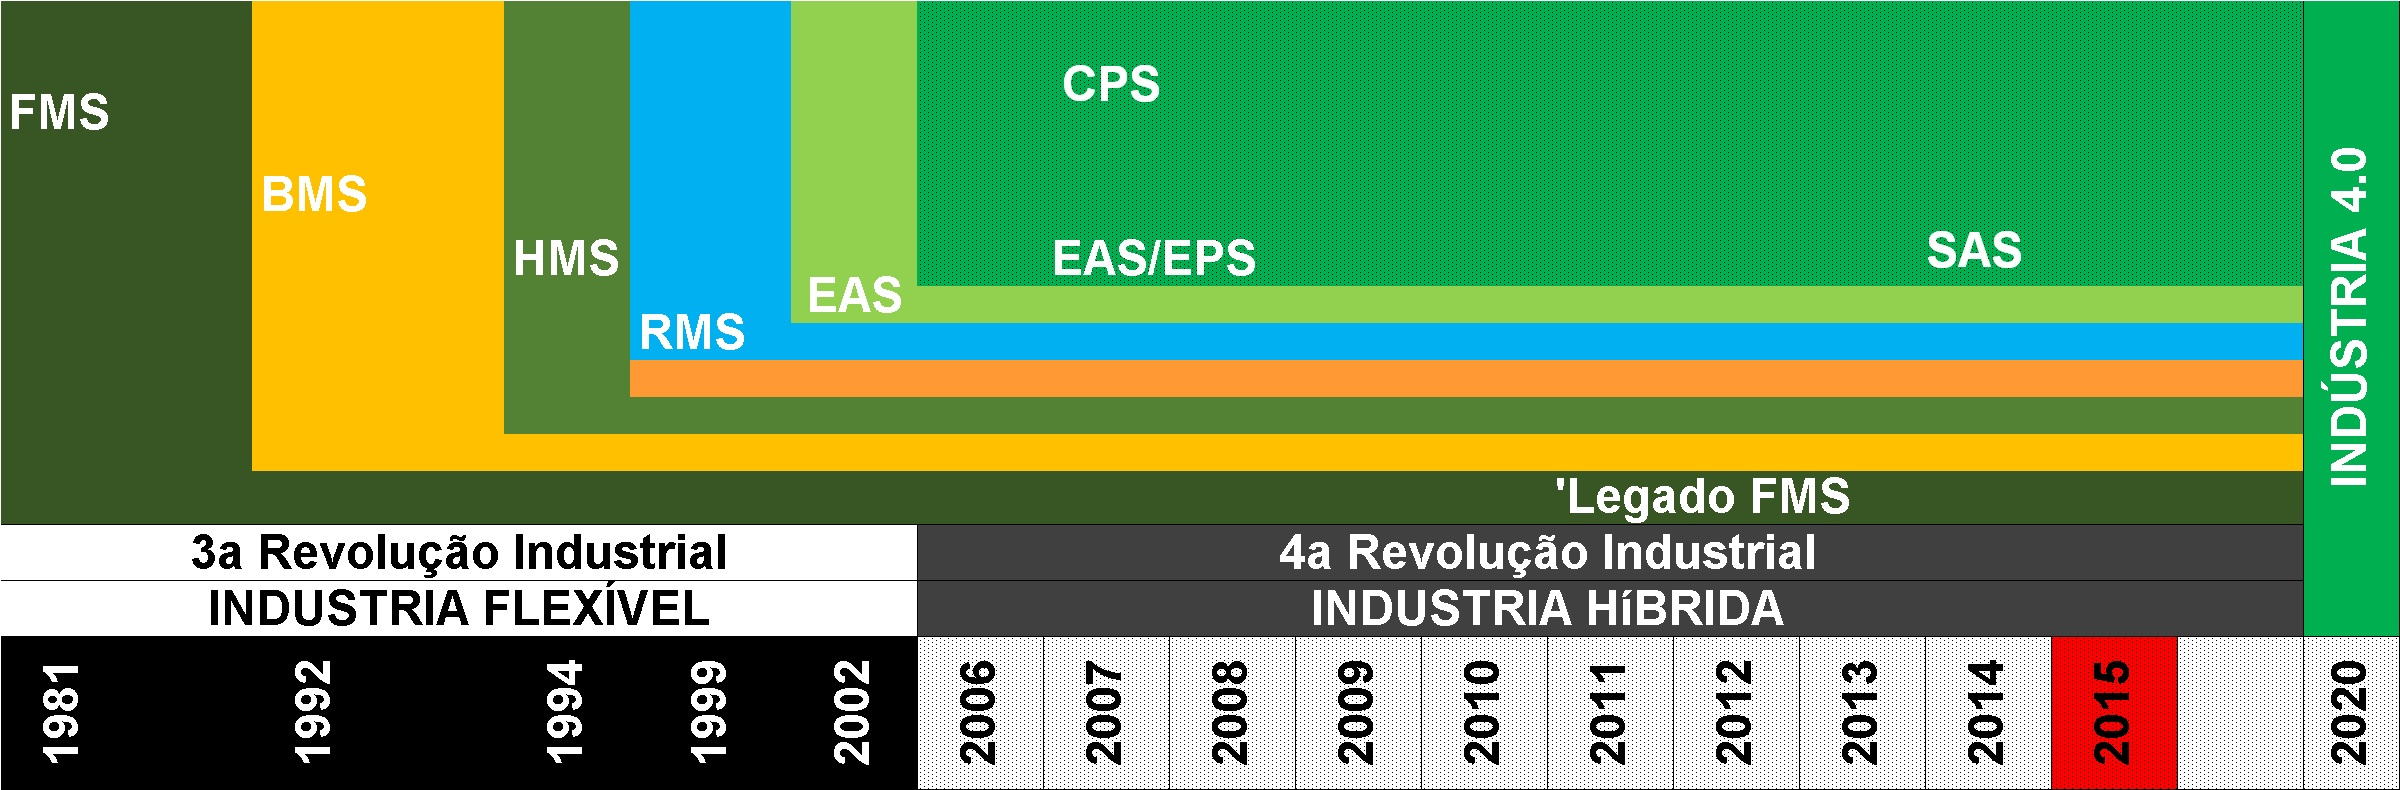
\includegraphics[width=\textwidth]{img/F0_MeDSE_PARADIGMAS_0_V2.jpg} 
	\caption{SIAPE: Paradigmas de produção}
	\label{fig:paradigmas_producao}
\end{figure*}
%================================================================
 
 
%===================================================================

\subsection{União Europeia (UE)}

%%==========================================================

\begin{figure*}[b]
	\centering
	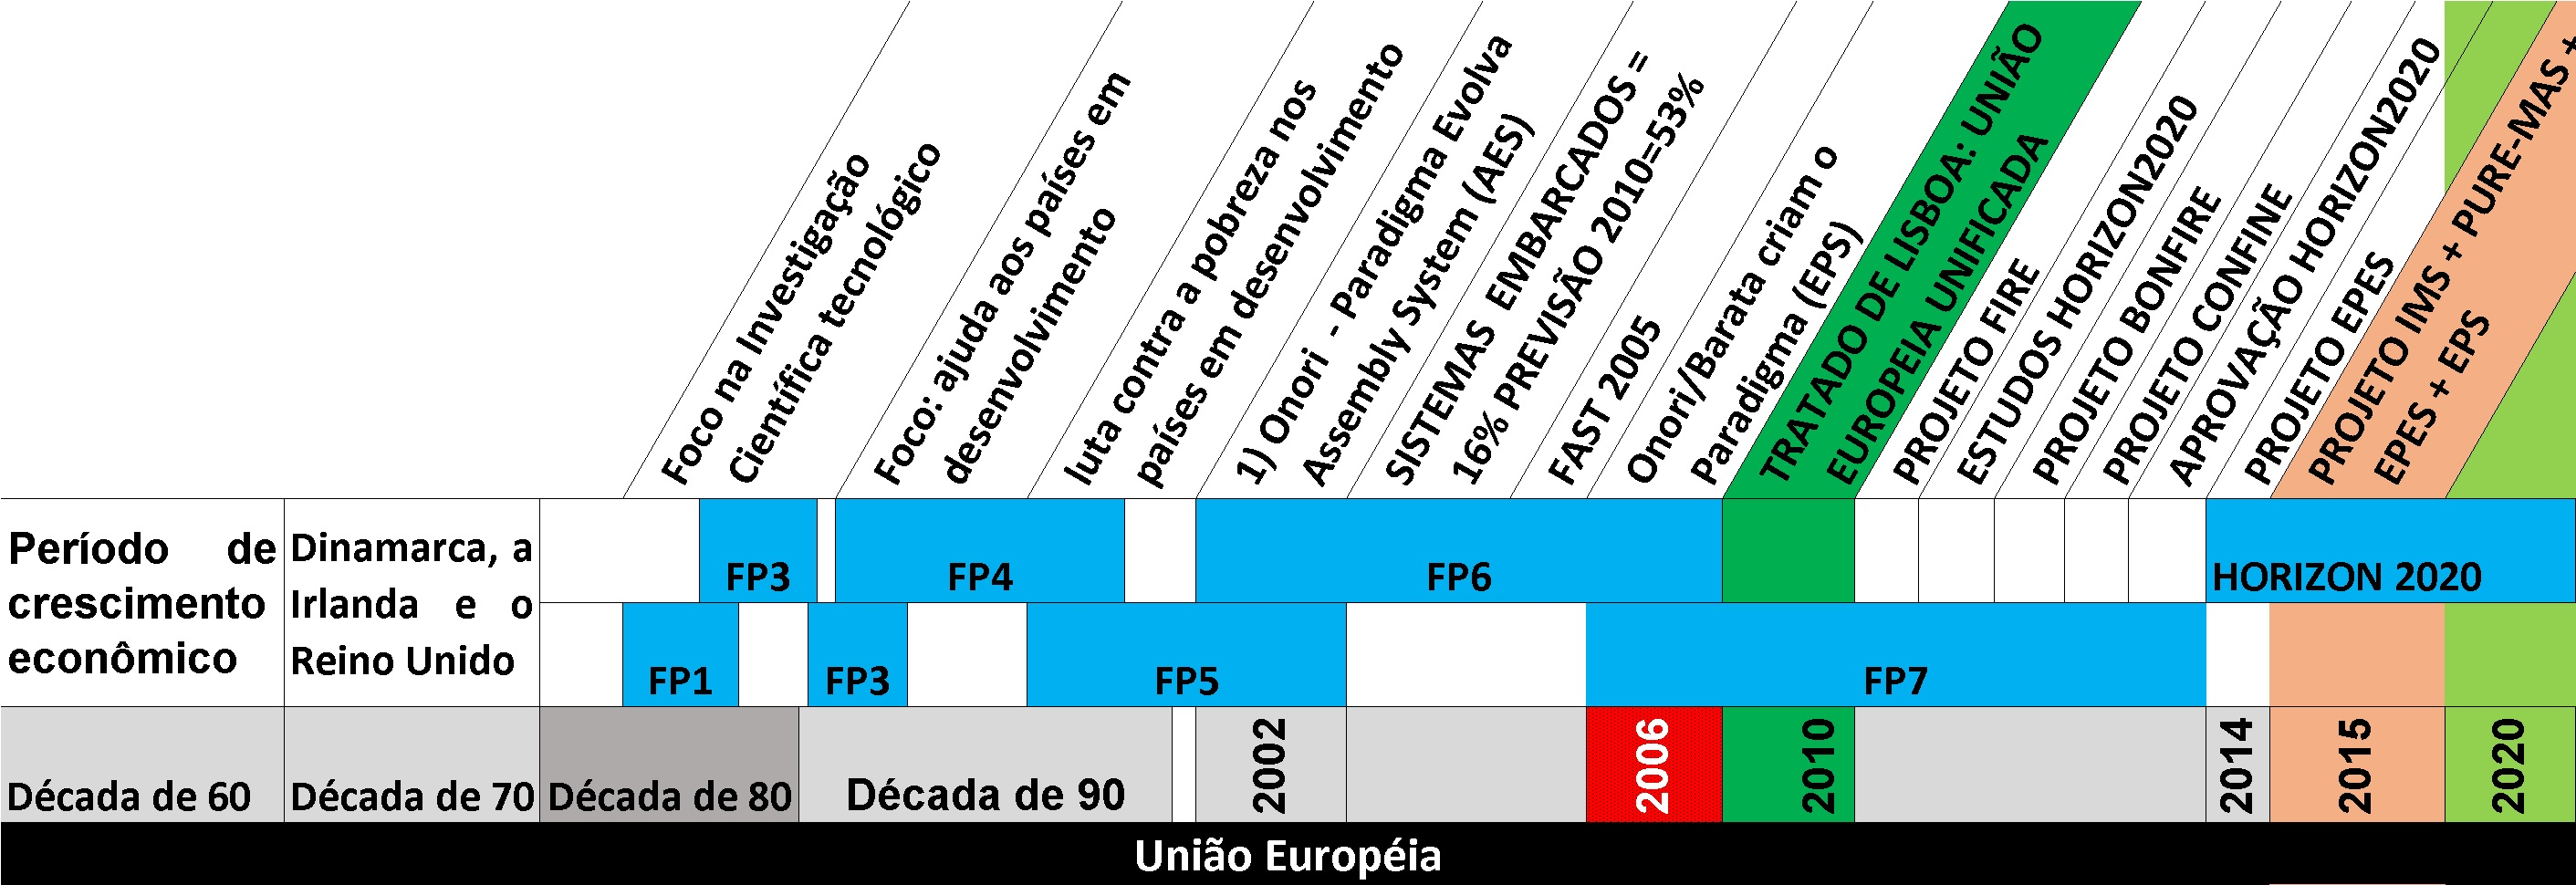
\includegraphics[width=\textwidth]{img/F1_MeDSE_UE.jpg} 
	\caption{Projetos Europeus e os sistemas evolutivos}
	\label{fig:projetos_europeus}
\end{figure*}

%%==========================================================

A Figura~\ref{fig:projetos_europeus} ilustra os principais eventos nos limites da UE e identifica os vários programas desenvolvidos desde a década de 80 até o ano 2020. Nela, igualmente, a criação do paradigma EPS em 2006 por Onori é enfatizada, assim como o Tratado de Lisboa em 2010 que concretizou a União Europeia como um bloco e possibilitou a posterior aprovação em 2013 do Programa Horizon 2020 -- com vigência de 2013 a 2020 -- que contempla os principais projetos que estão em desenvolvimento para formar os ambientes necessário para a Indústria 4.0.



%===================================================================

\subsection{Estados Unidos da América (EUA)}

A busca pela hegemonia científica e tecnológica nos EUA uniu as agências científicas, tecnológicas, militar, espacial e de segurança norte-americanas em torno das ciberestruturas~\cite{NITRDGROUPS2003}.

A Figura~\ref{F2} ilustra uma análise sobre o desenvolvimento das ciberestruturas desde a década de 60 até 2020, momento em que alguns projetos estarão sendo revisados ou concluídos. As principais iniciativas e projetos que motivaram o surgimento dos \textit{Cyber Physical System (CPS)}. O período inicia na década de 60 e se prolonga até o 2020, momento que alguns projetos estarão sendo revisado ou concluídos. Nota-se claramente que desde a década de 60 os EUA investem maciçamente nos centros de computação acadêmica, culminando na criação da ciência da computação, iniciativas em computação avançada e na criação da Internet.

Alguns marcos importantes igualmente anotados na Figura~\ref{F2}: em 2006 Hellen Gill da \textit{National Fundation Science (NFS)} cunha o termo \textit{Cyber Physical System (CPS)}~\cite{GILL2005}; em 2007 o nasce Conselho de Ciência em ciberinfraestrutura; em 2008 a comunidade acadêmica pressionou o governo~\cite{LEE2008} para uma reação conjunta; a partir de 2010 os orçamentos e projetos nos Estados unidos foram direcionados aos projetos \textit{CPS}.

\begin{figure*}[h]
	\centering
	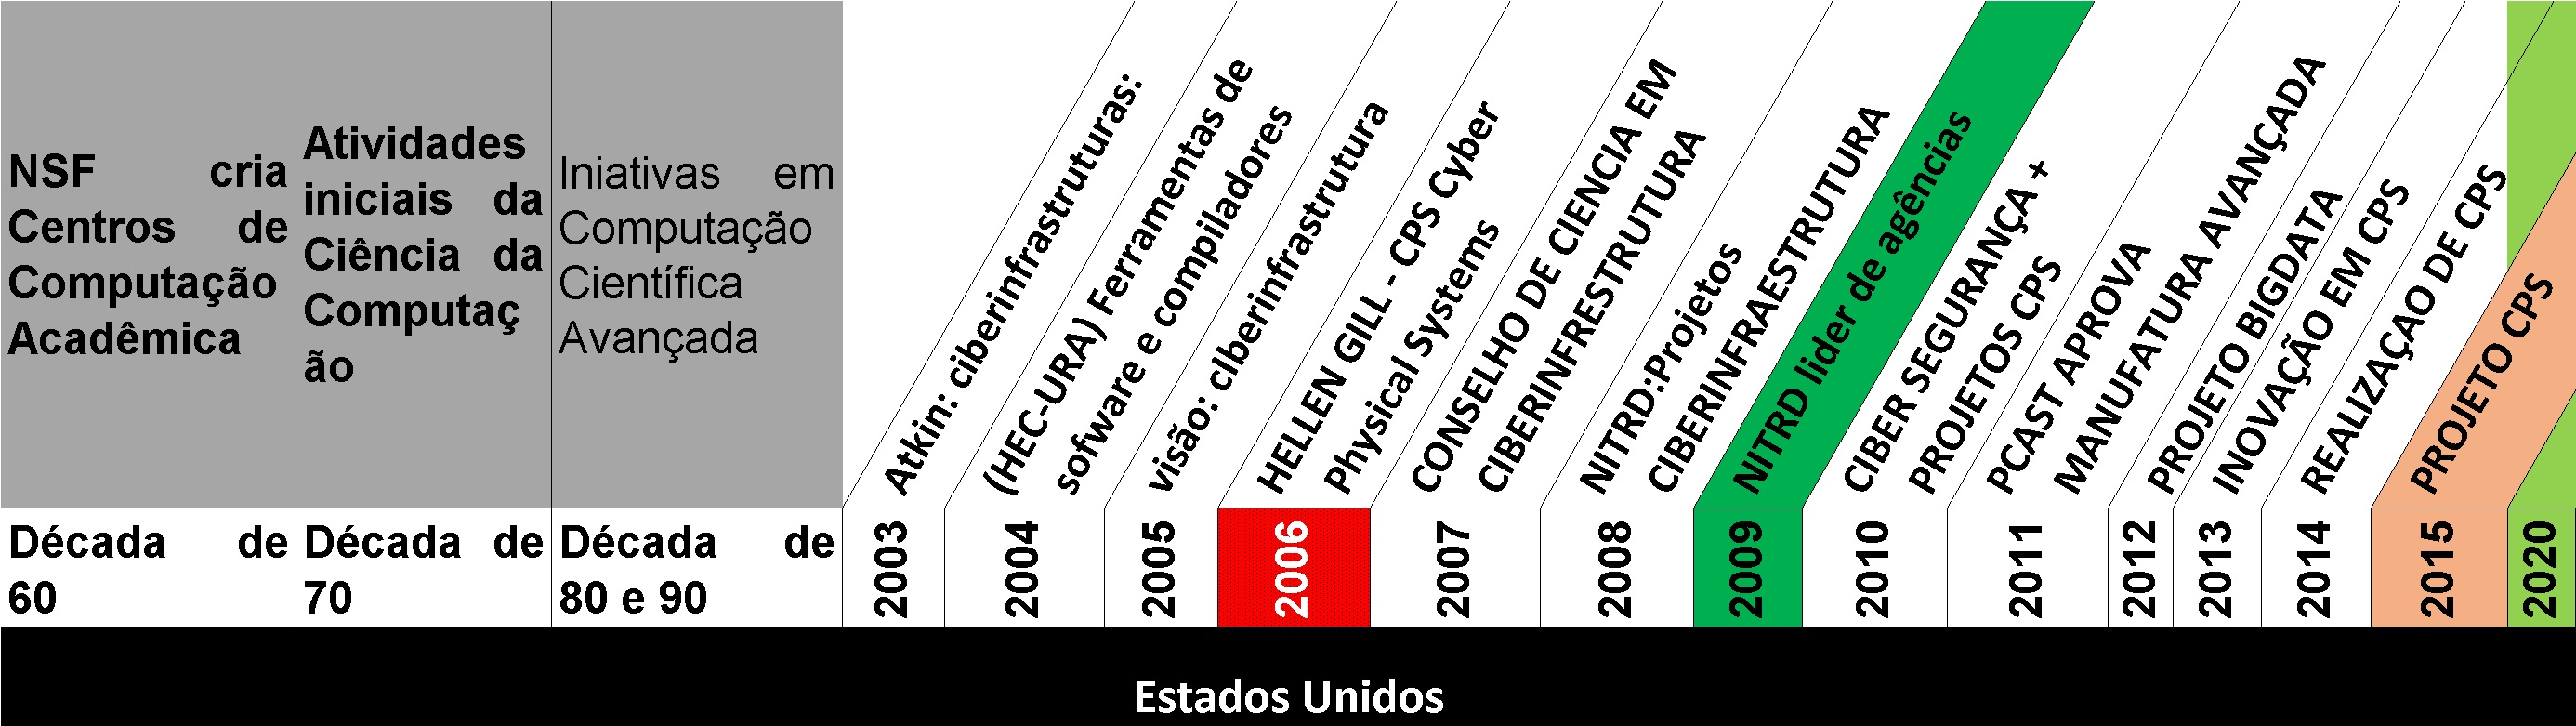
\includegraphics[width=\textwidth]{img/F2_MeDSE_USA1.jpg} 
	\caption{EUA: Linha do tempo dos CPS}
	\label{F2}
\end{figure*}


%===================================================================

\subsection{Brasil: Saindo da Indústria Mecânica e se estabelecendo na Indústria Flexível }	 


Analisando-se documentos oficiais do governo~\cite{PRESIDENCIADAREPUBLICA2014a}, os projetos, programas e estratégias em curso pelo Governo Brasileiro não evidenciam a inclusão do Brasil no círculo de países que iniciarão dentro da Plataforma da Indústria 4.0, isso dado o seu distanciamento tecnológico, a falta de sistemas baseados nos paradigmas emergentes, das fábricas inteligentes e a falta de integração entre as metas do Governo, da Indústria~\cite{CNI2013} e da Academia~\cite{CAPESVI2011}. Essa falta de integração e interação de estratégias, em moldes como acontecido na UE e EUA, condicionará o Brasil a receber o legado da Indústria Flexível e permanecer à margem da Indústria 4.0.


%===========================================================================================================

A Figura~\ref{fig:brasil_atraso} ilustra a contextualização da Indústria Brasileira que ainda está se adequando à Indústria Flexível. Nesta figura pode-se ver as chamadas revoluções industriais, que são identificadas por R1, R2, R3 e R4.  A fase entre R3 e R4 aqui é definida aqui como \emph{Indústria Híbrida}, dada a condição de sobrevivência, no mesmo espaço industrial de vários dos paradigmas de manufaturas até então conhecidos.

É importante notar que o Brasil ainda detém em grande parte de seu parque industrial sistemas legados da Indústria Mecânica e está se estabelecendo na Indústria Flexível, enquanto o mundo industrializado está totalmente incorporado aos sistemas flexíveis e experimentam a Indústria Híbrida, onde coexistem os sistemas flexíveis, ágeis, ciber e evolutivos. A marca R4 representa uma situação futura, a Indústria 4.0, onde sobreviverá a indústria inteligente, a saber àquela acoplada aos ciberespaços, contendo as ciberestruturas~\cite{Atkins2003}, os dispositivos e tecnologias que serão utilizados pelas fábricas inteligentes, que por sua vez, são baseados nos paradigmas evolutivos e nos \textit{Cyber-Physical Systems}~(CPS)~\cite{LEE2008}.

%===========================
\begin{figure*}
	\centering
	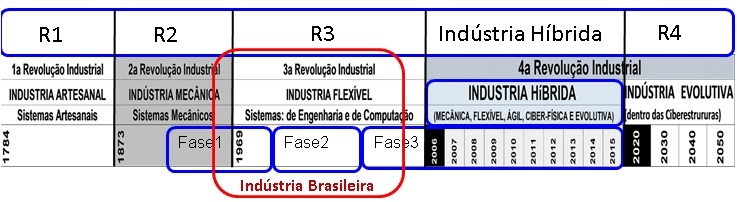
\includegraphics[width=16cm, height=5cm]{img/F3_MeDSE_GIB.jpg} 
	\caption{Brasil: Atraso da Indústria Brasileira}
	\label{fig:brasil_atraso}
\end{figure*}

%==========================================================================================================


%%========================================================================================================
\section{Tema e Problema}

Em ambientes industriais, a constante necessidade de reconfiguração das linhas de montagens é um problema recorrente. Nas atividades como a reprogramação das ferramentas de automação, braços robóticos e treinamentos de operadores de montagem, a reconfiguração é uma necessidade. Reduzir ou eliminar o tempo necessário para a reconfiguração requer mais que máquinas flexíveis, requer uma nova visão, um novo paradigma para as fábricas, bem como todo o ferramental para a aplicação deste paradigma.  		


\subsection{Delimitação do tema}
		
Considerando a contextualização global, delimitou-se o tema como \emph{Os sistemas evolutivos no contexto da Indústria 4.0 no Brasil.} 


\subsection{Especificação do problema}

Como foi colocado anteriormente, existe um problema no Brasil que é \emph{a inexistência de protótipos, no meio acadêmico e industrial, que reproduzam as propriedades dos sistemas evolutivos \textit{ (Evolvable Production System -- EPS)} a fim de permitir estudos e pequisas nas áreas de automação, controle e sistemas multi-agentes, protótipos estes capazes de ensejar a diminuição do gap tecnológico do Brasil.}

 	
\subsection{Questões de pesquisa (QP) e hipóteses relacionadas (HR)}	

	
\emph{QP1} -- Quais as características dos sistemas ágeis que podem evidenciar um sistema evolutivo de produção?
	
\emph{HR1} -- A adaptabilidade, conseguida através da reconfiguração dos parâmetros do sistema, evidenciará um sistema evolutivo de produção.

\emph{HR2} -- A evolutividade é realizada por meio da inclusão ou exclusão de módulos sem comprometer a eficiência e o funcionamento do sistema.


\subsection{Objetivo geral e específicos} 

Para realizar e comprovar essas hipóteses os seguintes objetivos foram definidos:

\begin{description}
	\item[Objetivo geral -] 
	\emph{Desenvolver um protótipo de sistema evolutivo  brasileiro baseado no paradigma \textit{EPS}}.
	
	\item[Objetivos específicos]:\par 
	
	\begin{enumerate}
	
		\item Desenvolver o módulo mecânico intercambiável, com interface elétrica;
		
		\item Desenvolver berço mecânico, com interface elétrica, para o módulo intercambiável;
		
		\item Desenvolver um protótipo que represente a indústria~3.0~\textit{(I3.0)};
		
		\item Desenvolver no PC a programação do agente de produto, consoante o paradigma EPS;
		
		\item Desenvolver no PC a programação do agente de recurso, consoante o paradigma EPS;
		
		\item Desenvolver programa de agentes que conversam entre si através do padrão FIPA;
		
		\item Desenvolver o acesso hardware programado via Raspberry Pi usando Java;
		
		\item Desenvolver interface SIAPE com o usuário para realizar o plug-and-produce; 
	 
	\end{enumerate}
	
\end{description} 


\section{Proposta do trabalho de dissertação}



\subsection{A proposta do projeto}
\label{subsec:a_proposta_projeto}

As recomendações da Indústria 4.0 \cite{VDE2014} apontam para propriedades dos Sistemas Evolutivos. Os Sistemas Evolutivos são baseados em agentes inteligentes e autônomos que, interagindo entre si, realizam a cooperação de agentes mecatrônicos para a execução de um objetivo bem definido. Os sistemas evolutivos tem duas capacidades fundamentais: a capacidade de \textit{adaptação} e a capacidade de \textit{evolução}.{\tiny }

%Por \textit{adaptação} entende-se que o sistema é capaz de propor uma configuração alternativa de si mesmo para minimizar os efeitos adversos de perturbações. Adaptação é de curto prazo e, normalmente, implica \textit{auto-reconfiguração} na forma de ajustes de parâmetros.
%
%Já o termo \textit{evolução} refere-se ao sistema que é capaz de permitir a introdução ou remoção de módulos existentes sem implicar na perda de performance e/ou quebra do seu funcionamento. A evolução se caracteriza num processo de longo prazo, podendo o sistema evoluir até o limite da tecnologia ou ao limite da planta fabril.
%
%Pode-se analisar tais capacidades através dos seguintes parâmetros: 
%
%\begin{itemize}
%	\item \textit{modularidade} que denota a noção de independência entre os módulos dos sistema; 
%	
%	\item \textit{granularidade} que evidencia o quanto de informação um agente deve possuir sobre os demais agentes, e a quantidade destes, a fim de se conseguir um objetivo definido; granularidade pode ser grossa quando, por exemplo, pouca informação e poucos agentes são necessários em uma coalizão, ou fina, quando, por exemplo, uma quantidade grande de agentes e muita informação sobre eles é necessária numa coalizão.
%	
%	\item \textit{plugabilidade} que é o conceito \textit{plug-and-produce} em tempo de produção e representa a capacidade de um módulo ser inserido ou retirado do sistema sem afetar a sua funcionalidade, ou mesmo a sua performance;
%\end{itemize}
%
%Quando se diz que um sistema é \textit{reconfigurável} isto significa que este possui a habilidade de redesenhar seu layout sem comprometer o funcionamento do sistema. Então, a plugabilidade é uma forma de reconfigurabilidade.
%	
%Quando um sistema possuir algum grau desses parâmetros, ele é dito ser \textit{auto-organizado}. Sistema auto-organizáveis são naturalmente \textit{dinâmicos}. Sistemas evolutivos possuem modularidade, plugabilidade, reconfigurabilidade e a sua granularidade pode ser ajustada conforme a complexidade do sistema.

Este trabalho visa, pois, o desenvolvimento de um sistema deste tipo, o \textbf{Sistema Inteligente Ágil de Processo Evolutivo (SIAPE)}~que é formado por uma planta composta de quatro partes que funcionam integradamente para reproduzir as duas características básicas dos sistemas EPS e pode ser analisado mediante estes quatro parâmetros.

O sistema é capaz de realizar a produção de anagramas que podem conter as seguintes letras: A, F, M, T, U. Essas letras são carimbadas em uma folha de papel contida em um carro que movimenta-se em uma esteira. Tais letras representam os processos que são realizados em sistemas industriais reais. Esses módulos são implementados como agentes inteligentes, e podem ser inseridos ou subtraídos do sistema para a concretização dos anagramas (produtos) e nas quantidades que se queira (lotes de produção), a partir de ordens de produção. Tais ordens são organizadas autonomamente em planos de produção de produtos. Quando há uma mudança na produção, isto é, a entrada de outra ordem para um novo anagrama, com quantidades diferentes, o sistema não tem a necessidade de reconfiguração entre tais produtos e lotes. E, finalmente, deve contar com o \textit{plug-and-produce}, isto é, na necessidade de uma letra desenvolvida posteriormente ao próprio sistema de montagem, este deve ser capaz de operar com a entrada de novos módulos de letras (em nosso exemplo: ``E'') como parte de seu funcionamento normal.


%==============================================================

\subsection{Metodologia da pesquisa}

A Figura \ref{fig:metodologia} ilustra a metodologia e facilita o entendimento entre os dois processos utilizados no desenvolvimento do SIAPE.

\begin{figure*}[h]
	\centering
	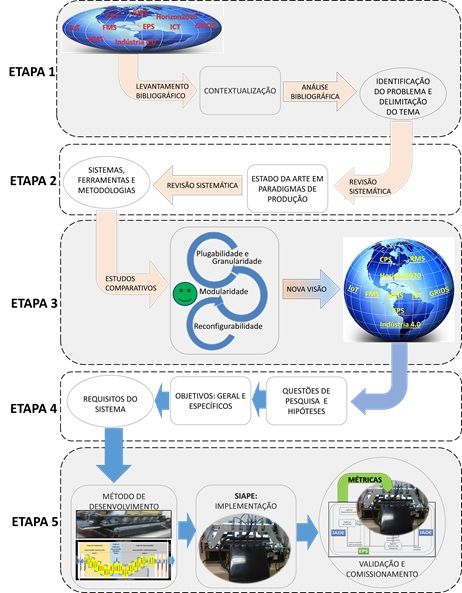
\includegraphics[height=0.8\textheight]{img/F4_SIAPE_METODOLOGIA_V0.jpg} 
	\caption{SIAPE - Metodologia da pesquisa}
	%\footnotesize{Fonte: Adaptado de~\cite{MUNZLINGER2012,MONTEBELO2000,SAMPAIO2007}}
	\label{fig:metodologia}
\end{figure*}

\begin{enumerate}
	
	\item ETAPA 1 - Objetivou o estudo do cenário atual como forma de evidenciar os principais pontos para a contextualização, e nos limites dessa, identificar um problema para ser tratado e a delimitação do tema da pesquisa.
	
	\item ETAPA 2 - Objetivou evidenciar o estado da arte considerando o tema delimitado, e baseado neste a elaboração das questões de pesquisa e hipóteses.
	
	\item ETAPA 3 - Nesta etapa foram definidas as propriedades e características que deveriam estar presentes no sistema desenvolvido.
		
	\item ETAPA 4 - Essa etapa teve como meta a elaboração dos requisitos, a partir das questões de pesquisas e das hipóteses relacionadas.
			
	\item ETAPA 5 - Nessa etapa o sistema foi implementado seguindo um método de desenvolvimento,  foram realizadas experimentações e o sistema foi validado por meio das métricas previamente definidas.
	
\end{enumerate}	
	
A Etapa 4 forneceu os requisitos do sistema com bases nas questões de pesquisa e nos objetivos geral e específicos. Esses requisitos foram tratados por um método de desenvolvimento também criado, por necessidade, para o desenvolvimento de sistemas evolutivos; o método realiza, de uma forma sistematizada, o desenvolvimento de um EPS por meio de três fases: a fase de concepção do sistema, a fase de implementação e a fase de comissionamento e finalização. Este método é explicado no Capítulo 3 e uma aplicação dele no desenvolvimento do SIAPE encontra-se detalhado no Capítulo 4.
	 

\subsection{Contribuições relevantes } 

Pode-se enumerar, dentre outras, as seguintes contribuições deste trabalho:

\begin{enumerate}
\item os dois protótipos: um flexível para reproduzir a condição atual da Indústria 3.0 (\iTresZero) e um evolutivo, que comporte as propriedades do paradigma EPS e da Plataforma da Indústria 4.0, que podem auxiliar projetistas, especialistas e acadêmicos no estudo de sistemas evolutivos;

\item uma arquitetura para os sistemas evolutivos que integre as recomendações da Indústria 4.0 (\iQuatroZero) com a performance do paradigma evolutivo de produção;

\item a metodologia para desenvolvimento de sistemas evolutivos.
\end{enumerate}
%========================================================================

\clearpage
\section{Organização do trabalho}

%\phl{Refazer, conforme o caso}

%\hl{OK. Aguardarei o término das revisões para processar este item}.

Este capítulo foi elaborado para descrever um breve resumo da contextualização global, identificar o tema e delimitar o problema a ser tratado, as questões de pesquisa utilizadas, os objetivos geral e específicos da proposta de trabalho,além das motivações e a metodologia utilizada. Os capítulos restantes desse trabalho estão dividido conforme segue. 

A Revisão da Literatura está descrita no Capítulo 2 que identifica as três revoluções industriais e alguns pontos que evidenciam a 4ª Revolução Industrial. Apresenta uma seção sobre EPS, objeto desta pesquisa. A conceituação teórica de alguns termos importantes e, finalmente, alguns trabalhos e pesquisas que se configuram como o estado da arte em sistemas evolutivos.

O Capítulo 3 descreve o desenvolvimento do SIAPE  e o método de desenvolvimento que foi criado para desenvolvê-lo.

No Capítulo 4 encontra-se a experimentação realizada por meio de um estudo de caso elaborado para evidenciar a operacionalidade do sistema.

No Capítulo 5 alguns resultados da experimentação são analisados, o sistema validado, e também são feitas alguns discussões em torno dos  resultados conseguidos na experimentação.

As conclusões encontram-se registradas no Capítulo 6, além dos trabalhos futuros que possam ser desenvolvidos a partir dos resultados desse trabalho de pesquisa.
\chapter{Conceitos}
\label{cap:conceitos}

Este capítulo está dividido em várias seções, a saber: a primeira seção identifica o panorama dos paradigmas de produção considerando os períodos conhecidos como 1ª, 2ª e 3ª revoluções industriais, bem como identifica alguns pontos que evidenciam a 4ª Revolução Industrial; a segunda seção apresenta um estudo específico sobre EPS, que é o paradigma deste trabalho; a terceira seção mostra a conceituação teórica de alguns termos importantes para o entendimento do assunto; e a última seção identifica as pesquisas e trabalhos que se configuram como o estado da arte em sistemas baseados no paradigma evolutivo.



%===================================================================

\section{Panorama dos paradigmas de produção até os dias atuais}	

\subsection{Revoluções industriais}

A Figura \ref{F9} ilustra um breve panorama do período iniciado com a primeira revolução industrial até o futuro próximo. Nela, nota-se que, após o período feudal, o nascimento da Primeira Revolução Indústria, onde a produção artesanal (realizada por máquinas artesanais) perde espaço para a produção em massa (produção de lotes grandes e realizada por máquinas mecânicas) da indústria mecânica da Segunda Revolução Industrial. Com o advento da Terceira Revolução Industrial passe a produzir lotes médios através das máquinas flexíveis. 

O problema da personalização de produtos surge também nessa época. Para tratar tal problema, surgem máquinas ágeis (baseada nos paradigmas BMS, RMS e HMS, detre outros) e esta fase é aqui identificada com indústria híbrida. Nos dias atuais surge o fenômeno da customização em massa e, para lidar com os lotes pequenos e a alta variabilidade destes, surgem os sistemas emergentes baseados nos paradigmas EAS/EPS e a auto-organização. A chamada Quarta Revolução Industrial, a caminho, é baseada principalmente nos paradigmas ágeis e evolutivos de produção. 

Nesta seção são evidenciados o surgimento dos paradigmas e comentados alguns conceitos surgidos após esse período.

%==================================================================
\begin{figure}
	\centering
	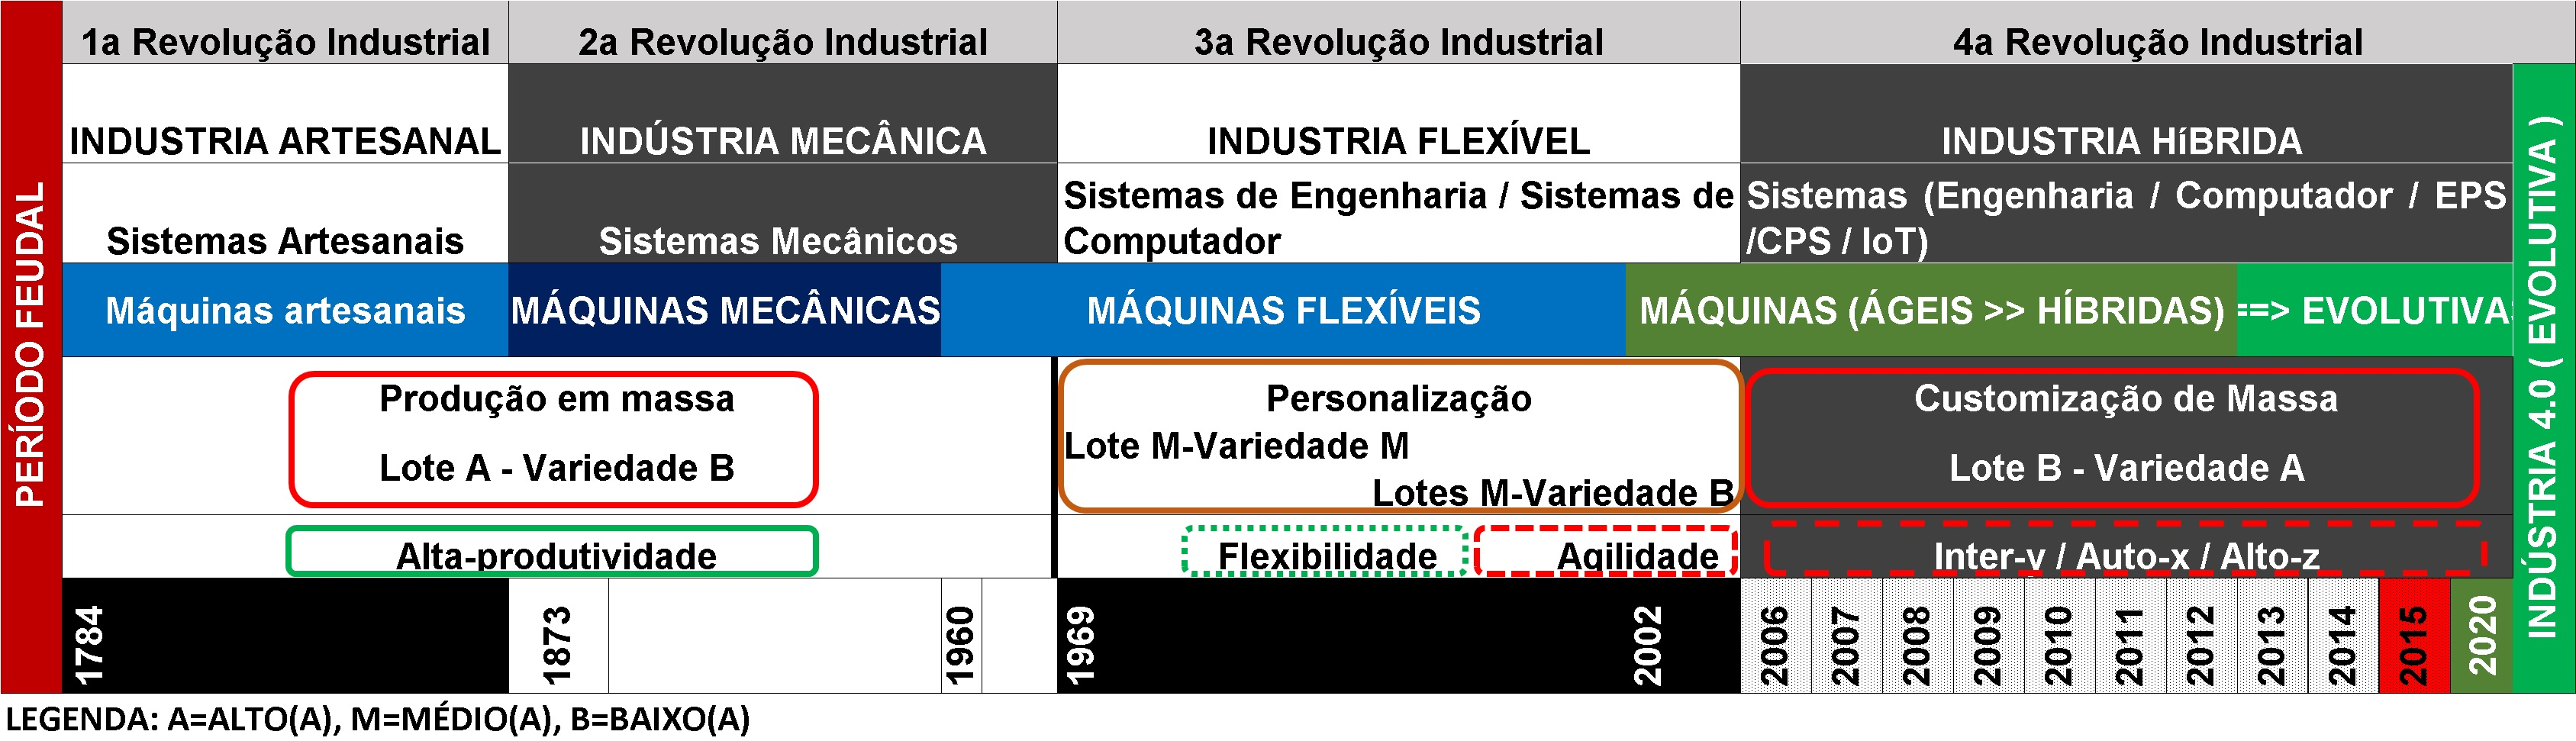
\includegraphics[width=16cm, height=6cm]{img/F9_MeDSE_RI_FULL3.jpg} 
	\caption{Revoluções Industriais, problemas e soluções}
	%{\footnotesize{Fonte: \cite{KOREN1999}}}
	\label{F9}
\end{figure}
%==================================================================

\subsection{Da máquina de Heron às máquinas flexíveis}	

Desde que os processos manuais artesanais foram substituídos por processos industriais, com o advento da Revolução Industrial, avanços tecnológicos têm causado mudanças no sistema de produção \cite{NAHER2008}. Com o advento da \textit{máquina a vapor}, um melhoramento da \textit{Máquina de Heron}, e a criação do tear mecânico, por volta de 1784, teve início o período conhecido como a $1^a$ Revolução Industrial, período no qual relevantes avanços científicos e sociais foram conseguidos naquela sociedade advinda de um sistema de feudos. Durante esse período a indústria ficou conhecida por suas características ainda artesanais como Indústria Artesanal. Esse período durou até o surgimento da eletricidade em 1873, fato que marcou o início da $2^a$ Revolução Industrial e a indústria passou de artesanal para mecânica. Nessa Indústria Mecânica, elevados lotes de produção foram conseguidos para atender às massas, que foram uma crescente demanda na Europa e nas Américas \cite{DRATH2014}

A Indústria Mecânica deu lugar à Indústria Flexível devido aos avanços tecnológicos conseguidos a partir de 1969 no campo da Eletrônica, em especial a  produção do primeiro controlador lógico programável (PLC) e significativos avanços na Tecnologia da Informação \cite{NAHER2008}.



\subsection{O surgimento dos sistemas flexíveis baseados no paradigma \textit{FMS}}	

Com a continuidade do desenvolvimento tecnológico, as máquinas flexíveis foram integradas e transformaram-se em sistemas e mostraram uma nova maneira de aumentar a produtividade, isso no ano de 1967 \cite{KOREN1999}.

Na Alemanha, em 1969, os sistemas \textit{Flexible Manufacturing System (FMS)}  foram instalados na empresa \textit{Heildlenberger Druckmaschinen} com a cooperação da Universidade de \textit{Stuttgart}. Em 1972 na exposição de \textit{Stanki} os sistemas \textit{FMS} foram demonstrados para os russos. O Japão teve seu primeiro \textit{FMS} em 1985 instalado na \textit{Fuji Xerox} \cite{GROOVER2011}. 

O trabalho desenvolvido por \citeonline{ELMARAGHY1982} deixou claro como os sistemas \textit{FMS} foram utilizados para resolver o problema da produtividade dos lotes de volume médio mas que começavam a se apresentar recheados de variedades, o que aumentava os custos e reduzia os lucros. Como o sistema produtivo \textit{FMS} podia ser, além de reprogramado, reconfigurado, este permitiu a produção de produtos sob demanda em médias quantidades, com melhores custos, e a indústria passou, então, a colocar no mercado produtos personalizados, ou seja, seguindo as preferências do cliente. Com a constante utilização de sistemas \textit{FMS}, logo se percebeu que a solução proposta para os lotes médios já não tinha a mesma eficácia. Quando essas quantidades tendiam a valores menores, a personalização de produtos passou a ser um problema. 

Neste texto, o termo \textit{personalização} é utilizado para representar um nível menor de \textit{customização}. A \textit{customização} é caracterizada por uma produção variada de produtos com curtos ciclos de vida~\cite{QUINTELA2005}.

\subsection{O surgimento dos sistemas emergentes baseados em \textit{BMS}, \textit{HMS} e \textit{RMS}}

Para enfrentar os desafios da agilidade e urgência impostos pela personalização, foi proposto por Ueda o paradigma \textit{Bionic Manufacturing System (BMS)}~\cite{UEDA1992}, que inspirou-se nos sistemas biológicos para realizar analogias com o  sistema produtivo e propor uma solução para a personalização. 

Ainda na década de 90, surge o paradigma \textit{Holonic Manufacturing System (HMS)}~\cite{CHRISTENSEN1994,VANBRUSSEL1998}  que considerou para suas análises, o sistema produtivo como um sistema composto por \textit{holons} que trocavam informações entre si. 

Ao final da década de 90, pode-se perceber um novo paradigma: \textit{Reconfigurable Manufacturing System (RMS)}~\cite{KOREN1999}, que prometia sistemas capazes de serem reconfiguráveis no chão-de-fábrica, cujos componentes eram máquinas e controladores reconfiguráveis, elaborados com metodologias para uma concepção sistemática e reposta rápida às exigências das bruscas alterações de demanda nos mercados globalizados.
 
Com o aumento da personalização possibilitado pelos sistemas \textit{FMS}, os consumidores passaram a exigir essa personalização para outros tipos de produtos, refletindo um aumento das exigências dos clientes. A tendência se concretizou e a fabricação de produtos sob medida, refletindo a preferência do cliente, passou a ser lugar comum nos mercados globalizados, e o fenômeno recebeu o nome de customização em massa \cite{DAVIS1997}, pois além de produzir o produto, o produtor deveria atender às especificações de qualidade definidas pelo usuário do produto. 

Mais recentemente, nos anos 2000 foi proposto, por Onori o paradigma \textit{Evolvable Assembly System (EAS)}~\cite{ONORI2002,FREI2006} que serviu de base para o paradigmas \textit{Evolvable Production System (EPS)}~\cite{ONORI2010}. O paradigma \textit{EPS} utiliza o conceito de agentes inteligentes para realizar as operações dentro do sistema produtivo. EPS permite a implementação de um sistema que atende a duas das características desejadas na manufatura: auto-organização e auto-otimização. Estas por sua vez permitem a produção de produtos diferentes, não necessariamente definidos com o processo produtivo, e a otimização do uso de alguns dos recursos do sistema.

%Essas soluções buscam sistemas com características de flexibilidade, agilidade, interoperabilidade, e sistemas que tenham propriedades auto-x \cite{RIBEIRO2013}, ou seja, tenham propriedade de auto-organização, auto-otimização, autoconfiguração, entre outras. 



\subsection{O surgimento da \textit{IoT}, dos \textit{CPS} e da Indústria 4.0 }	

Além das soluções propostas por pesquisadores europeus para solucionar o problema da personalização, outras iniciativas padronizadas, claras e objetivas de instituições e governos estão sendo realizadas. Por exemplo, os últimos avanços da tecnologia, conseguida pelo \textit{Massachusetts Institute of Technology (MIT)}, configuram um ambiente conhecido como \textit{Internet of Things (IoT)} \cite{STANKOVIC2014}.


A IoT é um conjunto de princípios e protocolos que visam a interligação de dispositivos ubíquos ao meio. Notadamente, quando aplicada à manufatura, está fazendo surgir a Indústria 4.0 (\iQuatroZero)~\cite{DRATH2014}. A \iQuatroZero \ é, neste momento, um cenário futurista onde as ciberestruturas existirão de fato e os dispositivos estarão preparados, testados e aprovados para funcionar dentro dessa nova realidade.

Algumas importantes conceitos da IoT são:


\begin{description}
	
\item[\textit{Plug \& Work}]-
Conceito de \textit{plug-and-produce} considerado de um ponto de vista da abordagem IoT. Sua realização no chão de fábrica implica na realização da manufatura ágil. 

\item[Manufatura Ágil] - uma abordagem de produção fortemente baseada na disponibilidade da tecnologia de fabricação de apoio que pode ser facilmente reconfigurado para responder rapidamente às mudanças do mercado, mas continua a fornecer controle total, de custos e de qualidade da produção. Manufatura ágil é universalmente considerada como o próximo passo após a metodologia de produção enxuta.

\item[Fábricas ágeis na abordagem \textit{IoT}] - as fábricas ágeis na abordagem \textit{IoT} devem ter sistemas produtivos capazes de corrigir falhas, e mudar-se devido a alterações externas relevantes, como por exemplo, a mudança no tipo de produtos para os quais devem ser produzidos ou no volume de produção. Agilidade pode, pois ser necessária em muitos níveis diferentes, por exemplo, adaptação recursos para falhas de rede ou aumento de carga, ao nível do processo, onde as novas necessidades são imediatamente adaptadas.

\end{description}


%===================================================================

\section{Sistemas Evolutivos de Produção - \textit{EPS}}

Os sistemas evolutivos são baseados em agentes inteligentes e autônomos que são capazes de cooperarem entre si. Esta cooperação leva tais sistemas a possuírem a capacidade de \textit{adaptação} e de \textit{evolução}~\cite{ONORI2002}.

Conforme mostrado na Seção~\ref{subsec:a_proposta_projeto}, por \textit{adaptação} entende-se que o sistema é capaz de propor uma configuração alternativa de si mesmo para minimizar os efeitos adversos de perturbações. Adaptação é de curto prazo e, normalmente, implica \textit{auto-reconfiguração} na forma de ajustes de parâmetros. Já o termo \textit{evolução} refere-se ao sistema que é capaz de permitir a introdução ou remoção de módulos existentes sem implicar na perda de performance e/ou quebra do seu funcionamento. A evolução se caracteriza num processo de longo prazo, podendo o sistema evoluir até o limite da tecnologia ou ao da planta fabril.

Como um sistema evolutivo é baseado em agentes autônomos que reconhecem o ambiente físico e são capazes de executar alguma ação sobre este ambiente, EPS apresenta auto-organização, isto é, o sistema é capaz de reconhecer os agentes que estiverem ativos em determinado momento e formar a sociedade de agentes necessária. Então EPS possui algum grau do \textit{plug-and-produce}, isto é, o plugar e produzir, onde cada módulo do sistema pode ser retirado ou colocado no sistema (\textit{on-line}) como parte integrante de seu funcionamento normal.

Uma característica primordial de sistemas baseados no paradigma EPS é que o foco da inteligência do processo produtivo, isto é, o conhecimento de como se faz um determinado produto, é retirada dos módulos que realizam a atividade de montagem do produto e é colocada em um agente inteligente externo àqueles módulos. 

Assim, os recursos de produção passam a ter somente a inteligência de seu próprio funcionamento. Como são autônomos, eles são verdadeiros agentes inteligentes, mas como possuem a capacidade de ação no mundo físico, através de seus sensores e atuadores, capacidade de computação própria e capacidade de comunicação com as outras entidades do sistema, são equipamentos mecatrônicos. Tais módulos são as próprias ferramenta de montagem com inteligência, mas não possuem a informação de como um produto específico é montado. Tais módulos são chamados de agentes mecatrônicos.

Sem a inteligência do processo, os recursos de produção não teriam muita utilidade em um processo produtivo, necessitando-se então que tais recursos sejam coordenados para a execução dos objetivos finais. Usando termos derivados da área de agentes, tais recursos são agentes mecatrônicos e a inteligência do processo reside em um agente de \textit{coalizão} que serve para coordenar e unir em uma sociedade de agentes, aqueles agentes mecatrônicos necessários para se produzir um determinado produto \cite{Barata2006}.

EPS segue a metáfora do LEGO\textcopyright, isto é, onde peças pequenas são unidas de uma forma inteligente para se montar elementos bem complexos. Da mesma forma, para se construir um produto usando um EPS, é necessário que o produto seja quebrado em partes suficientemente pequenas, partes essas capazes de ser montadas usando um ou mais recursos do sistema produtivo. Entretanto, também é necessário que tais recursos sejam especificados para realizar as atividades de montagem. Essas atividades são implementadas por agentes mecatrônicos, os quais expõe funcionalidades específicas para o sistema, chamadas de \textit{skills}, justamente por retratar as habilidades que aquele módulo ou agente mecatrônico possui. Se forem suficientemente básicas e gerais essas atividades, um sistema de montagem evolutivo deve ser capaz de montar uma ampla gama de produtos, i.e, o sistema passa a ter a possibilidade de montar uma alta variabilidade de produtos.

Portanto, o paradigma EPS muda o foco da inteligência, no chão de fábrica, dos equipamentos que formam o sistema produtivo para o produto. Por causa da sua arquitetura baseada em agentes inteligentes, que possuem a capacidade de auto-organização, possuem também a propriedade do ``plugar e produzir''. 

\begin{figure}[h]
	\centering
	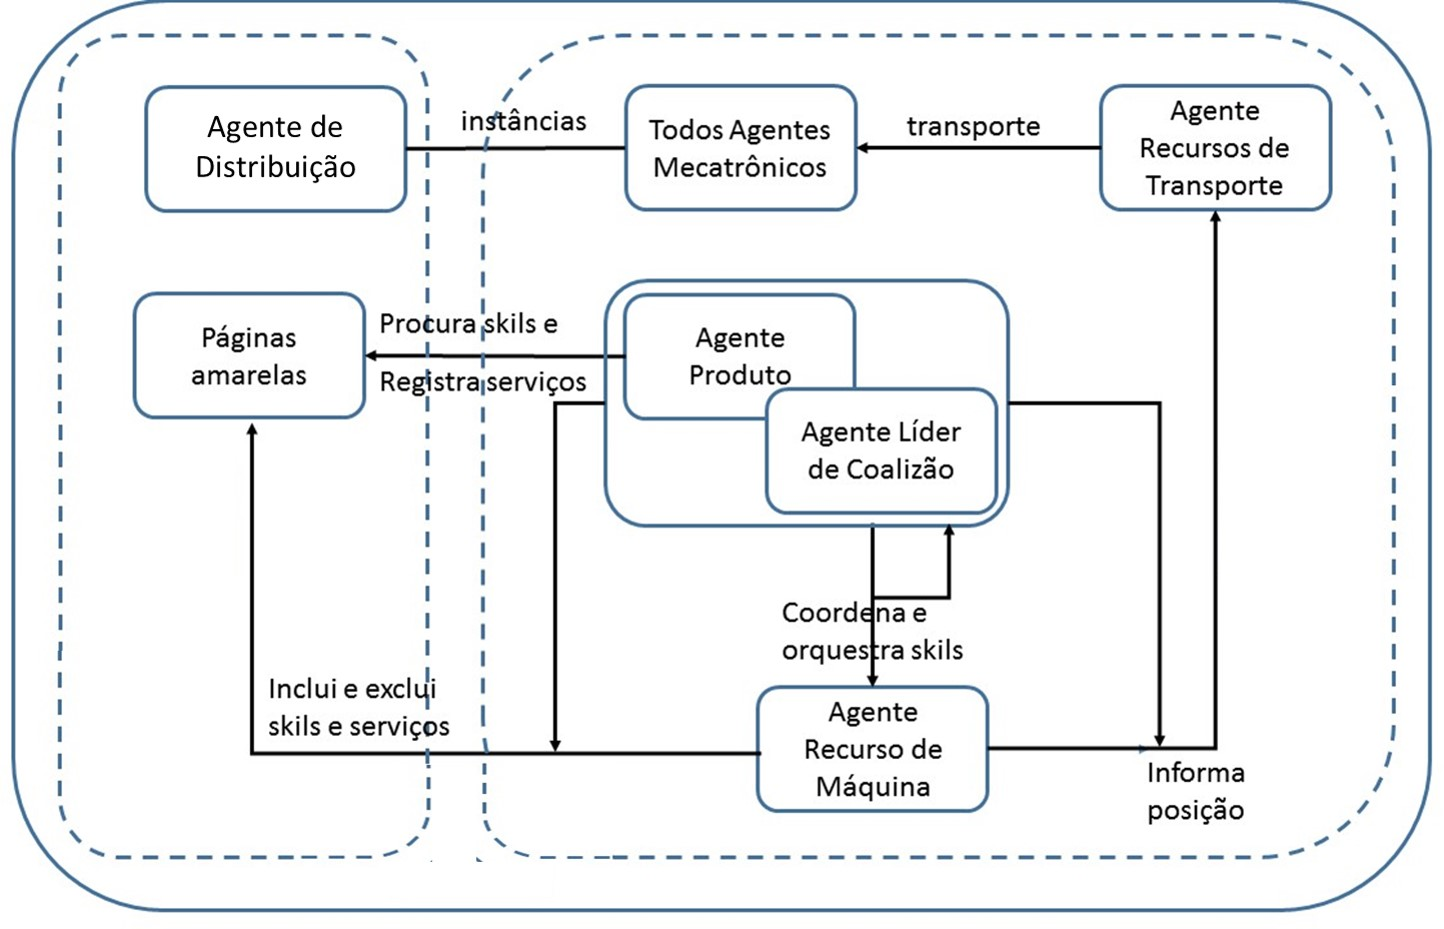
\includegraphics[width=0.8\textwidth]{img/F8_1_SIAPE_Arquitetura_EPS.jpg}
	\caption{IADE: Arquitetura de referência EPS}
	\label{fig:arq_referencia_eps}
	{\footnotesize{Fonte: \cite{CAVALCANTE2012a}}}
\end{figure}

Sua arquitetura de referência pode ser vista na Figura~\ref{fig:arq_referencia_eps}, que mostra dois tipos de agentes mecatrônicos: agente de recurso e agente de coalizão. Agentes de produtos são um tipo de agente de coalizão. Agentes de transporte são um tipo de agente mecatrônico normal, mas especializado no sistema de transporte.

Tais sistemas estão sendo desenvolvidos e testados objetivando as fábricas inteligentes e a padronização proposta pela Plataforma~\cite{VDE2014} da Indústria 4.0 ~\cite{DRATH2014}. 

Historicamente, EPS é a abordagem mais nova de um movimento que começa a partir da década de 80. A Figura~\ref{fig:evolucao_paradigmas} ilustra a evolução dos paradigmas de produção, mostrando também os nomes dos pesquisadores que iniciaram aquele paradigma.

\begin{figure}[b]
	\centering
	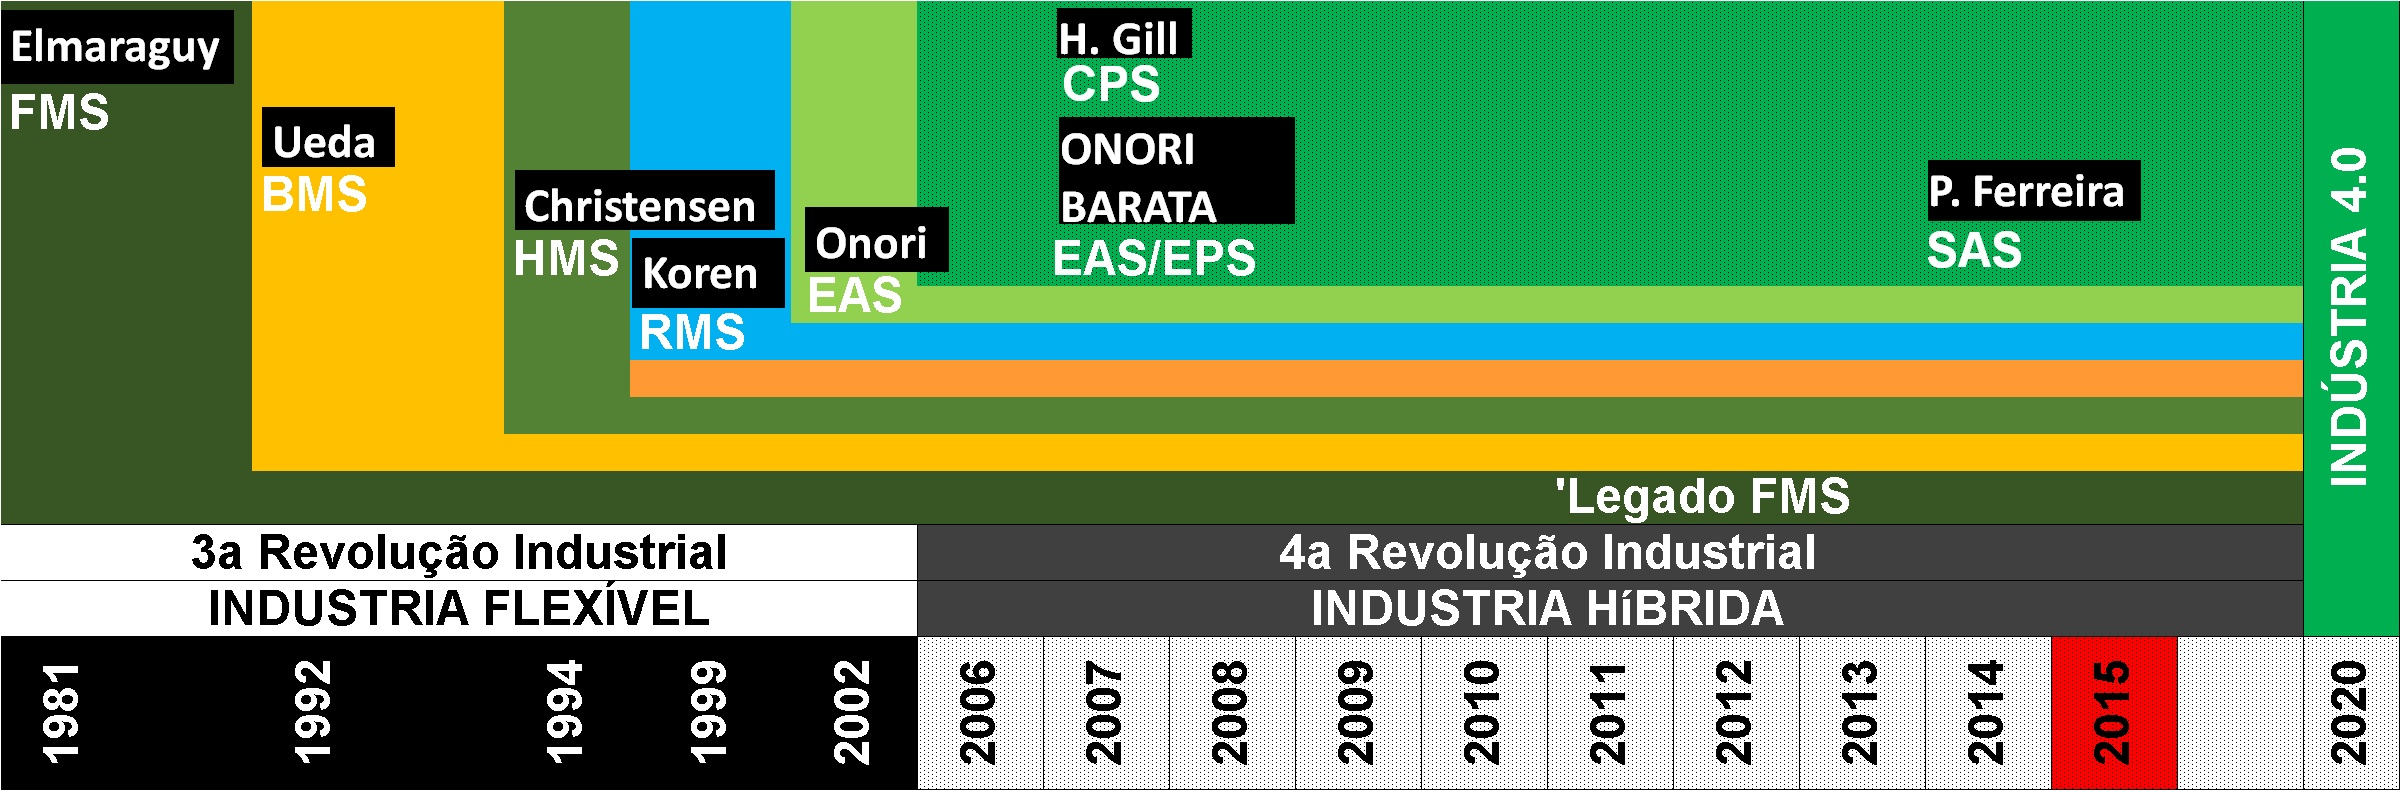
\includegraphics[width=\textwidth]{img/F8_2_SIAPE_PARADIGMAS.jpg}
	\caption{Evolução do Paradigmas de Produção}
	%\footnotesize{Fonte: O autor}
	\label{fig:evolucao_paradigmas}
\end{figure}

Os EPS possuem algumas características interessantes, pois possuem em um grau elevado, adaptabilidade, evolutibilidade, modularidade e sua granularidade pode ser ajustada conforme a complexidade do sistema. Para este trabalho, estes termos tem os seguintes significados:

\textbf{Adaptabilidade} -- o sistema tem de ser capaz de propor uma configuração alternativa para minimizar os efeitos adversos de perturbações. Adaptação é de curto prazo e, normalmente, implica \textit{auto-reconfiguração} na forma de ajustes de parâmetros~\cite{ROSA2013c}.

\textbf{Evolutibilidade} -- 
Em relação à \textit{evolução}, o sistema tem de ser capaz de permitir a introdução ou remoção de módulos existentes sem implicar na performance e no funcionamento do sistema. Assim, o sistema evolui a medida que novos produtos são colocados em produção, isto é, conforme o ambiente industrial modifica-se no tempo. A evolução se caracteriza num processo de longo prazo, podendo o sistema evoluir até o limite da tecnologia ou ao limite da planta fabril~\cite{ROSA2013c}.

\textbf{Modularidade} -- denotada pela noção de independência entre os módulos dos sistema.

\textbf{Plugabilidade} -- se o sistema pode inserir ou remover módulos como parte de seu funcionamento normal em tempo de produção.

\textbf{Granularidade} -- que evidencia o quanto de informação um agente deve possuir sobre os demais agentes, e a quantidade destes, a fim de se conseguir um objetivo definido.

Para este texto, \textbf{reconfigurabilidade} é a habilidade do sistema de redesenhar seu layout sem comprometer o funcionamento do sistema. Portanto, a plugabilidade é uma espécie de reconfigurabilidade. 

Quando um sistema possuir algum grau desses parâmetros, ele é dito possuir a \textbf{auto-organização} e o sistema é dito ser \textbf{dinâmico}.


\subsection{Visão geral da arquitetura EPS}

EPS é baseado em agentes inteligentes. Nas primeiras arquiteturas havia a definição de muitos tipos diferentes de agentes, capazes de tratar certos aspectos do sistema produtivo, tais como transporte, acesso hardware ou agentes de coalizão.

Simplificações tem sido propostas ao longo do tempo. Atualmente, EPS pode ser descrito como uma abordagem multiagente capaz de auto-organização e execução de processos complexos através da interação entre os agentes que formam o sistema. Há basicamente dois tipos de agentes em EPS: os agentes mecatrônicos e os agentes não mecatrônicos. Dentre os agentes mecatrônicos, pode-se citar a existência de dois subtipos: agentes cognitivos e agentes motores. 

Os agentes cognitivos são os responsáveis pela coalizão de outros agentes mecatrônicos: cognitivos ou motores. Os agentes motores são os que possuem acesso ao hardware elétrico e/ou mecânico do equipamento mecatrônico.

Os diversos tipos de funções no sistema produtivo são implementados por meio destes tipos de agentes. Por exemplo, um agente produto é um tipo especial de agente cognitivo que possui a inteligência de como montar a si mesmo através da coalizão dos agentes mecatrônicos (recursos/ferramentas) do sistema produtivo.

Agentes mecatrônicos possuem \textit{habilidades}, isto é, o que eles são capazes de fazer no sistema produtivo. Pode ser algo como \texttt{produzirProdutoA()} ou \texttt{baixarSugador()} ou ainda como \texttt{fecharGarra()}. \par 
Essas habilidade ou serviços que os agentes executam são chamados de \textit{skills}. \par 
Um agente mecatrônico pode possuir um ou mais \textit{skills}, que podem/são disponibilizados para todos os outros agentes do sistema.

Dentre os agentes não mecatrônicos cita-se: o agente intermediador (\textit{gateway}) que tem a função de interligar o sistema de produção EPS com outros sistemas legados e/ou interface homem máquina; e o agente de páginas amarelas (\textit{Yellow Page Agent} - YPA) que é o responsável pelo registro e busca de \textit{skills} por todo o sistema.

%=====================descrição da arquitetura EPS de Cavalcante=======================================================

\subsection{Descrição da Arquitetura EPS de Cavalcante }
 	 	  
A arquitetura \textit{EPS} proposta por Cavalcante denominada de Arquitetura Baseada em Agentes e Auto-Organizável Para a Manufatura  está ilustrada na Figura \ref{F132} e é descrita a seguir.

A arquitetura é formada por dois tipos de agentes:
 	 
 \textbf{O agente cognitivo} é o responsável pela lógica da aplicação empregada na situação e escolhe uma decisão a ser realizada, por outro agente cognitivo ou por um agente motor. A camada superior funciona como aplicação do agente e  a camada inferior funciona como interface de comunicação com os outros agentes do sistema, e promove a seleção e as requisições feitas para os outros agentes do sistema.
 	 	  
  \textbf{O agente motor} por sua vez, tem sua camada superior funcionando como comunicação e a camada inferior como a aplicação do agente. A camada superior recebe a comunicação das operações a serem realizadas que são enviadas pelo agente cognitivo. A camada inferior além de ter a função da aplicação do agente, funciona como camada de sensoriamento percebendo o ambiente e informando as condições sentidas ao agente cognitivo, para que este tome as decisões necessárias e as realize as tarefas atribuídas ao sistema.
 	 	  
  	 	  \begin{figure}
  	 	  	\centering
  	 	  	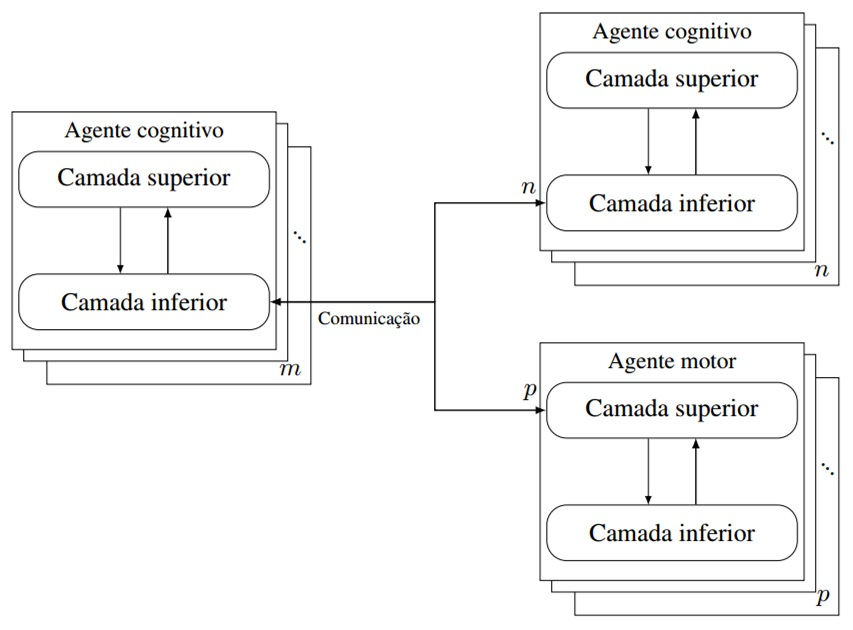
\includegraphics[width=12cm, height=7cm]{F132_ARQUITETURA_BAAOPM.jpg} 
  	 	  	\caption{Visão geral da Arquitetura proposta por Cavalcante}
  	 	  	\footnotesize{Fonte: \cite{CAVALCANTE2012a}}
  	 	  	\label{F132}
  	 	  \end{figure}
  	 	  
 	 	  \begin{figure}[b]
 	 	  	\centering
 	 	  	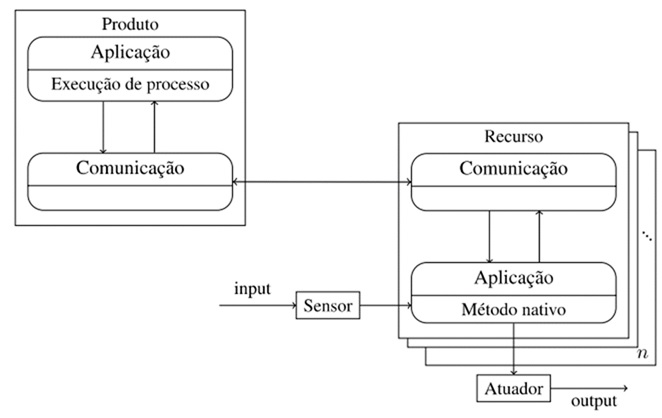
\includegraphics[width=12cm, height=6cm]{F133_ARQUITETURA_BAAOPM_MONTAGEM.jpg} 
 	 	  	\caption{Arquitetura para uma aplicação em um sistema de montagem}
 	 	  	\footnotesize{Fonte: \cite{CAVALCANTE2012a}}
 	 	  	\label{F133}
 	 	  \end{figure}	
 	 	  
 A arquitetura foi dividida para uso em dois tipos de aplicações: em sistemas de montagem e em sistemas de controle. A aplicação para um sistema de montagem é formado por agentes cognitivos, que modelam os produtos a serem montados, e por agentes motores, que modelam os recursos de hardware que realizam operações no processo de montagem. A Figura \ref{F133} ilustra a aplicação desta arquitetura para sistemas de produção. Nesta pode-se identificar o agente produto que é modelado por agentes cognitivos, e agentes motores que modelam os recursos de produção. 
 	 	  
 	 	  
 Já a Figura \ref{F138} ilustra a implementação de referência de EPS conforme o projeto \textit{IDEAS}. Os agentes desta implementação são assim chamados:
 	 	  
 	 	  \begin{description}	
 	 	  	
 	 	  	\item[\textit{DeploymentAgent (DA)}]  representa o agente de distribuição, isto é, o agente que  pesquisa serviços de páginas amarelas, os \textit{skills} que devem ser trocados entre agentes para negociação até que se atinja os objetivos propostos pelo sistema. O \textit{DA} também permite que o sistema seja configurado através de ferramentas externas.
 	 	  	
 	 	  	\item[\textit{YellowPageAgent (YPA)}] Agente Páginas Amarelas - é o responsável por registrar as habilidades dos agentes que não são mecatrônicos. Ele fornece uma infra-estrutura que permite que outros agentes registrem suas informações e que estas sejam consultadas por outros agentes que estejam necessitando de determinado \textit{skil}.
 	 	  	
 	 	  	\item[\textit{Resource Agente (RA)}] são os agentes que externam funcionalidades ao sistema de montagem. Este é o agente básico da biblioteca \textit{IADE} que controla os módulos de hardware que podem ser conectados ou desconectado no hardware do sistema, isto é, este agente é dotado de skills atômicos que são diretamente relacionado com o hardware. Este fato proporciona  ao sistema a capacidade de reconfiguração de funcionalidades no nível do controlador. 
 	 	  	
 	 	  	\item[\textit{Coalition Leader Agent (CLA)}]  são agregadores e a base da reutilização de funcionalidades em qualquer nível. É o agente que suporta a composição de competências. Isto significa que o \textit{CLA} é capaz de reagir às perturbações no ambiente, tais como a adição ou remoção de funcionalidades e falhas sob o seu domínio. 
 	 	  	
 	 	  	\item[\textit{Transport Agent (TA)}] são abstrações do sistema de transporte, isto é, é o agente que abstrai as entidades de transporte por exemplo, transportadores ou \textit{AGV}. É responsável pela computação do custo de transporte entre localizações no sistema.
 	 	  	
 	 	  \end{description}	
 	 	  
 	 	  Considerando a nomenclatura de Cavalcante, os \textit{CLAs e PAs} são agentes cognitivos e \textit{RAs e TSAs} são agentes motores.
 	 	  
 	 	  \begin{figure}
 	 	  	\centering
 	 	  	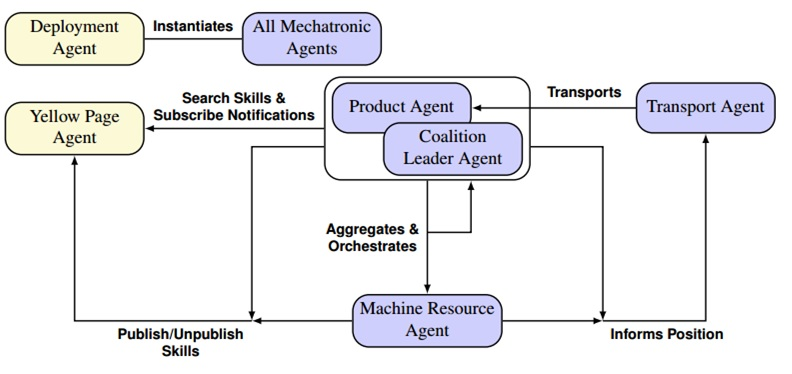
\includegraphics[width=12cm, height=6cm]{F138_IADE_cavalcante.jpg} 
 	 	  	\caption{Implementação de referência EPS}
 	 	  	\footnotesize{Fonte: \cite{CAVALCANTE2012a}}
 	 	  	\label{F138}
 	 	  \end{figure}	 


%===============================================================================================================
  \subsection{A Arquitetura do SIAPE}

%=================================================================================================================

A Figura \ref{fig:eps_arquitetura_1} ilustra a arquitetura do SIAPE que foi baseada na arquitetura de Cavalcante para um sistema de montagem. Na figura os recursos são agentes cognitivos ou agentes motores que realizam as operações do processo de montagem diretamente nos sensores e atuadores do sistema. O agente motor principal, no SIAPE, recebe o nome de AcHw. Assim como todos os módulos e agentes do SIAPE, o AcHw foi concebido a partir da aplicação do Método de Desenvolvimento de Sistemas Evolutivos (MeDSE), aplicado ao desenvolvimento do SIAPE. O método de desenvolvimento é detalhado no Capítulo 3.

O agente AcHw do SIAPE  tem a principal função de identificar, em tempo real, os módulos que estão presentes no  sistema e informá-los ao agente  \textit{YPA}. Uma vez identificados no \textit{YPA}, os demais agentes tem acesso aos \textit{skills} do AcHW, notadamente o agente Anagram, que usa essas informações para realizar o processo produtivo. 

O agente \textit{OrderAgent} instancia agentes Anagram (agente Produto na arquitetura) que conhece todas as etapas de produção que envolve o agente Stamper e o agente Conveyor. 

O operador pode se comunicar com o sistema por meio da Interface Homem Máquina (IHM) que acessa diretamente o \textit{OrderAgent}. Este também pode ser usado com a função de \textit{gateway} na comunicação tanto de sistema \iQuatroZero, isto é, sistemas aderentes à plataforma \iQuatroZero, quanto de ambientes \iTresZero, isto é, sistema flexíveis comuns aos sistemas da 3ª Revolução Industrial.

Resumindo, na aplicação de tal arquitetura neste trabalho, tem-se os seguintes agentes:

\begin{itemize}
	\item YPA - registro e busca de \textit{skills}
	
	\item OrderAgent - um \textit{gateway} para a interface homem máquina do EPS; instancia os anagramas de acordo com a ordem de serviço gerada na IHM.
	
	\item Anagram - um agente cognitivo que representa um produto a ser produzido.
	
	\item AcHw - um agente motor responsável pelo acesso ao hardware eletrônico do sistema.
	
	\item Conveyor - um agente cognitivo que representa a esteira do sistema; esconde do agente produto a complexidade do acesso ao hardware para se realizar o transporte.
	
	\item Stamper - um agente cognitivo que representa um módulo carimbador do sistema; esconde do agente produto a complexidade do acesso ao hardware para se carimbar letras do anagrama na palete.
\end{itemize}


\begin{figure}
	\centering
	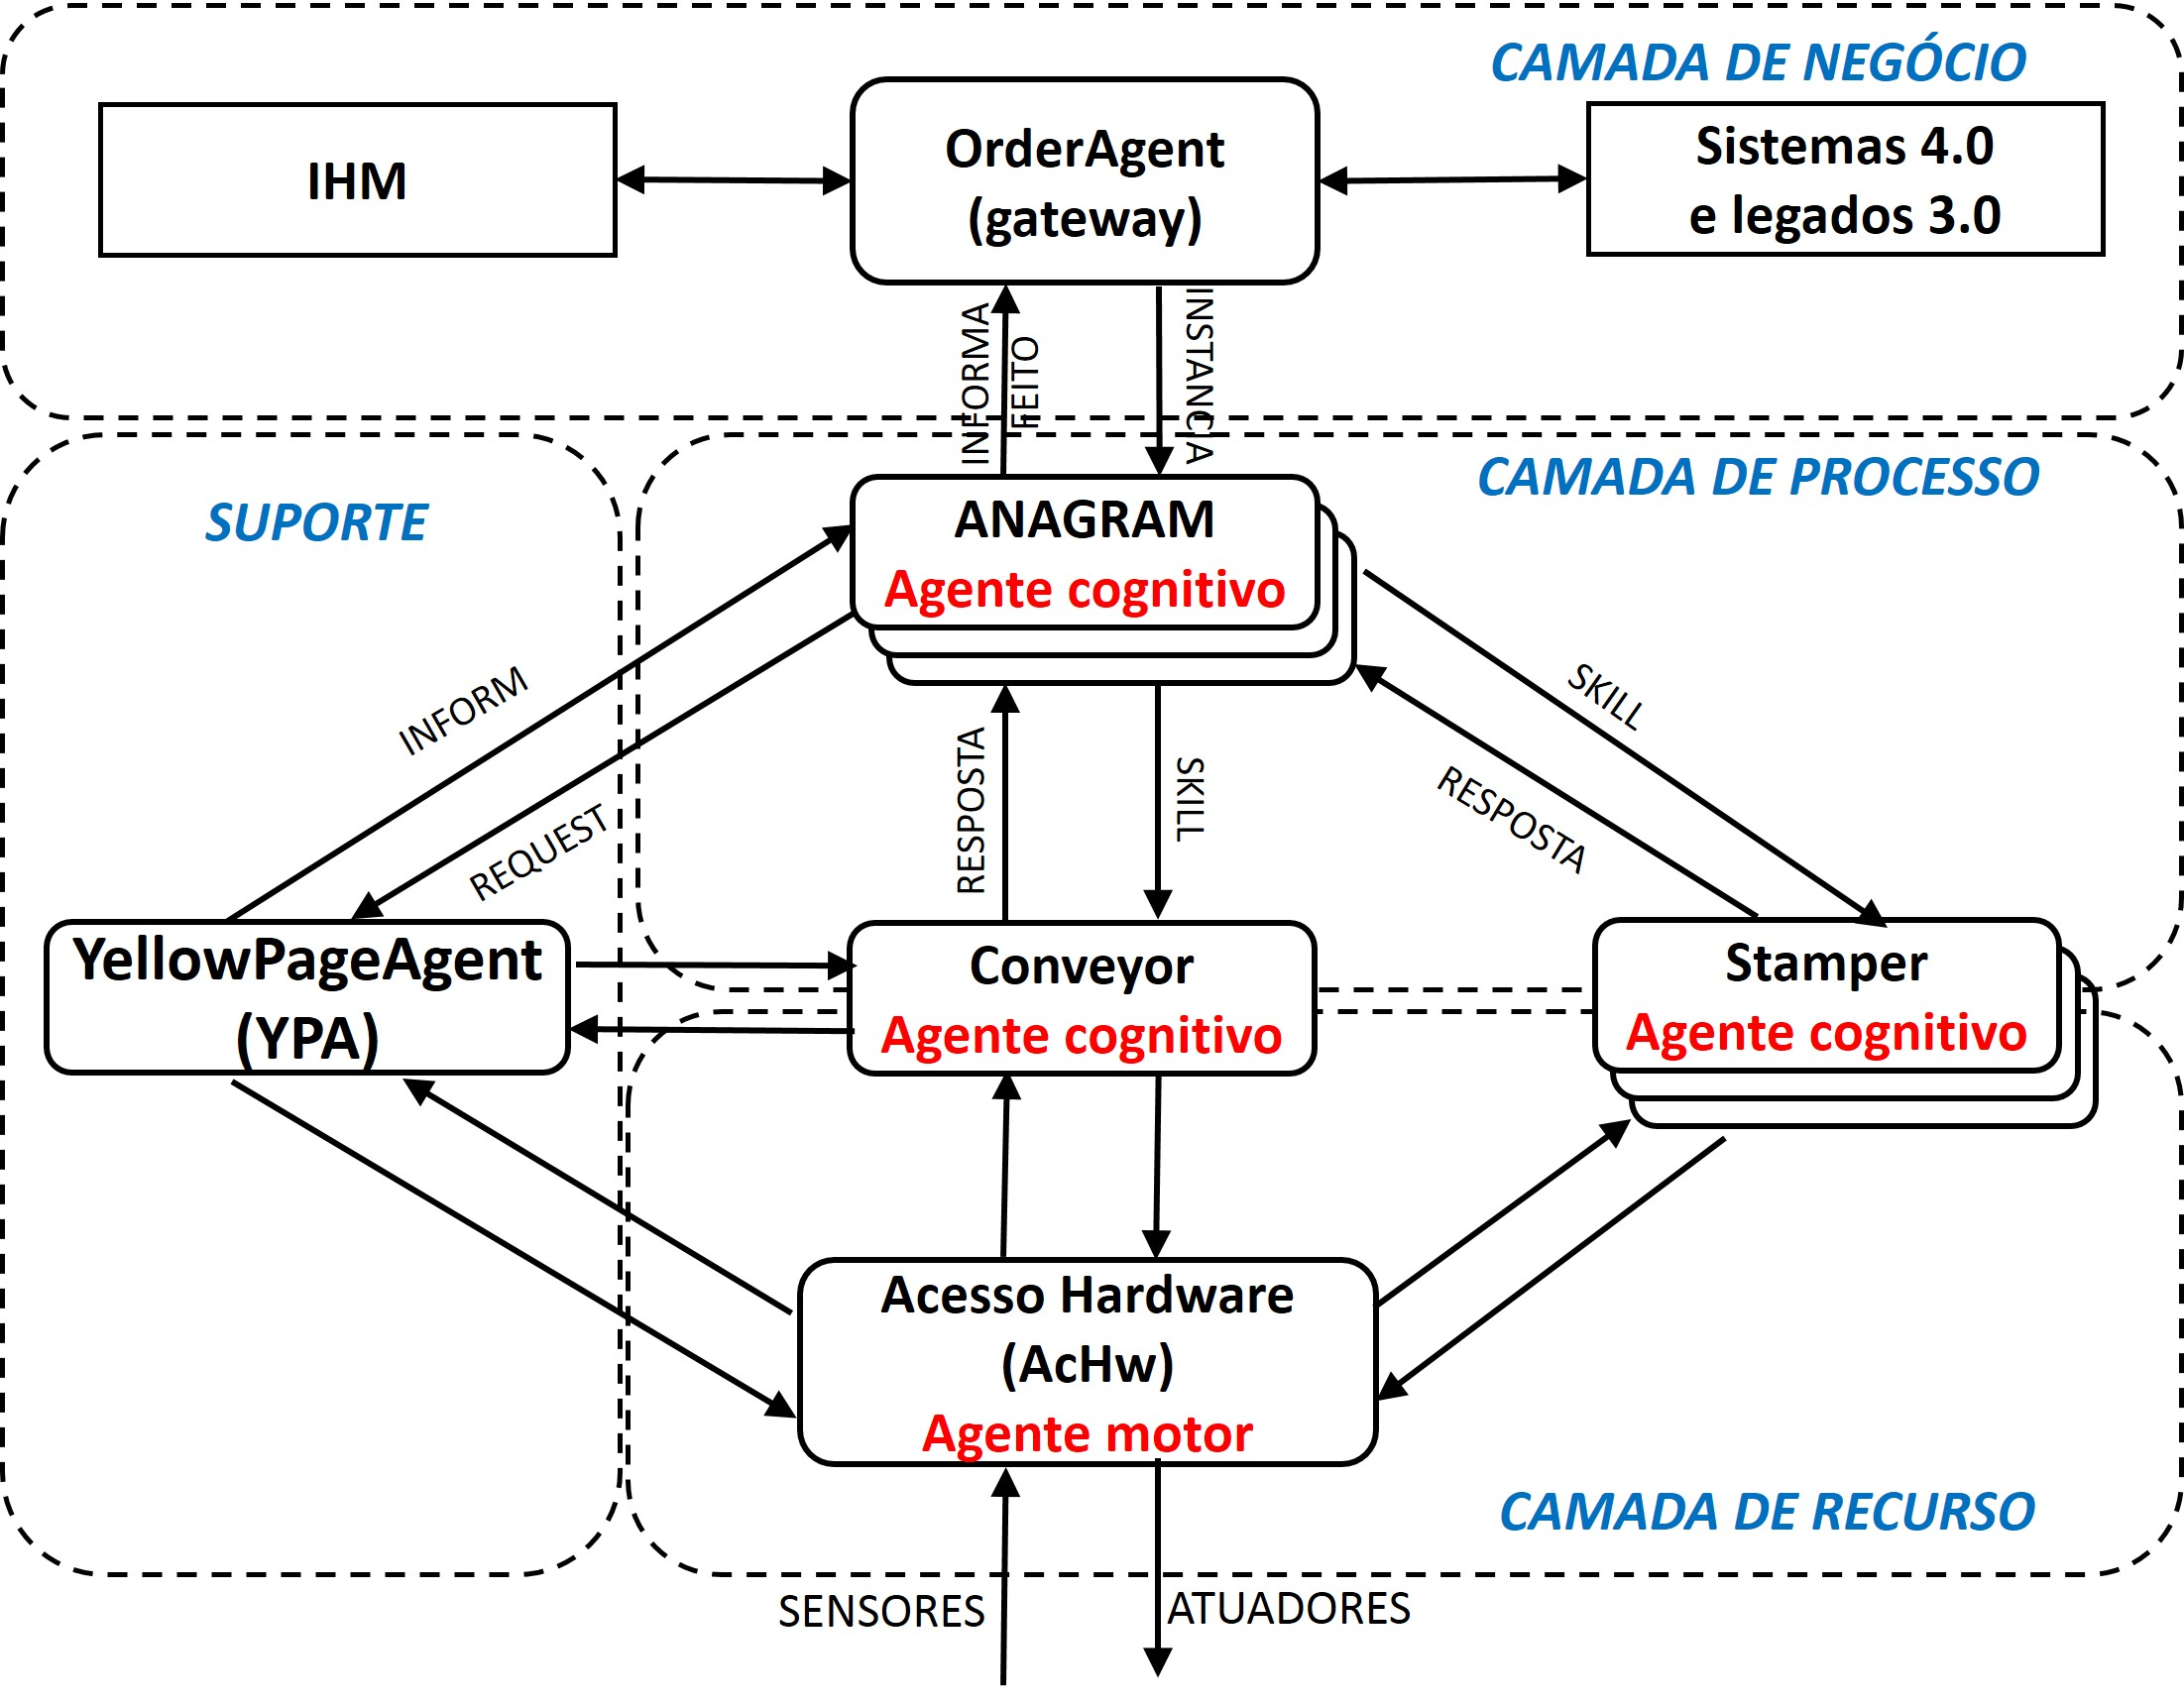
\includegraphics[width=0.8\textwidth ]{img/F140_SIAPE.jpg}
	\caption{Aplicação da arquitetura EPS no SIAPE}
	%\footnotesize{Fonte: O autor}
	\label{fig:eps_arquitetura_1}
\end{figure}

A principal contribuição do SIAPE  à arquitetura de Cavalcante é o reconhecimento da existência do agente \textit{OrderAgent}, na camanda de negócios, que é um tipo de agente que permite a comunicação externa com os agentes internos ao sistema, contudo não pode ser enquadrado como um agente cognitivo ou motor da arquitetura. A diferença reside no fato da função \textit{gateway} do agente de ordem de serviço permitir a comunicação com o operador, através da IHM, de uma forma transparente.

O agente Produto e o agente Recurso da arquitetura SIAPE, funcionam conceitualmente exatamente igual à arquitetura de Cavalcante, isto é, o agente cognitivo responsável pela lógica e inteligência do sistema e o agente motor fica responsável por receber as decisões do agente cognitivo e realizar as operações necessárias no processo produtivo.


%===================================================================

\section{Conceituação teórica de termos importantes para a pesquisa}	

O avanço da fronteira da ciência aproxima cada vez mais as áreas da Engenharia e da Computação. Neste contexto encontramos antigos termos combinados entre si para criar novos significados. O objetivo dessa seção é esclarecer o significado de alguns destes termos que são utilizados na sequência deste trabalho e evitar erros em suas interpretações.



\subsubsection{Auto-organização e emergência}

Sistemas EPS são dito auto-organizáveis e emergentes. 

Um sistema é chamado de auto-organizado quando é capaz de mudar a sua organização interna autonomamente, isto é, sem interferências externas, a fim de responder a uma mudança ambiental relevante. A \textbf{auto-organização} é, pois, a propriedade de um sistema de adquirir uma estrutura espacial, temporal ou funcional sem interferência externa. 

Há várias formas de se fazer tal auto-organização, por exemplo, através de um subsistema que detém toda a informação necessária para realizar a configuração do macro-sistema mediante uma análise cuidadosa do ambiente e das perturbações sofridas; esta é a solução centralizada. No entanto, quando o sistema não tem essa entidade centralizadora, pode ainda ser capaz de auto-organização quando os elementos que formam o sistema forem suficientemente inteligentes para se perceberem, interagirem e montarem a topologia mais adequada para a execução de um objetivo (ou múltiplos objetivos). Quando isto ocorre, é dito que o sistema é \textbf{emergente}, pois aparecem propriedades e padrões no nível macro, mas a informação de como tais padrões e propriedade devem ser formados não estão descritas \textit{claramente} nos elementos que formam o sistema. Diz-se que tais propriedades emergem da interação dos elementos constituintes do sistema. Do ponto de vista micro, as ações dos agentes são aleatórias, mas resultam em uma propriedade emergente no nível macro.

Um EPS possui auto-organização porque é capaz de autonomamente ajustar-se a variações na demanda, bem como reconhecer os elementos que o forma. Também é dito que possui \textbf{emergência} porque as interações entre os agentes ocorrem de forma dinâmica (não prevista), entretanto, um produto final é montado.

O período atual está sendo marcado pela busca de soluções para o problema recorrente da customização em massa. Esse período é, neste estudo, denominado de Indústria Híbrida devido ao fato da convergência de paradigmas, sistemas, arquiteturas e ferramentas na busca de uma solução ótima para o fenômeno da customização, sem no entanto se chegar a um denominador comum. 

Os sistemas evolutivos, com a aplicação de algumas de suas capacidades e propriedades, nesse caso, auto-organização e emergência, apontam para soluções eficazes, vencidas as complexidades, na busca de soluções definitivas para o problema recorrente da customização de massa.



\subsection{Plataforma da Indústria 4.0}	

O \textit{white paper} da Indústria 4.0~\cite{BITKOM2015} formulou as questões centrais da \iQuatroZero, a partir de um ponto de vista da pesquisa e inovação. Das recomendações publicadas, quatro são consideradas e descritas neste trabalho, conforme segue:

\begin{description}
	\item[A integração vertical (IVe)] -	
	é caracterizada pela capacidade dos sistemas integrarem os seus processos técnicos aos processos de negócio da empresa, para auxiliar no processo de decisão estratégica empresarial; uma das propriedades relacionadas é a interoperabilidade entre os sistemas; 
	
	\item[A integração horizontal (IHo)] -
	é a agregação, em tempo real~\cite{VDE2014} dos elementos de conhecimento que tais sistemas geram no chão--de--fábrica. Para isso relaciona-se a comunicação, o planejamento e a programação de tais sistemas, contendo elementos que serão usados para incorporar raciocínio baseado em casos de uso, evidenciando a capacidade de evoluir com a mudança dos requisitos de produção; 
	
	\item[A integração humana (IHu)] -
	é caracterizada pelo uso das capacidades de criação dos seres humanos considerados no desenvolvimento dos sistemas e na recuperação dos sistemas legados \iTresZero;
	
	\item[A engenharia 4.0 (E4.0)]
	é denotada pelos domínios dos conhecimentos de Engenharia durante todo o processo do ciclo de vida do produto, os quais o projetista deverá capturar com base na especificação do produto, desde a concepção ao encerramento do projeto, levando-se em conta as tarefas e habilidade dos agentes mecatrônicos do sistema. Inclui--se aqui o domínio da eletrônica, da mecânica, de software, das redes, entre outros;
\end{description}
	
A Indústria 4.0 representa a situação futura, entretanto, na atualidade, já estão sendo produzida as condições necessária ao seu funcionamento, a saber: os ciberespaços, contendo as ciberestruturas~\cite{NITRDGROUPS2010} os dispositivos e tecnologias que serão utilizados pela Indústria 4.0, que por sua vez, são baseados nos paradigmas evolutivos e nos (CPS)~\cite{LEE2008}. 

%Nesse contexto, a \textit{Internet of Things}~(IoT)~\cite{ROTONDI2013b} será obrigatória, e os grandes centros de tecnologias estarão, finalmente conectadas e interagindo entre os centros de referências de Ciência, Tecnologia e Inovação em torno do globo terrestre. 

Neste contexto, os grandes centros de desenvolvimento de C\&T\&I estão tomando iniciativas que visam a implantação da \iQuatroZero. Por exemplo, o Horizon 2020~\cite{H2020} é o maior Programa de Investigação e Inovação da UE. O programa já conta com cerca de 80 bilhões de euros em financiamento disponível ao longo de 7 anos (2014-2020), além do investimento privado que esse dinheiro vai atrair. Ele promete mais avanços, descobertas e estreias mundiais, possibilitando grandes ideias saírem do laboratório para o mercado. Visto como um meio de impulsionar o crescimento econômico e criar empregos na UE tem o apoio político dos líderes europeus e dos deputados do Parlamento Europeu. 
%Eles concordaram que a pesquisa é um investimento no futuro para o crescimento, o emprego inteligente, sustentável e inclusivo. 
	
%Quando a constante utilização de sistemas \textit{FMS} como solução para os lotes médios já não tinha a mesma eficácia, a personalização de produtos passou a ser tratado pela agilidade. Para isso os sistemas baseados em \textit{ FMS} foram substituídos pelos sistemas baseados nos paradigmas \textit{BMS, HMS e RMS}. No final desse período a agilidade teve sua eficácia reduzida como solução para o fenômeno da customização em massa e surge os sistemas emergentes baseados nos paradigmas \textit{EAS/EPS} e a auto-organização. \textit{A emergência aqui entendida como a propriedade de um sistema ser construído de forma determinística, por meio dos conceitos da auto-organização. A auto-organização, por sua vez é a propriedade de um sistema de adquirir uma estrutura espacial, temporal ou funcional sem interferência externa.}\par
	

\subsection{Termos do Sistema de Produção}	

No jargão do ambiente industrial, aparecem alguns termos que igualmente precisam ser aclarados. Neste trabalho, os seguintes termos terão os subsequentes significados:

%=====================================================================
\begin{figure*}
	\centering
	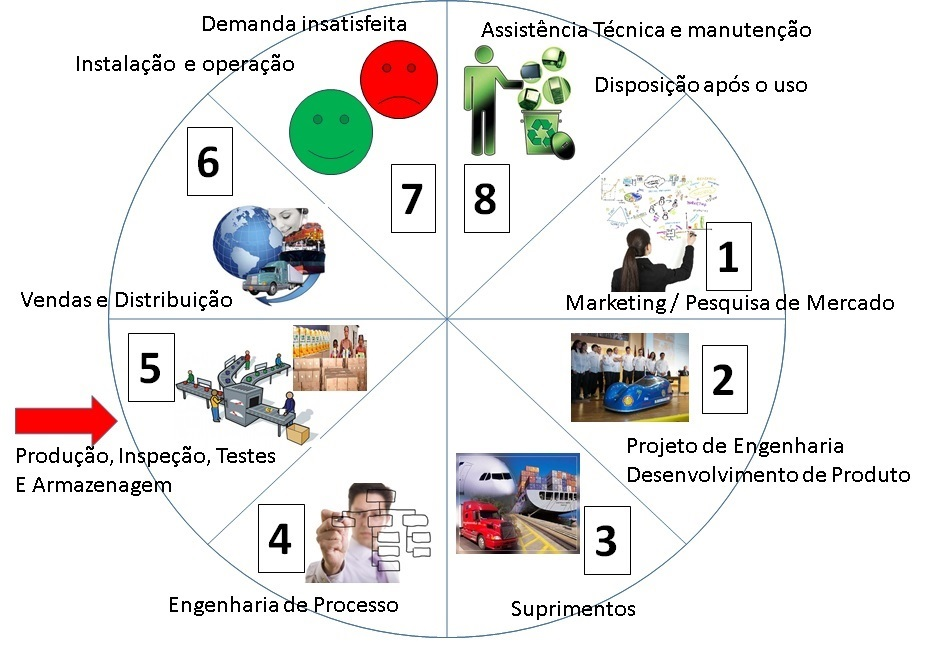
\includegraphics[width=0.8\textwidth]{img/F6_SIAPE_Ciclo_de_vida_do_Produto.jpg} 
	\caption{SIAPE: Ciclo de vida do produto}
	\label{F6}
\end{figure*}
%======================================================================
	
\begin{description}
	\item[Ciclo de vida do produto] -
	O ciclo de vida do produto descreve as fases do produto desde o seu nascimento até o seu descarte na sociedade. Tal ciclo é mostrado na Figura~\ref{F6}. Analisando a figura, tem-se o ciclo iniciado na fase 1, onde a equipe de marketing realiza pesquisas no mercado de demandas não atendidas (fase 7) para que esforços sejam aplicados nessa direção; na fase 2, a necessidade não atendida é transformada num produto a ser produzido; a fase 3, ilustra a compra e a logística dos insumos necessários para a realização do produto; na fase 4, a Engenharia de Processo prepara o produto para produzido em linhas de produção; a fase 5 acontece nas linhas de produção propriamente ditas, onde são efetivamente montados os produtos; na fase 6 o produto é vendido e distribuídos no comércio; a fase 7 ilustra o atendimento da demanda insatisfeita através do atendimento às necessidades do cliente; Na fase 8 tem-se a assistência técnica e a o posterior descarte após o uso do produto finalizado.
	
	\item[Reconfiguração ou tempo de \textit{setup} de linha de produção]
	Tempo de \textit{setup} é o período em que a produção é interrompida para que os equipamentos da linha de produção sejam ajustados, configurados ou reconfigurados. O tempo de setup está diretamente relacionado com as variações do produto e o planejamento da produção realizado pela indústria.
	Nos sistemas de produção em lotes, as paradas para ajustes estão mais presentes devido à necessidade de se produzir uma grande variedade de produtos, tornando o controle deste período uma necessidade crítica, fundamental para a garantia de uma boa produtividade. 
	
	\item[Configuração ou \textit{lead time} de linha de produção]
	É o tempo decorrido desde a concepção do produto até a montagem da linha e sua efetiva entrada em produção com toda a capacidade produtiva.
	
	\item[Curva de crescimento ou \textit{ramp up} de linha de produção]
	\textit{Ramp up} é um termo usado em economia e negócios para descrever um aumento firme na produção. Neste trabalho de pesquisa este termo está restrito à linha de produção.  Quando um plano de produção de um novo produto entra em linha, os recursos não conseguem atingir a quantidade ideal planejada e ajustes são realizados para que essas quantidades sejam alcançadas. O período entre o início da produção até que os recursos produtivos consigam atingir a quantidade planejada é definido como o \textit{ramp up}.
\end{description}

	
\begin{figure}[h!]
	\centering
	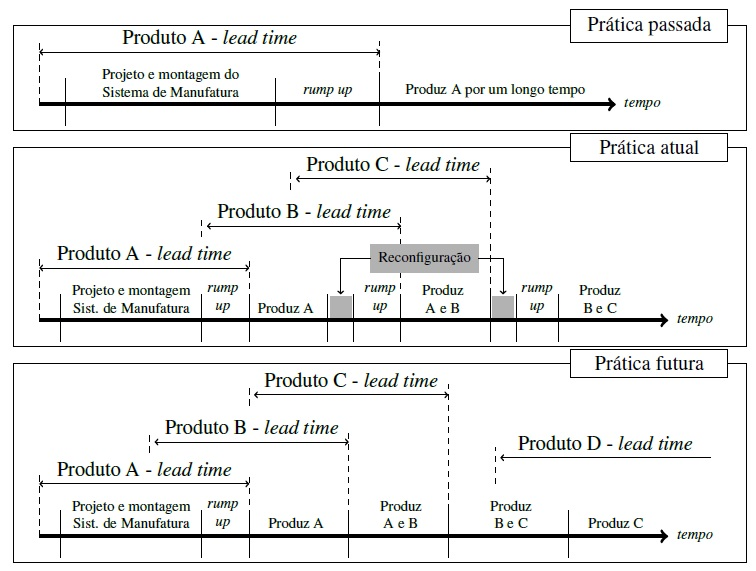
\includegraphics[width=\textwidth, height=10cm]{img/F8_SIAPE_Lead_Time_EPS.jpg} 
	\caption{Redução do Lead time de Produção}
	{\footnotesize{Fonte: \cite{KOREN1999} com adaptações de \cite{CAVALCANTE2012a}}}
	\label{F8}
\end{figure}
	

Com os volumes altos de produção, as configurações entre produtos eram realizadas em espaços de tempos que não preocupava o setor produtivo, entretanto tal não é mais a realidade atual. A Figura~\ref{F8} descreve esse processo onde pode ser evidenciado que o produto A, na prática passada de manufatura, produz durante um longo período de tempo, enquanto que atualmente, convivem vários produtos (A,B,C) simultaneamente em produção. Mais ainda, vislumbra-se que a prática futura exija que um tempo de reconfiguração e as paradas de linha tendam a zero.




\subsection{Agentes e Sistemas Multi-Agentes (MAS)}	

O termo \textbf{agente} continua sem uma definição universalmente aceita, existindo  ainda muito debate e controvérsias, contudo para nortear este trabalho, o termo agente foi conceituado como uma entidade abstrata que age no mundo real por meio de sensores que percebem o ambiente e atuadores que alteram esse ambiente para atingir metas estabelecidas. Esse conceito tem suas bases nas seguintes definições:\par 

\begin{quote}
	\textit{``Um agente é algo capaz de perceber seu ambiente por meio de sensores e de agir sobre esse ambiente por meio de atuadores''} \cite{Russell_Norvig1995}.
\end{quote}

\begin{quote}
	\textit{``Um agente é um sistema de computador que está situada em algum meio, e que é capaz de agir autonomamente neste ambiente, a fim de atender seus objetivos de projeto''} \cite{WOOLDRIDGE2002,WOOLDRIDGE2007}
\end{quote}

Agentes conseguem perceber o ambiente e agir sobre ele para alterá-lo. Dentre as diversas características de agentes, neste trabalho foram enfatizadas as seguintes: 

\begin{enumerate}
	\item Autonomia - agentes atuam cumprindo seus objetivos individuais; 
	
	\item Sociabilidade - agentes interagem entre si estabelecimento uma sociedade de agentes; 
	
	\item Racionalidade - um agente pode raciocinar sobre os dados que ele recebe, através de seus sensores ou de comunicação com outros agentes, a fim de encontrar a melhor solução para atingir o seu objetivo; 
	
	\item Reatividade - um agente pode reagir à mudanças no seu meio ambiente; 
	
	\item Pró-atividade - um agente pode ativamente agir no seu meio buscando os seus objetivos;
	
	\item Adaptabilidade - um agente é capaz de aprender e mudar seu comportamento quando uma solução melhor é descoberta. 
\end{enumerate}

Um sistema formado por agentes de diferentes tipos, ou vários agentes de um único tipo, que interagem entre si, formam um sistema multiagente (MAS). Tais sistemas são por natureza descentralizados e modulares, facilmente adaptáveis ao meio e capazes de resolver problemas complexos. 

Agentes são particularmente interessantes para os paradigmas industriais emergentes, pois estes são modulares, descentralizados, e necessitam de adaptação. Utilizando-se MAS nos sistemas evolutivos implica num ambiente de resiliência, sustentabilidade, robustez, tolerância a faltas~\cite{RIBEIRO2013a}. EPS é baseado em agentes. 

\subsection{O protocolo \textit{FIPA -- Foundation for Intelligent Physical Agents}}	

A \textit{FIPA (Foundation for Intelligent Physical Agents)} é uma associação internacional de companhias e organizações que juntas unem esforços a fim de produzir especificações para tecnologias de agentes que sejam aceitas de uma forma genérica. A FIPA promove um conjunto de tecnologias para diferentes áreas através de um conjunto de documentos que  definiram as regras que permitem a uma sociedade de agente existir, operar e ser gerenciada.  Dentre esses documentos encontram-se as especificações \textit{FIPA--ACL (Agent Communication Language)} que definem a comunicação entre os agentes. 

A Figura \ref{F93} ilustra os protocolos responsáveis pelo mecanismo de negociação e execução de funcionalidades dentro dos protocolos. A parte \textit{a} da figura mostra o Protocolo \textit{FIPA Request Interation Protocol} e a parte \textit{b} mostra o FIPA Contract Net Interation Protocol. Para este trabalho, o \textit{FIPA Request Interation Protocol} atinge os objetivos almejados.

Dentre os campos constantes nos campo definidos nas mensagens FIPA, os seguintes campos podem ser encontrados: 1) A Identificação do agente no sistema (AID); 2) O Conteúdo das mensagens expressas por caracteres; 3) O controle de mensagens, expresso pela identificação da conversa, o tipo de mensagem, tempo máximo, entre outros; 4)Ontologia, responsável pelo significado dos termos dentro do contexto de trocas das mensagens.


\begin{figure}
	\centering
	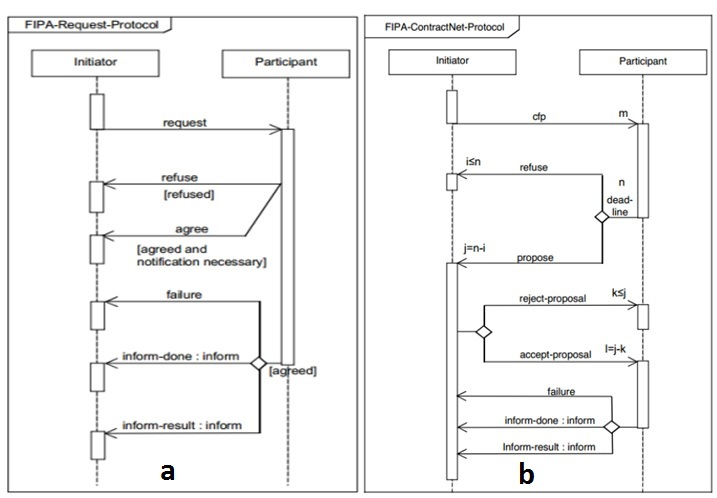
\includegraphics[width=16cm, height=10cm]{F93_SIAPE_FIPA.jpg}
	\caption{SIAPE: FIPA -- ACL}
	\footnotesize{Fonte:~\cite{FIPA2002b,FIPA2002c}}
	\label{F93}
\end{figure}		


\section{As Fases do Paradigma Evolutivo: acadêmica, experimental e holística}

Na Figura~\ref{F11} visualiza-se onde EPS está colocado, em termos históricos, no conjunto dos paradigmas da manufatura. Para uma análise específica das pesquisas realizadas em EPS, dividiu-se estes estudos em três fases distintas, a saber:


%==============================================================
\begin{figure*}[h]
	\centering
	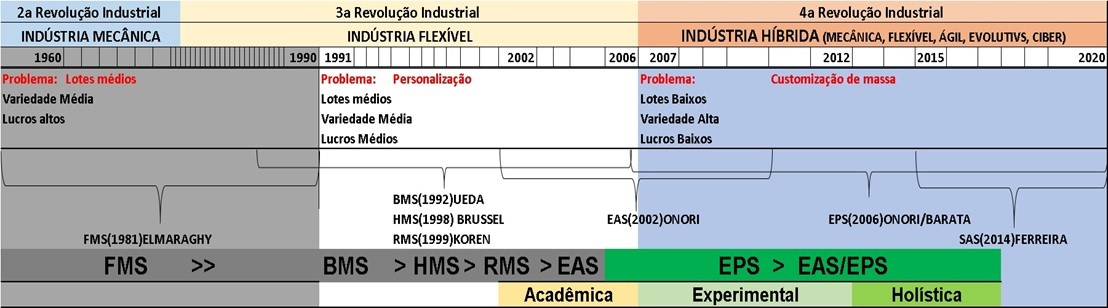
\includegraphics[width=\textwidth, height=6cm]{img/F11_SIAPE_Fases_EPS.jpg} 
	\caption{MeDSE - Fases do paradigma EPS}
	%\footnotesize{Fonte: Adaptado de~\cite{MUNZLINGER2012,MONTEBELO2000,SAMPAIO2007}}
	\label{F11}
	
\end{figure*}
%==============================================================

\begin{enumerate}
	\item A Fase Acadêmica: encontraram-se as pesquisas conceituais, simulações e primeiras provas de conceitos. Essa fase foi identificada entre os anos de 2002 quando surge a base dos sistemas evolutivos, o paradigma EAS e se estende até 2006 quando Onori estabelece as bases do paradigma \textit{EPS};
	
	\item  A Fase Experimental: onde o paradigma toma dimensões de testes e experimentos realizados por vários pesquisadores e dura até a prova de conceito do Projeto \textit{IDEAS} em 2012;
	
	\item  A Fase Holística: o paradigma percebe na prática a complexidade gerada pela interdisciplinariedade, e nesse momento, o foco foi além do chão-de-fábrica e transcendeu os campos Engenharia e da Computação para o campo da Economia, dos Sistemas complexos, da Inteligência Artificial, da Biologia e outros campos do conhecimento humano. 
\end{enumerate}


\subsection{A Fase Acadêmica do Paradigma Evolutivo}

Para encarar de frente o problema da personalização, foram criados os paradigmas \textit{BMS} utilizando seus \textit{modelons}, o \textit{HMS} com a ideia de \textit{holons} e o \textit{RMS} que, através da reconfiguração, consegue tratar as mudanças ambientais relevantes.

Na impossibilidade de solução ótima, pois cada tipo de sistema apresenta suas particularidades e desafios próprios, inicia-se a Fase Acadêmica do paradigma \textit{EPS}, no início do século XXI. Com o surgimento do paradigma \textit{EAS}, que utiliza das tecnologias de agentes e avanços no campo das linguagens de programação, modelagem e redes, \cite{ONORI2002} expandiram estes conceitos e os aplicaram na manufatura. EAS/EPS, usam módulos inteligentes, que comunicam-se em rede, através dos protocolos FIPA \cite{FIPA2013}, e princípios de Inteligência Artificial (IA) \cite{Russell_Norvig1995}. Realizam os conceitos da plugabilidade (\textit{plug and produce}) através da auto-organização e emergência de agentes.

O trabalho desenvolvido por \cite{BARATA2003} denotou uma arquitetura de referência para avaliar a questão da agilidade no chão de fábrica, e assim dominar as perturbações e incertezas do mercado que atingia o sistema. A composição do sistema e o seu comportamento são estabelecidas através da configuração das relações entre os módulos, usando mecanismos contratuais. A elevada capacidade de reutilização era motivada pelo conceito de módulos que eram facilmente atualizados para posterior reutilização. 

%As interações eram realizadas por módulos de fabricação e as coalizões regidas por contratos que eram configurados sempre que uma coalizão estivesse estabelecida. 



%=============================================================

\subsection{A Fase Experimental do Paradigma Evolutivo}

Em 2007 o trabalho conjunto de \cite{FREI2007} analisa o contexto e implicações do novo paradigma de produção \textit{EPS}.  Neste trabalho Frei reconhece a agilidade, a sustentabilidade e a reatividade como pontos chaves para tratar problemas de sistemas dinâmicos. Os sistemas evolutivos tendem para a solução do problema da customização, no entanto, precisam ser mais amadurecidos e tornados mais robustos para lidar com os distúrbios dos mercados atuais, e para isso, o paradigma \textit{EPS} tem sido evoluído e atualizado o suficiente para realizar essa tarefa.

O trabalho de \cite{MAFFEI2009} apresenta uma versão simplificada do paradigma \textit{EPS}, em uma forma de metodologia, que permitiu que o conceito de ciclo de vida de um produto e as ferramentas de avaliação de investimento puderam ser integrados. O trabalho identificou, entre outras coisas, as conquistas atuais dentro dos estudos do paradigma EPS que possibilitam às empresas relacionar requisitos de suas necessidade com algumas características de um modelo de negócio aplicável ao modelo atual de desenvolvimento de produto baseado em EPS.

\cite{CANDIDO2011} apresentaram a associação de \textit{EPS} com a abordagem \textit{Service Oriented Architectures} (SOA), na  busca de um objetivo comum, a nível do dispositivo para o domínio da automação industrial, delineando princípios arquitetônicos fundamentais e de um modelo de dispositivo para apoiá-lo. A associação entre SOA e EPS foi demonstrada através de um protótipo que confirmou a sua aplicabilidade num cenário esperado de caso de uso em automação industrial.

\cite{CAVALCANTE2012a} trazem uma visão geral dos paradigmas de manufatura, realiza uma breve descrição das pesquisas em torno do tema EPS e lança as bases para criação de uma linha de montagem que assimile os conceitos, tecnologias e paradigmas evolutivos que podem ajudar o Brasil nos avanços para a $4^a$ Revolução Industrial.

Por outro lado, \cite{AlGeddawy2012} apresentam o modelo para prever o futuro desenvolvimento de novos produtos e sistemas de manufatura. O modelo é inspirado no sistema biológico aplicado aos recursos de produção para prever potenciais alterações nas condições comportamentais do sistema. Uma técnica matemática é aplicada para gerar uma síntese de conhecimento de co-evolução e analisar as relações entre as capacidades de fabricação e as características do produto. Regras são previamente estabelecidas e um sistema de equações lineares é formulado para descobrir o movimento das potenciais alterações nos sistemas.

Também neste ano, \cite{RIBEIRO2012b} publicam aplicações de Inteligência Artificial que utilizam os modelos de cadeia ocultas de Markov para realizar as análises estocásticas das respostas dos sistemas. Com as respostas em mãos, as correções de erro são trabalhadas para corrigir as variações dos sistemas e fazê-los responder com robustez às perturbações~\cite{RIBEIRO2012b,RIBEIRO2012a}; e \cite{CAVALCANTE2012} propõe sua arquitetura baseada em agentes que realiza auto-organização, mas também permite auto-otimização em alguns dos recursos do sistema. Em sua arquitetura usa a noção de \textit{skills}, descoberta de serviços e auto-organização de agentes, e foca nas questões mais relevantes do problema da customização no chão de fábrica com o objetivo do \textit{plug and produce}.


%===============================================================
\subsection{A Fase Holística do Paradigma Evolutivo}

Nos anos de 2013 e 2014 percebe-se uma acentuada elevação nas pesquisas em torno dos sistemas \textit{EAS} e \textit{EPS}. Agora, de uma forma mais qualitativa, os pesquisadores se valem de novos conceitos, técnicas, teorias e avanços tecnológicos para realizarem, na prática, as pesquisas que foram concluídas com sistemas demonstradores. 

Esta fase começa com \cite{ROSA2013c} que apresenta sua arquitetura na forma de um \textit{framework} probabilístico no paradigma EAS/EPS utilizando-se sistemas multiagentes. Rosa afirma que existe uma falta de métricas para o estudo dos sistemas que exploram os conceitos da auto-organização e respostas autônomas. Seu principal objetivo foi trabalhar com pequenos sistemas que utilizem pequenos volumes de produção de produtos com elevada variabilidade.

Já os trabalhos de \cite{MAFFEI2013, MAFFEI2013j}vai além do chão de fábrica para desenvolver um sistema que caracteriza os custos e cria estratégias de automação em ambientes que utilizam sistemas evolutivos de produção. O trabalho traz uma abordagem holística, contudo, percebe-se que a efetivação do paradigma EPS nos vários níveis das empresas ainda precisa de muita implementação.

\cite{Akillioglu2013} trazem, para o campo da investigação, mais uma questão que faz uma abordagem holística do paradigma EPS, utilizado o conceito de demanda responsiva, denotada como um tipo de planejamento ágil. %A questão é relevante porque é investigada por pesquisadores que tem \textit{know-how} neste tipo de assunto, podendo assim ter avanços significativos para sistemas evolutivos.

\cite{NEVES2013} apresentam uma arquitetura chamada de \textit{Adaptador} com uma arquitetura genérica que suporta projetos e prospecções de métodos, que servem para suporte de projetos e para a configuração de sistemas mecatrônicos. O projeto se assemelha à modularização e empacotamento de objetos numa abordagem orientada a objetos.

\cite{RIBEIRO2013} chamam a atenção para os estudiosos que não estão aplicando corretamente os conceitos e ferramentas para realizarem os sistemas baseados nos vários paradigmas. Eles fazem uma revisão nos paradigmas e avanços para explicar a correta aplicação, inclusive com exemplos. O artigo deixa claro que os desempenhos dos paradigmas, incluindo \textit{EAS/EPS}, não estão correspondendo às expectativas, contudo, os autores atribuem essa dificuldade aos estudiosos e pesquisadores que não aplicam corretamente os procedimentos para uma perfeita atuação das propriedades dos sistemas. Para que haja uma melhor compreensão, um novo conjunto de ferramentas e perspectivas são necessárias e devem refletir os implicações e lógica da auto-organização e da emergência em um contexto de mecatrônica.

\cite{ROCHA2014} apresentam algumas mudanças arquitetônicas em relação ao EPS tradicional e as justificam em uma análise de controle da auto-organização. Os autores voltam ao tema da personalização em massa, explicando a implicação de que o sistema de produção tem que ser extremamente dinâmico ao tratar com o problema do lote de produção, pois a capacidade de reconfigurar rapidamente o sistema é primordial. Isso envolve tanto as estações que realizam processos de produção quanto o sistema de transportes. Segundo os autores, tradicionalmente, questões de reconfiguração de sistema são abordados a partir de um ponto de vista da otimização, implicando que a alocação de um determinado lote de trabalho para máquinas/estações específicas em um cronograma seja ideal. Contudo, o número e a natureza dos seus pressupostos de base são irreais, dado que mesmo uma quantidade pequena de elementos na produção pode gerar uma quantidade enorme de alternativas, não permitindo o uso dos algoritmos em tempo de produção. Aplicando-se a auto-organização ao problema, contudo, tem-se a vantagem de se alcançar uma solução justa, em um ambiente concreto e como uma reação das condições operacionais atuais. Mesmo que não possa ser realmente asseguradas as condições ótimas, as soluções atingem os reajustamentos online e tornam o sistema mais robusto.

É lugar comum entre as pesquisas que o problema de customização de massa ainda é o problema da indústria de transformação do século XXI, e que este problema, segundo as análises apresentadas neste estudo será conseguido com as propriedades presentes nos sistemas evolutivos: resiliência, auto-organização, auto-otimização, escalabilidade, e interoperabilidade.

Os sistemas evolutivos por seu turno denotam na atualidade o que existe de mais promissor para enfrentar o problema da customização, contudo, as tecnologias e ferramentas devem estar num estágio de maturidade ainda não alcançado. Para isso é necessária a utilização, preparação e especialização de ferramentas refinadas no campo. Os desafios são grandes, devido a interdisciplinariedade e complexidade das teorias e demandam pesquisas nas mesmas proporções.

%======================================================



\chapter{Desenvolvimento}
\label{cap:desenvolvimento}

Este capítulo descreve o desenvolvimento do  Sistema Inteligente Ágil de Processo Evolutivo - SIAPE, o qual segue o paradigma EPS. Para este desenvolvimento foi criado um método de desenvolvimento em que os princípios de EPS foram usados desde as fases mais primordiais do desenvolvimento. O método de desenvolvimento criado foi chamado de Método de Desenvolvimento de Sistemas Evolutivos - MeDSE. Duas seções foram utilizadas para realizar essa descrição: 

Na Seção 3.1 são descritas as três fases do método de desenvolvimento, a saber: Fase de Conceitos, Fase de Realizações e Fase de Finalizações. A seu turno, cada fase é composta por um número parcial de etapas, de um total de dez, que facilitam o desenvolvimento de cada fase.

A Seção 3.2 descreve a aplicação do método de desenvolvimento no protótipo SIAPE por meio das descrições dos desenvolvimentos de suas partes mecânica (descrição dos dispositivos definidos para a parte mecânica), eletrônica (a descrição dos circuitos elétricos), de software (descrição dos agentes mecatrônicos e seus \textit{skills})  e comunicação (descrição dos protocolos \textit{FIPA} utilizados na comunicação entre os agentes mecatrônicos do sistema) e suas  integrações.


%================================ VISÃO GERAL DO MEDSE =================================

\section{Visão do Método de Desenvolvimento de Sistemas Evolutivos (MeDSE)}

Para realizar o desenvolvimento do (SIAPE) identificou-se a necessidade da criação de um método que contemplasse a noção de agentes inteligentes e suas habilidades, que são denominados de \textit{skills} no paradigma \textit{EPS}, desde as primeiras fases do desenvolvimento. O método foi denominado de Método de Desenvolvimento de Processo Evolutivo (MeDSE). 

\begin{landscape}
 	\begin{figure}[h]
  		\centering
 		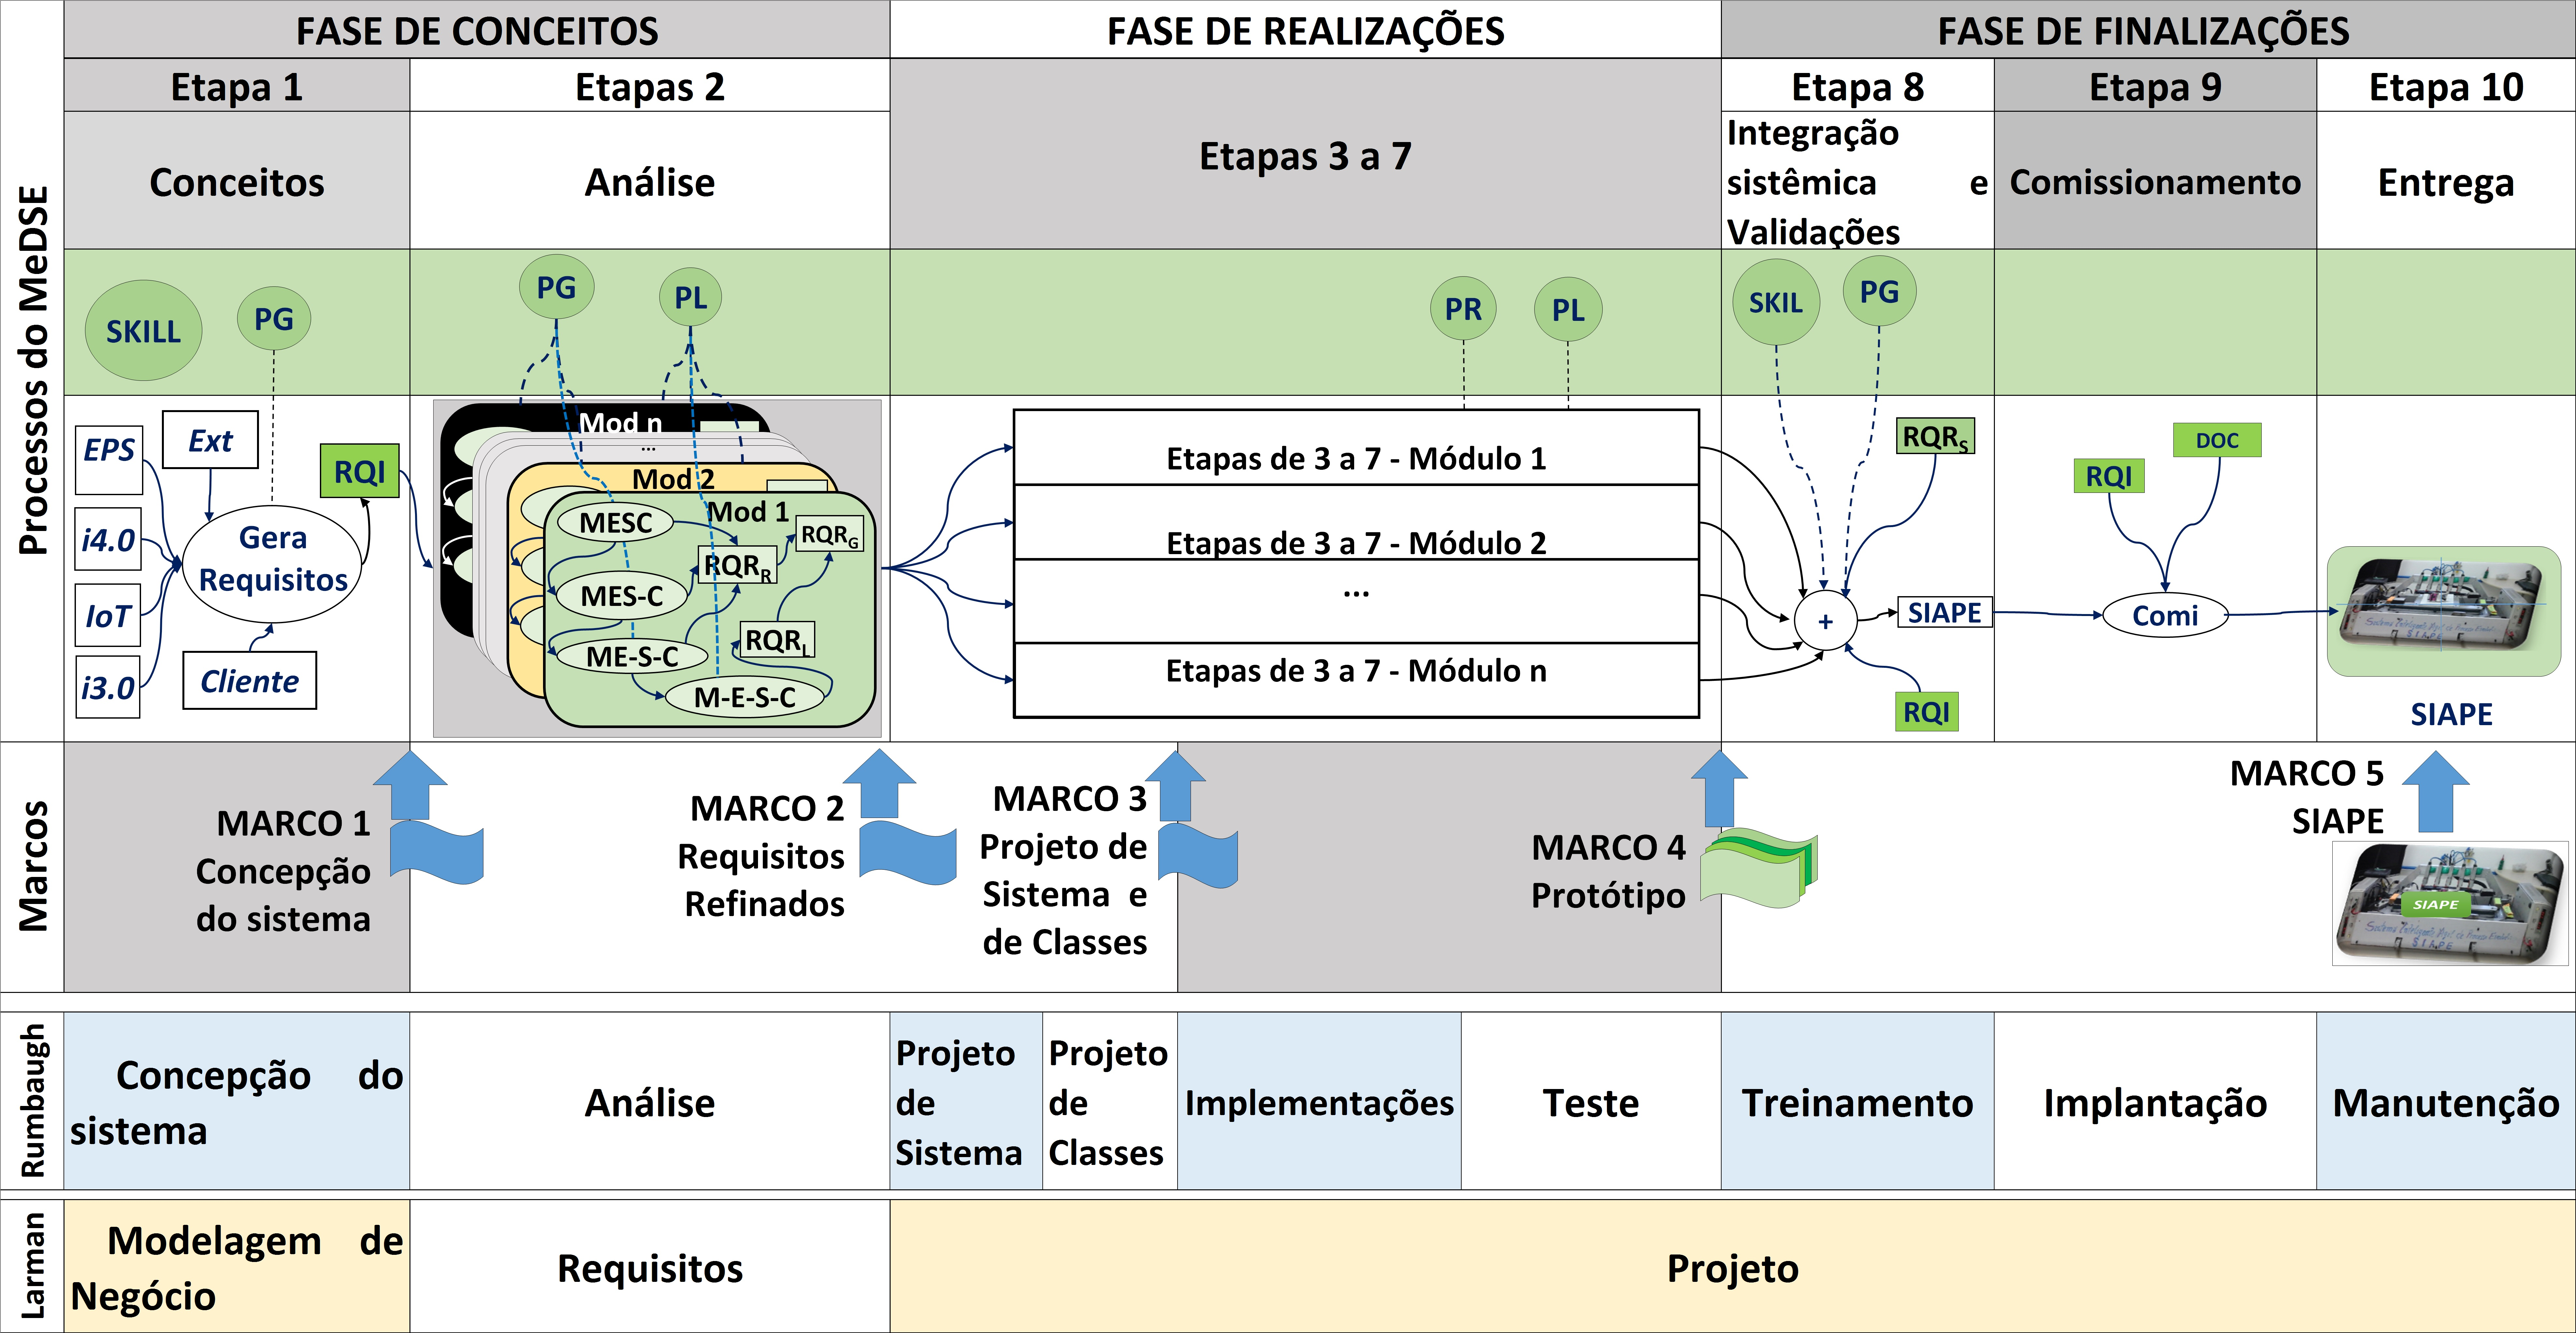
\includegraphics[width=20cm, height=14cm]{F25_SIAPE_VISAO8_1.jpg} 
 		\caption{Método de Desenvolvimento de Sistemas Evolutivos - MeDSE}
 		\label{F13_1}
 	\end{figure}
\end{landscape}
 
Depois de criado, o método foi comparado aos métodos utilizados por \citeonline{RUMBAUGH2006} e \citeonline{LARMAN2007}. A comparação com \citeauthor{RUMBAUGH2006} teve como principal objetivo a criação dos marcos do MeDSE. \textit{LARMAN 2007} foi utilizado para melhorar a acurácia na definição de requisitos e seus refinamentos. 
A Figura~\ref{F13_1} ilustra a visão geral do MeDSE na qual pode-se identificar as fases, as etapas, as atividades e os marcos a partir dos métodos comparados. Tais itens são explorado nas subseções seguintes.


\subsection{Definição de agente mecatrônico, problema global, problema regional e problema local}

Uma parte importante do MeDSE são os conceitos de Problema Global (PG), Problema Regional (PR) e Problema Local (PL).


A Figura \ref{F15}, mostra um esquema de como tais conceitos se relacionam. Nesta figura:
\begin{description}
	\item[M] - denota uma parte mecânica
	\item [E] - denota uma parte eletrônica
	\item  [S] - denota a parte de software
	\item  [C] - denota a parte de comunicação
	\item  [ME/MES/MESC] - Algum conjunto destas letras - corresponde a uma visão integrada daquelas partes. Ex.: ME é a integração entre a parte mecânica e a parte eletrônica.
	\item  [Cp] - é um componente composto, por exemplo, o SIAPE é uma composição de vários MESC.
	\item  [At] - é um componente visto de forma atômica. Ex.: a parte mecânica pode ser projetada de forma independente, segundo suas propriedades mecânicas, em relação às outras partes do sistema/subsistema/módulo.
	\item  [?] - denota um outro componente que pode ser qualquer um dos aqui discutidos.
	\item  [Propriedades] - uma ou mais característica, ou propriedade, ou atributos da entidade ou do sistema.
	\item  [Triângulo] - representa uma integração (composição) se vista de baixo para cima ou uma especialização (decomposição) vista de cima para baixo no diagrama.
\end{description}


\begin{figure}
	\centering
	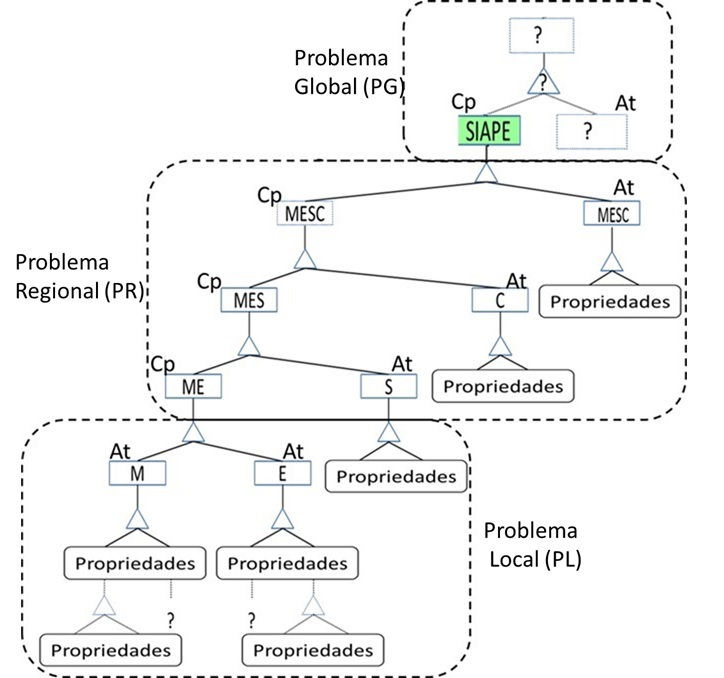
\includegraphics[width=10cm,height=8cm]{F15_PG_L.jpg} 
	\caption{MeDSE: Dividindo o problema global em regional e local}
	\label{F15}
\end{figure}

\begin{description}
	
\item[Definição de agente mecatrônico] - Neste trabalho, os agentes mecatrônicos são os módulos do sistema de manufatura e são identificados pela sigla MESC (Mecânica, Eletrônica, Software, Comunicação), indicando um sistema/subsistema/módulo completamente funcional.

Na Figura 3.2, um ou mais destes módulos serão integrados no sistema SIAPE.

\item[Definição de problema global (PG)] - Problema global é definido como a identificação do sistema como um todo e todas as partes a serem envolvidas. Essa identificação deve representar o consenso entre os especialistas da parte do cliente e a equipe de desenvolvimento. Por exemplo, um carro acoplado a um motor elétrico é integrado a um controlador, o qual contém um software que tem a capacidade de acelerar e parar o carro conforme ordens vindas pela rede. A Figura~\ref{F15} corresponde ao SIAPE.


\item[Definição de problema regional (PR)] - Problema regional é definido como uma visão do sistema na qual os relacionamentos entre as partes que o formam dependem funcionalmente uma das outras. Na Figura 3.2, por exemplo, ME e MES correspondem a dois problemas regionais. ME contém atributos/propriedades tanto mecânicos quanto eletrônicos, que formam então uma entidade de nível mais alto, integrada. MES, por outro lado, contém atributos/propriedades mecânicas, eletrônicas e de software. Formam uma entidade de nível ainda mais alto, quase um módulo completo.
Já MESC é outro problema regional e que denota um módulo completo, um agente mecatrônico.

\item[Definição de problema local (PL)] - Problema Local é definido como a visão em que as entidades que formam o sistema são atômicas, isto é, podem ser analisadas e desenvolvidas sem interferência de outras entidades. Na Figura~\ref{F15}, as entidades M e E, que correspondem aos conjuntos Mecânicos e Eletrônicos, podem ser analisadas individualmente com seus atributos e propriedades eletrônicas e mecânicas separadamente. Por exemplo: no conjunto mecânico, uma especificação possível pode aparecer como: um carro deve movimentar-se sobre um trilho; tanto a largura do carro e a bitola do trilho são especificadas sem nenhuma influência da parte eletrônica e podem ser analisados pela equipe mecânica sem restrições. O motor que faz o carro funcionar, pode igualmente ser especificado em termos de torque e velocidade mecânicos, mas a equipe eletrônica pode fazer análise de seu funcionamento independentemente da mecânica.\par 

Ainda analisando a Figura \ref{F15} pode-se perceber que as entidades M e E não conseguem mais ser decompostas em outras entidades, pois encontram-se em suas formas atômicas. Quando uma entidade atinge a sua forma atômica, o projetista chegou ao nível ideal para realizar a modelagem da entidade, pois em sua forma atômica, a entidade não sofre interferências de outra entidade externa. A tentativa de decompor a entidade levará ao nível das propriedades da entidade decomposta, ou seja, levará à desestruturação da mesma, inviabilizando o processo de modelagem. \par  

\end{description}


\subsection{A Fase de Conceitos}
  
A Fase de Conceitos corresponde  à realização conceitual, isto é, a concepção do sistema e a definições dos requisitos conforme \citeonline{RUMBAUGH2006} e \citeonline{LARMAN2007}. O objetivo dessa fase é estabelecer uma visão comum entre as equipes de desenvolvimento e os representantes do cliente e o escopo básico do projeto. Seus procedimentos partem da consideração de que existe um problema global que deve ser subdividido em problemas menores para serem tratados atomicamente até se tornarem requisitos que são modelados e simulados para que possam garantir a definição das especificações das partes do sistema.
 
Essa fase é composta por duas etapas ilustrada na Figura \ref{F27_1} e são descritas nas próximas subseções.
 
\begin{figure}[h]
 	\centering
 	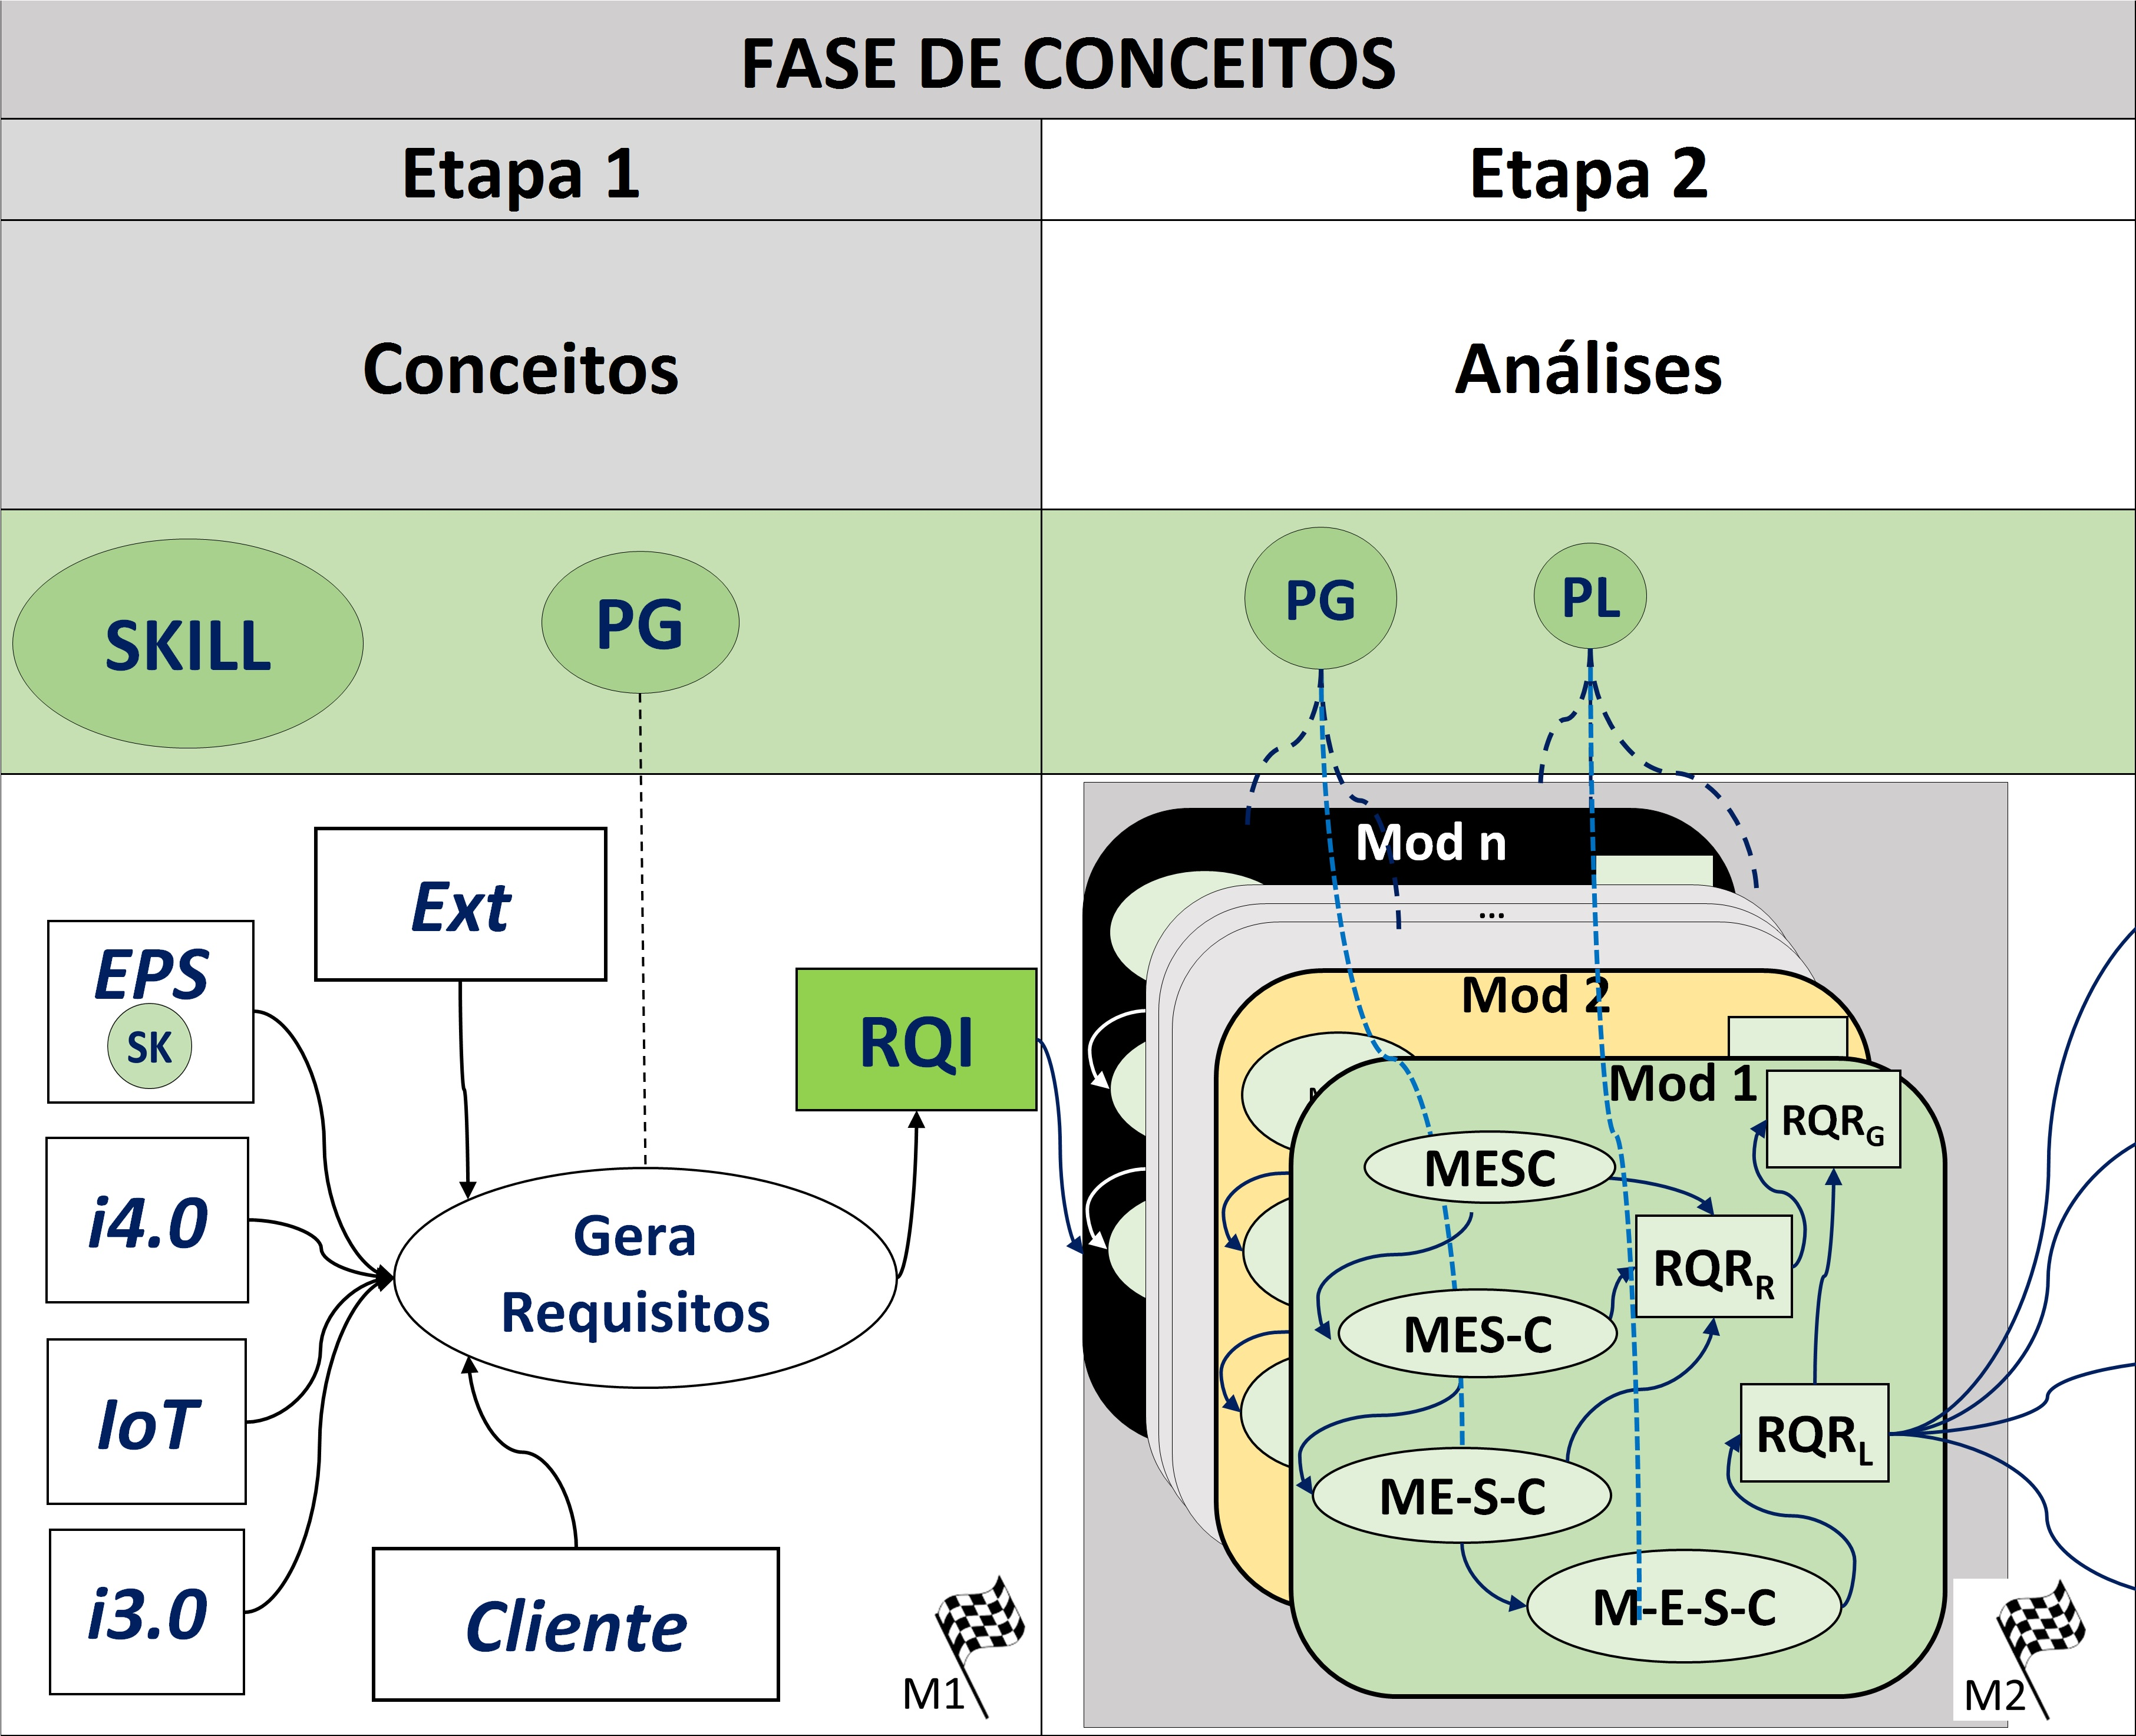
\includegraphics[width=10cm, height=5cm]{F27__SIAPE_FASE1.jpg} 
 	\caption{MeDSE: Fase de Conceitos}
 	\label{F27_1}
\end{figure}
 
\begin{description}
 	 \item[Etapa 1 - Conceitos] - A Etapa 1 tem como entrada as informações relativas ao sistema e as necessidades do cliente e sua saída é um documento de definição da concepção do sistema que contém os Requisitos Iniciais (RQI). Além da concepção do sistema, que deve ser aprovado por ambas as partes, desenvolvedores e cliente, o documento de expressar o que é o sistema, e quais os problemas a serem tratados pela equipe de desenvolvimento. A realização desta etapa evidencia a entrega do primeiro marco do sistema.
 	 
 	 \item[Etapa 2 - Análises] -  Na Etapa 2 os RQI são analisados como Problemas Globais (PG) e refinados em problemas regionais (PR) até que se consiga um nível atômico denominado de problema local (PL). Esses problemas são analisados considerando os conceitos de skills, que são as habilidades de agentes mecatrônicos, de problema global (PG), problema regional (PR) e problema local (PL). Com a realização desta etapa o segundo marco é entregue.  
 	 
 \end{description}
 

\subsection{A Fase de Realizações}
 
A Fase de Realizações corresponde aos processos práticos do desenvolvimento, isto é, à realização das etapas de Projeto de Sistema, Projeto de Classes, Implementações e Testes, conforme \citeonline{RUMBAUGH2006} e à Etapa de Projeto de \citeonline{LARMAN2007}. Nesta fase os requisitos refinados são modelados, simulados, transformados em projetos a partir das especificações técnicas, integrados e validados modularmente. Ao final dessa fase é entregue um protótipo funcional que evidencia o quarto marco.
 
Esta fase é formada pelas Etapas 3 a 7, mostradas de forma geral para n módulos na Figura 3.1, e que são mostradas em detalhes na Figura \ref{F13_2}. As seções seguintes descrevem cada uma destas etapas.
 	
\begin{figure}[h]
	\centering
	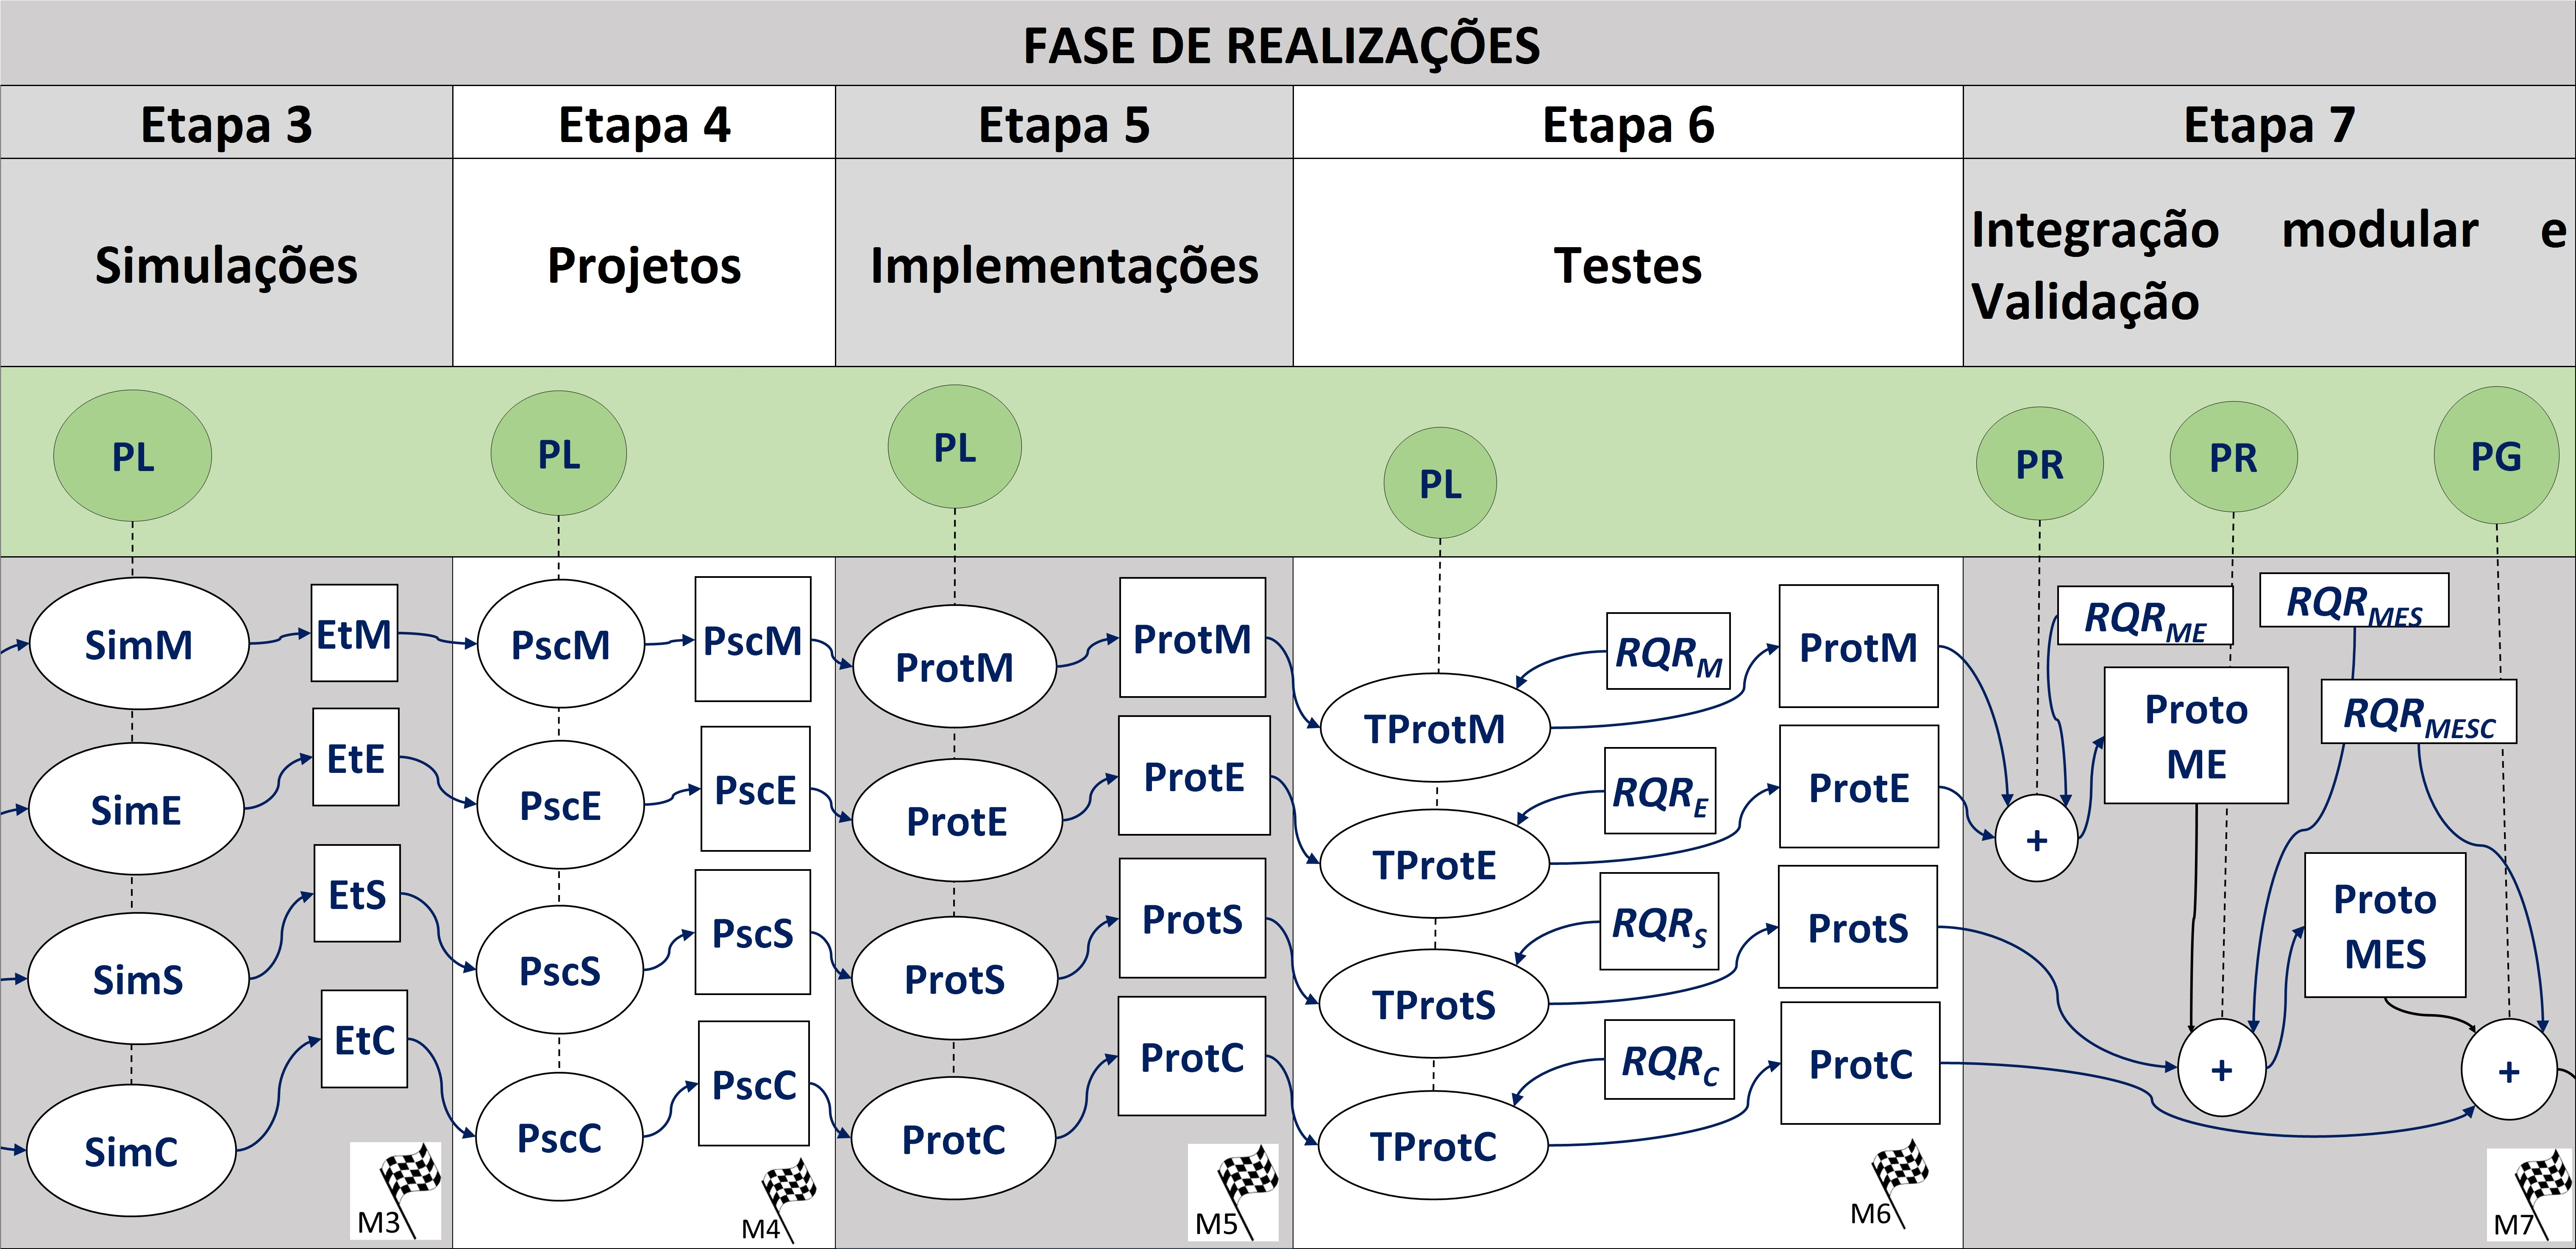
\includegraphics[width=16cm, height=7cm]{F25_SIAPE_VISAO8_1REAL.jpg} 
	\caption{MeDSE - Fase de Realizações}
	\label{F13_2}
\end{figure}
 	
\begin{description}
 	
  \item[Etapa 3 - Simulações] - Na Etapa 3 os requisitos refinados do sistema em forma de problema global (RQRs), na forma regional  (RQRr) e local (RQRl) são modelados e simulados (SimM, SimE, SimS e SimC) até que estes possam ser garantidos para serem confirmados como Especificações Técnicas (Et) de cada problema local, a saber: Especificação Técnica Mecânica (EtM), Especificação Técnica Elétrica (EtE), Especificação Técnica de Software (EtS) e Especificação Técnica de Comunicação (EtC). 
  
  
  \item[Etapa 4 - Projetos] - Na Etapa 4 as especificações técnicas são realinhadas na forma de projetos parciais para formarem o Projeto de Sistema e de Classes de cada problema local (PscM, PscE, PscS e PscC). Nesta etapa cada problema local tem suas especificações refinadas e incluídas no documento de projeto do sistema e entregue como evidência do quarto marco.  
  
  
  \item[Etapa 5 - Implementações] -  Nesta etapa os projetos de cada problema local são implementados, marcando as realizações iniciais dos protótipos locais: Os protótipos da parte mecânica (ProtM), da parte eletrônica (ProtE), da parte de software (ProtS) e da parte de comunicação (ProtC) tornam-se plantas reais dos projetos locais. 
  
  
  \item[Etapa 6 - Testes] - Nesta fase os protótipos construídos são submetidos aos processos de teste (TProtM, TProtE, TProtS e TProtC) contra os requisitos refinados de cada problema local (RQRm, RQRe, RQRs e RQRc). Após a aprovação são levados à condição de protótipos testados e aprovados para o processo de integração.
  
  \item[Etapa 7 - Integração e validação modular] -  Na Etapa 7 os protótipos testados são submetidos ao processo de integração e validação modular:
  
  \begin{enumerate}
  	
  	\item O protótipo mecânico (ProtM) é integrado ao protótipo eletrônico (ProtE) o qual denomina-se protótipo ME (ProtoME);
  	\item O Protótipo ME é então submetido ao processo de validação modular contra os requisitos refinados da entidade ME (RQRme) que representa a realização da solução para a problema regional (ME);
  	\item O ProtoME é integrado ao protótipo da parte de software (ProtS) e a essa integração denomina-se por MES (ProtoMES);
  	\item O protótipo MES é então submetido ao processo de validação modular contra os requisitos refinados da entidade MES (RQRmes) que representa a realização da solução para o problema regional MES;
  	\item O ProtoMES é então integrado ao protótipo da parte de comunicação (ProtC) e com essa integração chega-se à realização da solução do problema global MESC;
  	
  	O protótipo MESC é, então,  enviado à próxima etapa para ser submetidos aos testes de integração e validação sistêmica. 
  	
  \end{enumerate}
  
  Ao final das cinco etapas da fase de realizações, o módulo mecatrônico é concluído.
  
  Tais etapas devem ser realizadas para cada um dos módulos do sistema, que compõem a solução ao PG.
  
  Em todas as etapas do MeDSE existem realimentações de registros que informam se as atividades realizadas estão sendo cumpridas e se as metas de cada etapa foram alcançadas.  Caso não se atinja o desempenho esperado, a etapa é revista objetivando o alcance das metas e a entrega dos marcos do sistema. A Figura \ref{F29} ilustra as realimentações do sistema.
  
  \begin{figure}[h!]
  	\centering
  	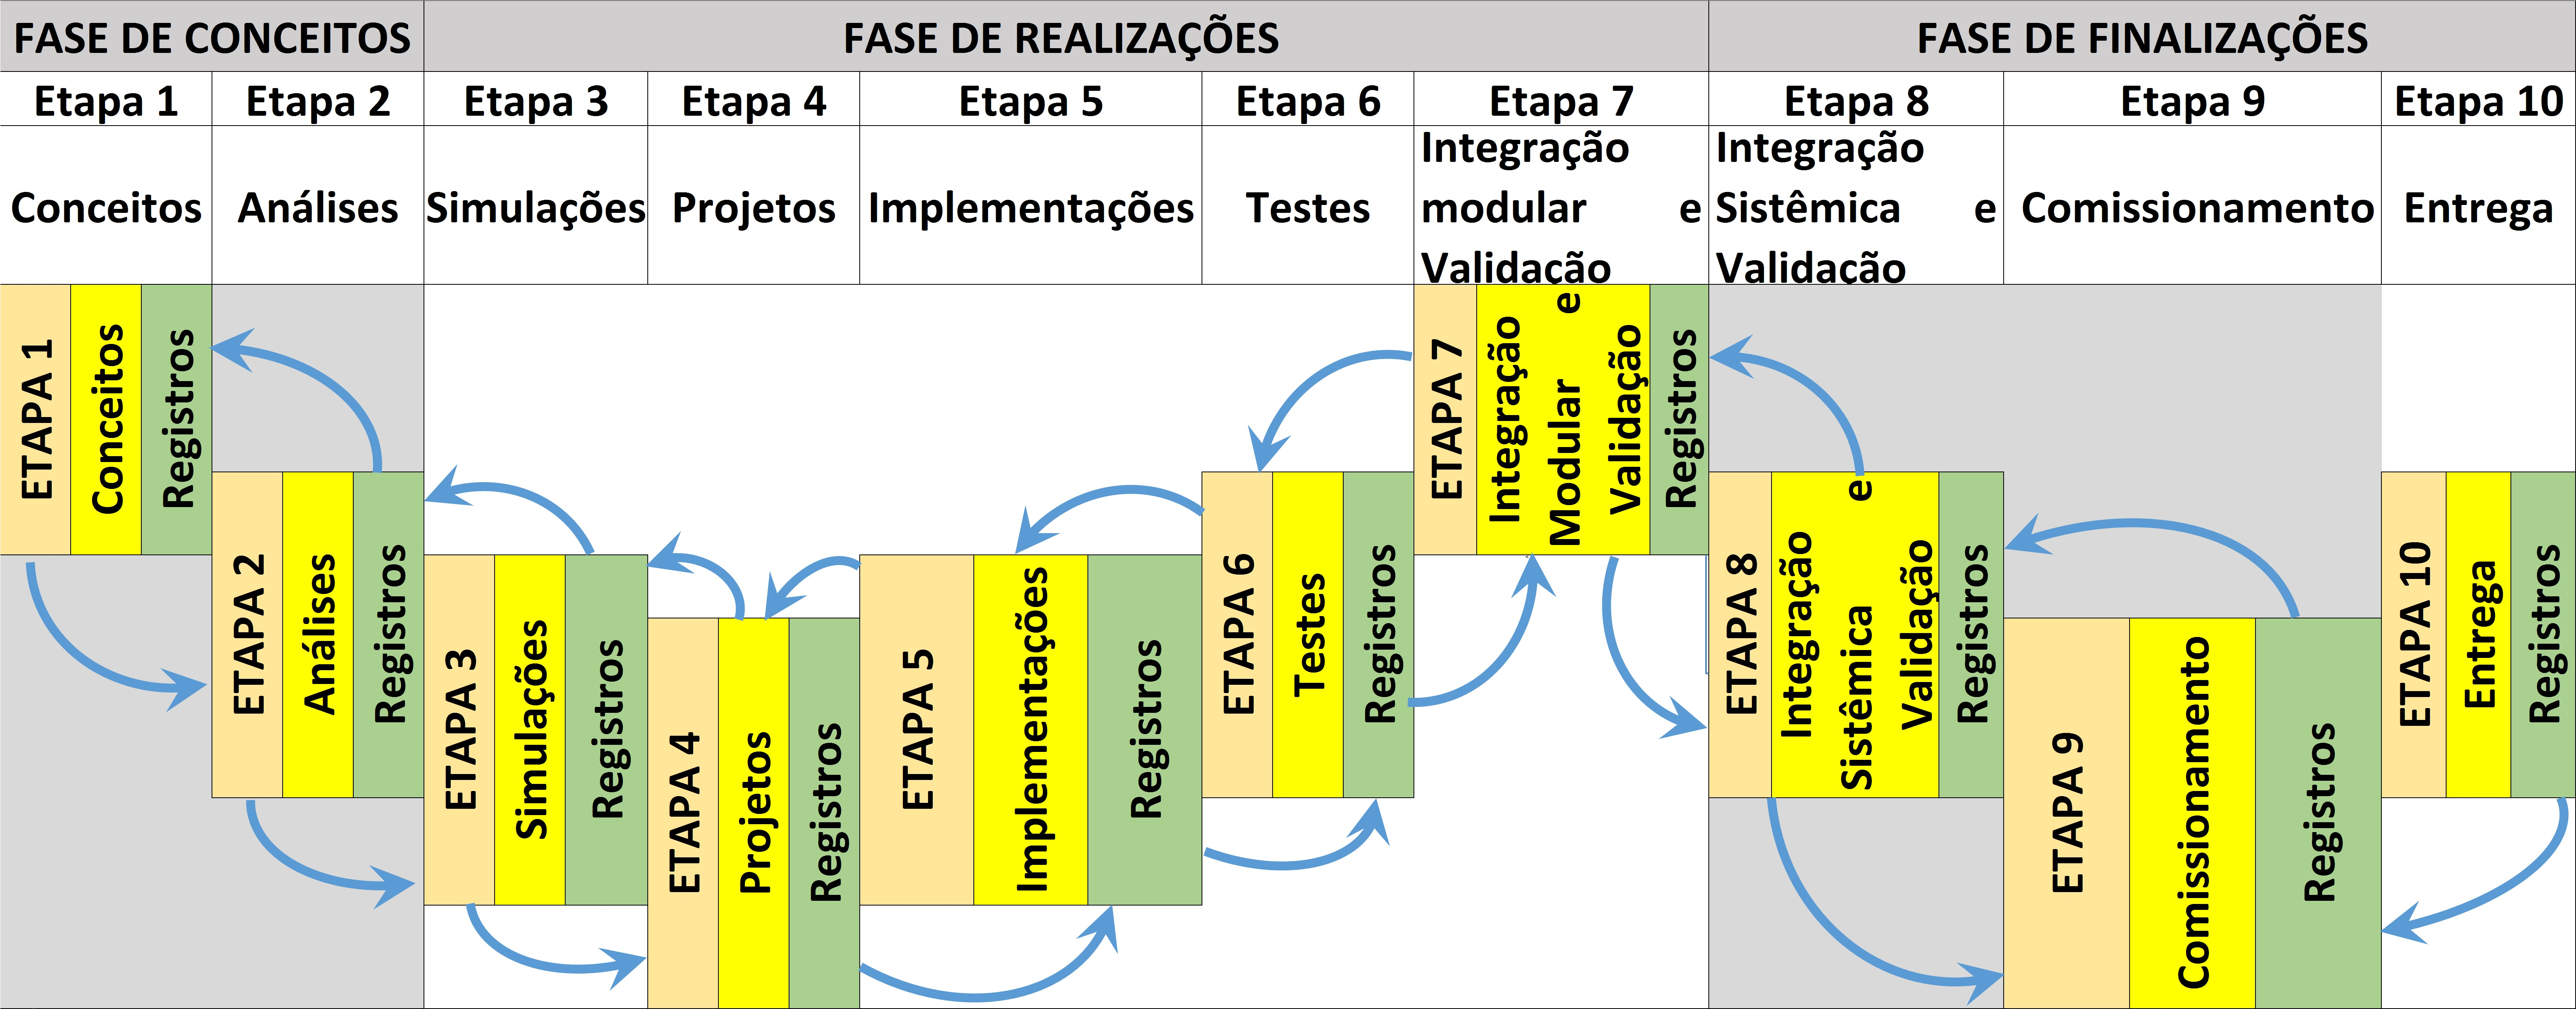
\includegraphics[width=16cm, height=7cm]{F27_SIAPE_REALIMENTACOES1.jpg} 
  	\caption{MeDSE: Realimentações do método}
  	\label{F29}
  \end{figure}
   
\end{description}
 
 
\subsection{A Fase de Finalizações}
 
A Fase de Finalizações tem o principal objetivos de verificar e validar a integração sistêmica do sistema desenvolvido para posterior comissionamento e entrega. A verificação neste trabalho é entendida como a atividade que analisa se os requisitos funcionais e não-funcionais foram atendidos, enquanto a validação analisa se as necessidades do cliente foram atendidas. A verificação e a validação aplicadas nesta fase se justifica devido ao fato do sistema estar totalmente integrado, isto é, antes que o sistema seja entregue ao cliente, a equipe de desenvolvimento deve certificar-se da eficácia das operações do sistema, para  que este, possa então, ser submetido ao comissionamento, etapa na qual os documentos técnicos e de usuário deverão ser validados. De uma forma simplificada, o manual técnico é derivado da verificação e o manual de usuário derivado da validação. Após a realização dessa atividades, o sistema deve estar preparado, por exemplo, a realizar um plano de produção que será solicitado por um usuário do sistema utilizando o manual técnico. Ao se cumprir a meta (a realização do plano)  os agentes mecatrônicos do sistema estarão realizando suas habilidades (skills) evidenciando - juntamente com o restante das atividades desta Fase de Finalizações - que os requisitos do cliente foram atendidos.
  
Essa fase é composta por três etapas ilustrada na Figura \ref{F27_2} e são descritas nas próximas subseções.
 
\begin{figure}
	\centering
	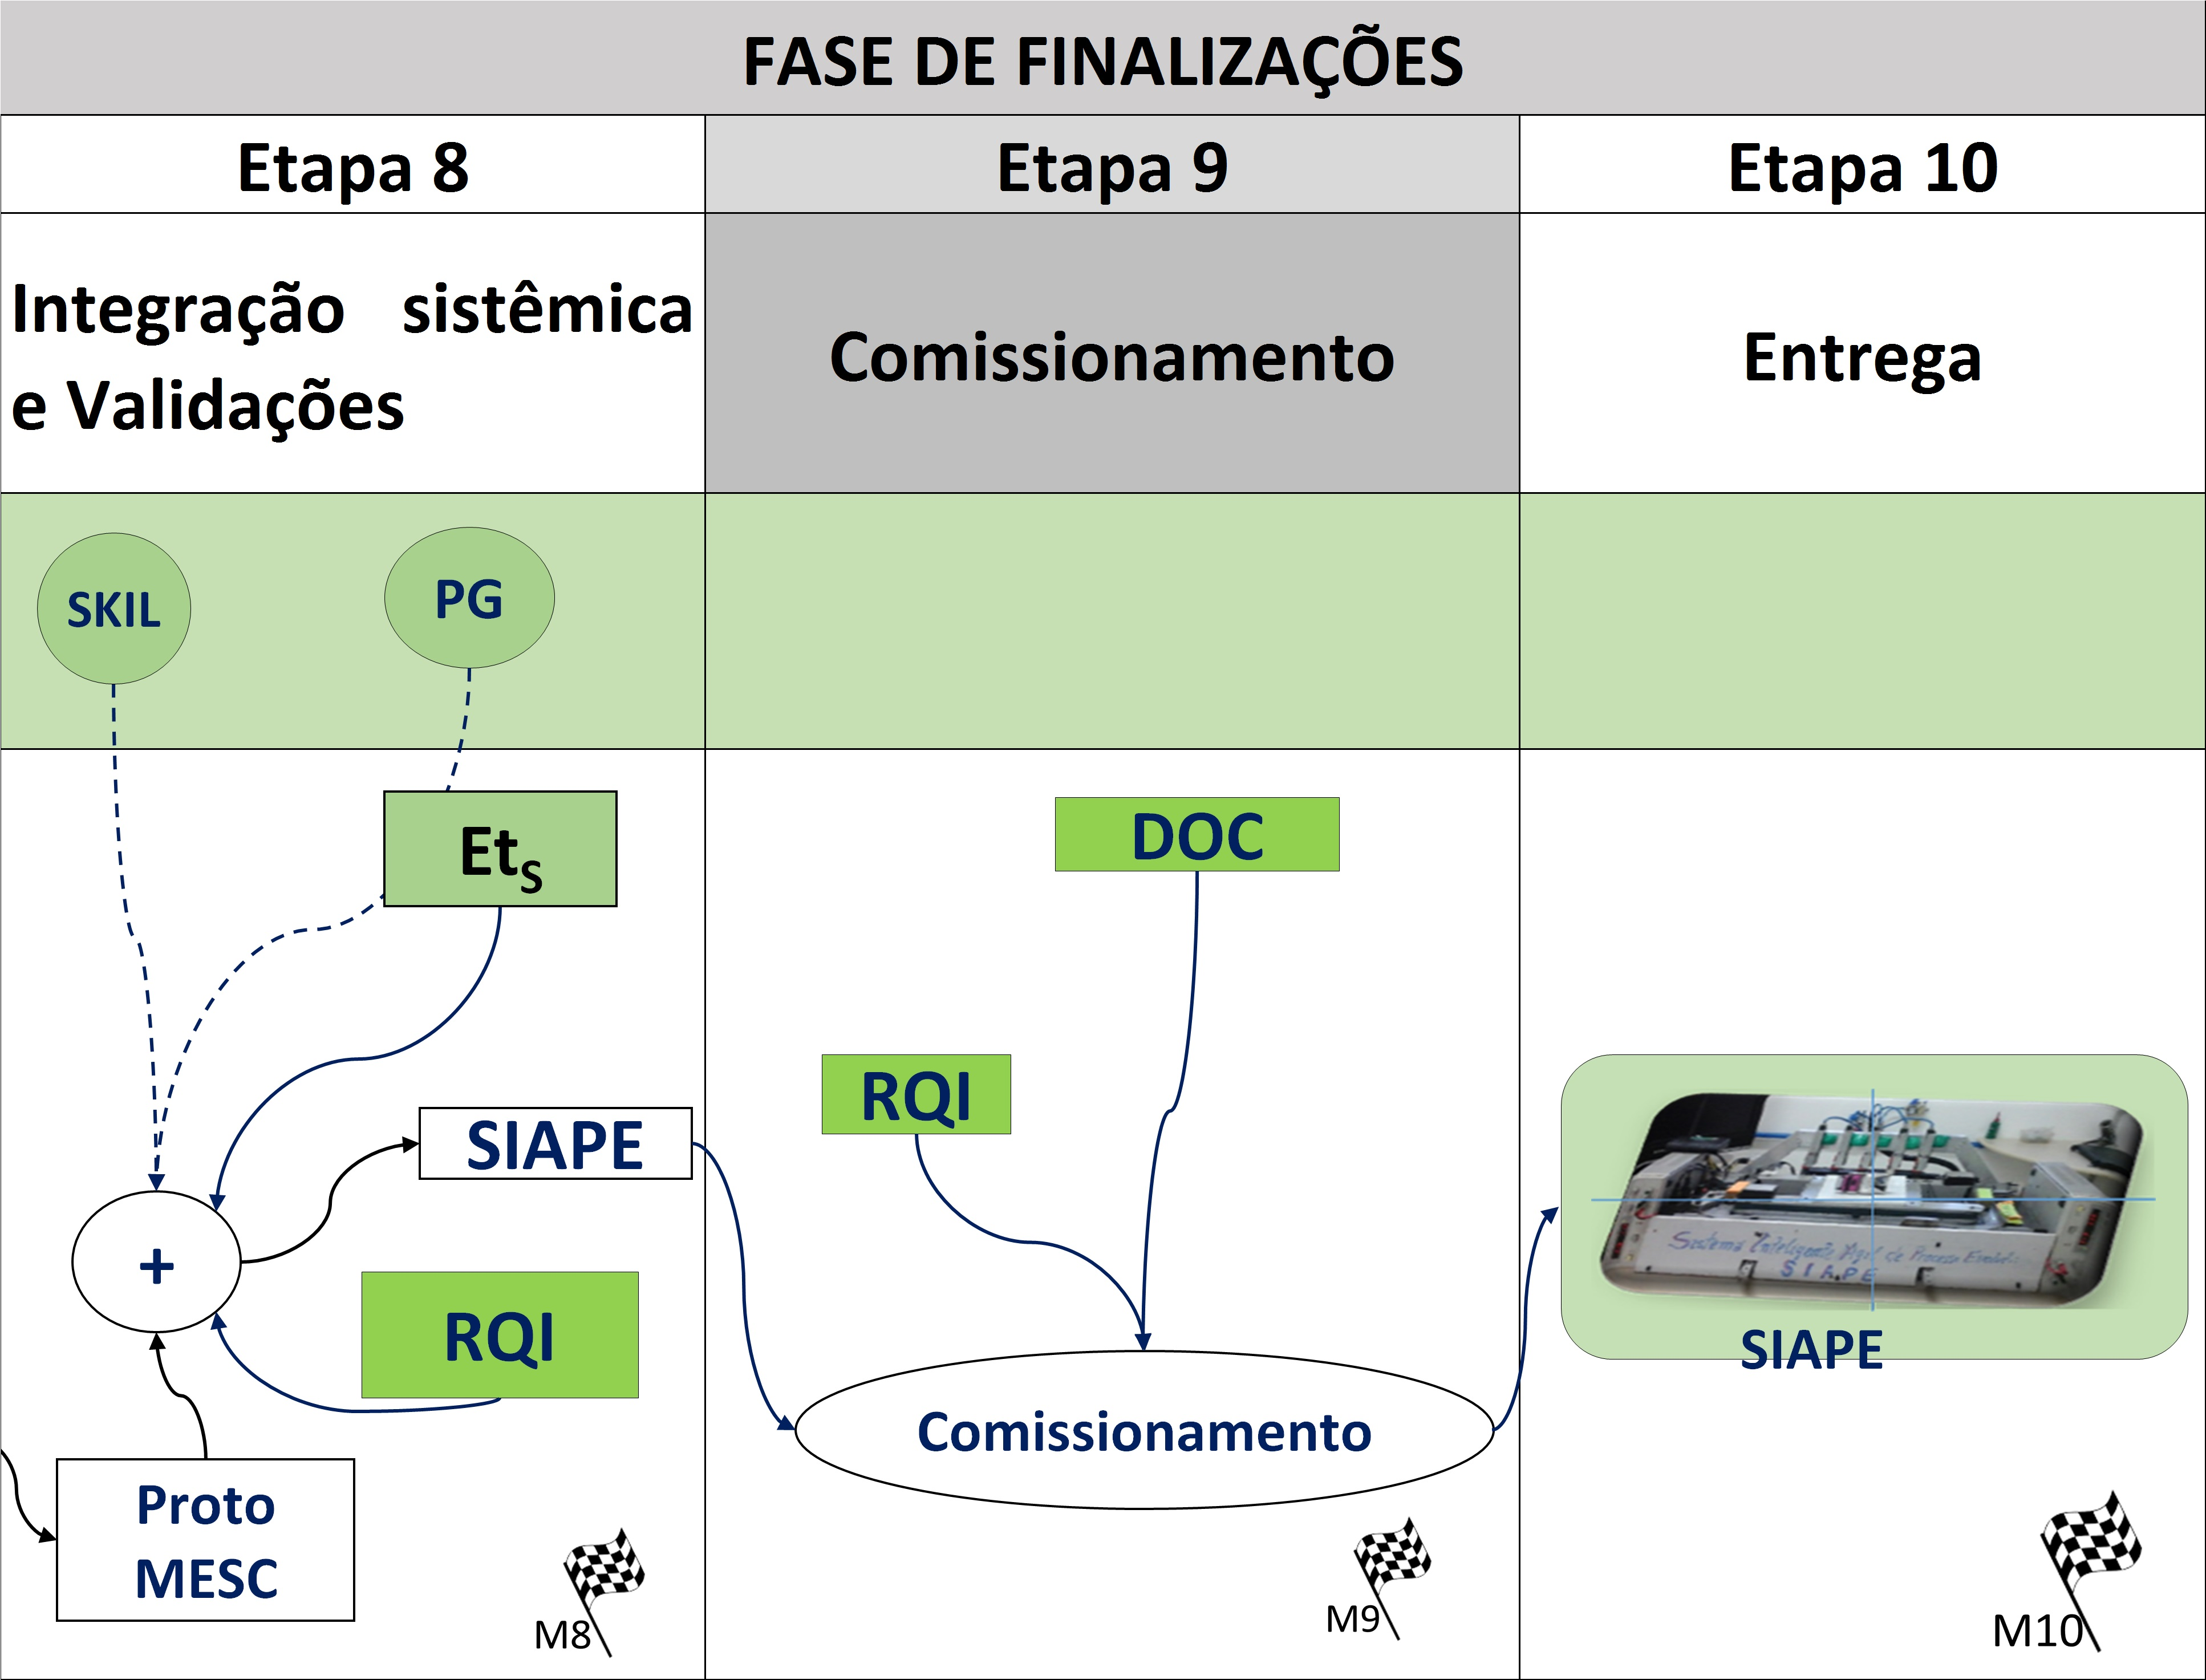
\includegraphics[width=10cm, height=5cm]{F27_2_SIAPE_FINALIZACOES.jpg} 
	\caption{MeDSE: Fase de Finalizações}
	\label{F27_2}
\end{figure}
 
\begin{description}
 	
 	\item[Etapa 8 - Integração e validação sistêmica] - Nesta fase o sistema modular integrado na Etapa 7 é submetido ao processo de integração sistêmica para que seja validado contra os RQI e contra as Ets. Nesta fase o sistema é solicitado a realizar um pedido de usuário que represente uma situação normal de produção. A realização do pedido evidenciará, neste projeto, as atividades dos agentes inteligentes mecatrônicos que se utilizam de seus \textit{skills} para atingir as metas impostas pelo usuário (a realização do pedido). Ao final deste processo têm-se o SIAPE que representa a solução para o problema global identificado pela equipe de desenvolvimento, e que atende aos requisitos do solicitados pelo cliente. 
 	
 	\item[Etapa 9 - Comissionamento] - Na Etapa 9 a documentação técnica, e do usuário, é finalizada e o sistema é comissionado contra o manual de operação técnica, e contra o manual de usuário. É importante notar, que mesmo nesta etapa, os registros que identificam se as metas foram alcançadas utilizam-se dos RQI para elucidar qualquer potencial inconsistência surgida. 
 	
 	\item[Etapa 10 - Entrega] - Na Etapa 10 o sistema é demonstrado ao cliente e entregue oficialmente, encerrando a fase de desenvolvimento. Na comparação ilustrada na Figura \ref{F13_1},  \citeonline{RUMBAUGH2006} propõe, após a implantação, a fase de manutenção do sistema. Como o foco desse trabalho de pesquisa é o de sistemas evolutivos, a fase de manutenção faz parte da evolução e adaptação do sistema e é realizada pela equipe de desenvolvimento de acordo com o tempo definido em contrato para esse fim.  
\end{description}
 	
 	
%================================ APLICAÇÃO DO MEDSE AO SIAPE =================================
\cleardoublepage
\section{Aplicação do MeDSE ao SIAPE}

Esta seção descreve a aplicação do MeDSE na realização do SIAPE, por meio das descrições dos procedimentos práticos realizados no desenvolvimento de cada etapa do método. Para que a descrição reflita os passos e facilite entendimento dos mesmos,  cinco itens foram definidos e encontram-se ilustrados na Tabela~\ref{T2}. 

%===============================

\begin{table}[htb]
	\center
	\footnotesize
	\begin{tabular}{|p{1.4cm}|p{1cm}|p{3cm}|p{3cm}|}
		\hline
		\textbf{Folha} & \textbf{Linha}  & \textbf{Onde se lê}  & \textbf{Leia-se}  \\
		\hline
		1 & 10 & auto-conclavo & autoconclavo\\
		\hline
	\end{tabular}
\end{table}
%----------------------------------

\begin{table}[h]
	\centering
	\caption{Itens processados em cada etapa}
	\begin{tabular}{|l| p{13.5cm}| c| c| } \hline
		\textbf{ Item} 	   & \textbf {Descrição}	 \\ \hline
		\textbf{1.Objetivos}   & Descrição do objetivo da etapa \\ \hline
		\textbf{2.Entradas}	   & Identificação das entradas no processo de transformação da etapa  \\ \hline
		\textbf{3.Processo }    & Processo que transforma as entradas em saídas \\ \hline
		\textbf{4.Saídas}		  & Resultado da realização do processo de transformação. Igual ao marco da etapa\\ \hline
		\textbf{5.Registros}	 & Documentos gerados na etapa e, se necessário geram realimentações \\ \hline
	\end{tabular}
	\label{T2}
	%	Fonte: Hiram Amaral
\end{table}

Essa tabela é utilizada no procedimento padrão adotado para descrever as etapas, e este foi seguido durante todo o desenvolvimento do SIAPE. A Figura \ref{F50} ilustra o procedimento que é dividido em duas parte e sua explicação é feita a seguir:

\begin{description}
	\item[Primeira parte] - Em todas as etapas os cinco itens definidos  são descritos numa tabela;
	\item[Segunda parte] - A etapa é descrita textualmente, e onde aplicável, figuras são ilustradas. 
\end{description}


 \begin{figure}[h]
 	\centering
 	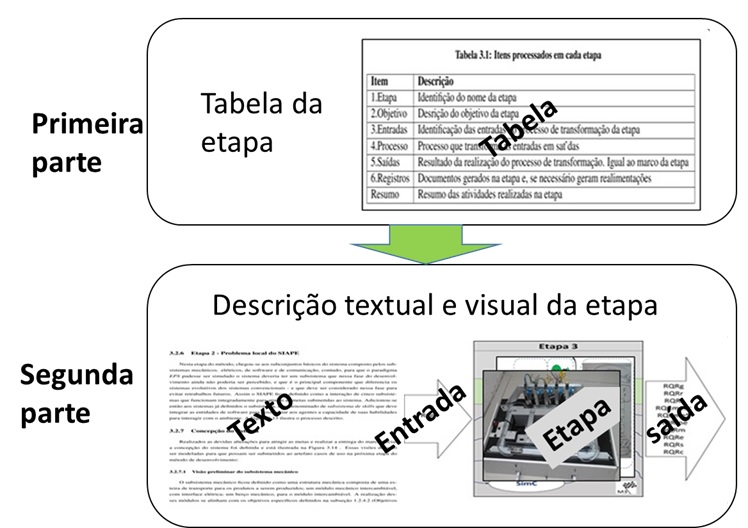
\includegraphics[width=8cm, height=5cm]{F50_MEDSE_2FORMAS1.jpg} 
 	\caption{MeDSE: Descrição da atividades nas etapas}
 	\label{F50}
 \end{figure}


 A descrição textual e visual da etapa expande, resumidamente, os títulos relacionados na tabela. A visualização evidencia pontos relevantes através de fotos, diagramas, esquemas ou figuras. \par 

%=================================================

Realizadas as explanações sobre o MeDSE e definido o procedimento padrão, espera-se que o projetista esteja habilitado para seguir a aplicação do  MeDSE e realizar o SIAPE.
\cleardoublepage
%++++++++++++++++++++++++++++++++++++++++++++++++++++++++++++++++++++++++++++++++++++++++++++++++++++++++++++++
\subsection{ETAPA 1 - CONCEITOS}

\begin{description}

\begin{table}[htbp]
	\centering
	\caption{Tabela da etapa 1 - Conceitos}
	%=================================================================================================
	\begin{tabular}{|l| p{13.5cm}| c| c| } \hline
		%================================================================================================
		\textbf {Item} 	   & \textbf {Descrição}	 \\ \hline
		%================================================================================================
		\textbf{1. Objetivos} &  
		Elaborar a concepção do sistema\\ \hline
		%================================================================================================
		\textbf{2. Entradas}  &		 
		1 -- As necessidades do cliente\par  	
		2 -- Referenciais específicos do Paradigma EPS\par 	
		3 -- Referenciais externos relacionados ao sistema  \\ \hline	
		%================================================================================================	
		\textbf{3. Processo}    & Gerar requisitos \\ \hline
		%================================================================================================
		\textbf{4. Saídas}	     & 
		Documento de Concepção do sistema contendo os requisitos iniciais (RQI) e o problema global (PG)\\ \hline
		%================================================================================================		
		\textbf{5. Registros}	& 	
		1 --Documento de Concepção do sistema \par
		2 -- Diagrama de Requisitos Pai \par
		3 -- Diagrama de Requisitos filhos\\ \hline
		%================================================================================================
	\end{tabular}
	\label{T3}\par
	%	Fonte: Hiram Amaral
\end{table}

\item[Descrição textual e visual da etapa] - Os conceitos, requisitos e restrições foram esquematizados para que o Problema Global fosse elaborado, A Figura \ref{F62} ilustra a sintetização que gerou o Problema Global (PG).  O PG também pode ser representado pelas partes do sistema M, E, S, C e SK (Skills).


\end{description}

\begin{figure}[!h]
	\centering
	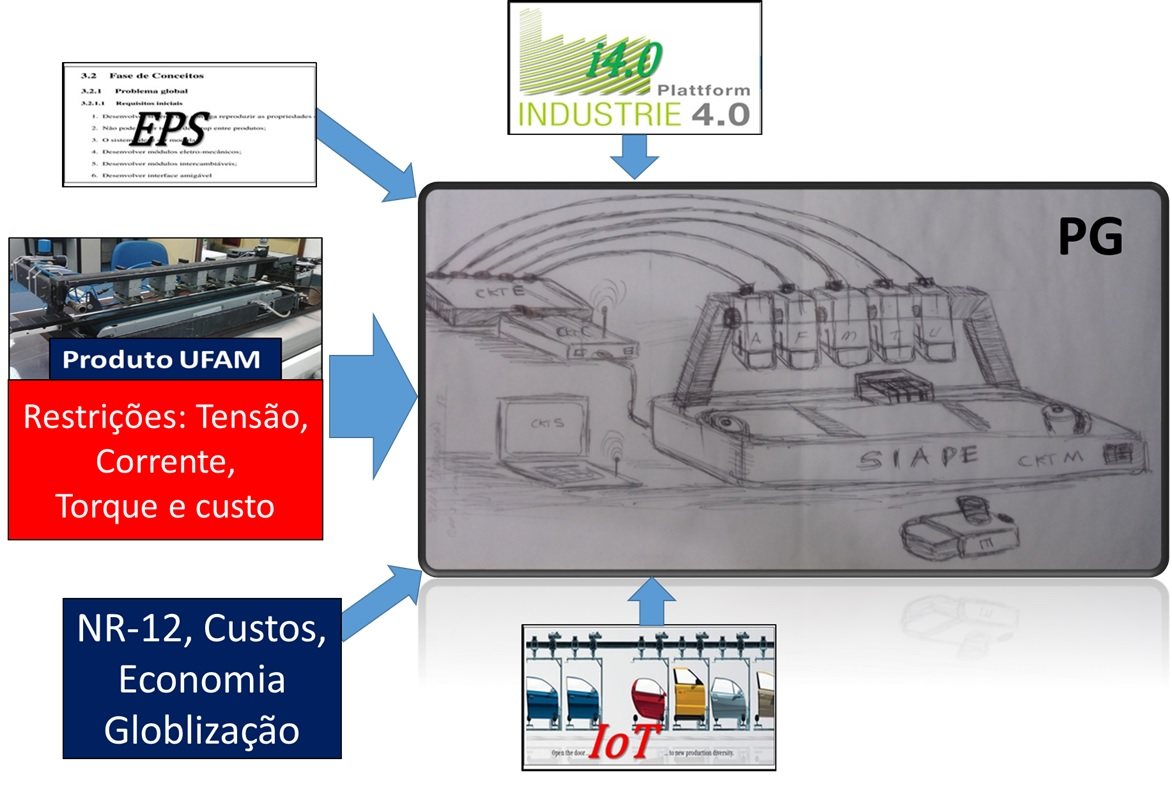
\includegraphics[width=14cm, height=8cm]{F62_SIAPE_PG.jpg} 
	\caption{SIAPE: Problema Global}
	\label{F62}
\end{figure}
Para desenvolver a concepção do sistema, as necessidades do cliente são consideradas, a saber:\par   	
a.	Desenvolver um sistema que consiga expressar as características dos sistemas evolutivos e evidenciar potenciais capacidades para reduzir o problema da customização de massa. Além disso, o sistema deve considerar alguma recomendações da Plataforma da Indústria 4.0 (i4.0) e capturar algum conceito da arquitetura Internet das Coisas (IoT) no tocante Manufatura Ágil. \par 
b.	O sistema deve ser baseado no Produto UFAM com as devidas alterações de melhorias; \par 
c.	O sistema deve carimbar as 5 letras A, F, M, T  e U; \par 
d.	Deverá ser criado um módulo para letra que seja exigido em nova palavra; \par 
e.	O sistema de carimbar as palavras UFAM, UTAM e UEA; \par 
f. O sistema deveria ser baseado no Produto UFAM.\par
Somam-se às necessidades do cliente, os referenciais específicos do Paradigma \textit{EPS}. Das características básicas do Paradigma \textit{EPS} extraiu-se capacidade de \textit{adaptação}, implicando que o sistema deve ser capaz de propor uma alternativa de configuração para minimizar os efeitos de perturbarções externas, e a capacidade de \textit{evolução}, implicando que o sistema deve ser capaz de aceitar a troca de módulos em tempo de produção. \par 

Para realizar as principais características as propriedades da Modularidade, Granularidade, Plugabilidade e Reconfigurabilidade devem estar presente no sistema.\par 
%\textbf{Modularidade}: a noção de módulos independentes devem estar presente no sistema EPS. \par  
\ %textbf{Plugabilidade:} A capacidade de lidar com a introdução de novos módulos, enquanto o sistema está funcionando. O sistema deve ser capaz de redesenhar a dinâmica %interna, a fim de manter a sua eficiência. \par  
%\textbf{Reconfigurabilidade:} O sistema precisa ser capaz de lidar com o redesenho do layout sem comprometer qualquer funcionalidade.
	
Além dos referenciais do cliente e de EPS são considerados os referenciais externos relacionados ao sistema:	 \par 
\textbf{Academia} - O sistema deve refletir o estado da arte em paradigmas de manufatura.\par 
\textbf{Globalização} -  O sistema deve evidenciar potenciais soluções para a questão da customização de massas.\par 
\textbf{Indústria 4.0} - A integração horizontal definida como a agregação, em tempo real dos elementos de sistemas no chão--de--fábrica, relacionando a comunicação, o planejamento e a programação desses sistemas, contendo elementos que serão usados para incorporar raciocínio baseado em casos de uso, evidenciando a capacidade de evoluir com a mudança dos requisitos de produção, deverá estar presente no sistema.\par 
\textbf{Internet das Coisas} -  O conceito plugar e trabalhar \textit{ Plug \& Work}  é definido como a capacidade de dispositivos e componentes de rede para auto-configurar-se de acordo com as necessidades das aplicações da automação. \textit{Plug \& Work} deve trabalhar em ambientes 4.0 e reduzir maciçamente as ações manuais e reduzirá tanto o tempo de inatividade global quanto o número de erros do sistema.\par 
\textbf{Governo} -  Para atender a exigência de segurança, o governo editou a Norma Regulatória número 12 (NR-12) que de acordo com o item 12.56, as máquinas devem ser equipadas com um ou mais dispositivos de parada de emergência, por meio dos quais possam ser evitadas situações de perigo latentes e existentes.\par 
\textbf{Economia} -  Por meio da redução de custos no processo produtivo incrementa-se o nível de competitividade dos produtos originados nesse processo. Portanto, as vantagens comparativas entre o SIAPE e os sistemas de produção vigentes tendem a se transformar em ganhos de competitividade, e deverão ser mensurados e quantificados no processo evolutivo. \par 
As necessidades do cliente, os referenciais internos e os referenciais externos foram sintetizados na geração dos RQI conforme ilustra a Figura \ref{F61}. 

\begin{landscape}
	\begin{figure}[!h]
		\centering
		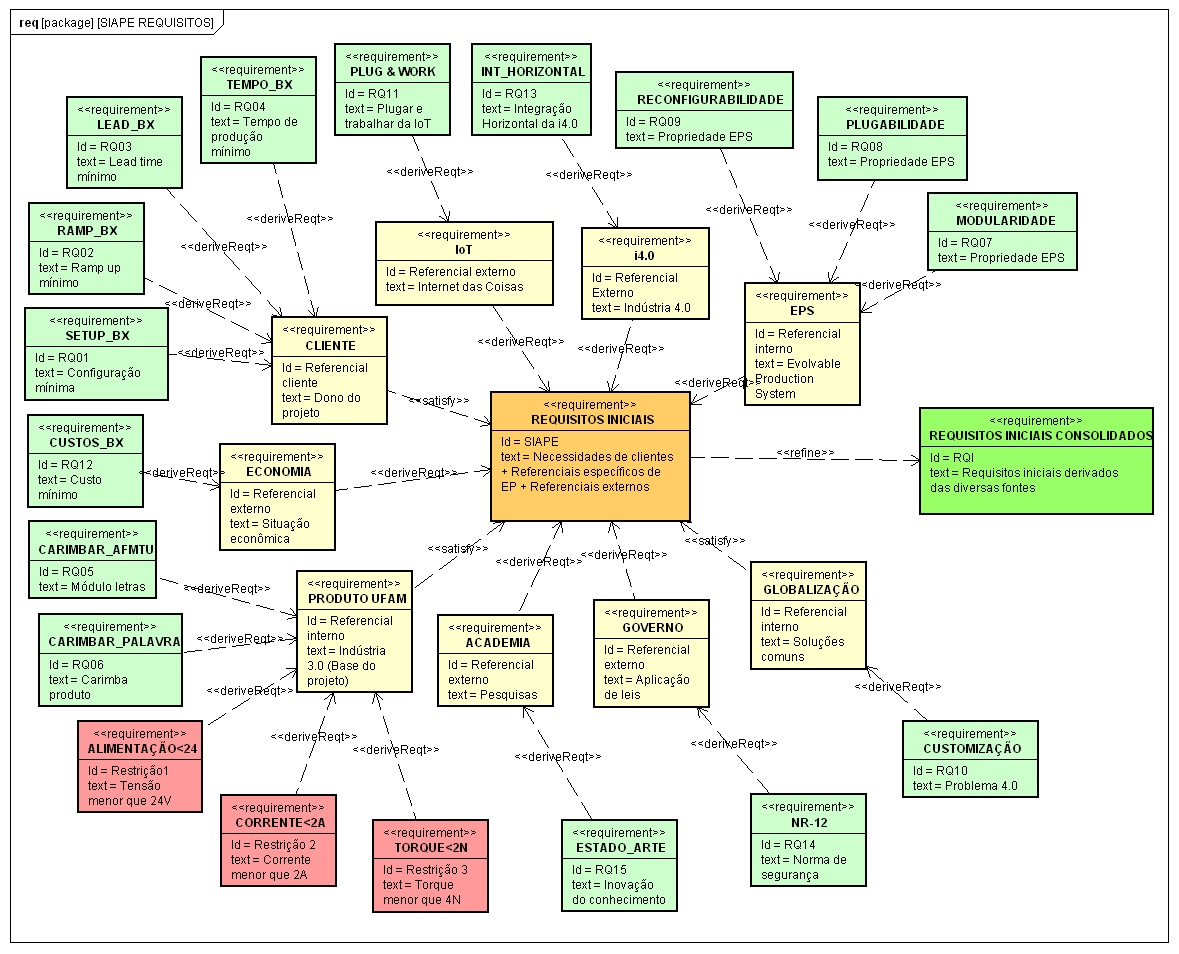
\includegraphics[width=24cm, height=14cm]{F61_SIAPE_REQUISITOS_V03.jpg} 
		\caption{SIAPE: Requisitos}
		\label{F61}
	\end{figure}
\end{landscape}


A Figura \ref{F61} ilustra  o processo de agregação dos requisitos do sistema em tipos de requisitos. Tais agregações são filtradas produzindo em sua saída uma relação de requisitos, denominados de requisitos iniciais que serão submetidos ao processamento da próxima etapa. 

Na saída do processo têm-se o Documento de Concepção do sistema contendo os requisitos iniciais (RQI) e o problema global (PG).

A ilustração da Figura \ref{F64}  detalha a visão da concepção do sistema. Nesta figura está montado o cenário para as verificações e validações finais realizadas na Fase de Finalizações do método de desenvolvimento. Quando um pedido é realizado por clientes, estes pedidos são inseridos por um operador na Interface Homem Máquina (IHM). A partir da inserção dos pedidos na IHM, o agente Order solicita ao agente YPA os nomes dos módulos que estão presentes no sistema. Com a informação fornecida o agente Order cria o plano de produção e envia ao agente Anagrama. O Anagrama realiza o plano enviando os comandos ao agente AcHw (Acesso Hardware). O AcHw envia os comando através do \textit {Raspberry Pi} à parte elétrica, que ativa os atuadores e realiza os produtos solicitados pelos clientes. O operador entrega os produtos a seus respectivos clientes e o ciclo se fecha.     

\begin{figure}[!h]
	\centering
	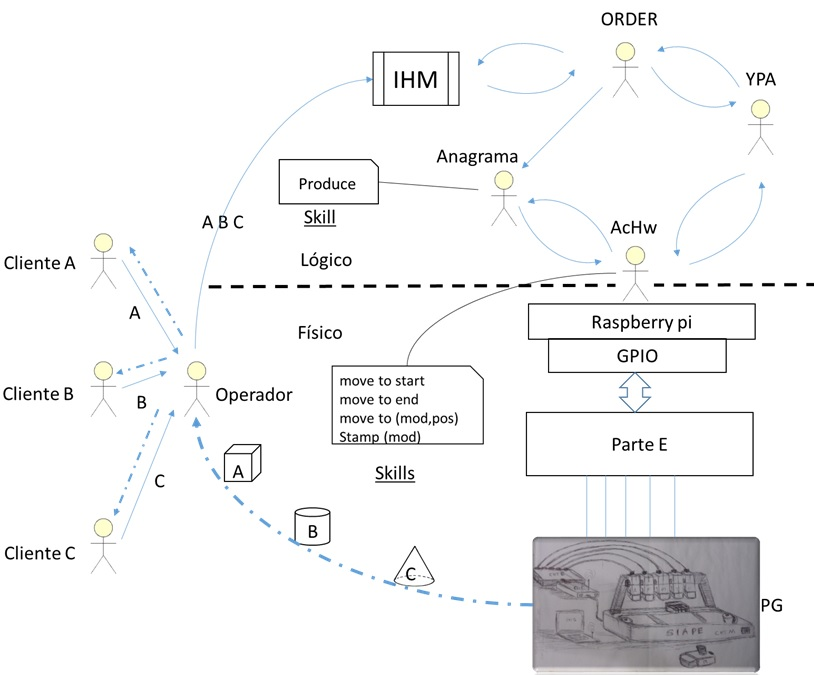
\includegraphics[width=16cm, height=10cm]{F64_SIAPE_VISAO_CONCEPCAO_SISTEMA.jpg} 
	\caption{SIAPE: Cenário concepção do sistema}
	\label{F64}
\end{figure}


O entendimento das funções de parte do sistema é fundamental para a realização da Etapa~2. Para compatibilizar  alguns parâmetros entre Produto UFAM e SIAPE foi assumido como restrição que a alimentação máxima do sistema deveria ser <~24V, com uma corrente <~2A e um custo máxima da ordem de dez vezes o valor investido no Produto UFAM. 

Os RQI e o PG originaram o documento de Concepção do Sistema que contém as informações de entrada para a próxima etapa. A Figura \ref{F63} ilustra a inclusão do RQI e PG no documento de Concepção do Sistema SIAPE e evidencia a realização do segundo marco: Entrega do Documento de Concepção do Sistema.

\begin{figure}[!h]
	\centering
	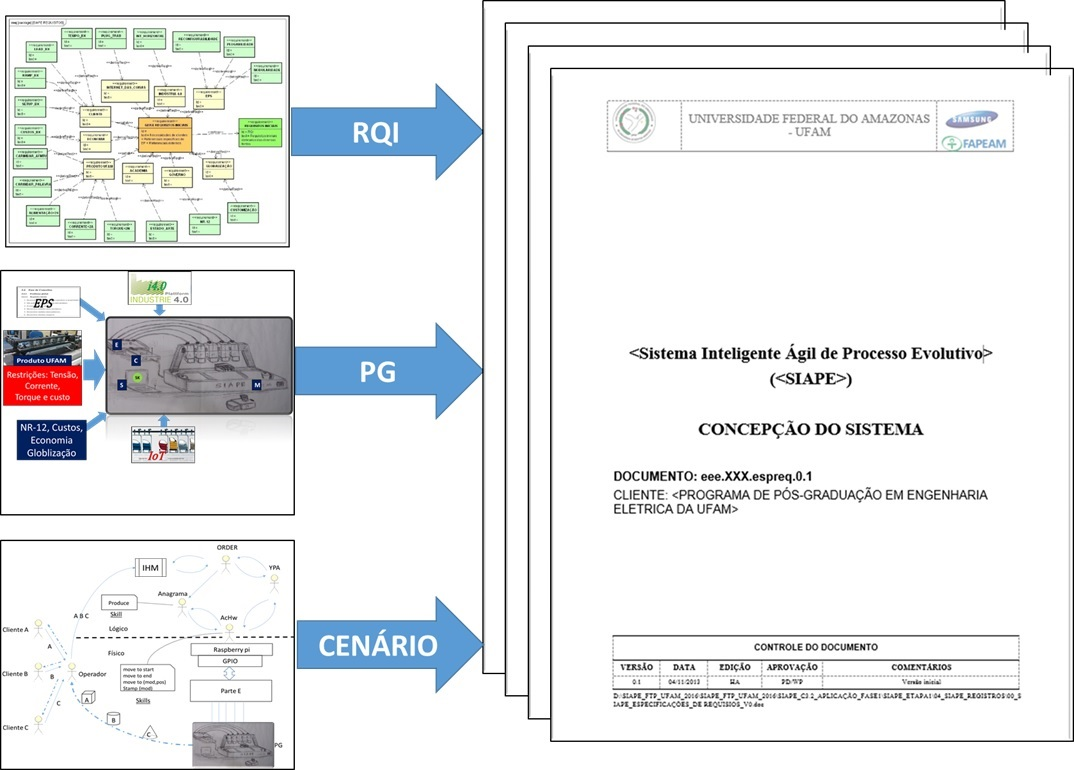
\includegraphics[width=16cm, height=10cm]{F63_SIAPE_CONCEPCAO_SISTEMA.jpg} 
	\caption{SIAPE: Geração do documento de concepção do sistema}
	\label{F63}
\end{figure}

Ao entregar o Documento de Concepção do Sistema contendo os Requisitos Iniciais (RQI), a definição do Problema Global (PG) e o Cenário que deverá ser utilizado para validar o sistema (na Fase de Finalizações), o objetivo da etapa é atingido.


\cleardoublepage
  %+++++++++++++++++++++++++++++++++++++++++++++++++++++++
\subsection{ETAPA 2 - ANÁLISES}
\begin{description}
\begin{table}[htbp]
	\centering
	\caption{Tabela da etapa 2 - Análises}
	%=================================================================================================
	\begin{tabular}{|l| p{13.5cm}| c| c| } \hline
		%================================================================================================
		\textbf{Item} 	    & \textbf{Descrição} 
		\\ \hline
		%================================================================================================
		\textbf{1.Objetivo}	   &  
		Refinar os requisitos inciais do cliente (RQI)\\ \hline
		%================================================================================================
		\textbf{2.Entradas}	  &		
		Documento de Concepção do sistema contendo os requisitos iniciais (RQI) e o problema global (PG)\par  	
		\\ \hline	
		%================================================================================================	
		\textbf{3.Processo}     &
		Refinar RQI\\ \hline
		%================================================================================================
		\textbf{4.Saídas}		& 
		Requisitos refinados (RQR): RQRmesc, RQRmes, RQRme, RQRm, RQRe, RQRs, RQRc, RQRa, RQRf, RQRm, RQRt RQRu 
		\\ \hline
		%================================================================================================		
		\textbf{5.Registros}   & 	
		Planilha de requisitos refinados do sistema\\ \hline
		%================================================================================================
	\end{tabular}
	\label{T4}\par
	%	Fonte: Hiram Amaral
\end{table}

\item[Descrição textual e visual da etapa] - A Etapa de Análises tem o objetivo de refinar os requisitos inicias e especificá-los para cada parte do Problema Global em sua forma MESC. \par 
Os requisitos iniciais (RQI) e o problema global (PG) contidos no Documento de Concepção do Sistema são divididos para serem refinados. 	O Problema Global (PG) é convenientemente dividido em Problema Regional (PR) e Problema Local (PL) e são relacionados com as partes do sistema mecatrônico MESC: MESCmain, MES, ME, M, E, S, C, MESCA, MESCF, MESCM, MESCT e MESCU e MESCE. Onde:

\item[Definição dos agentes baseada na Arquitetura SIAPE] - Para a definição da quantidade e do tipo de agentes a serem utilizados na proposta de solução ao PG foram definidos os seguintes agentes da arquitetura aserem implementados:

\begin{description}
	\item[01 YPA ]- Para registrar os agentes existentes na plataforma e buscar seus \textit{skills}.	
	\item[01 OrderAgent] - Com a função de\textit{GATEWAY} para a interface homem máquina do EPS e instanciar os anagramas de acordo com a ordem de serviço gerada na IHM.	
	\item[01 Anagram] - Para representar os produtos (ANAGRAMA) a serem produzidos.
	\item[01 AcHw] - Para detectar e informar os módulos disponíveis no sistema.
	\item[01 Conveyor] - Para representar a ESTEIRA do sistema que realizar o transporte dos produtos.	
	\item[01 Stamper] - Para representar os MÓDULOS CARIMBADORES do sistema e carimbar as letras do anagrama na palete.
\end{description}
\end{description}

	A Figura \ref{F145} mostra os agentes da arquitetura SIAPE aplicados ao caso do PG. Essa aplicação, neste momento do desenvolvimento, torna-se necessária para evidenciar um exemplo prático da arquitetura que foi implementado neste etapa, e experimentado e validado nos Capítulos 4 e 5.
	
	\begin{figure}[h]
		\centering
		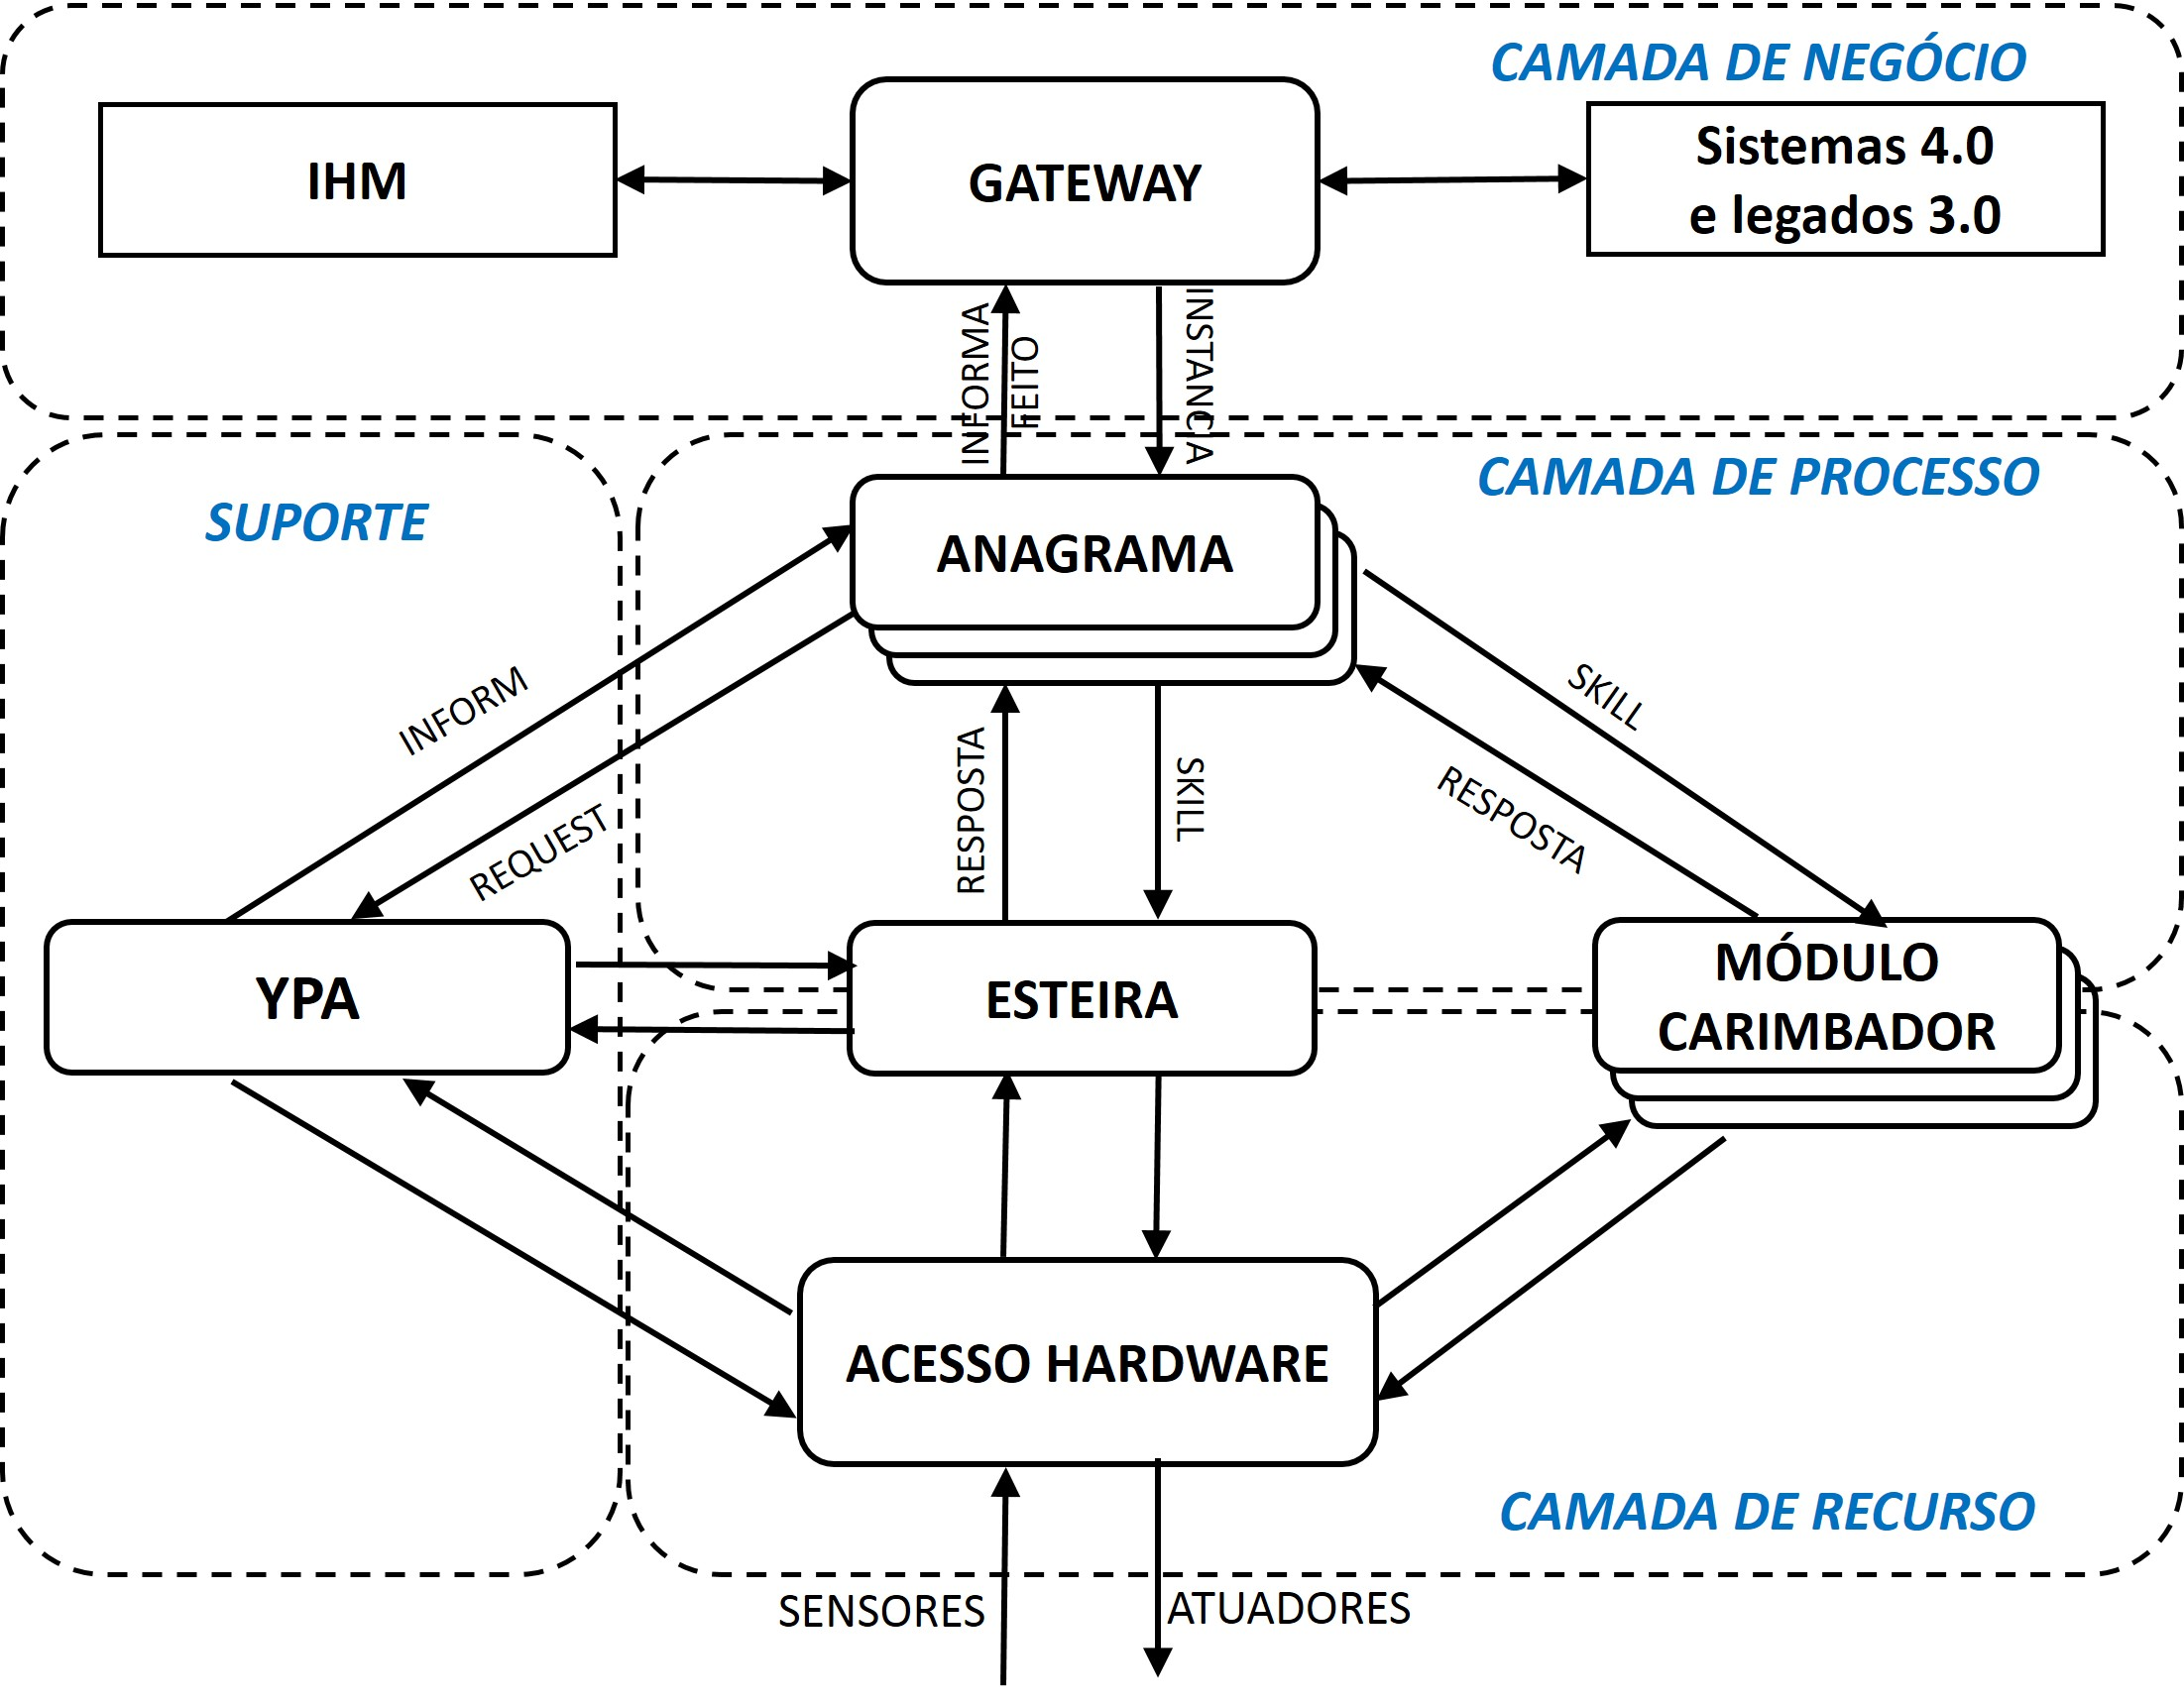
\includegraphics[width=12cm, height=9cm]{F144_arquitetura_PG.jpg} 
		\caption{SIAPE: Arquitetura SIAPE aplicada ao PG}
		\label{F145}
	\end{figure}

	\begin{description}
			\item[MESCmain] - representa a parte do MESC principal  do sistema contendo a integração das partes M, E, S e C e tem seus requisitos refinados e rotulados como RQRmesc;
			\item[MES] - representa a parte do MESC contendo a integração das partes M, E e S do MESC principal e tem seus requisitos refinados o rotulados como RQRmes;
			\item[ME] - representa a parte ME do MESC contendo a integração das partes M e E e tem seus requisitos refinados e rotulados como RQRme;
			\item[M] - representa a parte mecânica do MESC principal e tem seus requisitos refinados e rotulados como RQRm;
			\item[E] - representa a parte eletrônica do MESC principal e tem seus requisitos refinados e rotulados como RQRe;
			\item[S] - representa a parte de software do MESC principal e tem seus requisitos refinados e rotulados como RQRs;
			\item[C] - representa a parte comunicação do MESC principal e tem seus requisitos refinados e rotulados como RQRc;
			\item[MESCa] - representa o módulo mecatrônico que realiza a letra A e  tem seus requisitos rotulados como RQRA;
			\item[MESCf] - representa o módulo mecatrônico que realiza a letra F e  tem seus requisitos rotulados como RQRF ;
			\item[MESCm] - representa o módulo mecatrônico que realiza a letra M e  tem seus requisitos rotulados como RQRM; 
			\item[MESCt] - representa o módulo mecatrônico que realiza a letra T e  tem seus requisitos rotulados como RQRT;
			\item[MESCu] - representa o módulo mecatrônico que realiza a letra U e  tem seus requisitos rotulados como RQRU;
			\item[MESCe] - representa o módulo mecatrônico que realiza a letra E e  tem seus requisitos rotulados como RQRE.		
	\end{description}
	
O resultado na  saída do processo é o conjunto de documentos relacionados a seguir e que servem como registros das atividades realizadas. 	

		\begin{description}
			\item[MESCmain] - Documento de requisitos refinados do MESC principal;
			\item [RQRmes] - Documento de requisitos refinados das integrações MES e ME;
			\item[RQRm] - Documento de requisitos refinados da parte atômicas M, E, S e C do MESC principal;
			\item[RQRA] - Documento de requisitos refinados dos módulos mecatrônicos A, F, M, T, U e E;
		\end{description}

A Fase de Conceitos que realiza a Concepção do Sistema define uma ideia de sistema baseado na solicitação do cliente,  nas exigências internas, nas exigências externas e nas restrições. O segundo marco registra essa ideia por meio da entrega dos Requisitos Refinados. O conteúdo produzido até este momento deve ser confirmado, para que possa ser garantido como especificação e assumido como um projeto a ser realizado.  A Figura \ref{F65} ilustra os módulos de hardware e software que foram definidos para serem simulados ou verificados para que possam ser confirmados como especificações técnicas. \par 

\begin{figure}[h]
	\centering
	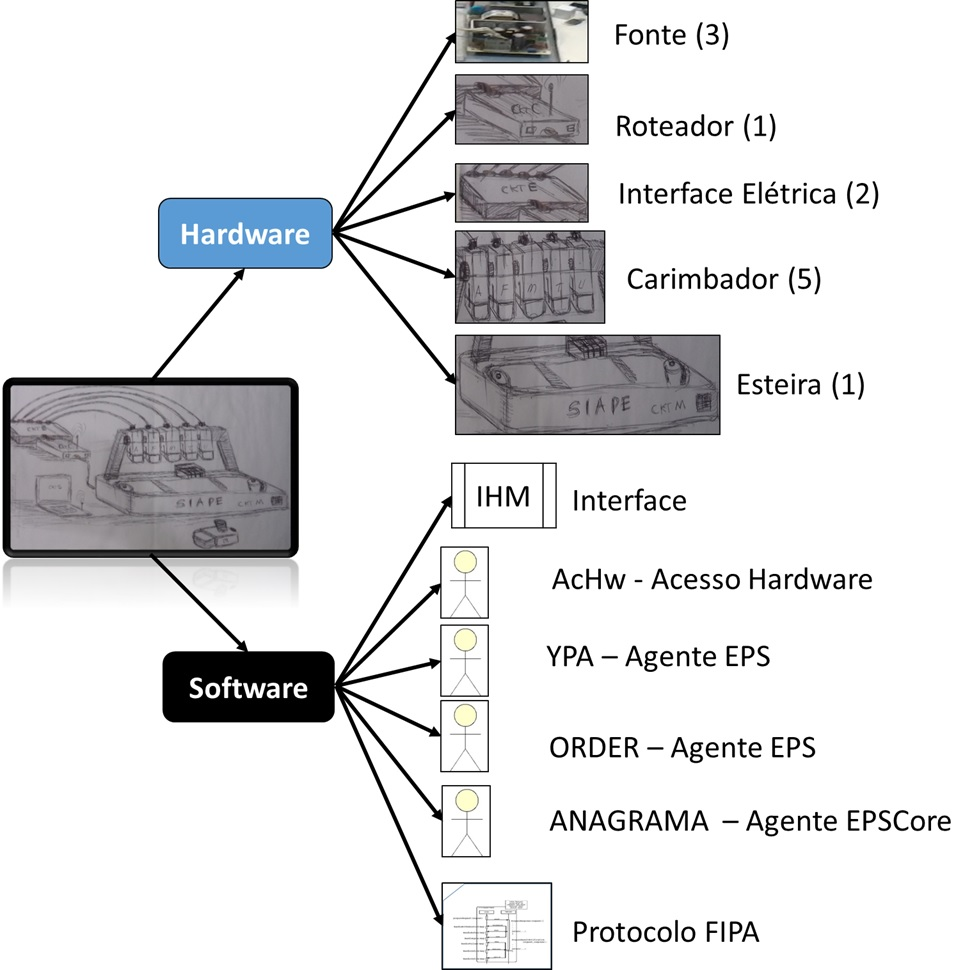
\includegraphics[width=12cm, height=12cm]{F65_SIAPE_HW_SW.jpg} 
	\caption{SIAPE: Módulos de Hardware e Software}
	\label{F65}
\end{figure}

Dos módulos definidos, três não precisaram ser modelados e simulados:

\begin{enumerate}
	\item Módulo Fonte, devido à restrição de 24V e 2A, foram adquiridas fontes que não ultrapassaram esses limites;
	\item Módulo Roteador por estar dentro da faixa de wireless de 2,4Ghz (B+G+N) com uma velocidade de 150 Mbps e uma potência de 700mW;
	\item Módulo Interface Elétrica devido à Placa Raspberry Pi Versão B+ ser aderente à linguagem de programação Java e, portanto, suportar o Framework Jade e compatível à Platafoma Linux. O único quesito não atendido pela Raspberry foi a quantidade de I/Os, e para resolver este problema tornou-se necessária a modelagem e desenvolvimento de uma extensão de I/Os. Essa extensão e os outros módulos encontram-se modelados e simulados na próxima etapa.\par 
\end{enumerate}


\newpage

%=================================== ETAPA 3 ==================================

\subsection{ETAPA 3 - SIMULAÇÕES}
 
Os documentos de requisitos refinados relacionam os Problemas Globais(PG), Regionais (PR) e Locais (PL) com os requisitos refinados. Esses documentos refinados servirão de base para a modelagem e simulação de todas as partes do MESC, a saber: RQRmesc, RQRmes , RQRme, RQRm, RQRe, RQRs, RQRc, RQRA, RQRF, RQRT, RQRU e RQRE. %são base para a a modelagem do sistema. \par 
 	 
As partes atômicas do MESC são submetidas ao processo de modelagem e depois ao processo de simulação. Após a realização desses processos o requisito pode ser aceito como especificação ou pode ser excluído da relação de  requisitos refinados. \par 
 	
Para melhorar o entendimento da visão definida na Etapa 2, com o objetivo de melhorar a realização do processo de modelagem, foi idealizado o caso de uso \textit{realizar um plano}, um diagrama de sequência, um diagrama de atividades e um diagrama de estados para o SIAPE. As Figuras \ref{F60}, \ref{F77}, \ref{F78}  e \ref{F79} ilustram, respectivamente, esses diagramas. Suas descrições encontram-se a seguir.
 	
A Figura \ref{F60} mostra o caso de uso ``Realizar Plano'', onde o Operador insere um pedido no sistema, o agente Order recebe o pedido e solicita informações ao agente YPA para a montagem do agente Anagrama responsável pelo processo produtivo do anagrama. O YPA responde ao Order, este monta o plano com o pedido e instancia o agente Anagrama. Este, por sua vez executa o plano realizando chamadas ao agente AcHw. O AcHw realiza as atividades, \textit{skill} a \textit{skill} e informa o término de cada qual ao Anagrama. O Anagrama, ao seu final, informa ao Order, e morre. O Order, por sua vez, confirma para o Operador a realização do pedido.

\begin{figure}[!h]
	 	\centering
	 	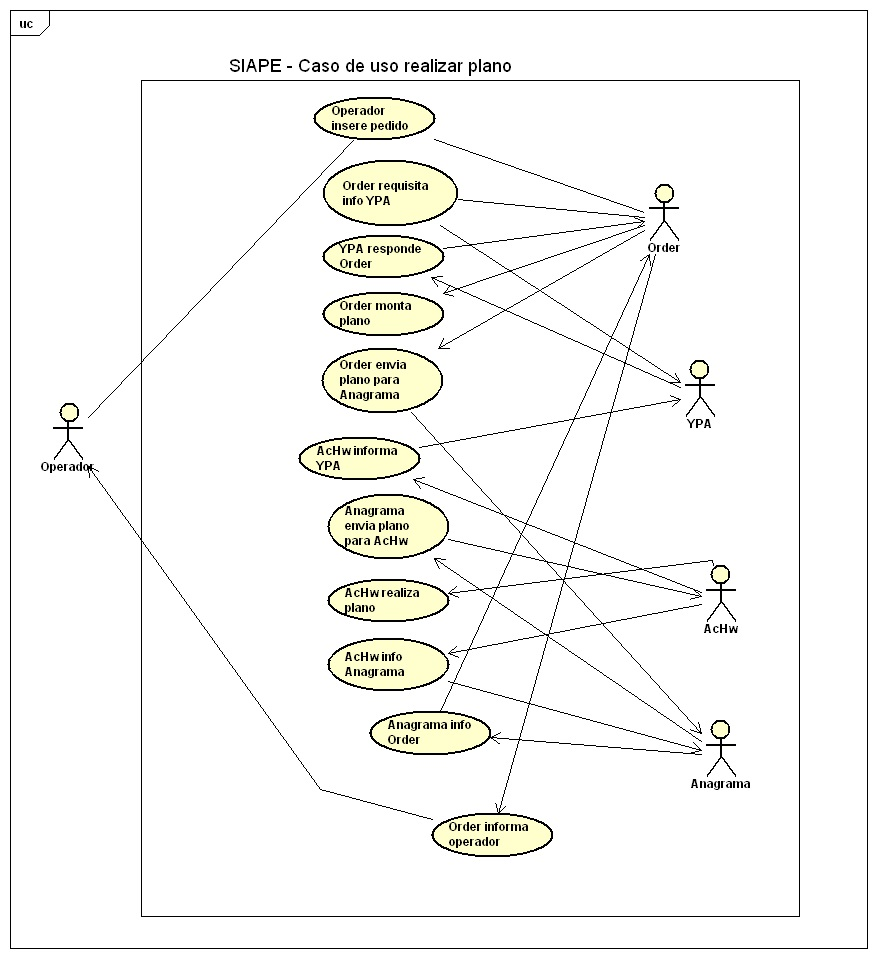
\includegraphics[width=14cm, height=12cm]{F60_SIAPE_CASUSO_PLANO.jpg} 
	 	\caption{Caso de uso: Realizar plano}
	 	\label{F60}
\end{figure}
 		 
A Figura \ref{F77} ilustra uma sequência do ponto de vista do operador. O Operador liga o sistema, o led vermelho é ligado. Em seguida o operador insere o pedido no sistema, carrega o palete na esteira e clica no botão de início de produção. O sistema liga a esteira. O sistema identifica a passagem do palete por meio do sensor, para a esteira e carimba o palete através do acionamento do atuador. Depois, volta a ligar a esteira e prossegue até o fim do plano. O sistema identifica o fim do plano e para a esteira. O operador retira o produto e desliga o sistema. 

\begin{figure}[!h]
 	 	\centering
 	 	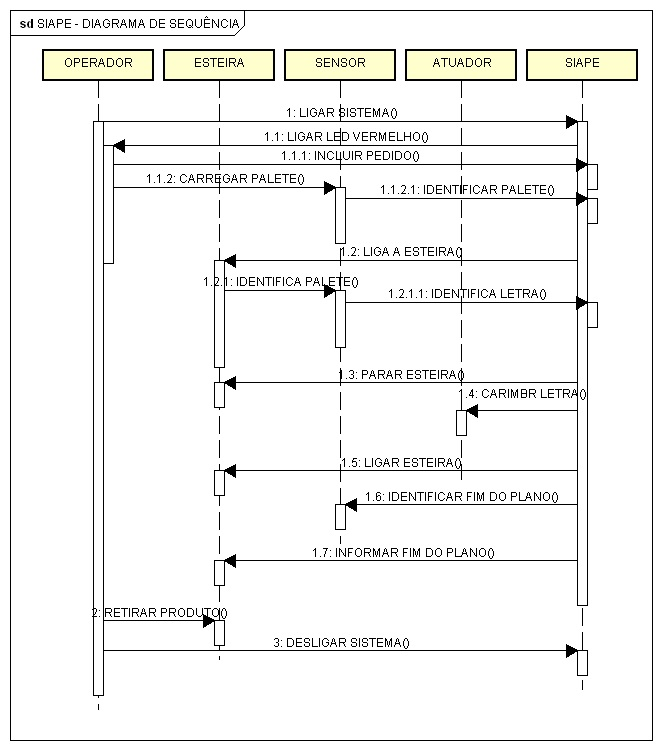
\includegraphics[width=14cm, height=10cm]{F77_SIAPE_DIAGRAMA_SEQUENCIA.jpg} 
 	 	\caption{SIAPE: Diagrama de sequência}
 	 	\label{F77}
\end{figure}
 		 	 
A Figura \ref{F78} ilustra o diagrama de atividades. Esse diagrama também auxilia no entendimento e desenvolvimento do software do sistema. É apenas uma outra visão para os mesmos procedimentos acima descritos. 
 		 	 
\begin{figure}[!h]
	\centering
	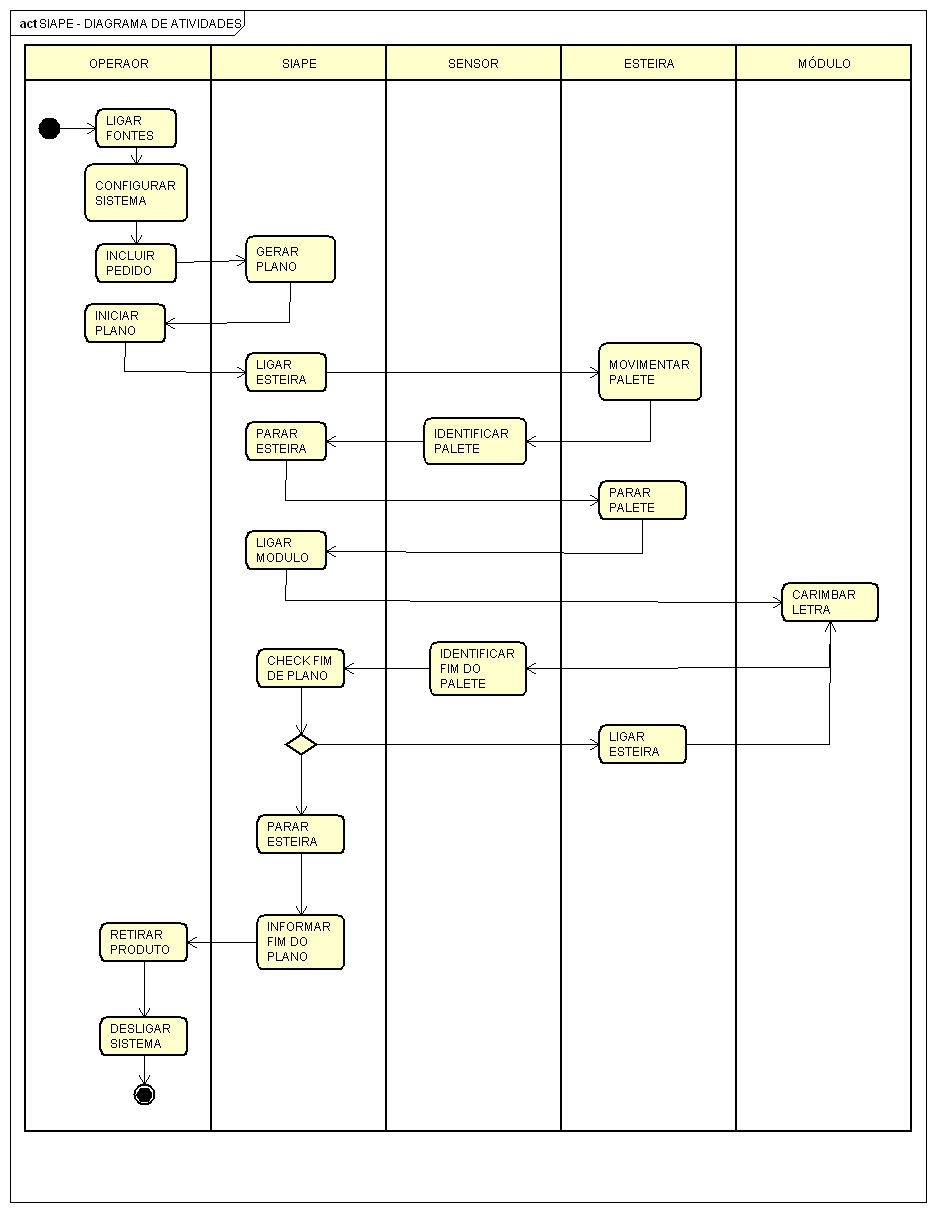
\includegraphics[width=14cm, height=14cm]{F78_SIAPE_DIAGRAMA_ATIVIDADES.jpg} 
	\caption{SIAPE: Diagrama de atividades}
	\label{F78}
\end{figure}
 		 	 	 
 		 	 	
 		 	 	 
 A Figura \ref{F79} ilustra o diagrama de estado do SIAPE que é baseado visão de OMAC para IEC 61131--3~ \cite{OMAC2006}, o qual descreve uma visão sistêmica e padronizada para equipamentos mecatrônicos, quer se trate de parte de uma linha de produção ou de uma máquina completa. Tal diagrama visa mostrar a funcionalidade e dinâmica do sistema.
 
 O diagrama de estado define completamente o estado corrente de uma máquina. As transições entre estados podem ser originados como resultado de uma intervenção  do operador, de uma resposta ao estado de um ou mais objetos de controle ou como resposta de modo completo, definido como a conclusão de todas as etapas que operam dentro de um estado definido. O processo é iniciado com a ligação do sistema e configuração dos dispositivos envolvidos na operação. Uma vez configurado, o sistema entra no modo inativo aguardando que o operador inclua um ou mais pedidos para que um plano de produção seja montado e disponibilizado para a produção. Uma vez que o plano é montado, entra no estado que é responsável por iniciar a produção do plano. O plano pode ser totalmente realizado ou pode ser suspenso para que se inicie outro plano, ou seja, suspenso para alimentação dos recursos de produção na linha. Havendo a suspensão o sistema, pode-se retornar no mesmo ponto de produção onde foi suspenso, ou reiniciado para o início de um novo plano. Também pode ser reiniciado evidenciando que o plano foi totalmente produzido e a operação trata-se de um novo plano sendo produzido. O diagrama também prevê a ocorrência de possíveis erros que são tratados por um processo que aborta a operação, limpa o sistema, pára o processo e uma nova operação pode ser iniciada.    
%
	 
\begin{landscape}
	\begin{figure}
		\centering
		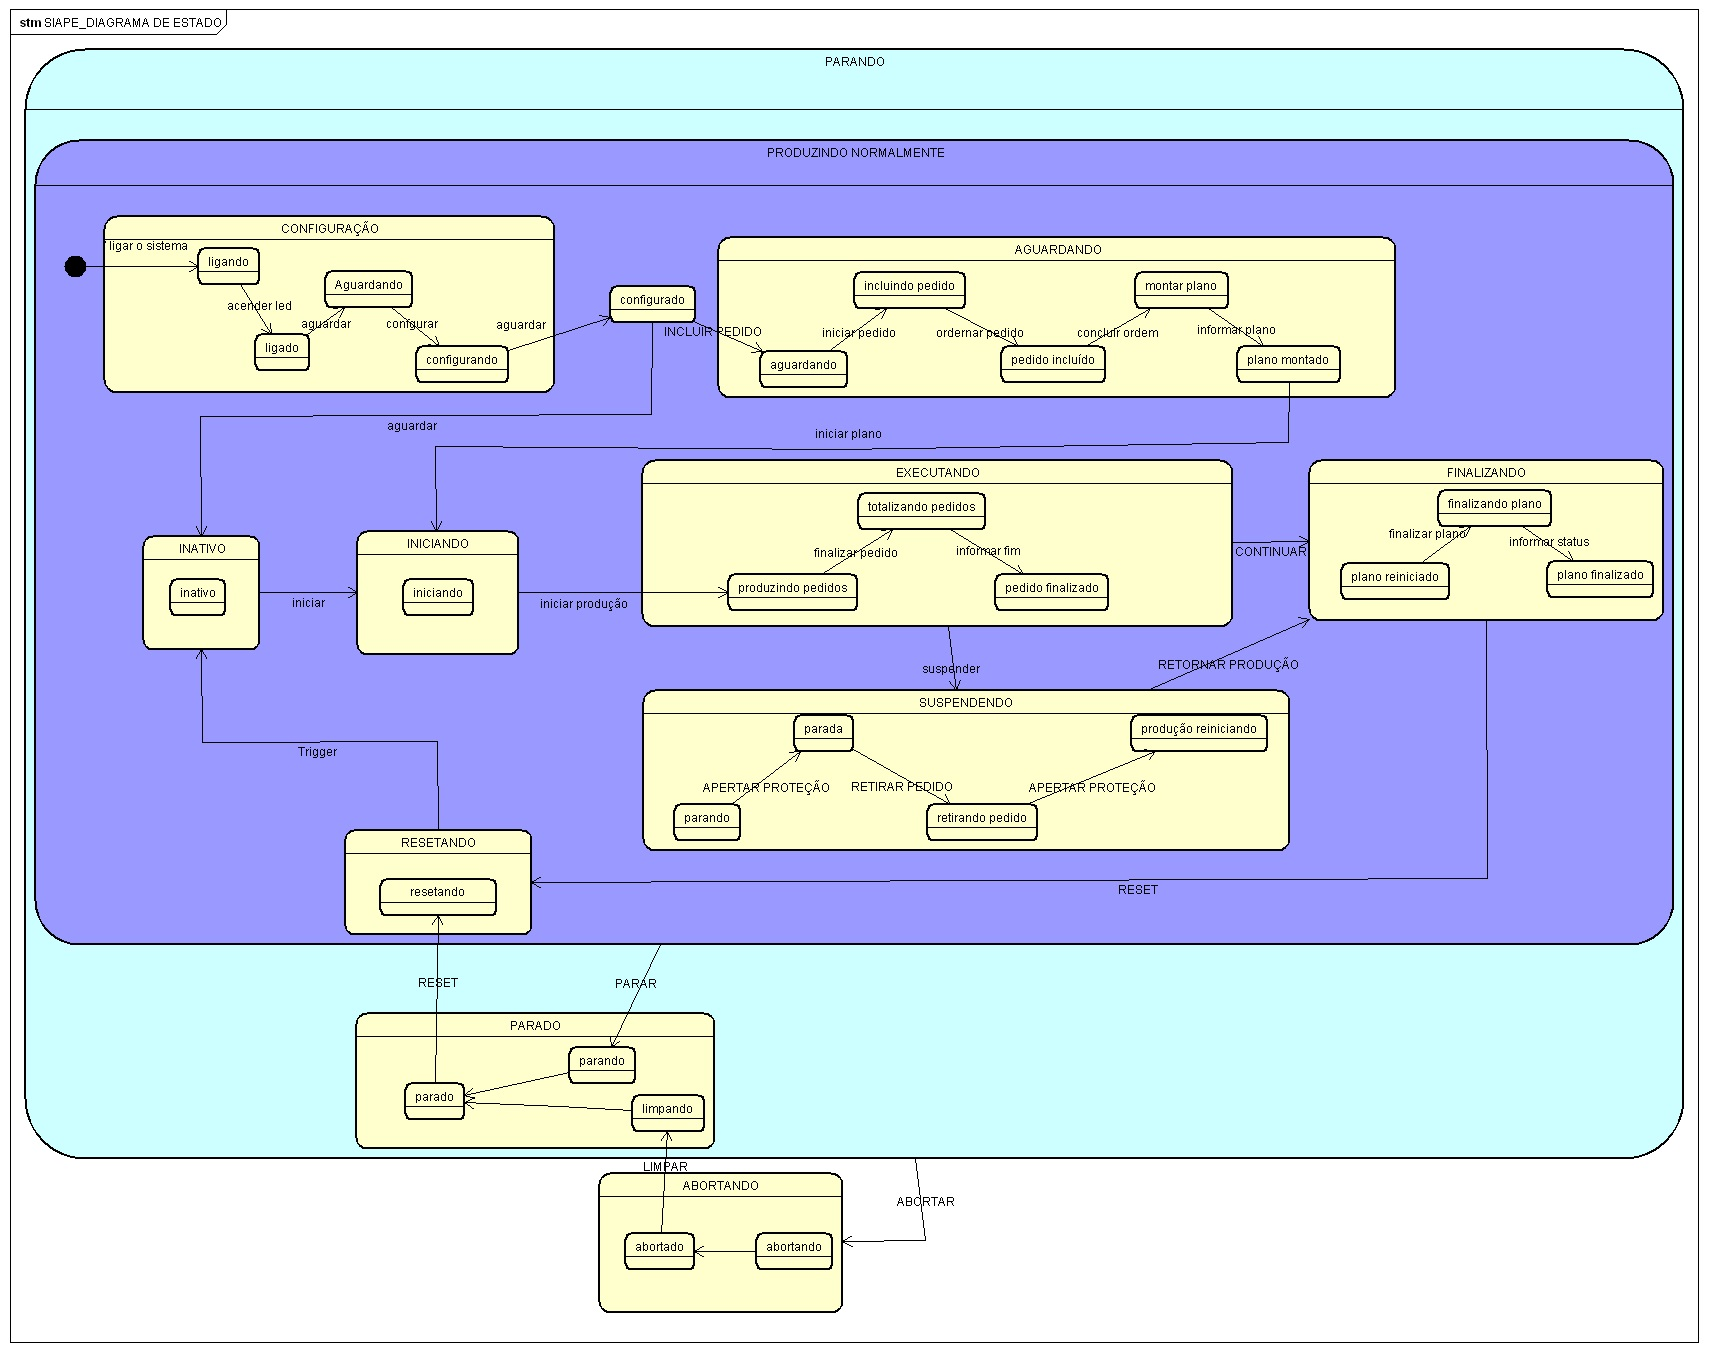
\includegraphics[width=26cm, height=16cm]{F79_SIAPE_DIAGRAMA_ESTADO.jpg} 
		\caption{SIAPE: Diagrama de estados}
		\label{F79}
	\end{figure}
\end{landscape}
 		 
 	A seguir são realizadas breves descrições dos processos de modelagem e simulação para facilitar o entendimento do processo:\par 
  
 	\begin{description}
 	\item [1. Esteira -] 	
 	 O Módulo Esteira foi modelado seguindo as Leis de \textit{Kirchoff} para a parte elétrica, e as Leis de \textit{Hooke} para a parte mecânica. Após a modelagem eletro-mecânica definiu-se a forma da esteira e realizou-se a montagem experimental das partes e  mecânica. A simulação foi realizada e os resultados permitiram a inclusão dos requisitos refinados como especificações técnicas relativas às partes elétricas e mecânicas do módulo. A Figura \ref{F69} ilustra esse processo.
 	 \begin{figure}[!h]
 	 	\centering
 	 	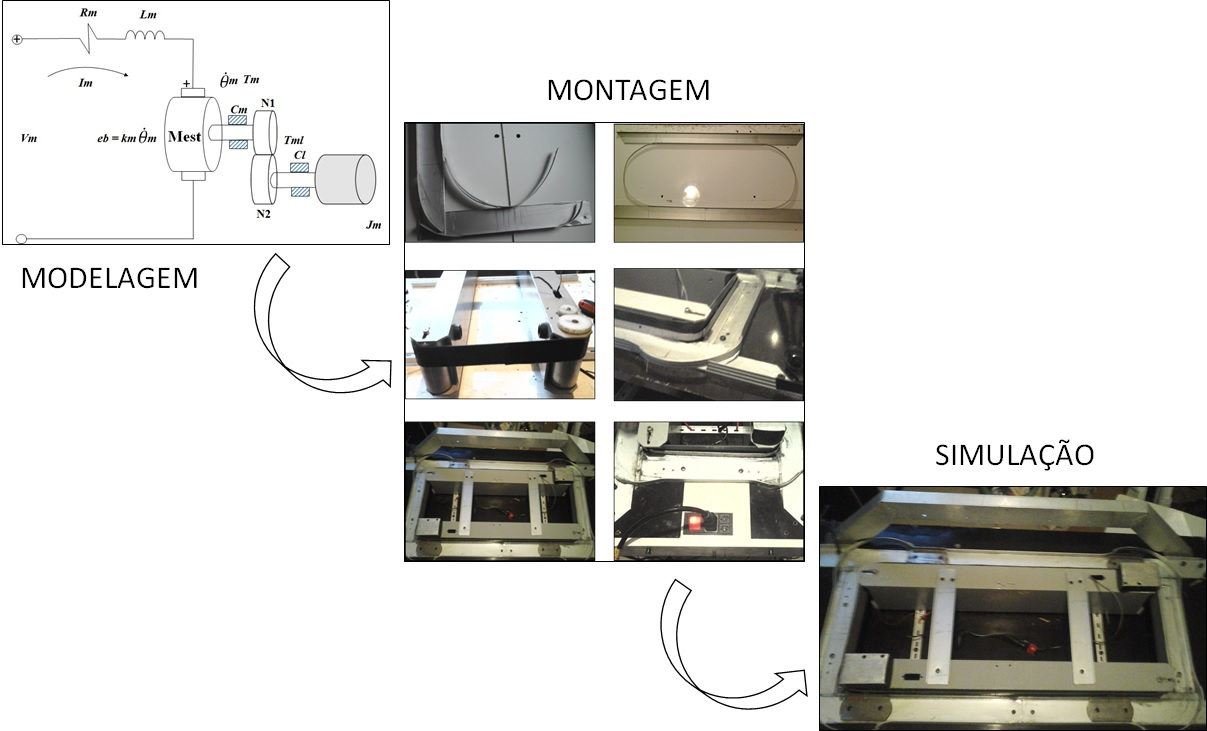
\includegraphics[width=13cm, height=6cm]{F69_SIAPE_ESTEIRA.jpg} 
 	 	\caption{Esteira:  Da modelagem à simulação}
 	 	\label{F69}
 	 \end{figure}
 	 
 	\item[2. Carimbador -]  
 	Da mesma forma que a esteira,  o Módulo Carimbador foi modelado seguindo as Leis de \textit{Kirchoff} para a parte elétrica, e as Leis de \textit{Hooke} para a parte mecânica. Após a modelagem eletro-mecânica definiu-se a forma de um módulo para que fosse realizada a montagem experimental de um módulo. A simulação foi realizada e os resultados permitiram a inclusão dos requisitos refinados como especificações técnicas relativas às partes elétricas e mecânicas do módulo. A Figura \ref{F70} ilustra esse processo.	
 	 \begin{figure}[!h]
 	 	\centering
 	 	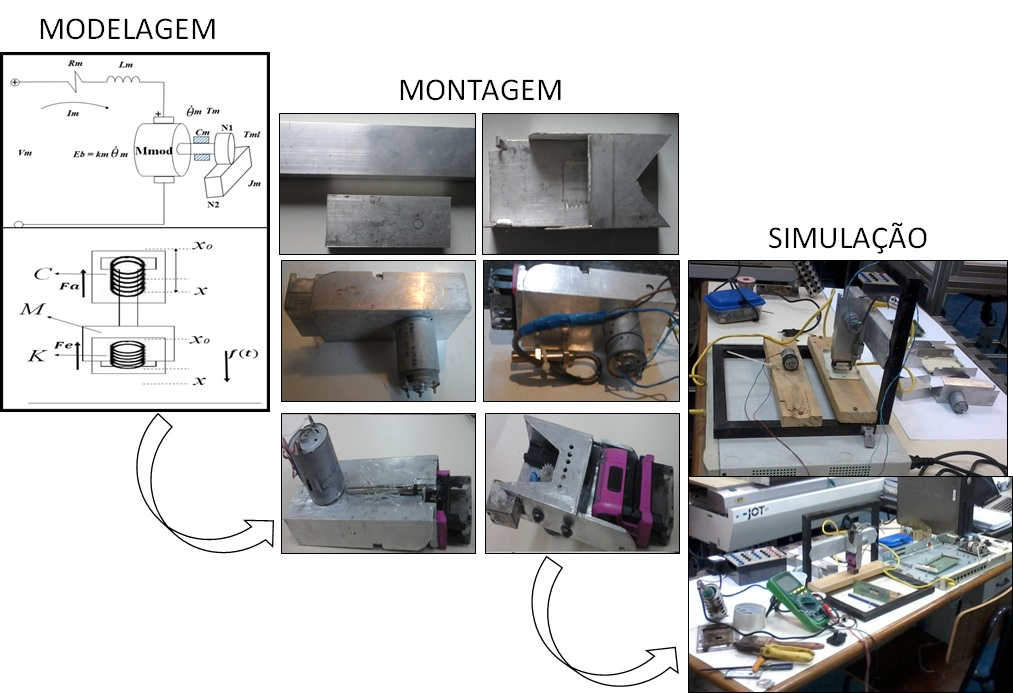
\includegraphics[width=13cm, height=6cm]{F70_SIAPE_MODULO.jpg} 
 	 	\caption{Carimbador: Da modelagem à simulação}
 	 	\label{F70}
 	 \end{figure}
 	 
 	  \item[3. Agente AcHw - ] 
 	  A classe Acesso Hardware foi modelada com a principal função de identificar os módulos que estão presentes no  sistema e disponibilizar para o agente YPA. A Figura \ref{F71} ilustra a criação do código da classe e posterior simulação que evidenciou o seu funcionamento e aprovou sua inclusão como especificação técnica de software.  
 	  \begin{figure}[h]
 	  	\centering
 	  	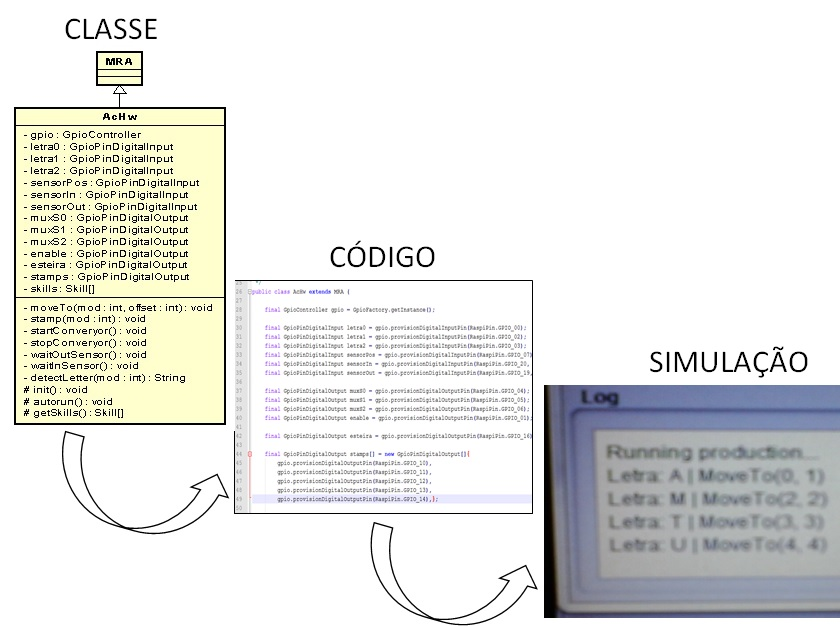
\includegraphics[width=13cm, height=6cm]{F71_SIAPE_CLASSE_ACHW.jpg} 
 	  	\caption{Classe AcHw}
 	  	\label{F71}
 	  \end{figure}
 	  
 	  \item[4. Agente YPA - ]
 	    A classe YPA foi modelada com a principal função de registrar os módulos que estão presentes no  sistema e disponibilizar para o agente Order. A Figura \ref{F72} ilustra a criação do código da classe e posterior simulação que evidenciou o seu funcionamento e aprovou sua inclusão como especificação técnica de software.  
 	  	
 	  \begin{figure}[!h]
 	  	\centering
 	  	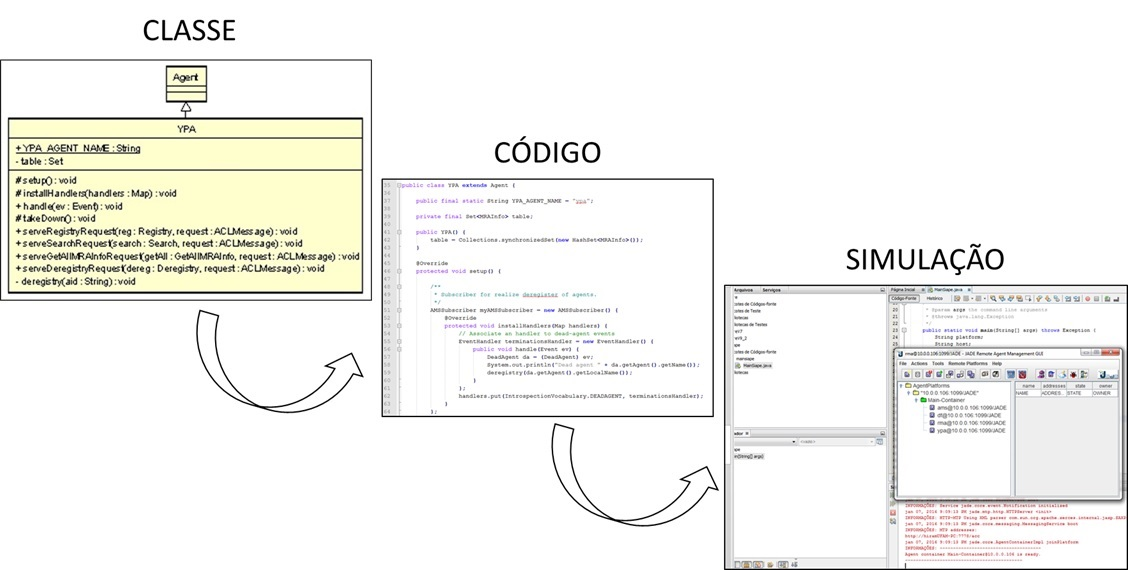
\includegraphics[width=13cm, height=6cm]{F72_SIAPE_CLASSE_YPA.jpg} 
 	  	\caption{Modelagem Classe YPA}
 	  	\label{F72}
 	  \end{figure}
 	  
 	  \item[5. Agente Order - ]  
 	    A classe Order foi modelada com a principal função de montar o plano com os módulos que estão presentes no  sistema e enviar para o agente Anagrama realizar a produção. A Figura \ref{F73} ilustra a criação do diagrama UML e o código da classe e posterior simulação que evidenciou o seu funcionamento e aprovou sua inclusão como especificação técnica de software.  
 	  	
 	  \begin{figure}[!h]
 	  	\centering
 	  	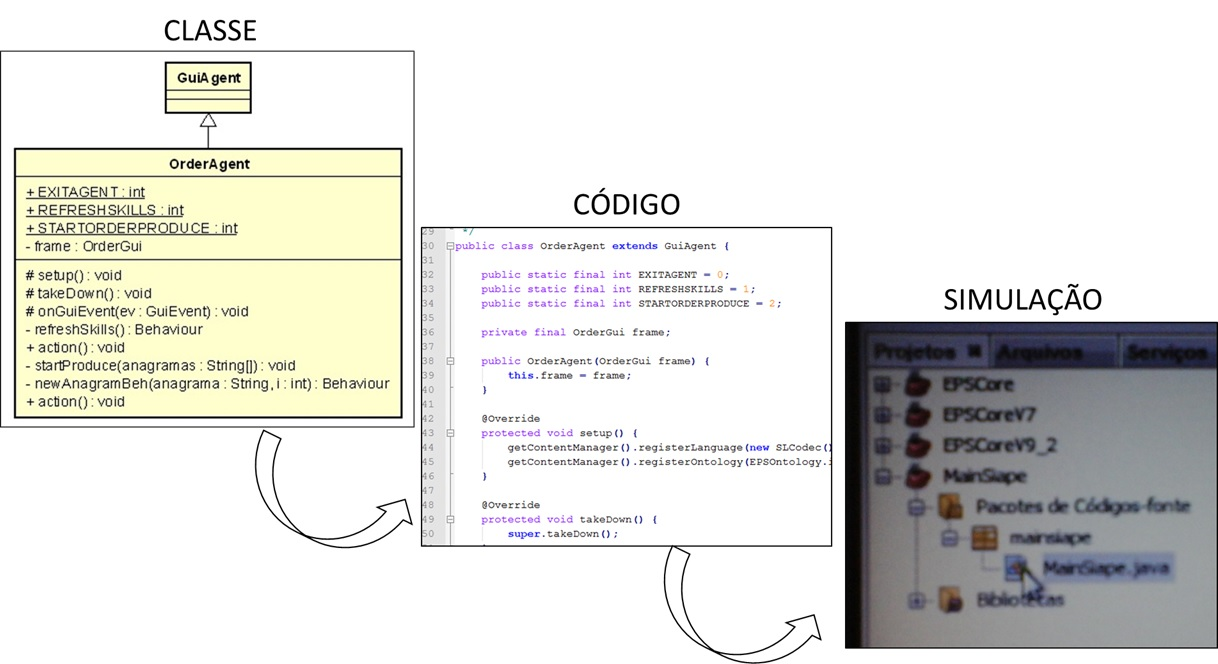
\includegraphics[width=13cm, height=6cm]{F73_SIAPE_CLASSE_ORDER.jpg} 
 	  	\caption{Modelagem classe Order}
 	  	\label{F73}
 	  \end{figure}
 	   	  
 	 \item[6. Agente Anagrama - ] 
 	  A classe Anagrama foi modelada com a principal função de realizar a produção do plano de produção com os módulos presentes no  sistema. A Figura \ref{F74} ilustra a criação do código da classe e posterior simulação que evidenciou o seu funcionamento e aprovou sua inclusão como especificação técnica de software.  
 	 	
 	  \begin{figure}[!h]
 	  	\centering
 	  	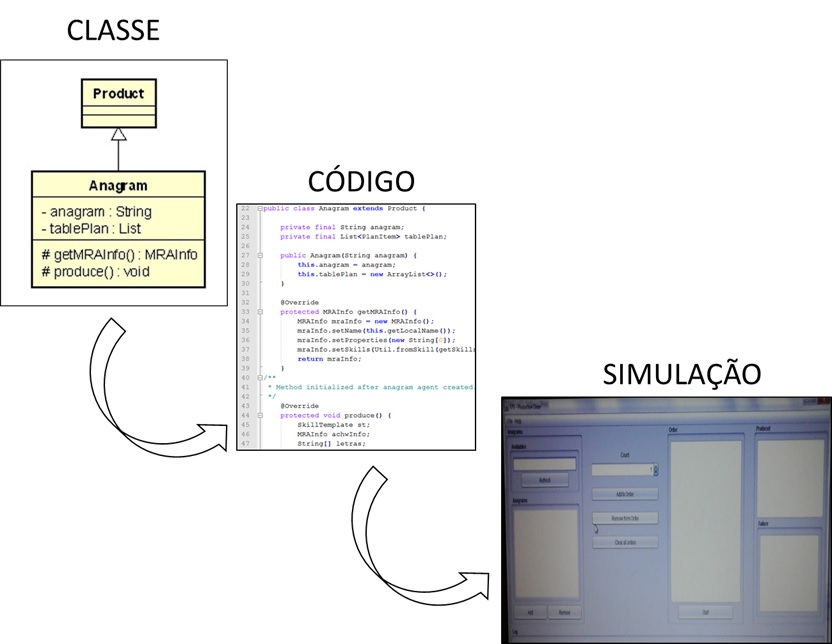
\includegraphics[width=13cm, height=6cm]{F74_SIAPE_CLASSE_ANAGRAMA.jpg} 
 	  	\caption{Modelagem classe Anagrama}
 	  	\label{F74}
 	  \end{figure}
 	  
 	  	  	   	  
 	  \item[7. Protocolo FIPA - ] 
 	  O principal objetivo do Protocolo FIPA é a comunicação entre os agentes do sistema. A Figura \ref{F94} ilustra a criação da classe OrderAgent, um trecho do código e a troca de mensagens capturada pelo agente Sniffer do Framework Jade.  
 	  
 	  
 	   \begin{figure}[!h]
 	   	\centering
 	   	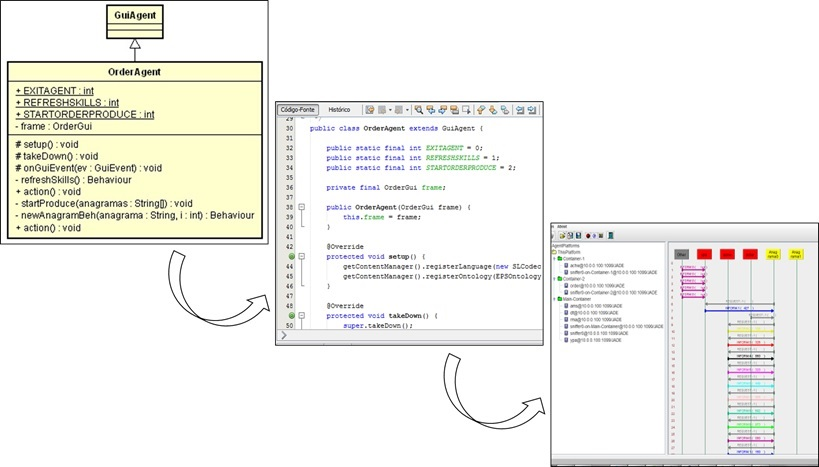
\includegraphics[width=13cm, height=6cm]{F94_SIAPE_FIPA.jpg} 
 	   	\caption{Modelagem Mensagens FIPA}
 	   	\label{F94}
 	   \end{figure}	  
 	\end{description}
 	
 	
 Nesta etapa os requisitos refinados do sistema em forma de problema global (RQRg), na forma regional  (RQRr) e local (RQRl) são modelados e simulados (SimM, SimE, SimS e SimC) até que estes possam ser garantidos como Especificações Técnicas (Et) de cada problema local, a saber: Especificação Técnica Mecânica (EtM), Especificação Técnica Elétrica (EtE), Especificação Técnica de Software (EtS) e Especificação Técnica de Comunicação (EtC). 
 
A Figura \ref{F95} ilustra esse processo para a parte de hardware. Os módulos selecionados com características de hardware foram modelados e rotulados conforme a sua funcionalidade dentro sistema. Esses módulos foram simulados e seus status  foram elevados à categoria de especificações. O significado de cada sigla é explicado a seguir e suas descrições serão realizadas na próxima etapa. 
	\begin{description}
	\begin{figure}[!h]
	\centering
	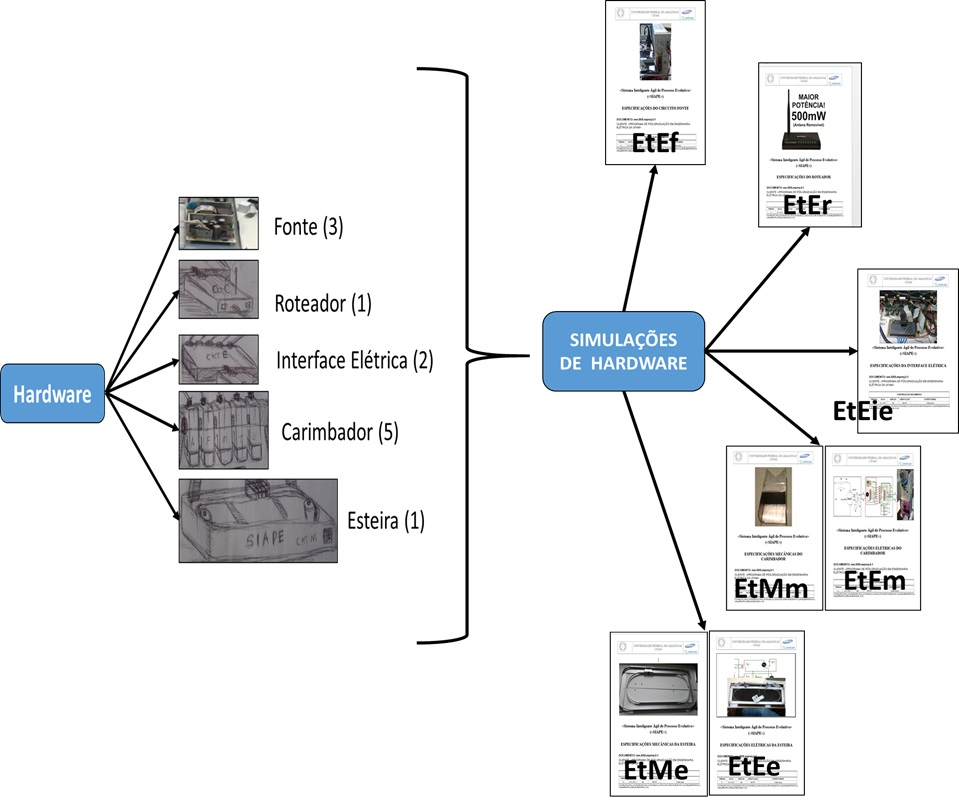
\includegraphics[width=13cm, height=6cm]{F95_SIAPE_SIM_HW.jpg} 
	\caption{Simulação de Hardware}
	\label{F95}
	\end{figure}  
		
		\item[1. EtMm] - Especificação técnica mecânica do módulo;
		\item[2. EtMe] - Especificação técnica mecânica da esteira;
		\item[3. EtEe] - Especificação técnica elétrica da esteira;
		\item[4. EtEf] - Especificação técnica elétrica das fontes;
		\item[5. EtEr] - Especificação técnica elétrica do roteador;
		\item[6. EtEie] - Especificação elétrica da interface elétrica; 
		\item[7. EtEm] - Especificação elétrica do módulo;
		\item[8. EtSis] - Especificação técnica da interface de software.
		
		\end{description}	
		
A Figura \ref{F96} ilustra esse processo para a parte de software. Os módulos selecionados com características de software foram modelados e rotulados conforme a sua funcionalidade dentro do sistema. Esses módulos foram simulados e seus status  foram elevados à categoria de especificações. O significado de cada sigla é explicado a seguir e suas descrições serão realizadas na próxima etapa. 		
		\begin{description}	
	
		 \begin{figure}[!h]
		 	\centering
		 	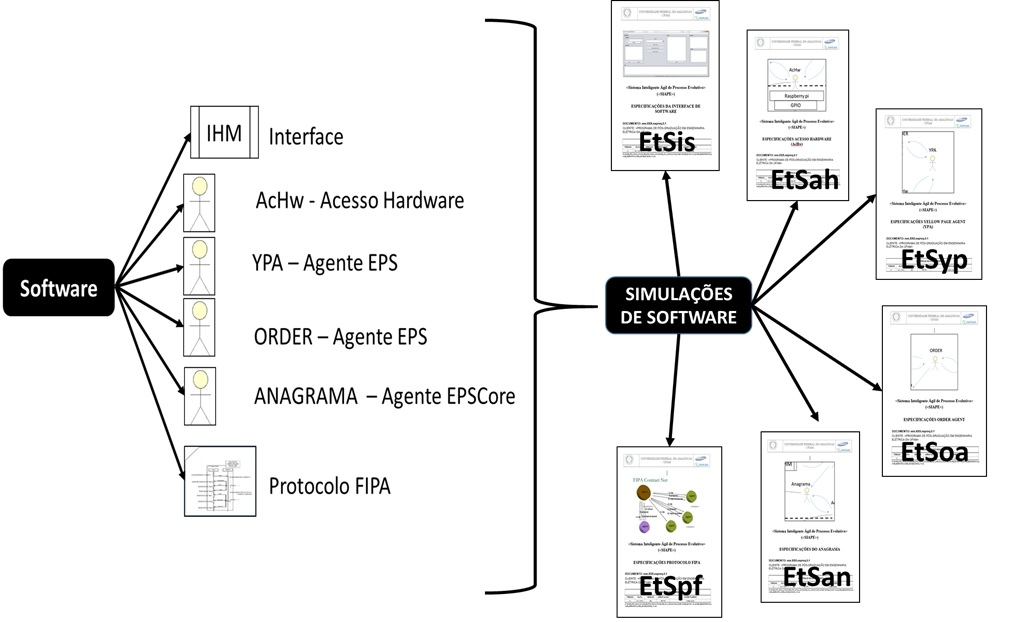
\includegraphics[width=13cm, height=6cm]{F96_SIAPE_SIM_SW.jpg} 
		 	\caption{Simulação de  Software                                                                                                                                                                                                                                                                                                                                                                                                                                                                                                                                                                                                                                                                                                                                                                                                                                                                                                                                                                                                                                                                                                                                                                                                                                                                                                                                     }
		 	\label{F96}
		 \end{figure}

		\item[9. EtSah] - Especificação técnica de software do agente acesso hardware;
		\item[10. EtSyp] - Especificação técnica de software do \textit{Yellow Page Agent(YPA)};
		\item[11. EtSao]  Especificação técnica de software o agente Order;
		\item[12. EtSan] - Especificação técnica de software do agente Anagrama;
		\item[13. EtSpf] - Especificação técnica de software dos protocolos FIPA.	
	\end{description}


 Estas especificações técnicas evidenciam o terceiro marco e servirão de base para do Projeto do Sistema. Na próxima etapa essas especificações serão organizadas no formato de projeto do sistema a ser implementado. 
 
 
  
 %=================================== ETAPA 4 ==================================
 \newpage
 %+++++++++++++++++++++++++++++++++++++++++++++++++++++++
\subsection{ETAPA 4 - PROJETOS}

\begin{description}

\begin{table}[htbp]
	\centering
	\caption{Tabela da etapa 4 - Projetos}
	%=================================================================================================
	\begin{tabular}{|l| p{13.5cm}| c| c| } \hline
		%================================================================================================
		\textbf{Item} 	    & \textbf{Descrição} 
		\\ \hline
		%================================================================================================
		\textbf{1. Objetivos}	   &  
		Integrar as especificações técnicas do sistema no documento de projeto.
		
		\\ \hline
		%================================================================================================
		\textbf{2. Entradas}	  &		
		EtM - Especificações técnicas da parte mecânica, EtE - Especificações técnicas da parte elétrica, EtS - Especificações técnicas da parte de software e EtC - Especificações técnicas da parte de comunicação. \par  	
		
		\\ \hline	
		%================================================================================================	
		\textbf{3. Processo}     &
		As especificações técnicas de hardware e software são organizadas no documento denominado de projeto de sistema.
		
		\\ \hline
		%================================================================================================
		\textbf{4. Saídas}		& 
		\textbf{Documento de Projeto de Sistema contendo as especificações técnicas de hardware, software e requisitos não-funcionais.}  
		
		\\ \hline
		%================================================================================================		
		\textbf{5. Registros}   & 	
		Casos de uso, resultados das simulações, requisitos refinado, requisitos iniciais, requisitos funcionais e não-funcionais. 
		\\ \hline
		%================================================================================================
	\end{tabular}
	\label{T6}\par
	%	Fonte: Hiram Amaral
\end{table}
\item[Descrição textual e visual da etapa] - Para integrar as especificações técnicas - resultado das simulações da Etapa 3 - ao documento de projeto, essas são verificadas por meio dos diagramas de sequência, atividade e estado, pois esses diagramas são partes integrantes do projeto e fazem parte do projeto de classes do sistema. Definidos esses diagramas, eles são consolidados no documento do sistema. \par 		   
As especificações técnicas das partes mecânica, elétrica, de software e de comunicação que servirão de base para a definição dos diagramas a serem desenvolvidos são submetidos ao processo que as transformarão em diagramas de sequência, de atividades e de estado. O resultado é inserido no documento de projeto juntamente com as especificações técnicas de cada parte do sistema. \par 		
O resultado é evidenciado pelo documento de projeto de sistema que serve como evidência da entrega do quarto marco. 


\end{description}


		  \begin{figure}[!h]
		  	\centering
		  	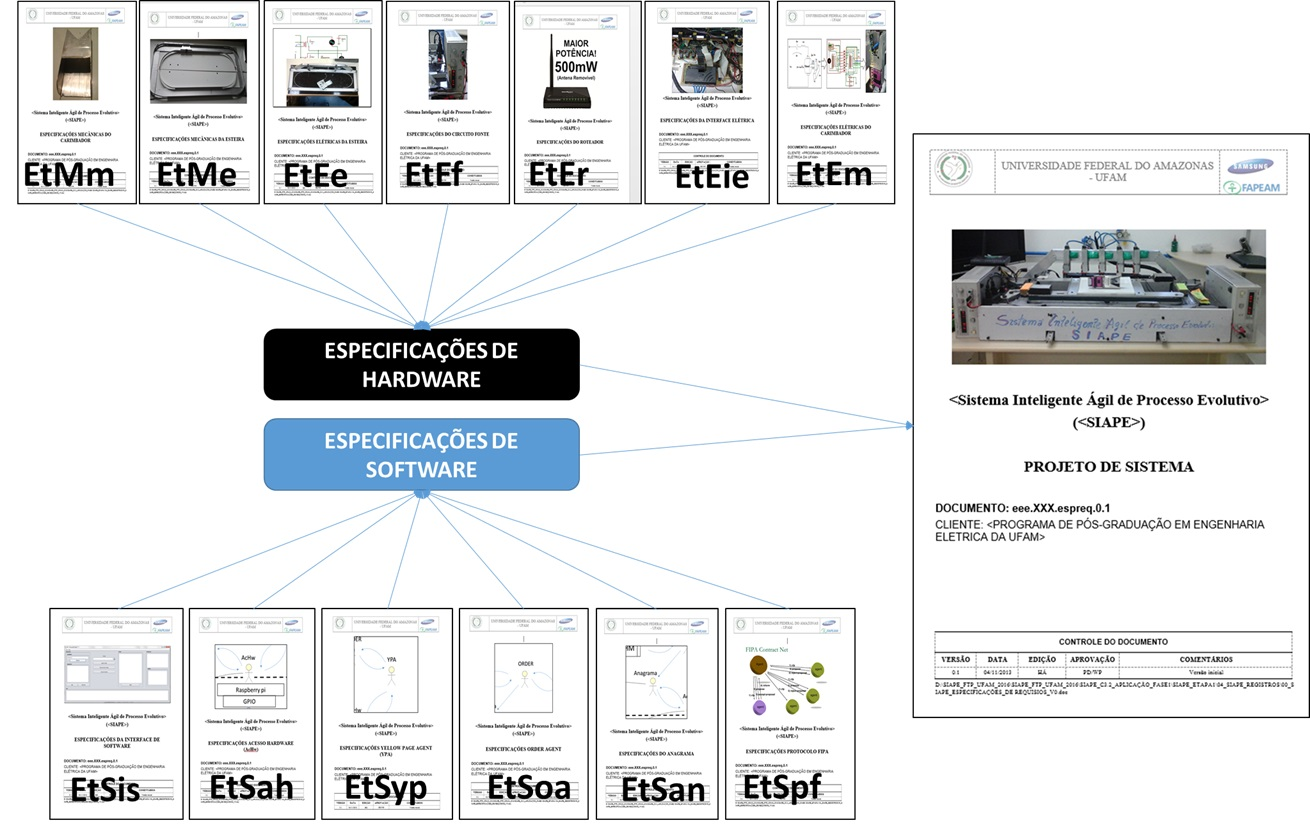
\includegraphics[width=16cm, height=10cm]{F80_SIAPE_PROJETO_SISTEMA.jpg} 
		  	\caption{Projeto de Sistema}
		  	\label{F80}
		  \end{figure}
		  
A Figura \ref{F80} ilustra a consolidação das especificações de hardware e software no documento do Projeto de Sistema. As descrições das especificações são relacionadas a seguir:
	 		\begin{description}
	 			\item[1. EtMm] - Especificação técnica mecânica define as medidas que deverão ser realizadas no material especificado para transformá-lo no protótipo mecânico do módulo;
	 			\item[2. EtMe] - Especificação técnica mecânica da esteira de define a forma que deverá ser desenvolvida para que o palete trafegue sem interferências;
	 			\item[3. EtEe] - Especificação elétrica da esteira define a alimentação do motor em valores de tensão e corrente que não devem ultrapassar os valores definidos como restrições para o projeto;
	 			\item[4. EtEf] - Especificação técnica elétrica das fontes especifica os valores de tensão e corrente para todos todo os módulos do sistema, e que atendem às restrições;
	 			\item[5. EtEr] - Especificação elétrica do roteador descreve os dados técnicos do roteador que serão utilizados para conectar os dispositivo do SIAPE;
	 			\item[6. EtEie] -  Especificação elétrica da interface elétrica define todos os componentes e circuitos elétricos que deverão ser implementados no sistema;
	 			\item[7. EtEm] - Especificação elétrica do módulo define os circuitos elétricos e que deverão ser implementados;
	 			\item[8. EtSis] - Especificação técnica de software da interface de software do sistema descreve os campos que devem ser implementados no sistema.
	 			\item[9. EtSah] - Especificação técnica de software descreve as características e habilidades do agente de acesso hardware;
	 			\item[10. EtSyp] - Especificação técnica de software descreve as características e habilidades do agente de Yellow Page Agent (YPA);
	 			\item[11. EtSao] - Especificação técnica de software descreve as características e habilidades do agente Order;
	 			\item[12. EtSan] - Especificação técnica de software descreve as características e habilidades do agente Anagrama;
	 			\item[13. EtSpf] - Especificação técnica de software descreve todos os protocolos utilizados no SIAPE. 		
	 		\end{description}

O Projeto de Sistema evidencia o quarto marco e contém as especificações que expressam o resultado de estudos que iniciaram com as necessidades do cliente, os referenciais internos e externos. Esses foram transformados em requisitos refinados, modelados e simulados para que as especificações pudessem ser garantidas como tal. Na Etapa 5 o Projeto de Sistema é implementado.

%=================================== ETAPA 5 ==================================

\clearpage
%+++++++++++++++++++++++++++++++++++++++++++++++++++++++
\subsection{ETAPA 5 - IMPLEMENTAÇÕES}

\begin{table}[htbp]
	\centering
	\caption{Tabela da etapa 5 - Implementações}
	%=================================================================================================
	\begin{tabular}{|l| p{13.5cm}| c| c| } \hline
		%================================================================================================
		\textbf{Item} 	    & \textbf{Descrição} 
		\\ \hline
		%================================================================================================
		\textbf{1.Objetivos}	   &  
		Implementar os projetos definidos na Etapa 4.
		\\ \hline
		%================================================================================================
		\textbf{2.Entradas}	  &		
		
		Projeto de hardware contendo os módulos mecânicos e elétricos.\par  	
		Projeto de software contendo os módulos de software e de comunicação. 
		\\ \hline	
		%================================================================================================	
		\textbf{3.Processo}     &
		Os projetos são implementados e transformados em protótipos das partes do sistema.
		\\ \hline
		%================================================================================================
		\textbf{4.Saídas}		& 
		Protótipo elétrico, protótipo mecânico, códigos do software e de comunicação.
		\\ \hline
		%================================================================================================		
		\textbf{5.Registros}   & 	
		Diagramas de classe, diagrama de sequência, diagrama de atividades, diagrama de estado, esquema elétrico e especificações técnicas.
		\\ \hline
		%================================================================================================
	\end{tabular}
	\label{T7}\par
	%	Fonte: Hiram Amaral
\end{table}

	\begin{description}
		
		\item[Descrição textual e visual da etapa] - A partir das especificações técnicas são desenvolvidos circuitos que atendam às especificações. Desses circuitos são originados os esquemas elétricos, as placas de circuito impresso (PCI) e são acoplados aos seus respectivos módulos. \par 
		
		
		\item[1. EtMm] - A especificação técnica mecânica define as medidas que deverão ser realizadas no material especificado para transformá-lo no protótipo mecânico do módulo;\par 
		
		  \begin{figure}[!h]
		  	\centering
		  	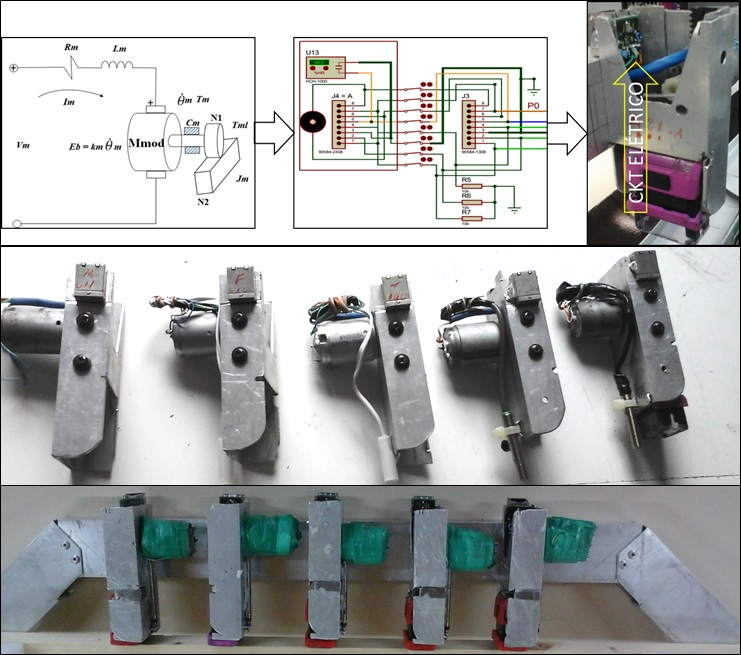
\includegraphics[width=13cm, height=9cm]{F81_SIAPE_MODULOS_LETRAS.jpg} 
		  	\caption{Evolução dos módulos: do circuito elétrico aos módulos}
		  	\label{F81}
		  \end{figure}
				
		\item[2. EtMe] - A especificação técnica mecânica da esteira de define a forma que deverá ser desenvolvida para que o palete trafegue sem interferências; \par 	
	
	 \begin{figure}[!h]
	 	\centering
	 	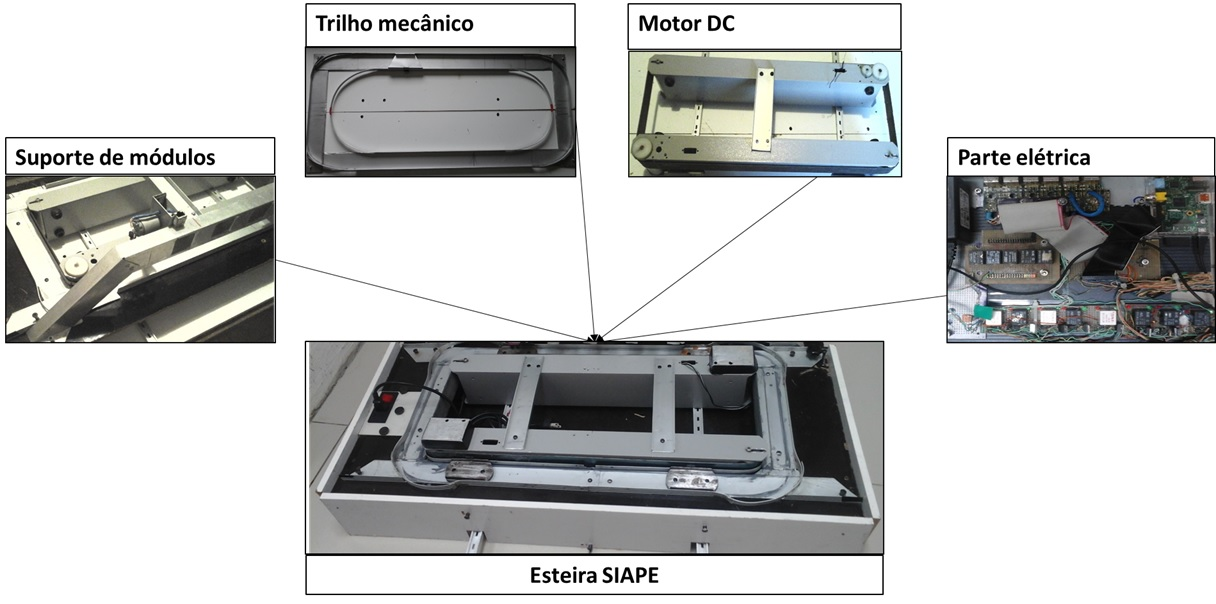
\includegraphics[width=13cm, height=5cm]{F82_SIAPE_ESTEIRA.jpg} 
	 	\caption{Evolução da esteira: do modelo ao protótipo}
	 	\label{F82}
	 \end{figure}
	
		\item[3. EtEe] - A especificação elétrica da esteira define a alimentação do motor em valores de tensão e corrente que não devem ultrapassar os valores definidos como restrições para o projeto;
		 
		 \begin{figure}[!h]
		 	\centering
		 	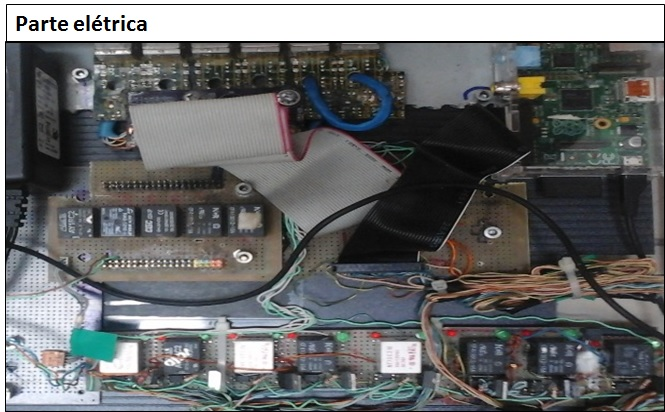
\includegraphics[width=12cm, height=5cm]{F83_SIAPE_PARTE_E.jpg} 
		 	\caption{SIAPE : Parte elétrica}
		 	\label{F83}
		 \end{figure}				
		
		\item[4. EtEf] - A especificação técnica elétrica das fontes especifica os valores de tensão e corrente para todos todo os módulos do sistema, e que atendem às restrições;
			 
			 \begin{figure}[!h]
			 	\centering
			 	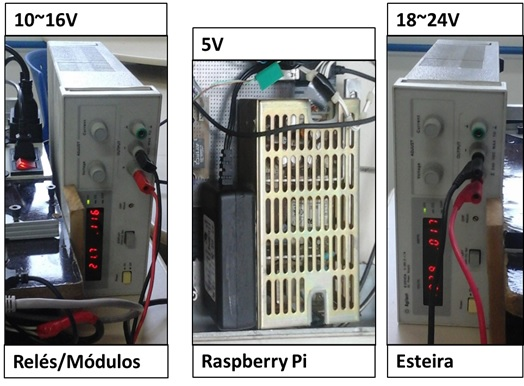
\includegraphics[width=11cm, height=5cm]{F84_SIAPE_FONTES.jpg} 
			 	\caption{SIAPE : Fontes}
			 	\label{F84}
			 \end{figure}
		
		\item[5. EtEr] - A especificação elétrica do roteador descreve os dados técnicos do roteador que serão utilizados para conectar os dispositivo do SIAPE;
		
		
			 \begin{figure}[!h]
			 	\centering
			 	\includegraphics[width=11cm, height=4cm]{F85_SIAPE_ROTEADOR.jpg} 
			 	\caption{SIAPE : Roteador}
			 	\label{F85}
			 \end{figure}
		
		\item[6. EtEie] -  A especificação elétrica da interface elétrica define todos os componentes e circuitos elétricos que deverão ser implementados no sistema;
		
		
		 \begin{figure}[!h]
		 	\centering
		 	\includegraphics[width=10cm, height=5cm]{F86_SIAPE_INTERFACE_ELETRICA.jpg} 
		 	\caption{SIAPE : Interface elétrica}
		 	\label{F86}
		 \end{figure}
		
		\item[7. EtEm] - A especificação elétrica do módulo define os circuitos elétricos e que deverão ser implementados;
		
		 \begin{figure}[!h]
		 	\centering
		 	\includegraphics[width=8cm, height=5cm]{F87_SIAPE_ELETRICA_MOD.jpg} 
		 	\caption{SIAPE : Circuito elétrico módulo }
		 	\label{F87}
		 \end{figure}
		
		
		\item[8. EtSis] - A especificação técnica de software da interface de software do sistema descreve os campos que devem ser implementados no sistema.

		 \begin{figure}[!h]
		 	\centering
		 	\includegraphics[width=14cm, height=7cm]{F88_SIAPE_INTERFACE.jpg} 
		 	\caption{SIAPE : Interface}
		    \label{F88}
		 \end{figure}

		\item[9. EtSah] - A especificação técnica de software descreve as características e habilidades do agente de acesso hardware;
			
		 \begin{figure}[!h]
		 	\centering
		 	\includegraphics[width=14cm, height=7cm]{F89_SIAPE_ACHW.jpg} 
		 	\caption{SIAPE : Acesso Hardware}
		 	\label{F89}
		 \end{figure}
		
		\item[10. EtSyp] - A especificação técnica de software descreve as características e habilidades do agente de Yellow Page Agent(YPA);
		
		 \begin{figure}[!h]
		 	\centering
		 	\includegraphics[width=14cm, height=7cm]{F90_SIAPE_YPA.jpg} 
		 	\caption{SIAPE: YPA}
		 	\label{F90}
		 \end{figure}	
				
		\item[11. EtSao] - A especificação técnica de software descreve as características e habilidades do agente Order;
				
		 \begin{figure}[!h]
		 	\centering
		 	\includegraphics[width=14cm, height=7cm]{F91_SIAPE_ORDER.jpg} 
		 	\caption{SIAPE: ORDER}
		 	\label{F91}
		 \end{figure}			
		
		\item[12. EtSan] - A especificação técnica de software descreve as características e habilidades do agente Anagrama;
		
	 \begin{figure}[!h]
	 	\centering
	 	\includegraphics[width=14cm, height=7cm]{F91_SIAPE_ORDER.jpg} 
	 	\caption{SIAPE: ANAGRAMA}
	 	\label{F92}
	 \end{figure}			
		
		\item[13. EtSpf] - A especificação técnica de software descreve todos os protocolos utilizados no SIAPE.	
	\end{description}


Cada módulo é denominado com um nome de protótipo da parte específica do sistema. Estes módulos seguem para a Etapa 6 onde deverão ser testados contra as especificações técnicas e requisitos refinados.  

%=================================== ETAPA 6 ==================================

\clearpage
%+++++++++++++++++++++++++++++++++++++++++++++++++++++++
\subsection{ETAPA 6 - TESTES}

\begin{table}[htbp]
	\centering
	\caption{Tabela da etapa 6 - Testes}
	%=================================================================================================
	\begin{tabular}{|l| p{13.5cm}| c| c| } \hline
		%================================================================================================
		\textbf{Item} 	    & \textbf{Descrição} 
		\\ \hline
		%================================================================================================
		\textbf{1.Objetivos}	   &  
		Testar os protótipos implementados na Etapa 5.
		\\ \hline
		%================================================================================================
		\textbf{2.Entradas}	  &		
		Protótipo mecânico, protótipo elétrico, códigos do software, protocolos de comunicação FIPA. 
		\\ \hline	
		%================================================================================================	
		\textbf{3.Processo}     &
		Os protótipos funcionais implementados na Etapa 5 são submetidos aos testes especificados nos RQRs e Ets.
		\\ \hline
		%================================================================================================
		\textbf{4.Saídas}		& 
		Protótipo mecânico testado, protótipo elétrico testado, códigos do software testados, protocolos de comunicação FIPA testados.  	
		\\ \hline
		%================================================================================================		
		\textbf{5.Registros}   & 	
		RQRs, Ets, resultados dos testes.
		\\ \hline
		%================================================================================================
	\end{tabular}	
	\label{T8}\par
	%	Fonte: Hiram Amaral
\end{table}

\begin{description}
	
\item[Descrição textual e visual da etapa] - Os protótipos funcionais são submetidos aos testes especificados, individualmente, com o objetivo de testar sua funcionalidade contra os requisitos refinados e contra as especificações.\par 
Havendo a aprovação dos testes, os protótipos assumem o status de protótipos aprovados e preparados para serem integrados.

\end{description}

Na Figura \ref{F97} pode ser visualizado um resumo dos testes aplicados às partes ou ao todo durante a Etapa. As descrições encontram-se a seguir de acordo com a numeração:
	\begin{description}
		\item[ Número 1 ] - Este teste objetiva testar a funcionalidade do motor, o trajeto da esteira e a robustez do módulo mecânico da esteira. A alimentação de corrente é aplicada diretamente ao motor DC, neste caso variando a tensão entre os limites de 10V a 16V.  

	\begin{figure}[h]
		\centering
		\includegraphics[width=16cm, height=7cm]{F97_SIAPE_TESTES.jpg} 
		\caption{Etapa de testes}
		\label{F97}
	\end{figure}

	\item[ Número 2 ] - Da mesma forma que foi aplicado à esteira, este teste objetiva testar a funcionalidade do motor, o trajeto do carimbo e a robustez do módulo mecânico das letras. A alimentação de corrente é aplicado diretamente ao motor DC, neste caso variando a tensão entre os limites de 16V a 24V;

	\item[ Número 3 ] - Este teste objetiva testar a funcionalidade do módulo eletro-mecânico através do comando do software.  Três maneiras podem ser utilizadas para realizar este teste: Utilizar os comando por meio do PC (Número 7) aplicados diretamente à interface elétrica, ou por meio dos números 6, 5, 4, e 3, ou ainda por meio dos números 8, 4 e 3. Percebe-se uma entidade MES é realizada;  
	
	\item[ Número 4 ] - O PC acessa a interface elétrica via roteador e manda os comandos para o módulo ME. Há que se perceber que, também neste caso, uma entidade MES é realizada;
	
	
	\item[ Número 5 ] - O PC acessa a interface elétrica via roteador e protocolo FIPA, e manda os comandos para o módulo ME. Há que se perceber que, neste caso, uma entidade MESC é realizada;	
	
	\item[ Número 6 ] - O PC acessa a interface elétrica via roteador e manda os comandos para o módulo ME. Idêntico ao teste número 6;
	
	\item[ Número 7 ] - O PC acessa a interface elétrica e manda os comandos para o módulo ME. Há que se perceber que, também neste caso, uma entidade MES é realizada;
	
	\item[ Número 8 ] - O PC acessa a interface elétrica via roteador e manda os comandos para o módulo ME. Há que se perceber que, também neste caso, uma entidade MESC é realizada;
	
	\item[ Número 9 ] - O PC acessa a interface elétrica e manda os comandos para o módulo ME da esteira. Há que se perceber que, também neste caso, uma entidade MES é realizada;


	\end{description}
	

	
A entrega dessas partes testadas evidencia a entrega do sexto marco. 
	
O resultado dessa etapa é o conjunto de partes individuais do sistema testadas e aprovadas para serem submetidas ao processo de integração na Etapa 7.\par





%=================================== ETAPA 7 ==================================
\clearpage
%+++++++++++++++++++++++++++++++++++++++++++++++++++++++
\subsection{ETAPA 7 - INTEGRAÇÃO MODULAR  E VALIDAÇÃO}

\begin{table}[htbp]
	\centering
	\caption{Tabela da etapa 7 - Integração modular e validação}
	%=================================================================================================
	\begin{tabular}{|l| p{13.5cm}| c| c| } \hline
		%================================================================================================
		\textbf{Item} 	    & \textbf{Descrição} 
		\\ \hline
		%================================================================================================
		\textbf{1.Objetivos}	   &  
		Integrar as partes aprovadas e e validar a integração.
		\\ \hline
		%================================================================================================
		\textbf{2.Entradas}	  &		
		 Protótipo mecânico testado,  protótipo elétrico testado,  códigos testado e protocolos testados.
		\\ \hline	
		%================================================================================================	
		\textbf{3.Processo}     &
		Protótipos testados são submetidos ao processo de integração e validação.
		\\ \hline
		%================================================================================================
		\textbf{4.Saídas}		& 
		Partes M, E, S e C integradas e validadas e preparadas para validação sistêmica. 
		\\ \hline
		%================================================================================================		
		\textbf{5.Registros}   & 
		Resultados dos testes e validações realizadas.
		\\ \hline
		%================================================================================================
	\end{tabular}
	\label{T9}\par
	%	Fonte: Hiram Amaral
\end{table}

\begin{description}
\item[Descrição textual e visual da etapa] - Os protótipos testados e aprovados são submetidos ao processo de integração de suas partes atômicas. \par 
Os protótipos M e E originam a parte integrada ME com suas características específicas, por exemplo, a parte mecânica é móvel e pode ser movida manualmente. A parte elétrica montada fornece as tensões para alimentar o motor. Ao se integrar essas partes, M e E produz-se uma entidade que pode ser alimentada eletricamente para que seja gerado um movimento eletro-mecânico. Ao se integrar a parte S à entidade ME, têm-se uma entidade ME automatizada. E finalmente, ao se integrar a parte C, ter-se-á uma entidade mecatrônica com suas características específicas.


\end{description}


\begin{figure}[h]
	\centering
	\includegraphics[width=16cm, height=7cm]{F98_SIAPE_INTEGRACAO_MODULAR.jpg} 
	\caption{Etapa de integração modular e validação}
	\label{F98}
\end{figure}


A Figura \ref{F98} ilustra a integração das partes Mecânicas, Eletrônicas, de Software e de Comunicação  e a realização do MESC. Essa integração modular é validada por meio da aplicação dos testes de números 1 a 9 da etapa anterior (Etapa 6). A diferença é que agora os módulos encontram-se integrados e todos os comandos são realizados no PC, e todos os dispositivos devem ser ligados à rede para que o protótipo MESC seja validado modularmente. Outra questão a ser observada é que os requisitos e especificações, neste estágio, são mais rígidos e devem ser tratados antes que o sistema siga para a integração validação sistêmica.    


Uma das validações é ilustrada na Figura \ref{F102} que valida tanto a parte de software quanto a parte de hardware na detecção de desconexão de módulos. Essa atividade é fundamental para a evidência do conceito \textit{plug and produce} durante a aplicação do estudo de caso no Capítulo 4. No detalhe tem-se do lado esquerdo, o sistema funcionando com todos os módulos, e a interface IDE retornando com todos as letras, no centro, tem-se desconexão do módulo. Do lado direito, em tempo real tem-se o sistema identificando a atividade e retornando a informação N.C. (não conectado).

 \begin{figure}[h]
 	\centering
 	\includegraphics[width=16cm, height=7cm]{F102_SIAPE_DESCONEXAO.jpg} 
 	\caption{Detecção de desconexão de módulos}
 	\label{F102}
 \end{figure}


Além da rigidez na realização da validação modular, este também é o momento para organizar o material que será disponibilizado para o cliente e para os especialistas que irão ficar responsáveis pelo sistema, isto é, é o momento de finalizar os manuais técnico e de usuário. Esses manuais deverão ter suas eficácias postas à prova durante a Etapa de Comissionamento, isso para que potenciais erros possam ser identificados e evitem interferências no sistema quando da sua utilização pelos usuários do sistema.

A entrega do sistema validado modularmente evidencia o sétimo marco.



%=================================== ETAPA 8 ==================================
\clearpage

%+++++++++++++++++++++++++++++++++++++++++++++++++++++++
\subsection{ETAPA 8 - INTEGRAÇÃO E VALIDAÇÃO SISTÊMICA}

\begin{table}[htbp]
	\centering
	\caption{Tabela da etapa 8 - Integração e validação sistêmica}
	%=================================================================================================
	\begin{tabular}{|l| p{13.5cm}| c| c| } \hline
		%================================================================================================
		\textbf{Item} 	    & \textbf{Descrição} 
		\\ \hline
		%================================================================================================
		\textbf{1.Objetivos}	   &  
		Validar sistemicamente o protótipo modular do sistema.
		\\ \hline
		%================================================================================================
		\textbf{2.Entradas}	  &		
		Protótipo MESC integrado modularmente, requisitos iniciais co cliente, requisitos refinados e especificações técnicas. 
		\\ \hline	
		%================================================================================================	
		\textbf{3.Processo}     &
		O MESC é submetido ao processo de integração sistêmica contra as especificações e requisitos inciais.
		\\ \hline
		%================================================================================================
		\textbf{4.Saídas}		& 
		 SIAPE validado sistemicamente.
		\textbf{S1}  
		\\ \hline
		%================================================================================================		
		\textbf{5.Registros}   & 	
		Especificações técnicas, requisitos iniciais, requisitos refinados, manuais do sistema.
		\\ \hline
		%================================================================================================
	\end{tabular}
	\label{T10}\par
	%	Fonte: Hiram Amaral
\end{table}

\begin{description}
\item[Descrição textual e visual da etapa] - O protótipo MESC validado modularmente é submetido ao processo de validação sistêmica, aqui entendida como a validação que realiza um estudo de caso preparado pela equipe de desenvolvimento com o objetivo de evidenciar as funcionalidades  e performance do sistema e deverá ser reproduzida em parte ou no todo na próxima etapa com a presença do cliente e de seus especialistas. \par 
O estudo de caso deverá evidenciar tanto o atendimento das necessidades do cliente expressas no RQI quanto o atendimento aos requisitos refinados originados a partir dos RQI.\par 
\end{description}


A Figura \ref{F99} esboça a etapa de integração e validação sistêmica. Os documentos para esta etapa devem ser: 

\begin{description}
	\item[1 - DRQI] -  Documento de Requisitos iniciais o SIAPE
	\item[2 - DPS] - Documento de Projeto de Sistema
	\item[3 - MT] - Manual técnico do SIAPE
	\item[4 - MU] - Manual de usuário do SIAPE
\end{description}
	
Esses documentos são as referências que deverão ser consideradas para evidenciar o atendimento, ou não das necessidades do cliente, e nesta validação e estudo de caso deverá ser exaustivamente verificadas com o objetivo de comprovar a realização de todas as solicitações feitas pelo cliente e seus especialistas.
	
\begin{figure}[h]
	\centering
	\includegraphics[width=16cm, height=9cm]{F99_SIAPE_INTEGRACAO_SISTEMICA.jpg} 
	\caption{Etapa de integração e validação sistêmica}
	\label{F99}
\end{figure}

O DRQI contém o cenário que foi previamente criado para ser utilizado nesta fase como o estudo de caso que evidenciará as funcionalidades e performances do sistema.

O estudo de caso não é relatado aqui por ser é o objeto do Capítulo  4.     

Havendo a aprovação de todos os itens especificados e solicitados pelo cliente, o sistema é aprovado e liberado para a etapa de Comissionamento.


%=================================== ETAPA 9 ==================================
\clearpage

%+++++++++++++++++++++++++++++++++++++++++++++++++++++++
\subsection{ETAPA 9 - COMISSIONAMENTO}

\begin{table}[htbp]
	\centering
	\caption{Tabela da etapa 9 - Comissionamento}
	%=================================================================================================
	\begin{tabular}{|l| p{13.5cm}| c| c| } \hline
		%================================================================================================
		\textbf{Item} 	    & \textbf{Descrição} 
		\\ \hline
		%================================================================================================
		\textbf{1.Objetivos}	   &  
		Realizar o comissionamento do sistema contra os requisitos iniciais do cliente e contra o manual de usuário. 		
		\\ \hline
		%================================================================================================
		\textbf{2.Entradas}	  &	
			
		SIAPE validado, RQI, manual de usário e manual técnico.
		\\ \hline	
		%================================================================================================	
		\textbf{3.Processo}     &
		O SIAPE validado sistemicamente é submetido ao processo de comissionamento. 
		\\ \hline
		%================================================================================================
		\textbf{4.Saídas}		& 
		A saída do processo de comissionamento é o produto denominado de Produto SIAPE que é o sistema evolutivo realizado, validado e comissionado, e pronto para ser submetido ao processo de entrega. 
		\textbf{S1}  
		\\ \hline
		%================================================================================================		
		\textbf{5.Registros}   & 	
		Manual de usuário, Manual técnico contendo a especificações do produto e os requisitos iniciais do cliente.
		\\ \hline
		%================================================================================================
	\end{tabular}
	\label{T11}\par
	%	Fonte: Hiram Amaral
\end{table}

\begin{description}

\item[Descrição textual e visual da etapa] - Nesta etapa o SIAPE é submetido ao processo de comissionamento, aqui definido como o processo que objetiva assegurar que as partes do sistema estejam projetados, instalados, testados, operando e mantidos de acordo com as necessidades e requisitos operacionais do cliente. \par 


\end{description}

Por meio destes testes é que o equipamento será liberado para a etapa de entrega ao cliente final. Os testes aqui realizados objetivam evidenciar a operacionalidade do sistema. \par
A partir dos requisitos iniciais, das especificações, e do próprio sistema são realizados testes de aceitação para evidenciar a operacionalidade do sistema. Neste momento, o estudo de caso é realizado e os ajustes e correções podem ser processados nos manuais de usuários e manuais técnicos visando as operações dos usuários.    

Na Figura \ref{F100} os componentes desse processo são ilustrados: O mesmo caso de uso deve ser repetido até que se elimine qualquer dúvida sobre a operacionalidade do sistema e sua eficácia comprovada. Na figura vê-se que o controle do sistema é via PC e que o resultado deve ser os pedidos do cliente inseridos num plano de produção que é concluído com sucesso. 

\begin{figure}[h]
	\centering
	\includegraphics[width=16cm, height=9cm]{F100_SIAPE_COMISSIONAMENTO.jpg} 
	\caption{Etapa de Comissionamento}
	\label{F100}
\end{figure}

A Etapa de Comissionamento é fundamental para a realização de testes finais onde possa mapear as entradas e saídas de dados para incluí-las nos manuais técnicos  e de usuário. Esse mapeamento deve ser consolidado e incluído, se ainda não foi, nos documentos que serão entregues ao cliente. \par 
O fechamento do nono marco é evidenciado pela entrega dos documentos técnicos e de usuários concluídos aso responsáveis em realizar a Etapa de Entrega junto ao cliente e seus especialistas. É sempre uma boa prática acompanhar as verificações e participar, na prática, das operações de comissionamento. Isso dará mais segurança no trato com o cliente.

%=================================== ETAPA 10 ==================================

\clearpage
%+++++++++++++++++++++++++++++++++++++++++++++++++++++++
\subsection{ETAPA 10 - ENTREGA}

\begin{table}[htbp]
	\centering
	\caption{Tabela da etapa 10 - Entrega}
	%=================================================================================================
	\begin{tabular}{|l| p{13.5cm}| c| c| } \hline
		%================================================================================================
		\textbf{Item} 	    & \textbf{Descrição} 
		\\ \hline
		%================================================================================================
		\textbf{1.Objetivos}	   &  
		Realizar a entrega oficial do SIAPE, agora com o status de produto, ou seja, é o teste de aceitação do produto desenvolvido realizado pelo cliente sob a orientação da equipe de desenvolvimento. 
		\\ \hline
		%================================================================================================
		\textbf{2.Entradas}	  &		
      
		Produto SIAPE,  Manual de usuário, Manual técnico com especificações técnicas e Requisitos iniciais do cliente. 
		\\ \hline	
		%================================================================================================	
		\textbf{3.Processo}     &
		O produto SIAPE é submetido aos testes de aceitação do cliente.
		\\ \hline
		%================================================================================================
		\textbf{4.Saídas}		& 
		A saída do processo é o produto SIAPE aprovado pelo teste de aceitação do cliente.
		\\ \hline
		%================================================================================================		
		\textbf{5.Registros}   & 	
		Manual de usuário, Manual técnico e Requisitos iniciais do cliente.
		\\ \hline
		
		%================================================================================================
		\end{tabular}
	\label{T12}\par
	%	Fonte: Hiram Amaral
\end{table}


\begin{description}
	
\item[Descrição textual e visual da etapa]
O Produto SIAPE aprovado é submetido à Etapa de Entrega. Essa etapa se configura pela realização do teste de aceitação do cliente sob a orientação da equipe de desenvolvimento. No momento da realização dos testes, todos as observações e solicitações devem ser anotadas para que se verifique a possibilidade de inclusão, se a observação estiver dentro do escopo do projeto, ou não, se estiver fora do escopo, neste último caso, uma nova negociação deve ser realizada.    

\end{description}

%+++++++++++++++++++++++++++++++++++++++++++++++++++++++

A Figura \ref{F101} ilustra a finalização do processo de desenvolvimento por meio da entrega do Produto SIAPE ao cliente. Neste momento, o estudo de caso utilizado na Fase de Finalização é realizado pelo cliente, e seus especialistas, sob a orientação da equipe de desenvolvimento. O manual de usuário é explicado e realizado em sua íntegra para que não hajam dúvidas de sua aplicabilidade ao produto desenvolvimento.  

\begin{figure}[h]
	\centering
	\includegraphics[width=16cm, height=10cm]{F101_SIAPE_ENTREGA.jpg} 
	\caption{Etapa de Entrega}
	\label{F101}
\end{figure}

É importante notar que, ao término da Etapa de Comissionamento, o sistema não é apenas um projeto de sistema realizado, mas atingiu o status de produto com seus manuais, especificações e requisitos atendidos e prontos para serem submetidos à validação do cliente. 

Esse produto realizado trata-se do sistema evolutivo, denominado de SIAPE, que foi desenvolvido durante as dez etapas de desenvolvimentos contidas no Método de Desenvolvimento de Sistemas Evolutivos (MeDSE), elaborado especificamente parar suprir a necessidade de desenvolvimento de sistemas que são baseados no paradigma evolutivo de produção (EPS), aderentes aos ambientes da \iQuatroZero~e preparado para a \textit{IoT}.




\chapter{Experimentação}
\label{cap:estudo_de_caso}

Este trabalho descreve a realização de um experimento que visa evidenciar a operacionalidade do SIAPE e sua aderência à \iQuatroZero. Além disso, mostra algumas comparações com o protótipo chamado Produto UFAM, o qual sintetiza o sistema flexível \iTresZero.

Primeiramente descreve-se as características e funcionamento do produto UFAM. Por fim, são descritos o cenário e a configuração do SIAPE e a experimentação é realizada. Os resultados são então registrados para uma posterior comparação (Capítulo 5) com o Produto UFAM.

%============================PRODUTO UFAM===============================================


\section{Produto UFAM}	

\subsection{Descrição do Produto UFAM}

O Produto UFAM é um sistema de carimbos de letras para a montagem de anagramas a partir de um CLP e módulos pneumáticos, tal como os sistemas de montagem atuais, isto é, \iTresZero.

O Produto UFAM originou a parte de hardware do SIAPE com as devidas melhorias e restrições impostas pelo cliente. Então, as características do SIAPE são herdadas tanto de ambientes \iTresZero, quanto de ambientes \iQuatroZero.
	 
O Produto UFAM é o resultado da integração entre seis subsistemas: um sistema microcontrolado, que utiliza entradas analógicas e digitais como entradas e saídas do sistema; um sistema de atuadores, composto por um motor DC alimentado com 24V DC, lâmpadas de 24V DC, uma lâmpada de 127V AC, e eletroválvulas de 6bar que são controladas por solenóides de 24V DC; um sistema de sensores composto por 6 sensores magnéticos e 1 sensor de presença; um sistema de ar comprimido com cinco ramificações de 6 bar. Esses sistemas são alimentados com por uma fonte elétrica que fornece 127V DC e 24V DC e tem a sua inicialização dada por um operador humano que liga o sistema e insere um palete para que seja processado pelo sistema de manufatura. A Figura \ref{F130} mostra o Produto UFAM.
	 
	 
\begin{figure}
	\centering
	\includegraphics[width=12cm, height=6cm]{F130_PRODUTO_UFAM.jpg} 
	\caption{Produto UFAM}
	\label{F130}
\end{figure}
	 
	 
\subsubsection{Descrição de funcionamento do Produto UFAM}

A Figura~\ref{F131} ilustra o Diagrama em bloco do Produto UFAM e a Tabela~\ref{T15} identifica a legenda dos componentes constantes no diagrama neste diagrama em blocos.

\begin{figure}
 	\centering
 	\includegraphics[width=16cm, height=12cm]{F131_PRODUTO_UFAM_ARQUITETURA.jpg} 
 	\caption{Diagrama em bloco do Produto UFAM}
 	\label{F131}
\end{figure}   	
 
Para que o sistema seja energizado o operador necessita acionar a chave 1 (CH1: on-off) para a alimentação da rede 127/220VAC ser aplicada ao sistema elétrico do hardware do Produto UFAM. O código Ladder do Produto UFAM está configurado para realizar a energização sequencial das eletroválvulas no tempo de 0,5 segundos entre as mesmas. Assim sendo, tem-se como resultado o posicionamento das eletroválvulas iniciando por SL1 e finalizado por SL5. O palete, ao ser detectado pelo sensor 0 (S0) aciona o motor DC que movimenta a esteira conduzindo o bloco na direção do sensor 1 (S1). 
	 
\begin{table}
 	\centering
 	\caption{Legenda da planta do produto UFAM}
 	\begin{tabular}{ |c | p{2cm}| p{9cm} | } \hline
 		\textbf{ Item} 	   & \textbf{Tipo}	&\textbf{Descrição}  \\ \hline
 		
 		1 & LP1 a LP5 & Lâmpada correspondente ao solenóide SL1 a SL5 \\ \hline
 		2 &LP6 & Lâmpada correspondente ao sensor 0 \\ \hline
 		3 &LP7 & Lâmpada correspondente ao sensor 6 \\ \hline
 		4 &RL1 a RL6 & Relé correspondente aos sensores S0 a S5 \\ \hline
 		5 &RL7 & Relé do motor DC  \\ \hline
 		6 &RL8 & Relé do motor DC  \\ \hline
 		7 &S0 & Sensor de Entrada \\ \hline
 		8 &S1 & Sensor correspondente à letra M \\ \hline
 		9 &S2 & Sensor correspondente à letra A \\ \hline
 		10 &S3 & Sensor correspondente à letra F \\ \hline
 		11 &S4 & Sensor correspondente à letra T \\ \hline
 		12 &S5 & Sensor correspondente à letra U \\ \hline
 		13 &S6 & Sensor de Saída \\ \hline
 		14 &SL1 & Solenóide correspondente à letra M \\ \hline
 		15 &SL2 & Solenóide correspondente à letra A \\ \hline
 		16 &SL3 & Solenóide correspondente à letra F \\ \hline
 		17 &SL4 & Solenóide correspondente à letra T \\ \hline
 		18 &SL5 & Solenóide correspondente à letra U \\ \hline
 		19 & CH1& Chave on-off \\ \hline				 	   			
 	\end{tabular}												
 	\label{T15}\par
 	%	Fonte: Hiram Amaral
\end{table}
 
A lâmpada LP6 identifica o status do sensor 0 (S0). O palete, ao ser detectado por S1, interrompe a alimentação do motor DC. Neste momento, a alimentação da eletroválvula correspondente a S1 é interrompida e o ar comprimido na eletroválvula, pressiona-a sobre o palete estampando a letra M. Após a estampagem, a alimentação da eletroválvula e do motor retorna, movendo a eletroválvula para a posição inicial e movimenta a esteira para frente.

O palete, agora com a letra M estampada, move-se em direção aos demais sensores que repete a ação de estampagem para as demais letras até completar a palavra do UFAM. Ao chegar no fim da esteira, o bloco estampado é captado por S6 que interrompe a alimentação do sistema e aciona o sinalizador (LP7) para que o operador retire o produto UFAM da esteira e insira um novo palete. O processo então reinicia até que a produção seja atingida. 	  
	 



%========================================================================================

\section{Experimentação - Configurações do SIAPE}

%Um ambiente de produção deve ser montado e configurado para a realização das atividades a serem realizadas na experimentação. O estudo de caso deve ser descrito, o ambiente de produção configurado para que se inicie as atividades. 

Esta seção trata da descrição de um experimento com o SIAPE e suas configurações para produção.

\subsection{Objetivos da configuração para a experimentação}

Dentre os principais objetivos da configuração para a experimentação pode-se se destacar os seguintes:

\begin{description}
\item [1]possibilitar que todos os dispositivos especificados estejam  funcionando em  rede;
\item [2]conseguir fazer com os equipamentos estejam interligados para alimentar os circuitos quando necessário;
\item [3]monitorar as operações de uma forma que o software possa funcionar com o tempo correto;
\item [4]possibilitar as realizações das habilidades dos agentes  nas operações necessárias à realização do plano.
\end{description}

\subsection{A configuração para a experimentação}

A Figura \ref{F103} ilustra uma visão simplificada  do estudo de caso que será evoluída até que a configuração do sistema seja atingida.

	\begin{figure}[h]
		\centering
		\includegraphics[width=16cm, height=6cm]{F103_SIAPE_ESTUDO_DE_CASO.jpg} 
		\caption{SIAPE - Experimentação}
		\label{F103}
	\end{figure}

O estudo de caso é composto por uma solicitação de um cliente. Essa solicitação é composta por três pedidos de produção conforme segue:

\begin{description}
	\item[Pedido 1 -] Produto A: A  palavra UFAM; Quantidade = 03 unidades
	\item[Pedido 2 -] Produto  B: A  palavra UTAM; Quantidade = 04 unidades
	\item[Pedido 3 -] Produto  C: A palavra UEA; Quantidade = 05 unidades
\end{description} 

A Realização da  solicitação é processada seguindo os passos a seguir:

\begin{enumerate}
	\item O Cliente solicita os pedidos de produção ao operador.
	\item O Operador insere os pedidos no sistema.
	\item O Sistema realiza os pedidos e retorna os produtos para o operador.
	\item O Operador finalmente atende à solicitação do cliente e entrega os produtos solicitados ao cliente.
\end{enumerate} 

\subsection{Descrições de software e hardware do ambiente de produção.}


O cenário é desenvolvido no ambiente denominado de Ambiente de Produção. A Figura~\ref{F104} ilustra os componentes básicos do sistema e suas descrições de hardware e de software são feitas nas tabelas a seguir.

	\begin{figure}
		\centering
		\includegraphics[width=16cm, height=8cm]{F104_SIAPE_AMBIENTE.jpg} 
		\caption{Ambiente de produção para o estudo de caso}
		\label{F104}
	\end{figure}

	
	O PC deve estar preparado com as características de hardware e software descritas nas Tabelas~\ref{T2} e~\ref{T3} para se conectar à rede existente no roteador:
	
	\begin{table}
		\centering
		\caption{PC - Itens características de software}
		\begin{tabular}{|p{4cm}| p{11cm}| c| } \hline
			\textbf{ Item }	   & \textbf{ Descrição}	 \\ \hline
			\textbf{1. Java}   & Linguagem Java instalada e configurada \\ \hline
			\textbf{2. IDE}    & O Interface do Ambiente de 
			Desenvolvimento dor NetBeans instalada e configurada \\ \hline
			\textbf{3. Jade}		  & Framework Jade feito em Java\\ \hline
			\textbf{4. Raspberry pi}	 & Placa Raspberry Pi configurada interface  elétrica\\ \hline
			\textbf{5. pi4j}	 & Biblioteca para trabalhar com as entradas
			 e saídas de comunicação com sensores e atuadores\\ \hline
			\textbf{6. Swing}	 & Biblioteca para interface feita em Java\\ \hline
			\textbf{7. EPSCore}	 & Biblioteca desenvolvida para a aplicação no SIAPE\\ \hline
			\textbf{8. MainSiape}	 & Código para criar plataforma Jade e o agente YPA\\ \hline
			\textbf{9. AcHw}	 & Código para criar o agente Acesso Hardware\\ \hline
			\textbf{10. Order}	 & Código para criar o agente Order\\ \hline
		\end{tabular}
		\label{T2}
		%	Fonte: Hiram Amaral
	\end{table}
	
	\begin{table}
		\centering
		\caption{PC - Itens características de hardware}
		\begin{tabular}{|p{4cm}| p{11cm}| l|} \hline
			\textbf{ Item }	   & \textbf{ Descrição}	 \\ \hline
			\textbf{1. Arquitetura }   & AMD 64 bits \\ \hline
			\textbf{2. Processadores}       & 4 Processadores Lógicos \\ \hline
			\textbf{3. Sist. Operac}	& Windows e Linux\\ \hline
			\textbf{4. Processador}	   &  Intel(R) Core(TM) i7-4510U CPU @ 2.00GHz, 2001 Mhz, 2 Núcleo(s)\\ \hline
			\textbf{5. Memória}	         & Memória Física (RAM) Instalada	8,00 GB\\ \hline
		\end{tabular}
		\label{T3}\par
		%	Fonte: Hiram Amaral
	\end{table}
	
O roteador deve ter as características de hardware e software descritas nas Tabelas \ref{T4} e \ref{T5}:
		
	\begin{table}
		\centering
		\caption{Roteador - Itens características  de software}
		\begin{tabular}{|p{4cm}| p{11cm}| l } \hline
			\textbf{ Item }	   & \textbf{ Descrição}	 \\ \hline
			\textbf{1. Rede }   & MeDSE siape 2\\ \hline
			\textbf{2. IP}    & 10.0.0.1\\ \hline
			\textbf{3. Interface }		  & 150 Mbps operando dentro dos padrões IEEE802.11b/g/n\\ \hline
			\textbf{4. Processador}	 &  Intel(R) Core(TM) i7-4510U CPU @ 2.00GHz, 2001Mhz, 2 Núcleo(s)\\ \hline
			\textbf{5. Modo repetidor}	 & DHCP cliente e servidor\\ \hline
		\end{tabular}
		\label{T4}\par
		%	Fonte: Hiram Amaral
	\end{table}	
	
	
			\begin{table}
				\centering
				\caption{Roteador - Itens características  de hardware}
				\begin{tabular}{|p{4cm}| p{11cm}|l| } \hline
			\textbf{ Item }	   & \textbf{ Descrição}	 \\ \hline
					\textbf{1. Chipset }   & Realtek RTL8196C\\ \hline
					\textbf{2. Memória Flash}    & 2 MB\\ \hline
					\textbf{3. Antena }		  & 5 dBi\\ \hline				
					\textbf{4. Potência}	 &  700mW (27dBm) via hardware\\ \hline
					\textbf{5. Modo repetidor}	 & DHCP cliente e servidor\\ \hline
					\textbf{6. Portas}	 & 01 porta WAN RJ45 e 04 portas LAN RJ45\\ \hline
				\end{tabular}
				\label{T5}\par
				%	Fonte: Hiram Amaral
			\end{table}		


O SIAPE deve ter as características de hardware descritas na Tabela \ref{T6}:

\begin{table}
	\centering
	\caption{SIAPE - Itens características  de hardware}
	\begin{tabular}{|p{4cm}| p{11cm}|l| } \hline
			\textbf{ Item }	   & \textbf{ Descrição}	 \\ \hline
		\textbf{1. M }   & Módulo mecânico\\ \hline
		\textbf{2. E}    & Módulo eletrônico\\ \hline
		\textbf{3.  EEm}  & Entidade eletro-mecânica das letras\\ \hline				
		\textbf{5. EEe}	 & Entidade eletro-mecânica da esteira\\ \hline
	\end{tabular}
	\label{T6}\par
	%	Fonte: Hiram Amaral
\end{table}	


\subsection{Configuração do ambiente de produção.}
Para que o cenário seja realizado no ambiente de produção, este deve ser configurado seguindo os procedimentos relacionados de 1 a 6 que são descritos a seguir e devem ser acompanhados pela ilustração da Figura \ref{F105}.\par 
		\begin{figure}[!h]
			\centering
			\includegraphics[width=16cm, height=7cm]{F105_SIAPE_ESTUDOD_DE_CASO1.jpg} 
			\caption{Configuração do Ambiente de produção para a experimentação}
			\label{F105}
		\end{figure}
		
		
%		\begin{description}
	\textbf{1.} Ligar o sistema -
			Ao ligar a chave \textit{power} do sistema os dispositivos PC, Roteador e SIAPE são energizados e estarão preparados para serem configurados. 
			
	\begin{figure}[!h]
		\centering
		\includegraphics[width=10cm, height=5cm]{F106_SIAPE_POWER.jpg} 
		\caption{Power dos dispositivos}
		\label{F106}
	\end{figure}	
			
			
		\textbf{2.} Configurar o roteador -
			Uma rede é estabelecida no roteador com o nome de MeDSE siape com o IP:10.0.0.1. Esta rede será acessada pelo Raspberry Pi e pelos agentes via Protocolos FIPA que são codificados em Java. 
			
				\begin{figure}[!h]
					\centering
					\includegraphics[width=10cm, height=5cm]{F107_SIAPE_MeDSE_siape.jpg} 
					\caption{Rede MeDSE siape - ip:10.0.0.1}
					\label{F107}
				\end{figure}
			
		\textbf{3.} Configurar o Raspberry Pi -
			O Raspberry Pi é configurado com um IP fixo de número 10.0.0.5 e acessa a Rede MeDSE siape via cabo RJ45. O Raspberry é conectado diretamente à interface elétrica e fornecerá ao agente YPA a informação dos módulos presentes na interface  elétrica;
			
			
				\begin{figure}[!h]
					\centering
					\includegraphics[width=10cm, height=4cm]{F108_SIAPE_RPI.jpg} 
					\caption{Rede MeDSE siape - Raspberry Pi - 10.0.0.5}
					\label{F108}
				\end{figure}
			
			
		\textbf{4.} Criar uma plataforma Jade -
			No PC acessar o IDE Netbeans e criar uma plataforma Jade, dentro do main container criar um agente YPA. Essas ações são conseguidas por meio codificação Java no arquivo mainsiape.java;
			
				\begin{figure}[!h]
					\centering
					\includegraphics[width=10cm, height=6cm]{F109_SIAPE_YPA.jpg} 
					\caption{Plataforma Jade - Agente YPA}
					\label{F109}
				\end{figure}
			
			
	\textbf{5.} Criar um agente AcHw -
			Ainda dentro da plataforma Jade, criar um container, e dentro dele criar um agente AcHw. O agente Acesso Hardware é o responsável por fornecer os módulos presentes na interface elétrica ao YPA; 
			
				\begin{figure}[!h]
					\centering
					\includegraphics[width=10cm, height=5cm]{F110_SIAPE_AcHw.jpg} 
					\caption{Plataforma Jade -- Agente AcHw}
					\label{F110}
				\end{figure}
			
		\textbf{6.} Criar um agente Order.
			Criar um segundo container, e dentro desse criar um agente Order. O agente Order é o agente que instancia a interface anagrama responsável em receber as informações do cliente, e depois que receber o plano do agente Order, realizar esse plano.
%		\end{description}
			
				\begin{figure}[!h]
					\centering
					\includegraphics[width=10cm, height=5cm]{F111_SIAPE_ORDER.jpg} 
					\caption{Plataforma Jade - Agente Order}
					\label{F111}
				\end{figure}
		
		Quando o agente Order é criado, ele instancia o agente Anagrama que fica acessível ao operador por meio da interface gráfica. O operador deverá inserir os pedidos do cliente na interface, essa atividade inicia o estudo de caso propriamente dito, e este é descrito na próxima seção deste capítulo.
		
	\newpage
	
		
\section{Realização da experimentação}


Nesta seção o estudo de caso é realizado, isto é, a solicitação do cliente é inserida no sistema pelo operador, o sistema realiza a produção e retorna ao operador os pedidos do cliente na forma de produtos. Esses produtos são entregues ao cliente, atividade que conclui o estudo de caso. Além da realização, os resultados são registrados para que possam ser analisados na próxima seção. \par 

Da mesma forma que foi feito na seção anterior, os procedimentos de 7 a 11 serão realizados e podem ser acompanhados com as ilustrações de cada atividade e pela ilustração da Figura \ref{F105}.
		
		\textbf{7.} O operador insere os pedidos do clientes na Interface gráfica Anagrama.

	O operador segue os procedimento para inserir anagramas na interface gráfica, conforme ilustrado na Figura \ref{F142}. Na ilustração pode-se evidenciar dois pedidos do cliente inseridos na interface gráfica. Note-se que a letra E não está presente no sistema e a palavra UEA não foi inserida no plano de produção. Isso se deve ao fato do sistema não permitir que um recurso inexistente no processo seja utilizado no plano, evitando assim erro do operador.
	\begin{description}
		\item[Pedido 1 -] Produto: A  palavra UFAM; Quantidade = 03 unidades
		\item[Pedido 2 -] Produto: B  palavra UTAM; Quantidade = 04 unidades
	\end{description} 
		
			\begin{figure}[!h]
				\centering
				\includegraphics[width=16cm, height=9.5cm]{F142_PLANO1.jpg} 
				\caption{Plano de produção montado}
				\label{F142}
			\end{figure}
		
		
			\textbf{8.} - O operador inicia o plano de produção.

No momento em que o operador inicia o plano de produção, o agente Anagram extende do agente Produto as informações para a realização de um produto, neste caso, a palavra UFAM. A Figura\ref{F147} ilustra um trecho do código. 

	
	\begin{figure}[!h]
		\centering
		\includegraphics[width=11cm, height=4.5cm]{F147_extends.jpg} 
		\caption{SIAPE: trecho extends}
		\label{F147}
	\end{figure}
	
	Neste momento o agente Produto instancia o agente Anagram com os parâmetros necessários à produção da palavra UFAM e o seguinte método é realizado:
	
	1) É definido o agente AcHw com os parâmetros que deverão ser configurados para realizar a produção conforme ilustrado na Figura \ref{F148}:

		\begin{figure}[!h]
			\centering
			\includegraphics[width=10cm, height=2.5cm]{F148_achw.jpg} 
			\caption{SIAPE: trecho achw}
			\label{F148}
		\end{figure}
	
	2) As letras disponíveis no sistemas ficam acessíveis para ser utilizadas no processo de montagem de acordo com as solicitações do operador. A Figura \ref{F149} ilustra o trecho desse código.
	
		\begin{figure}[!h]
			\centering
			\includegraphics[width=14cm, height=1.8cm]{F149_letters.jpg} 
			\caption{SIAPE: trecho GetLetters}
			\label{F149}
		\end{figure}
	
	3) A Figura \ref{F150} ilustra o plano de produção que é criado utilizando-se as letras disponíveis que são organizadas conforme a sequência, primeiramente, da posição do módulo e depois, da posição da letra no palete.
	
		\begin{figure}[!h]
			\centering
			\includegraphics[width=16cm, height=7cm]{F150_criaPlano.jpg} 
			\caption{SIAPE: trecho tablePlan}
			\label{F150}
		\end{figure}
	
	4) Uma vez que as letras são organizada o plano é executado por meio dos skills MoveToStart do agente AcHw. Esse trecho do código está ilustrado na Figura \ref{F151}:
	
		\begin{figure}[!h]
			\centering
			\includegraphics[width=15cm, height=1cm]{F151_MoveTo.jpg} 
			\caption{SIAPE: trecho MoveToStart}
			\label{F151}
		\end{figure}
	5)O palete é movido até o módulo do sistema especificado para a posição definida no palete. Esse método é repetido até que a produção da palavra definida seja concluída, no caso do exemplo do experimento, a palavra UFAM. A Figura \ref{F152} ilustra o trecho do código.

		\begin{figure}[!h]
			\centering
			\includegraphics[width=16cm, height=7cm]{F152_MoveToEnd.jpg} 
			\caption{SIAPE: trecho MoveToEnd}
			\label{F152}
		\end{figure}
	
	6) Após realização da produção a situação da produção é informada na tela -- conforme Figura \ref{F153} -- o resultado é mostrado no tela:
			
			\begin{figure}[!h]
				\centering
				\includegraphics[width=15cm, height=2cm]{F153_PrintStatus.jpg} 
				\caption{SIAPE: trecho Status}
				\label{F153}
			\end{figure}
	
	A Figura \ref{F146} mostra um instantâneo da finalização da produção da palavra UFAM e início da palavra UTAM. Note-se que a diferença entre as duas palavras é a letra que se encontra na segunda posição do palete, ou seja, para a letra F, têm-se o seguinte skill MoveTo(1,2), indicando a atuação do módulo 1 (letra F) na posição 2 do palete. Para a letra T, têm-se o seguinte skill MoveTo(3,2), indicando a atuação do módulo 3 (letra T) na posição 2 do palete.

	\begin{figure}[!h]
		\centering
		\includegraphics[width=9cm, height=4cm]{F146_LOG.jpg} 
		\caption{Log passagem UFAM para UTAM}
		\label{F146}
	\end{figure}


	Do ponto de vista do operador quando a tecla \textit{start} é pressionada o plano começa a ser produzido obedecendo a sequência definida no plano de produção. Na Figura \ref{F113} pode ser evidenciado que os dois primeiros lotes de produção, relativos aos pedidos A e B já foram produzidos e o terceiro lote será o próximo a ser produzido. Note-se que os produtos A e B usam recursos diferentes (letras T e F) e, nem por isso, houve a necessidade de se parar o sistema para que o recurso fosse trocado de posição. Importante também notar que as quantidades dos produtos também são diferentes (A=3 e B=4) e não houve qualquer parada para a alteração da quantidade, isto é, tanto o tipo de recurso quanto a quantidade dos lotes foram alterados em tempo real durante a produção dos produtos A e B.\par 
	O instantâneo mostrado na Figura \ref{F113} também registrou a presença do recurso E (letra E). Isso se deve ao procedimento do operador trocar o módulo da letra T pelo módulo da letra E e atualizar o sistema sem ter que desligar  sistema. Uma vez atualizado, o módulo foi imediatamente incluído no plano de produção e realizado no processo de produção.  
	
		\begin{description}
			\item[Pedido 3 -] Produto: C  palavra UEA; Quantidade = 05 unidades
		\end{description} 
	
		\begin{figure}[!h]
			\centering
			\includegraphics[width=16cm, height=8cm]{F113_SIAPE_PLANO_2_3.jpg} 
			\caption{Realizando Plano de produção}
			\label{F113}
		\end{figure}
		
		Um olhar mais atento às Figuras \ref{F142} e \ref{F113} e às operações realizadas, percebe-se a realização do conceito \textit{plug and produce} pois o tempo necessário para realizar a troca de módulos entre os produtos B e C, a atualização e a inserção do produto C no plano de produção foi em média de 42,25 segundos, que na prática, esta operação representa a troca de um produto com o sistema em funcionamento sendo praticamente nula comparada aos tempos praticados hoje em dia que ficam em torno de 30 a 45 minutos, dependendo do número de recursos que compõem  produto. É claro que há de se considerar o nível reduzido da experimentação realizada, contudo, como as operações realizadas foram possibilitadas devido às características do sistema que são dinâmicas, esses ganhos tendem a se repetir em plantas reais, pois a dinâmica que reconhece e atualiza o sistema se dá no nível de software.\par 
		Outro detalhe importante a ser notado é que o sistema não permite que um recurso (letra) seja inserido no plano sem que o mesmo esteja presente no sistema. Caso ocorra uma falha, como, por exemplo, a retirada de um módulo durante o processo produtivo, o erro é identificado e o sistema não permite que o produto seja produzido. Para que o sistema continue, o recurso pode ser reinserido para que a produção do produto continue.\par    
		
		
		\textbf{9.} O operador recebe a confirmação da realização do plano. Por meio da Figura \ref{F114} pode-se evidenciar que o plano foi totalmente realizado sem nenhuma falha. Note-se que o campo failure está vazio, indicando que que a performance do sistema nesse plano foi 100\%.
		
		
			\begin{figure}[!h]
				\centering
				\includegraphics[width=16cm, height=8cm]{F114_SIAPE_PLANO_3_3.jpg} 
				\caption{Interface gráfica com Plano de produção}
				\label{F114}
			\end{figure}
		
		
		\textbf{10.} O operador entrega os produtos e desliga o sistema. 
		
		
		Após a confirmação da realização da experimentação de produção no SIAPE, o operador desliga o sistema e separa os lotes para serem entregues conforme os pedidos dos produtos e suas respectivas quantidades. Entregues os lotes a experimentação está concluída.
		
		A próxima seção analisa os resultados registrados nesta seção e discute os processamentos realizados pelos agentes do sistema.
		
		\begin{center}
		
		\end{center}	
			
		A realização da experimentação evidenciou de uma forma simplificada e operacional a funcionalidade do  SIAPE, isto é, as funcionalidade que interessam especificamente ao cliente, pois com o sistema, as necessidades do cliente tendem a ser atendidas e os seus problemas solucionados.\par 
		Além de evidenciar as funcionalidades do sistema, foi possível utilizar o manual de instruções e realizar os passos necessários para realizar os pedidos solicitados, neste casos, o plano de produção contendo os produtos ilustrados na Figura  \ref{F115}. Nos detalhes, visão dos lotes e a  finalização de um produto.\par
		
		\begin{figure}[!h]
			\centering
			\includegraphics[width=16cm, height=8cm]{F115_SIAPE_Finalizacao_do_Plano_de_Producao.jpg} 
			\caption{Plano de produção realizado}
			\label{F115}
		\end{figure}
		
		Ao final da experimentação o sistema foi ligado, configurado, operado para realizar os produtos. O resultado da produção foi finalmente,   entregue ao cliente. Contudo, existem outras questões que devem ser melhor detalhadas e discutidas como por exemplo:\par 
		1. Como se comportaram os valores temporais e a performance do sistema? \par 
		2. A questão do paradigma evolutivo como potencial solução da customização de massa, ficou evidenciada com a experimentação?\par 
		3. Como ficou a relação entre os referenciais internos e externos e suas  implicações sobre a ciência, a tecnologia e a inovação? \par 
		Essas questões são abordadas no Capítulo 5, a seguir, que analisa os resultados da pesquisa. 
		
		%O sistema foi ligado, configurado, operado para realizar os produtos. O resultado da produção foi finalmente,   entregue ao cliente. Contudo, existem outras questões em níveis mais elevados que devem ser discutidas de uma forma mais detalhada, por exemplo, como se comportaram os valores temporais e a performance do sistema? A questão do paradigma evolutivo como potencial solução da customização de massa, ficou evidenciada com a experimentação? Como ficou a relação entre os referencias internos e externos e suas  implicações sobre a ciência, a tecnologia e a inovação. Essas questões são abordadas no Capítulo 5 que analisa os resultados da pesquisa. 
	
	\chapter{Análise de resultados e validação}
	\label{cap:analise_de_resultados}
		
	O documento de Concepção do Sistema, entregue na Etapa 1 do MeDSE (Capítulo~\ref{cap:desenvolvimento}), contém os Requisitos Iniciais e o cenário que foi montado para a realização da experimentação (Capítulo~\ref{cap:estudo_de_caso}). A partir dos Requisitos Iniciais, foram processados seguidos refinamentos que culminaram na elaboração do projeto de sistema. O projeto de sistema foi transformado em simulações que foram transformadas em protótipos, e esses foram testados e validados, modular e sistemicamente, contra as especificações técnicas e requisitos. O estudo de caso realizou três pedidos de clientes. Essa realização produziu os resultados que são analisados neste capítulo.
		
	Duas seções são utilizadas para processar a análise e a validação. Na primeira seção é elaborado um modelo estático, contudo mais detalhado da produção de um produto usando os recursos do SIAPE. Esse exemplo de produção é usado conjuntamente com os resultados da experimentação para evidenciar que as restrições, os requisitos e as capacidades constantes na Tabela \ref{T14}, foram alcançadas evidenciando a validação do SIAPE contra os requisitos propostos.
			
	Na segunda seção esse mesmo modelo é utilizado para evidenciar comparações de performance contra o sistema denominado de Produto UFAM que serviu de base para o desenvolvimento do Produto SIAPE. A partir das comparações são realizadas algumas discussões em torno dos resultados para concluir a validação do SIAPE como um sistema evolutivo.  
	%=========================================================================================================	
		
					\begin{table}[!h]
						\centering
						\caption{	SIAPE - REQUISITOS / RESTRIÇÕES /CAPACIDADES		}
						\begin{tabular}{ |c | p{4cm}| p{6cm}|c| } \hline
							\textbf{Item} 	   & \textbf{Tipo} &\textbf{ Descrição} & \textbf{Código}\\ \hline
							
							01   & Restrição & tensão DC1 & RS01 \\ \hline
							02   & Restrição & corrente DC & RS02 \\ \hline
							03   & Restrição & Força módulo - elétrica & RS03 \\ \hline
							04   & Cliente-Performance & ciclo de produção mínimo & RQ01 \\ \hline
							05   & Cliente-Performance & setup simplificado  & RQ02 \\ \hline
							06   & Cliente-Performance & ramp up mínimo & RQ03 \\ \hline
							07   & Cliente-Performance &  lead time mínimo& RQ04 \\ \hline
							08   & Cliente-Produto Ufam & carimbar A,F,M,T,U & RQ05 \\ \hline
							09   & Cliente-Produto Ufam & carimbar palavra a partir do RQ5 & RQ06 \\ \hline
							10   & Interno-EPS & modularidade & RQ07 \\ \hline
							11   & Interno-EPS & plugabilidade & RQ08 \\ \hline
							12   & Interno-EPS & reconfigurabilidade & RQ09 \\ \hline
							13   & Enterno-Globalização & Customização & RQ10 \\ \hline
							14   & Externo-Governo & NR-12 (Segurança) & RQ11 \\ \hline
							15   & Externo-Economia & Custos & RQ12 \\ \hline
							16   & Externo-IoT & Plug \& Work & RQ13 \\ \hline
							17   & Externo-i4.o & Integração Horizontal & RQ14 \\ \hline
							18   & Externo-Academia & Estado da arte & RQ15 \\ \hline
						\end{tabular}												
						\label{T14}\par
						%	Fonte: Hiram Amaral
					\end{table}
		Como forma de organizar a análise a sequência da Tabela \ref{T14} é seguida, e cada tipo de requisito é tratado conforme a separação definida a seguir:  
		
		\begin{description}
		\item[Análise de resultado para os requsitos de RQ1 a RQ6 e restrições de RS1 a RS3] -
	Essa análise evidencia o atendimento das necessidades do cliente expressos pelos requisitos RQ1 a RQ6 e restrições RS1 a RS3. Com a expansão da análise consegue-se evidenciar que os objetivos específicos da proposta de pesquisa também foram atendidos. Isso,  quando se  enquadra a realização do sistema  como prova de conceito, tanto do método de desenvolvimento utilizado, quanto da funcionalidade do SIAPE. Considerando essa abordagem, os requisitos RQ1 a RQ6 e as restrições RS01 a RS03 - identificados na Tabela \ref{T14} - são discutidos em maior profundidade.\par
		
		\item[Análise de resultado para os requisitos de RQ7 a RQ12 e capacidades de CP1 a CP3] -
	Aqui, a questão recorrente do problema da customização em massa é tratada pelas principais capacidades dos sistemas evolutivos: capacidade de se adaptar e a capacidade de evoluir. Juntam-se às capacidades, as principais propriedades dos sistemas evolutivos para tratar o problema recorrente da customização de uma forma robusta que proporcione os níveis de competitividades para os produtos produzidos por esses tipos de sistemas. Essa análise envolve os requisitos RQ07 a RQ12, conforme descritos na Tabela \ref{T14}.
			
		\item[Análise de resultado para os requisitos de RQ13 a RQ15] -
	  Essa análise objetiva evidenciar a relação próxima que tem o estado da arte em paradigmas de produção, aqui considerado o paradigma evolutivo com a fronteira do conhecimento, aqui consideradas a Internet das Coisas e a Indústria 4.0 conforme descrito na Tabela \ref{T14}. 
		\end{description} 
			
	Antes de iniciar o processo de análise torna-se necessário relembrar alguns conceitos já mencionados nos Capítulos 1 e 2. A Figura \ref{F6} foi refeita convenientemente na horizontal e está ilustrada na Figura \ref{F118}. Esta figura identifica as fases do ciclo de vida do produto. Relembrando as fases do ciclo de vida do produto na fase 1, a equipe de marketing (MKT) realiza pesquisas para identificar as demandas não atendidas. Na Fase 2, a Engenharia de Desenvolvimento (END) transforma as necessidades não atendidas em produto a ser produzido; a área de Suprimentos (SUP) realiza a compra e a logística dos insumos necessários para a realização do produto; a Engenharia de Processo (ENP) na Fase 4, prepara o produto para ser aplicado às linhas de produção; a Produção acontece nas linhas de produção - que são desenvolvidas a partir de sistemas  de Engenharia e de Computação usando métodos da Automação Industrial (foco da análise deste capítulo); a área de Vendas e Distribuição (VDI) realiza as vendas e distribui os produtos no Comércio; a área de Instalação e Operações (IOP) realiza a instalação do produto e outras operações junto ao cliente;  a Assistência Técnica (ATD) dá suporte ao cliente e ajuda no descarte após a finalização do ciclo de vida do produto.  
	
					\begin{figure}[h]
						\centering
						\includegraphics[width=16cm, height=1cm]{F118_CICLO_SIAPE.jpg} 
						\caption{SIAPE - Ciclo de vida do produto}
						\label{F118}
					\end{figure}
					
\section{Análise de resultados das  restrições, requisitos e capacidades}
		
A partir do ciclo de vida do produto, a fase de produção é explodida para facilitar o entendimento da análise dos resultados. Os componentes do sistema estão identificados, conforme pode ser visualizado na Figura \ref{F120}, foram explicados no Capítulo 2, e são utilizados na análise de cada tipo de requisito nesta subseção.  											
					
	
						\begin{figure}[h]
							\centering
							\includegraphics[width=16cm, height=6cm]{F120_SIAPE_CICLO_EXPLODIDO.jpg} 
							\caption{Ciclo de vida do produto: Fase Produção}
							\label{F120}
						\end{figure}
						
As fases iniciais do ciclo de vida do produto (1234) preparam as atividades da fase de produção, isto é, quando o operador recebe o pedido para ser processado, o SIAPE já está realizado tanto na parte de software quanto na parte de hardware. Essas fases acontecem entre t0 e t1. \par 

É plenamente compreensível para o leitor entender que entre os tempos (ti) podem ou não haver interrupções no processo que aqui não são consideradas.\par 

Quando o operador recebe o pedido de produção, em t1, o SIAPE é configurado e a linha alimentada. Em t2 o operador inicializa a esteira que carrega o palete na direção dos módulos. O agente acesso hardware que monitora os módulos presentes no sistema já tem informado ao OrderAgent todos os módulos do sistema. O OrderAgent por sua vez já incluiu no plano os recursos (letras) solicitadas pelo operador durante a configuração do plano de produção. Caso o recurso faça parte de um dos produtos solicitados, a esteira é movida exatamente para o local do recurso. O Stamper por sua vez realiza seu skill carimbar letra para imprimir a letra sobre o papel que encontra-se no palete. Uma vez carimbada a letra, a esteira é movida para o próximo recurso constante no plano de produção.\par 
O processo se repete até que o produto esteja totalmente produzido (a palavra completamente impressa no papel)  e o sensor de saída (Sou), no tempo t9,  identifique o palete e registre sua saída do ciclo de produção. De t1 até t9 são percorridas todas as operações de produção necessárias para a realização de uma unidade de produto. De t9 a t10 o produto é armazenado. No período compreendido entre os tempos t10 e t11 encontram-se as atividades relativas à curva de crescimento (ramp up), e de t11 a t12, o período de produção normal, onde todos os recursos de produção estão ajustados e atingiram a produção planejada. As áreas (678) que envolvem a área de Vendas e Distribuição (VDI), a área de Instalação e Operações (IOP) e a Assistência Técnica não são consideradas nestas análises. A Figura   \ref{F120_2} relaciona a Figura \ref{F6} com a Figura \ref{F120} para facilitar o entendimento do conceito de lead time.
	
		
		\begin{figure}[h]
			\centering
			\includegraphics[width=16cm, height=6cm]{F120_2_SIAPE_CICLO_EXPLODIDO.jpg} 
			\caption{Ciclo de vida do produto: Lead time.}
			\label{F120_2}
		\end{figure}
	
A Figura \ref{F121} ilustra o palete de produção. Quatro posições são codificadas lateralmente no corpo do palete. A localização exata de uma letra é realizada pela posição primeiramente do módulo (Am0 a Am4) e depois pela posição codificada no palete (p1 a p4).
	
		\begin{figure}[h]
			\centering
			\includegraphics[width=7cm, height=1.5cm]{F121_SIAPE_PALETE.jpg} 
			\caption{SIAPE- Palete}
			\label{F121}
		\end{figure}
		
O exemplo a seguir produz um anagrama de quatro letras (A, F, M, U) para realizar a palavra UFAM e deve ser acompanhado pela Figura \ref{F123} que ilustra passo-a-passo o processo de produção para uma palavra processando o seguinte \textit{skill}: 
		
		Letra: A | MoveTo(0, 3) | stamp('A')
		Letra: F | MoveTo(1, 2) | stamp('F')
		Letra: M | MoveTo(2, 4) | stamp('M')
		Letra: U | MoveTo(4, 1) | stamp('U')
		
Para carimbar a letra A:  primeiro o palete é movido:
\begin{center}
	\textbf{Letra: A | MoveTo(0, 3)}
\end{center}
implicando que a esteira levará o palete para a posição (0) que corresponde ao módulo A, e o atuador do módulo A (Am0) carimbará a letra A na posição p3 (3) do palete. 

Essa operação\textbf{(1-Carimba A)}) ocorre no tempo t4, e o processo de detecção - quando necessário - é realizado pelo sensor do módulo A(sA), conforme ilustrado na Figura \ref{F123}

	\begin{figure}[!h]
		\centering
		\includegraphics[width=16cm, height=22.5cm]{F123_PALAVRA_UFAM.jpg} 
		\caption{SIAPE- ANAGRAMA UFAM}
		\label{F123}
	\end{figure}

Para carimbar a letra F:  primeiro o palete é movido:
\begin{center}
	\textbf{Letra: F | MoveTo(1, 2)}
\end{center}
implicando que a esteira levará o palete para a posição (1) que corresponde ao módulo F, e o atuador do módulo F (Am1) carimbará a letra F na posição (2) do palete. 

Essa operação \textbf{(2-Carimba F)} ocorre no tempo t5, e o processo de detecção - quando necessário - é realizado pelo sensor do módulo F(sF), conforme ilustrado na Figura \ref{F123}.


Para carimbar a letra M: primeiro o palete é movido:
\begin{center}
	\textbf{Letra: M | MoveTo(2, 4)}
\end{center}
implicando que a esteira levará o palete para a posição (2) que corresponde ao módulo M, e o atuador do módulo M (Am2) carimbará a letra M na posição (4) do palete. 

Essa operação \textbf{(3-Carimba M)} ocorre no tempo t6, e o processo de detecção é realizado pelo sensor do módulo M(sM), conforme ilustado na Figura \ref{F123}; 

Para carimbar a letra U. Essa é movida para a seguinte posição
\begin{center}
\texttt{Letra: U | MoveTo(1, 2)}
\end{center}
implicando que a esteira levará o palete para a posição (4) que corresponde ao módulo U, e o atuador do módulo U (Am4) carimbará a letra U na posição (1) do palete. 

Essa operação \textbf{(4-Carimba U)} ocorre no tempo t8, e o processo de detecção é realizado pelo sensor do módulo U(sU), conforme ilustrado na Figura \ref{F123};

		
\subsection{Análise das restrições de RS1 a RS3}	

O atendimento às restrições impostas pelo cliente no tocante à voltagem (RS1), corrente (RS2) e força (RS3) utilizada pelo SIAPE pode ser evidenciada desde das etapas realizadas na Fase de Realizações do MeDSE, onde os circuitos, componentes e dispositivos utilizados foram especificados e implementados dentro dos limites das restrições, foram registradas no Projeto de Sistema e encontram-se ilustradas nas Figuras \ref{F82} a \ref{F86}. De uma forma geral os circuitos elétricos alimentam o motor DC (esteira) com tensões que podem variar entre de 10 a 24V/2A. No estudo de caso, os módulos das letras foram configurados para trabalharem com 23V DC limitados por uma corrente de 2 A. A Figura \ref{F126} parte A capturou um instantâneo em que um módulo é acionado realizando a tarefa do módulo com uma tensão de 19,9V e um consumo de 1,824A.  O lado B da Figura \ref{F126} registra 12,09V com um consumo de 603 mA no momento em que a esteira carrega o palete na direção dos módulos. Os relés de 24V, o roteador (12V) e o Raspberry Pi (5V) são alimentados com valores menores que os especificados para a esteira e para os módulos. 

\begin{figure}[!h]
	\centering
	\includegraphics[width=12cm, height=3cm]{F126_SIAPE_TENSAO_CORRENTE.jpg} 
	\caption{SIAPE- Tensão e corrente}
	\label{F126}
\end{figure}

\subsection{Análise e validação dos requisitos RQ1 a RQ6}	

\begin{description}
	\item[Requisito RQ01 - Ciclo de produção:] O ciclo de produção é o tempo gasto nas atividades produtivas para produzir uma unidade de produto. Considerando a ilustração da Figura \ref{F120} o ciclo de produção é realizado entre os tempos t1 a t9, momentos em que a esteira e os atuadores são acionados pelo SIAPE. Nesse momento a esteira é parada e o módulo é acionado para carimbar o papel sobre o palete. O tempo de ciclo de um produto depende das quantidades de operações aplicados em sua produção, isto é o número de letras que são utilizadas para formar uma palavra. Assim para os produtos realizados na experimentação, foram registrados os seguintes tempos de ciclo:
		\begin{enumerate}
			\item Produto A = palavra UFAM: ciclo de 10,53 segundos
			\item Produto B = palavra UTAM:  ciclo de 10,63 segundos 
			\item Produto C = palavra UEA:  ciclo de 10,12 segundos
		\end{enumerate} 
		
	O Produto UFAM realizando os mesmos produtos obteve os seguintes ciclos de produção:
		\begin{enumerate}
			\item Produto A = palavra UFAM: ciclo de 15,42 segundos
			\item Produto B = palavra AFM:  ciclo de 10,55 segundos
			\item Produto C = palavra UTAM: ciclo de 15,33 segundos
		\end{enumerate} 
	
	\item[Requisito RQ02] - setup de produção é o tempo gasto com a configuração ou reconfiguração do sistema do produção. Na Figura \ref{F120}, o setup ocorre entre os tempos t1 e t2. Na experimentação foram produzidos três produtos e realizado dois setups de produção, no início do produto A e entre o produto B e C. Há que se enfatizar que o tempo de setup gasto entre os produtos B e C se deve à realização do conceito do plug and produce. Isso se deve à colaboração entre os agentes inteligentes que processam as alterações de produto e de quantidade entre os produtos A e B em tempo de processamento, não interferindo assim na produção. A Figura \ref{F125} ilustra o ganho reduzido de setup identificado no estudo de caso.
	
		\begin{figure}[h]
			\centering
			\includegraphics[width=16cm, height=5cm]{F125_SIAPE_CICLO_EXPLODIDOH.jpg} 
			\caption{SIAPE: Setup e Ramp up}
			\label{F125}
		\end{figure}	
	
	\item[Requisito RQ03] - ramp up de produção é o tempo gasto para que os recursos e operações na linha de produção sejam ajustados e se atinja a produção planejada. Na Figura \ref{F120} esse tempo encontra-se entre os tempos t10 e t11.  O SIAPE não gasta tempo com ramp up, pois os recursos do sistema são ajustados durante o tempo de setup para a produção planejada, não necessitando assim, do referido tempo. A eliminação de ramp up também está ilustrada na Figura \ref{F125}.
	
	
	\item[Requisito RQ04] -  Lead time de produto é considerado como o tempo gasto por todas as fases do ciclo de vida do produto  até que se produza uma unidade do produto da produção solicitada pelo cliente. Assim os tempos t0 a t11 cobrem o lead time de produto para este trabalho de pesquisa.  É importante notar que os tempos t11 a t12 cobrem um período em que não há mais desenvolvimento e os recursos e operações estão plenamente ajustadas.	
	
	
	\begin{figure}[h]
		\centering
		\includegraphics[width=16cm, height=10cm]{F120_2_SIAPE_CICLO_EXPLODIDO.jpg} 
		\caption{SIAPE: Lead time}
		\label{F120_1}
	\end{figure}	
	
	\item[Requisito RQ05] - O quinto requisito especificado pode ser evidenciado por meio da realização tanto do experimento quanto pelo exemplo ilustrado na Figura \ref{F123}.  Os módulos que carimbam as letras A, F, M, T e U foram desenvolvidos para atender esse requisito.\par 
	 
	\item[Requisito RQ06] - O sexto requisito especificado pelo cliente determina que palavras sejam originadas das letras disponíveis nos módulos. Mais uma vez é evidente o atendimento desse requisito pelo resultado do estudo de caso. A Figura \ref{F127} ilustra a identificação do módulo com relação à palavra onde o mesmo foi utilizado.


	\begin{figure}[h]
		\centering
		\includegraphics[width=14cm, height=5cm]{F127_SIAPE_AFMTU.jpg} 
		\caption{SIAPE: Anagramas, módulos e palavras}
		\label{F127}
	\end{figure}	


	
\end{description}					

\subsection{Análise e validação dos requisitos RQ07 a RQ12}	

\begin{description}
	\item[Requisito RQ07] - O requisito modularidade foi tratado desde a fase inicial do método de desenvolvimento MeDSE. Ao se refinar o problema global, em problema regional e depois em problema local tinha como principal objetivo refinar o problema até que ele chegasse ao nível atômico. Uma vez atingido esse nível, os problemas foram modelados, simulados especificados, implementados e validados modularmente, antes dos mesmos serem integrados e validados sistemicamente. É fácil perceber  por meio da verificação, primeiro, da Figura \ref{F13_1} na Fase de Realizações (etapas de 3 a 7) o desenvolvimento dos n módulos necessários para cada tipo de sistema. No caso do SIAPE, foram desenvolvidos cinco módulos para as letras A, F, M, T e U. Segundo, por meio da verificação das Figuras \ref{F69} e \ref{F70} o desenvolvimento dos módulos esteira e carimbador que realizaram a parte hardware do sistema, e na sequencia, a verificação das \ref{F71} a \ref{F74} e \ref{F94} o desenvolvimento dos módulos de software a partir das classes AcHw, YPA, Order, Anagrama e mensagens FIPA até que sejam simuladas. Nas Figuras \ref{F95} e \ref{F96} esses módulos são integrados às suas especificações que realizaram o projeto de sistema e o estudo de caso realiza a funcionalidade do sistema aplicado à produção de três produtos com qualidades e quantidades diferentes. 
	
	  
	\item[Requisito RQ08] - A plugabilidade no paradigma EPS é a propriedade que lida com a introdução de novos módulos, enquanto o sistema está em funcionamento. A eficiência do sistema nos tempos t4 a t8 é mantida por meio da reconfiguração dinâmica dos módulos, momento em que o sistema é rapidamente atualizado ao perceber que houve mudanças na disponibilidade de módulos no sistema. No estudo de caso a plugabilidade foi evidenciada na passagem da produção do produto B para o produto C, pois o módulo da letra T - realizou a palavra UTAM - foi conectado após a sua inclusão na interface gráfica. Essa propriedade é melhor detalhada durante a análise do processo que evidencia o conceito plug-and-produce (Plugar e produzir) explicado como uma das capacidades que  o SIAPE tem e que o permite adaptar-se e evoluir com o tempo.
		
	\item[Requisito RQ09] - Uma análise entre os produtos A e B percebe-se que existe uma diferença entre os anagramas UFAM e UTAM que é a letra T no lugar da letra F, implicando que o layout da linha deve ser alterado para que a produção dos anagramas sejam realizados. Contudo, a produção dos dois produtos foi realizada sem que houvesse qualquer interrupção na produção. Isso se deveu à reconfiguração do sistema originada pela negociação entre os agentes no mundo lógico -- conforme mostra a Figura~\ref{F144} -- que foi externada para o mundo real por meio do agente AcHw que atuou diretamente nos atuadores do hardware. Importante também perceber que a negociação foi realizada em paralelo à movimentação do produto A para o produto B, isto é, enquanto a esteira se movia no intervalo entre os produtos A e B, os agentes negociaram, e realizaram a negociação por meio das mensagens FIPA, e promoveram as mudanças necessárias à mudança de produto sem alterar a funcionalidade do sistema.	
	
		\begin{figure}[h]
			\centering
			\includegraphics[width=14cm, height=5cm]{F144_ACL.jpg} 
			\caption{SIAPE: Negociação de agentes}
			\label{F144}
		\end{figure}	
		

	
	\item[Requisito RQ10] - A customização conforme definida neste trabalho é caracterizada por uma produção variada de produtos com curtos  ciclos de vida. Os lotes de produção são reduzidos para atender às solicitações personalizadas dos clientes. O experimento se enquadra nesse tipo de produção, pois realiza a produção de três produtos diferentes (UFAM, UTAM e UEA) com quantidades diferentes (3,4 e 5). A produção do produto A ocorre dentro dos padrões usuais atuais da indústria, contudo, na passagem do produto A para o produto B já percebe-se diferenças significativas na forma de produzir devido à ausência de reconfiguração e ramp up. Entre o produto e B e C, outra diferença é percebida por haver a inclusão de um módulo no sistema e o tempo gasto com essa operação durar menos de 20\% do tempo normalmente gasto nesse tipo e operação. Isso utilizando  sistema que não são baseados nos sistemas evolutivos, como o exemplo utilizado aqui denominado de Produto UFAM. \par 
	O tratamento realizado no estudo de caso evidencia um potencial promissor em tratar com a questão recorrente da customização de massa. É claro que tanto o tamanho da amostra quanto a própria forma do sistema aqui desenvolvido - em escala reduzida - e a forma e quantidade dos produtos, não favorecem análises mais acuradas, contudo da mesma forma é inegável que os dois sistemas tanto o produto UFAM baseado em ambientes 3.0 quanto o Produto SIAPE baseado no paradigma evolutivo, portanto em sistemas 4.0, são válidos por serem desenvolvidos por um método sistemático de desenvolvimento, o MeDSE, que possibilita a criação de sistemas que podem ser validados e realizados, a exemplo do SIAPE.
		
	\item[Requisito RQ11] - Este requisito foi solicitado para que se evidenciasse a presença do Governo influenciando no desenvolvimento e realização de sistemas de produção no território brasileiro. Assim foram incluídos circuitos que torna o sistema seguro baseado o nas normas NR-12 no item de Segurança no Trabalho em Máquinas e Equipamento que estabelece os procedimentos obrigatórios nos locais destinados a máquinas e equipamentos. Neste item estabelece que as máquinas devem ser equipadas com um ou mais dispositivos de parada de emergência, por meio dos quais possam ser evitadas situações de perigo latentes e existentes. As chaves podem cortar o processamento ao nível de software ou alimentações específicas a nível de hardware. \par 
	A exemplo no nível de hardware a Figura \ref{F128} ilustra alguns trechos de códigos e de partes do esquema elétrico do SIAPE para evidenciar  a atuação da chave SNR--12. A explicação dessa figura deve ser acompanhada com a visualização da Figura \ref{F123}. Na parte inferior (A) da Figura \ref{F128}  a linha de código evidenciada ilustra o comando que aciona a esteira. Quando a chave SRN$-12_1$ está fechada o exemplo ilustrado na Figura \ref{F123} funciona sem interrupção. Considere agora que na passagem do módulo M para o módulo U o operador necessite parar o processo. Ele aciona a chave colocando-a na posição aberta. Na parte de software a informação sai do Raspberry Pi (RPI) e polariza o fotoacoplador (U9) e este, chaveia o transistor Q1, contudo o relé RL1 não consegue ser acionado porque a alimentação de 24V foi interrompida pela RN--12. Quando o operador fechar novamente a chave, o sistema volta a funcionar normalmente e a letra U é carimbada. Isso se deve à linha de código na parte superior (A) da Figura \ref{F128} acionar o motor do módulo somente após a detecção do palete do módulo U (sU) nos limites do módulo U.\par 
	O exemplo demonstra um dos circuitos utilizados para evidenciar o atendimento desse requisito no experimento. 
	
	
		\begin{figure}[h]
			\centering
			\includegraphics[width=14cm, height=7cm]{F128_SIAPE_SEGURANCA.jpg} 
			\caption{SIAPE: NR-12 Segurança}
			\label{F128}
		\end{figure}	
	
	\item[Requisito RQ12] - O requisito Custos nessa análise está relacionado à área da Economia para expressar a necessidade do cliente em ter os seus produtos competitivos no mercado local e global. Dois fatores são aqui considerados para que o produto seja competitivo: preço e entrega. Os ganhos de tempo nas operações de configuração e ramp up, levarão a reduções de tempo que implicarão na redução dos fatores de produção e o fato do sistema ser evolutivo o capacita a atender pequenas quantidades de produtos e consequentemente, aumentando a competitividade dos produtos produzidos por esse produtor. A agilidade dos sistemas evolutivos em responder às mudanças da demanda não afetam a produção aos níveis praticados hoje por sistemas de ambientes 3.0.
	
\end{description}	

\subsection{Análise e validação dos requisitos RQ13 a RQ15}	
				
\begin{description}
	\item[Requisito RQ13] - Os primeiros trabalhos de Especificação para a arquitetura da Internet das Coisas \textit{(IoT)} procurou evidenciar especificamente a atualização do estado da arte para questões relacionadas com a Plug \& Play, a partir de um ponto de vista de Internet de Coisas, na fabricação e automação, bem como na aquisição de requisitos funcionais. Essa primeira iteração teve o objetivo de coletar os aspectos mais centrais e críticos de Plug \& Work (Plugar e trabalhar) no ambiente industrial, isto é, num sistema em funcionamento, pode-se incluir um módulo do sistema e esse iniciar imediatamente o seu funcionamento sem causar a necessidade de parar o sistema para realizar essa operação. \par 
	
	A análise relatada  no documento identificou três cenários principais diferentes. Aqui neste trabalho considerou-se especificamente as questões relacionadas no Apêndice B que trata a manufatura ágil. Como Manufatura Ágil o apêndice define uma produção fortemente baseada na disponibilidade da tecnologia de fabricação que pode ser facilmente reconfigurada para responder rapidamente às contínuas mudanças do mercado e continua a fornecer controle total da produção custos e qualidade. \par 
	Como pode ser entendido pela redação o conceito de \textit{plug-and-produce} vai além do conceito de \textit{plug \& work} pois além de plugar e produzir, \textit{plug-and-produce} prevê tanto a inclusão quanto  exclusão de um módulo no sistema sem reduzir a performance do mesmo. Esse conceito foi evidenciado na passagem do produto B para o produto C.	
	
	\item[Requisito RQ14] - A Indústria 4.0 é um conceito que se transforma em realidade com a realização de mudanças no mundo da produção industrial. O aumento exponencial da capacidade dos computadores possibilita a realização de muitos algoritmos até então não realizados pela capacidade das máquinas, a grande quantidade de informação digitalizada e as novas estratégias inovadoras de pessoas, pesquisas e tecnologia concretizam rapidamente esse novo ambiente no globo terrestre.\par 	
Uma empresa com características da Indústria 4.0 dispõe em sua planta fabril de dispositivos que são reconhecidos de duas formas: A primeira forma por sua estrutura física por meio das máquinas equipamentos e recursos utilizados no mundo real. A outra forma é por sua estrutura virtual, ou seja,  por seus IDs ao entrarem no domínio de uma rede de comunicação. Esses dispositivos uma vez reconhecidos, podem ser configurados e utilizados em sistemas evolutivos com níveis elevados de flexibilidade, plugabilidade, modularidade, escalabilidade, interoperabilidade, agilidade, auto-organização, precisão e outras propriedades comuns aos dispositivos que sofreram a influência da 4a Revolução Industrial. Uma planta formada por módulos mecatrônicos, por dispositivos eletromecânicos, mecânicos e eletrônicos comandados por sistemas de computação baseados em paradigmas de multi-agentes inteligentes pode desempenhar atividades que denotam a inteligência necessária e suficiente para atender às alterações de demanda de produtos dentro de um sistema de manufatura. Somando-se ao atendimento da demanda, o fato da redução de setup a nível que tendem a zero, através da modularidade das partes do sistema, consegue-se a escalabilidade a níveis que atendam a urgência de produção da Customização e tem-se a concretização de sistemas evolutivos como potencial solução do problema de lotes pequenos que tem inviabilizado os atuais sistemas de produção. \par

Num futuro próximo, a instalação de produção reconhecerá por si própria (a esteira e o palete codificado acionado pelo agente AcHw) o que terá de fazer em cada nova peça ou produto. A forma de codificação utilizada poderá variar de acordo com o avanço da tecnologia, no SIAPE a codificação utilizada foi a marcação lateral com hastes metálicas que são detectadas por sensores magnéticos (sA, sF, sM, sT e sU) mas poderia ser na forma de um chip eletrônico, uma identificação para leitura RFID ou até mesmo código de barras. Cada vez mais o produto será fabricado de acordo com os desejos individuais do cliente.

Em outras palavras isto quer dizer, para cada objeto real tem de haver uma imagem virtual para que possa comunicar-se posteriormente com outras máquinas ou peças. As partes real e virtual poderão comunicar-se apenas no nível virtual. No nível virtual são realizadas as operações complexas e tomadas as decisões que demandem inteligência e raciocínio. O resultado é comunicado à parte real que realiza a decisão correta a ser realizada, por exemplo, a produção do estudo de caso. A expansão do mundo virtual cria a possibilidade de comunicação com outras máquinas e sistemas que realizam finalmente o conceito da integração Horizontal recomendada pela Plataforma da Indústria 4.0.
	
	\item[Requisito RQ15] - O estado da arte originado da relação com a Academia foi incluído como forma de evidenciar que os sistemas evolutivos, baseados no paradigma evolutivo é na atualidade, o que existe de mais promissor como solução para o problema da indústria que trata da customização de massa.
	
A Academia em todo o mundo faz as pesquisas na busca da realização da Indústria 4.0 que requer respostas e soluções para diferentes tópicos como cyber-segurança, padrões aceitáveis e interoperabilidade entre máquinas e sistemas, e sustentabilidade. 
		
\end{description}	

%==========================================VALIDAÇÃO==========================================

\newpage


\subsection{Comparações SIAPE versus Produto UFAM}

%
% 	 \subsection{Descrições: Arquitetura IADE, implementações de Cavalcante, e de Rosa}
% 	 
% 	 Dentre os diversos programas desenvolvidos pela União Europeia (UE) o Programa Quadro 7 (FP7) tratou de questões ligadas à investigação e Desenvolvimento Tecnológico. Foi o principal instrumento da UE para financiar a investigação na Europa e fora dela, e esteve em vigor de 2007 a 2013. Esse programa nasceu da necessidade de se criar mais empregos europeus e aumentar a competitividade da UE. O FP7 era formado por cinco programas específicos: 1) Programa Cooperação na investigação colaborativa 2) Programa IDEAS: Conselho Europeu de Investigação que concentrou-se em investigação de ponta; 3) Programa Pessoas que objetiva o potencial; 4) Programa Capacidades que trata de pesquisa na União Europeia e o 5) Programa Nuclear que trata da investigação e formação na área de energia nuclear. Dentre esses projetos, em especial, o Projeto \textit{IDEAS}~\cite{ONORI2012} serviu como prova de conceitos para os Sistemas Evolutivos baseados no paradigma EPS. \par 
% 	 
% 	 A Universidade Federal do Rio Grande Sul participou do IADE com alunos de Doutorado, e dentre os trabalhos resultantes foi apresentada a  Tese de Doutorado que contribuiu com a Arquitetura Baseada em Agentes e Auto-Organizável Para a Manufatura ~\cite{CAVALCANTE2012} que introduziu os conceitos de Sistemas Evolutivos Aplicados à Manufatura, no Brasil. %e 2) O Desenvolvimento de Sistemas de Automação da Manufatura Usando Arquiteturas Orientadas a Serviços e Sistemas Multi-agentes  \cite{PEIXOTO2012}. \par 
% 	 
% 	 Em 2013 Rosa  contribuiu para o  projeto de IDEAS  aumentando a consciência de que a auto-organização de sistemas mecatrônico não são, necessariamente imprevisível, quando a dinâmica desses sistemas pode ser explicada. Rosa estudou as interações entre alguns dos agentes, os simulou, para descobrir a dinâmica oculta da auto-organização no contexto do projeto IDEAS, e elabarou uma métrica de decisão que foi aplicada ao sistema a fim de quantificar a probabilidade de alguns agentes tomarem algumas decisões durante o processo de produção. \par 
% 	 
%	
%	%===============================================IADE====================================================
%	
%		\subsection{Descrição do IADE}
%		
%	Esta subseção tem como meta avaliar, primeiramente, a implementação de hardware do SIAPE com o Produto UFAM e no segundo momento validar a implementação de software do SIAPE com os resultados que validaram as arquiteturas de Cavalcante e Rosa no ambiente IDEAS e mostrar que a implementação de software do SIAPE operando com o hardware baseado no Produto UFAM é conceitual e empiricamente válido.  
%	
%	O IDEAS Agent Development Environment (IADE) é uma biblioteca desenvolvida dentro dos limites do projeto IDEAS. A arquitetura IADE é aderente à infra-estrutura de agente de JADE \cite{WOOLDRIDGE2007}  que suporta o protocolo de comunicação FIPA \cite{FIPA2013}. Por sua vez, o projeto Instantly Deployable Evolvable Assembly Systems (IDEAS) foi o primeiro hardware que realizou os estudos iniciais do IADE e era dotado, conforme 	\cite{RIBEIRO2011}, dos quatro agentes básicos identificados na Figura \ref{F139} que são descritos a seguir:\par 
%
%		\begin{description}	
%			
%			\item [1 - Máquina Resource Agent (MRA)] - A MRA é responsável pelo controle de módulos que podem ser conectado e desconectado diretamente no sistema. ;
%			\item [2 - Coalition Líder Agent (CLA)] - O CLA permite que a composição de skills seja executada. O CLA apoia a lógica de execução de processos que são projetados pelo usuário com base nos skills disponíveis no sistema; 
%			\item [3 - Agente Transporte de sistema ou Agent Unidade de Transporte (TSA / TUA)] - esses componentes resumem o sistema de transporte TSA. Ele fornece a localização, funcionalidades de transporte e posicionamento. Cada TSA mantém pista da sua própria posição no sistema, que é tipicamente associado com a posição de um MRA ou CLA no sistema.	
%			\item [4 - Agente para Machine Interface ( AMI )] - O trabalho do agente AMI é funcionar como uma camada de harmonização entre as configurações de hardware dedicado e os MAs. 			
%		\end{description}	
%
%	Conforme Ribeiro, estas quatro classes de agentes encerram e abstraem toda a interação genérica entre as entidades do chão de fábrica. No entanto, eles podem ser estendido para incorporar detalhes sobre equipamentos específicos sem alterar  os padrões de interação entre agentes. Os pesquisadores, neste caso Cavalcante e Rosa, estenderam essas classes ao demonstraram as características do paradigma evolutivo, isto é, realizaram o conceito plugar-e-produzir que capacitou os sistemas industriais a adaptar-se e evoluírem.
%	
%		 \begin{figure}[h]
%		 	\centering
%		 	\includegraphics[width=12cm, height=6cm]{F139_IDEAS.jpg} 
%		 	\caption{IDEAS Mechatronic Multiagent Architecture (IMMA)}
%		 	\footnotesize{Fonte: \cite{RIBEIRO2011}}
%		 	\label{F139}
%		 \end{figure}
%	
%	Os trabalhos validados no ambiente IADE foram validados em período de tempo diferentes. Cavalcante realizou sua arquitetura em 2012 com utilização dos seguintes hardware no ambiente IADE: Célula Festo, Pré-demonsttrador IDEAS e numa simulação de esteira. Em 2013, o ambiente IADE foi finalizado e acrescido do hadware MASMEC, uma integração de todos os dispositivos ne mesma planta, e Rosa validou sua arquitetura com os seguintes hardwares: Célula Festo, Pré-demonsttrador IDEAS e Demonstrador MASMEC. O SIAPE foi comparado com os resultados no Pré-demonstrador IDEAS que foi utilizado na validação de ambas as arquiteturas. \par 
%	
%	A Figura \ref{F136} ilustra a planta do Pré-demonstrador IDEAS. Na parte (a) o registro de um instantâneo do IADE  em funcionamento, na parte (b) a ilustração do layout  do IADE na visão de Cavalcante, e na parte (c) o layout na visão de Rosa. \par 
%		
%	 \begin{figure}[h]
%	 	\centering
%	 	\includegraphics[width=16cm, height=10cm]{F136_IADE_CAVALCANTE_ROSA.jpg} 
%	 	\caption{IADE: Layout por Cavalcante e Rosa}
%	 	\footnotesize{Fonte: \cite{CAVALCANTE2012} \cite{ROSA2013c}}
%	 	\label{F136}
%	 \end{figure}
%
%	Para explicar o funcionamento utilizou-se uma ilustração de Rosa que mostra o funcionamento básico do Pré-demonstrador IDEAS e está reproduzido na Figura \ref{F137} onde o funcionamento é explicado pelo autor com a utilização das três possíveis posições horizontais básicas do eixo empilhador do IDEAS: \par
%		
%	\begin{description}	
%	
%\item [1 - Na posição (a) da Figura \ref{F137}], a empilhadora está posicionado para pegar um palete do carro AGV, ou colocar o palete no carro AGV;
%\item [2 - Na posição (b) da Figura \ref{F137}] está ilustrada a operação para recuperar o palete no repositório de entrada; 
%\item [3 - Na posição (c) da Figura \ref{F137}] finalmente, a empilhadora deve ser posicionado para armazenar um palete para o repositório de saída, .
%
%	\end{description}		
%	
%As possíveis posições horizontais do Pré-demonstrador IDEAS foram implementadas para realizar cada arquitetura de cada pesquisador. \par As implementações para validar as arquiteturas são discutidas a seguir.
%
% \begin{figure}[h]
% 	\centering
% 	\includegraphics[width=16cm, height=5cm]{F137_IADE_3POSICOES_ROSA.jpg} 
% 	\caption{IADE: Explicação funcionamento IDEAS por Rosa}
% 	\footnotesize{Fonte: \cite{ROSA2013c}}
% 	\label{F137}
% \end{figure}
%		
%========================================================================================


%Esta subseção compara os desempenhos encontrados entre o SIAPE e o Produto UFAM. 

O plano de produção realizado na experimentação foi expandido para uma quantidade de 10 unidades de produtos. Os tempos decorridos na produção estão registrados na Tabela~\ref{T16}. Todos os tempos em segundos \textbf{(s)}. O tempo médio de palavras com quatro letras realizadas no SIAPE (por exemplo UFAM e UTAM) foi de 10 segundos enquanto a mesma produção realizada no Produto UFAM apresentou uma média de 15 segundos. Para palavras com três letras o SIAPE registrou o tempo de respectivamente de 9 e 10 segundos. O incremento representa um aumento no tempo decorrido de 32\% a mais no Produto UFAM para realizar a mesma produção realizada no SIAPE.

\begin{table}
	\small
	\centering
	\caption{SIAPE X PRODUTO UFAM: TEMPO DE PRODUÇÃO (s)}
	\begin{tabular}{ c | c c | c c | c c }
		\hline
\textbf{ Palavra} & \multicolumn{2}{c}{\textbf{UFAM}}  & \multicolumn{2}{c}{\textbf{UTAM}} & \textbf{ UEA} & \textbf{ AFM} \\ \hline
\textbf{Item} & \textbf{SIAPE} & \textbf{PUFAM} & \textbf{ SIAPE} & \textbf{ PUFAM} & \textbf{ SIAPE} & \textbf{ PUFAM}\\ 
		\hline
 
  01 & 10,16 &  14,70  & 10,66 & 15,70 & 10,20 &  10,67 \\ \hline
  02 & 10,17 &  16,68  & 10,71 & 14,66 & 9,92  &  10,44 \\ \hline
  03 & 10,88 &  15,59  & 10,49 & 16,50 & 10,30 &  10,56	\\ \hline
  04 & 10,07 &  15,55  & 10,57 & 15,03 & 10,20 &  10,67	\\ \hline
  05 & 10,04 &  15,60  & 10,64 & 15,55 & 10,10 &  10,66	\\ \hline
  06 & 10,72 &  15,60  & 10,72 & 15,04 & 10,10 &  10,45	\\ \hline
  07 & 10,72 &  15,55  & 10,72 & 15,58 & 10,19 &  10,34	\\ \hline
  08 & 10,94 &  14,90  & 10,44 & 14,97 & 15,10 &  10,45	\\ \hline
  09 & 10,91 &  14,94  & 10,71 & 14,95 & 10,20 &  10,67 \\ \hline
  10 & 10,73 &  15,11  & 10,73 & 15,30 & 10,10 &  10,56	\\ \hline
  \hline
  Média & 10,50 &  15,42 	& 10,60 & 15,33 & 9,10 &  10,55	\\ \hline
 	\end{tabular}												
	\label{T16}\par
	%	Fonte: Hiram Amaral
\end{table}

Existem alguns motivos que explicam essa vantagem no desempenho do SIAPE em relação ao Produto UFAM. Dois desses motivos estão registrados na Tabela \ref{T17} e são explicados na sequência. \par 

Na segunda coluna da Tabela \ref{T17} estão registrados os dados coletados no SIAPE quando o agente Stamper realiza seu skill carimbar letra. O tempo médio da realização deste skill é de 1 segundo contra 3 segundos registrados na operação das válvulas pneumáticas do Produto UFAM. A diferença em torno de 2 segundos é explicada pelo fato do circuito elétrico do motor DC, utilizado nos módulos do SIAPE, reagir com maior eficácia  quando comparado ao circuito eletro-pneumático do Produto UFAM, pois o circuito só reage, primeiramente com os solenóides, e depois os solenóides liberam as válvulas pneumáticas que realizam a operação carimbar letra. Esses tempos reduzem o desempenho do produto UFAM para esse nível de produção nas condições aqui consideradas.\par

Outro motivo que reduz também o desempenho do Produto UFAM para as condições apresentadas é o fato do sistema ter sido projetado para que o operador aguarde a finalização do produção de um produto e reinsira o palete na entrada do sistema. Essa operação registrou um tempo médio de 3 segundos contra 1 segundo do SIAPE. No SIAPE os paletes já encontram-se agregados à esteira, cabendo ao operador apenas retirar os produtos realizados. 

As colunas 6 e 7 da Tabela \ref{T17} registra os tempos com a troca de módulos com o SIAPE em funcionamento. O tempo médio para realizar a troca de um módulo pelo operador, com a detecção deste pelo agente AcHw e posterior inclusão do novo recurso no plano de produção alcançou a média de 45 segundos. Vale registrar que esse tempo iniciou-se em torno de 4 minutos que foi reduzido para 2 minutos até alcançar o tempo atual registrado. Apesar do tempo reduzido este processo que realiza o \textit{plug and produce} pode ser reduzido ainda mais por meio de melhorias no hardware.  A sétima coluna registra o fato dessa mesma operação ser realizada no Produto UFAM, dado que os procedimentos exigiriam a parada do sistema elétrico e do sistema pneumático para posterior troca mecânica da válvula pneumática.

\begin{table}[!h]
	\centering
	\caption{SIAPE X PRODUTO UFAM: STAMPER, OPERADOR e TROCA(s)}
	\footnotesize
	\begin{tabular}{C{1cm} | C{1.5cm} C{1.5cm} | C{1.7cm} C{1.7cm} | C{1.2cm} C{1.5cm}} 
		\hline
	    \textbf{Item} & \textbf{SIAPE Stamper} & \textbf{PUFAM Stamper} & 
        \textbf{SIAPE Operador} & \textbf{PUFAM Operador} & \textbf{SIAPE Troca} & \textbf{PUFAM Troca} \\

		\hline
		\hline
		  01  & 1,79 & 3,30 & 1,89 & 3,06 & 48,73 &  \multirow{11}{*}{\begin{sideways}I m p r a t i c á v e l\end{sideways}} \\ \cline{1-6}
		  02  & 1,87 & 2,86 & 1,89 & 2,83 & 46,25 &  \\ \cline{1-6}
		  03  & 1,64 & 3,50 & 1,86 & 3,20 & 49,25 &  \\ \cline{1-6}
		  04  & 1,72 & 4,19 & 1,62 & 3,39 & 50,25 &  \\ \cline{1-6}
		  05  & 1,88 & 3,42 & 1,95 & 3,50 & 42,65 &  \\ \cline{1-6}
		  06  & 1,76 & 3,50 & 1,98 & 4,01 & 43,25 &  \\ \cline{1-6}
		  07  & 1,67 & 3,51 & 1,87 & 3,09 & 44,50 &  \\ \cline{1-6}
		  08  & 1,54 & 3,80 & 1,89 & 3,55 & 46,20 &  \\ \cline{1-6}
		  09  & 1,67 & 3,86 & 1,87 & 2,86 & 43,25 &  \\ \cline{1-6}
		  10  & 1,88 & 3,64 & 1,88 & 3,22 & 44,30 &  \\ \cline{1-6}
		  \hhline{======}
		Média & 1,74 & 3,56 & 1,90 & 3,27 & 45,86 &  \\ \hline
		
	\end{tabular}												
	\label{T17}\par
	%	Fonte: Hiram Amaral
\end{table}

A Tabela \ref{T18} registra o melhor desempenho do Produto UFAM no trato do \textit{bootstrap} do sistema. Conforme explicado no Capítulo 4 o ambiente deve ser configurado seguindo os procedimentos relacionados nos itens de 1 a 6 e que foram ilustração na Figura \ref{F105}. Essa configuração foi registrada no SIAPE com uma média de 2,5 minutos contra os 9 segundos do Produto UFAM.  Vale lembrar que essa configuração é feita apenas uma vez durante um dia de produção. 

\begin{table}[!h]
	\centering
	\caption{SIAPE X PRODUTO UFAM: TEMPO DE BOOTSTRAP (s)}
	\begin{tabular}{c | c  c } \hline
		\multirow{2}{*}{Item} & \multicolumn{2}{c}{\textbf{BOOTSTRAP}} \\ \cline{2-3}
								  & \textbf{SIAPE} & \textbf{PUFAM}       \\ \hline
		\hline
		01 & 150 &  \textbf{9,53}  \\ \hline
		02 & 150 &  \textbf{9,63}  \\ \hline
		03 & 150 &  \textbf{9,50}  \\ \hline
		04 & 150 &  \textbf{9,39}  \\ \hline
		05 & 150 &  \textbf{9,36}  \\ \hline
		06 & 150 &  \textbf{9,39}  \\ \hline
		07 & 150 &  \textbf{9,36}  \\ \hline
		08 & 150 &  \textbf{9,36}  \\ \hline
		09 & 150 &  \textbf{9,39}  \\ \hline
		10 & 150 &  \textbf{9,36}  \\ \hline
		\hline
			             
		Média & 150 & \textbf{9,43}  \\ \hline
		
	\end{tabular}												
	\label{T18}\par
	%	Fonte: Hiram Amaral
\end{table}
 	
A Tabela \ref{T19} registra os tempos médios totais dos produtos realizados no plano de produção durante a experimentação realizada que foi descrita no Capítulo 4. Esses tempos foram medidos de acordo com os parâmetros definidos na primeira subseção deste capítulo e a Figura \ref{F123} auxilia no entendimento da discussão. \par 

Nas colunas 2 e 3 estão identificados os tempos totais gastos (montante e percentual) nos lotes dos produtos A, B e C durante a experimentação. Os dados registrados são importantes para evidenciar os desempenhos de ambos os sistemas de acordo com a situação desejada : \par 

\begin{description}
	\item[Produto A] O tempo total gasto na produção de 3 produtos do tipo A foi registrado com 46 segundos no Produto UFAM e 31 segundos no SIAPE, representando uma diferença de 33\% do tempo gasto a mais pelo Produto UFAM comparado ao desempenho do  SIAPE. Esse valor representa um tempo de 15 segundos gastos pelo Produto UFAM contra 10 segundos gastos pelo SIAPE para produzir uma unidade do produto A. Esses tempos evidenciam que os módulos realizam operações na faixa de 5 segundos no Produto UFAM e 3 segundos no SIAPE. 	
	
	\item[Produto B] O tempo total gasto na produção de 4 produtos do tipo B foi registrado com 61 segundos no Produto UFAM e 42 segundos no SIAPE, representando uma diferença de 31\% do tempo gasto a mais pelo Produto UFAM comparado ao desempenho do  SIAPE. Esse valor ainda representa um tempo de 15 segundos gastos pelo Produto UFAM contra 10 segundos gastos pelo SIAPE para produzir uma unidade do produto B. Esses tempos evidenciam que os módulos realizam operações na faixa de 3 segundos no Produto UFAM e 2 segundos no SIAPE. 	
		
	\item[Produto C] O tempo total gasto na produção de 5 produtos do tipo C foi registrado com 53  segundos no Produto UFAM e 50 segundos no SIAPE, representando uma diferença de apenas 4\% do tempo gasto a mais pelo Produto UFAM comparado ao desempenho do  SIAPE. Esse valor representa um tempo de 10 segundos gastos pelo Produto UFAM contra 10 segundos gastos pelo SIAPE para produzir uma unidade do produto B. Esses tempos evidenciam que os módulos realizam operações na faixa de 2 segundos tanto para o Produto UFAM quanto para o SIAPE. 
		
\end{description} 	 	 
 
\begin{table}
 	\small
 	\centering
 	\caption{SIAPE X PRODUTO UFAM: TEMPO DE PRODUÇÃO(s)}
 	\begin{tabular}{c c | c c | c c | c c | c}
		\multicolumn{2}{c|}{\textbf{Item}} & 
		\textbf{PUFAM} & \textbf{SIAPE} & 
		\textbf{PUFAM} & \textbf{SIAPE} & 
		\textbf{PUFAM} & \textbf{SIAPE} &
		\multirow{2}{*}{$\Delta\%$} \\
		
		\textbf{PROD} & \textbf{QTD} & 
		\multicolumn{2}{c|}{\textbf{t\underline{ }TOTAL}} &
		\multicolumn{2}{c|}{\textbf{t\underline{ }CICLO\underline{ }P}} &
		\multicolumn{2}{c|}{\textbf{t\underline{ }CICLO\underline{ }O}} &
		~ \\ \hline \hline
		
	 	A &  3  & 46,97 & 31,21  & 15,657 & 10,403 &  5,219  &  3,468 & 33,55 \\
	 	\hline
	 	
	 	B &  4  & 61,89 & 42,43  & 15,473 & 10,608 &  3,860  &  2,652 & 31,44 \\
	 	\hline
	 	
	 	C &  5  & 53,00 & 50,65  & 10,600 & 10,130 &  2,120  &  2,026 &  4,43 \\
		
		
	\end{tabular}
	\label{T19}\par
 	%	Fonte: Hiram Amaral
\end{table}

A análise da Tabela \ref{T19} evidencia que o aumento de lotes  de produção têm vantagens consideráveis para serem realizadas no Produto UFAM. Isso se deve ao fato do produto UFAM não utilizar uma plataforma de agentes inteligentes como ocorre com o SIAPE. Não utilizando agentes, não há necessidade do uso de protocolos de comunicação FIPA. Não havendo comunicação, o tempo reduz-se consideravelmente, refletindo em vantagens para o uso do Produto UFAM. Assim para lotes médios e altos os sistemas flexíveis ainda são uma alternativa rentável, contudo, para pequenos lotes com alta variedade de produtos, os sistemas ágeis e evolutivos são realmente uma excelente alternativa, principalmente, para tratar o problema da customização em massa.


\subsection{Considerações finais}

O SIAPE, desenvolvido pelo Método de Desenvolvimento de Sistemas Evolutivos - MeDSE trilhou um procedimento sistematizado para ficar aderente ao paradigma \textit{EPS}, e por conseguinte, aderente à Plataforma da Indústria 4.0. O fato de ser baseado no Produto UFAM com características de sistemas utilizados no parque industrial brasileiro, evidenciou a possibilidade de transformar um sistema de ambiente 3.0 num sistema ágil evolutivo com as principais características do paradigma EPS que promete tratar o problema da customização de massa.

Desde as etapas mais básicas do MeDSE, o conceito de \textit{skill} foi considerado. O problema Global foi gradativamente refinado em problemas regionais e locais, com características atômicas, necessárias para a modelagem dos módulos com a granularidade adequada ao sistema desenvolvido, que no caso do SIAPE optou-se por uma granularidade grossa por definir anagramas completos a serem realizados e  não partes desses. A granularidade fina para o caso do SIAPE implicaria na implementação de um grupo de agentes que ficasse responsável por partes de uma letra, por exemplo para realizar a letra E dois agentes cognitivos que  acionassem dois módulos com os símbolos '|' e '\_'  seriam necessários. A granularidade grossa, de fato, foi o suficiente para atingir as metas do SIAPE.
 
Da modelagem seguiu-se as simulações que garantiram os circuitos e modelos como especificações que foram organizadas e receberam o status de projeto de sistema. O projeto foi realizado seguindo o restante das  etapa definidas no MeDSE e sistema foi transformado num produto. Com a experimentação e as comparações evidenciou-se, entre outros, os parâmetros que classificam o SIAPE como um sistema evolutivo, e com melhor desempenho que o Produto UFAM nas situações que demandam maior agilidade e flexibilidade em tempo real. É importante notar também que o paradigma EPS é melhor para aplicações em contextos que demandem maior agilidade e robustez para lidar com alterações na demanda. Essas alterações são tratadas imediatamente pela capacidade do sistema da adaptação, no longo prazo tendem à evolução dos sistemas que detém tais características. Não fossem essas necessidades os sistemas flexíveis dos ambientes 3.0 ainda seriam uma solução robusta e satisfatória para tratar o problema da produção mundial.   


   
	\chapter{Conclusões e trabalhos futuros}
	
	Durante o desenvolvimento deste trabalho de pesquisa ficou evidente a ausência de dispositivos que pudessem ser utilizados para o estudo, a análise e a pesquisa dos sistemas baseados no paradigma evolutivo. Também verificou-se a necessidade de uma metodologia de pesquisa.
	
	Essa conclusão deveu-se a partir de um estudo sistemático em cinco etapas: a Etapa 1 contribuiu com uma visão mais realista do contexto global e identificou o problema para ser tratado no projeto de pesquisa; a Etapa 2 permitiu identificação dos sistemas, das ferramentas e das metodologias que estavam, naquele momento realizando sistemas evolutivos; na Etapa 3 chegou-se à visão da influência dos sistemas evolutivos, e suas propriedades, para o problema da customização em massa, e tais propriedades puderam ser estudadas e entendidas; na Etapa 4, os estudos realizados até então foram transformados em questões de pesquisa e hipóteses, as quais, por sua vez, foram transformadas em objetivos; na Etapa 5, os objetivos foram refinados em requisitos para EPS e notou-se a ausência de uma metodologia para desenvolvimento de sistemas evolutivos, o que levou ao desenvolvimento do MeDSE e, na sua aplicação, ao desenvolvimento do SIAPE, objeto principal deste trabalho.
	
	A primeira questão de pesquisa investigou a característica de sistemas ágeis, que no curto prazo, pudesse evidenciar um sistema evolutivo de produção e a hipótese formulada foi que a adaptabilidade conseguida através da reconfiguração de parâmetros do sistema conseguiria evidenciar um sistema evolutivo de produção.
	
	Na análise da experimentação, quando o SIAPE finalizou o produto A e iniciou o produto B, todas as alterações para realizar a operação de troca de produto aconteceu na parte virtual do sistema, isto é, o agente Order instanciou o agente Anagrama adequado, e a operação foi realizada com a devida agilidade e flexibilidade de um sistema evolutivo.
	
	Na segunda questão de pesquisa foi investigada a característica de sistemas que, no longo prazo, identificasse a realização de um sistema evolutivo. A hipótese formulada foi que a evolutividade seria, nos sistemas evolutivos, realizada por meio da inclusão ou exclusão de módulos no sistema sem comprometer a eficiência e o funcionamento do sistema.
		
	Na análise do experimentação, quando o SIAPE finalizou o produto B e teve inicio o produto C, a letra E não estava disponível no hardware do SIAPE. Para tratar esse problema foi realizado o conceito de \textit{plug-and-produce}, isto é, foi inserido  o módulo da letra E no hardware do SIAPE, a interface com o operador atualizada e a letra E disponibilizada para o sistema. O agente Order, com essa informação, instanciou o agente Anagrama adequado e este, em conjunto com o agente Acesso Hardware realizaram o produto C (a palavra UEA). Percebe-se aqui que, com a repetição deste \textit{skill}, pode-se trocar todas as letras do sistema, os circuitos elétricos, formas dos módulos, até mesmo evoluir todo o sistema para um novo sistema detentor de uma melhor performance ou melhor tecnologia, admitindo somente que a comunicação entre os módulos não seja quebrada.
	
	%A terceira questão de pesquisa investigou o motivo do conceito \textit{plug-and-produce} ser possível apenas em sistemas modulares. A hipótese formulada foi que com módulos independentes uns dos outros pode-se implementar softwares baseados em sistemas multi-agentes para controlar, separadamente cada um desses módulos, possibilitando assim a realização do conceito.
	
	Outro importante conceito evidenciado com o SIAPE foi o conceito da auto-organização, o que se deu em dois momentos.
	
	O primeiro momento foi evidenciado quando o SIAPE realizou os produtos A e B, ou seja, realizou uma autoconfiguração sem qualquer interferência externa. Importante o leitor visualizar as negociações realizadas no mundo virtual dos agentes e as decisões sendo tomadas para que o agente Acesso Hardware realizasse no mundo real, em tempo real as operações necessárias para atingir as metas do sistema.
	
	O outro momento foi quando os agentes negociam para realizar o produto C (UEA) pois o recurso E foi inserido em tempo de produção e houve a necessidade de negociação entre agentes que já existiam para que o sistema se auto-organizasse e continuasse a produção do plano de produção.
	
	Por sua vez a auto-organização remete à emergência do SIAPE pois tanto no caso da produção dos produtos A e B quanto na produção do produto C, o sistema exibiu emergência, pois emergentes coerentes surgiram no nível macro (a produção dos produtos A, B e C)  das interações dinâmicas ocorridas no nível micro (as negociações entre agentes). Deste ponto de vista micro, não há informações suficientes, em nenhum dos agentes, para se montar completamente um produto, e a interação entre os agentes parece aleatória; entretanto esta interação consegue produzir emergentes coerentes no nível macro.
	
	Observar que um sistema em que o agente AcHw detenha o conhecimento de como se gera um produto determinado é voltar ao paradigma tradicional. Se o software puder ser atualizado, teríamos um sistema flexível (\iTresZero). Entretanto, da maneira como determinado pelo paradigma, os agentes foram implementados de tal forma que, nenhum deles tendo a informação completa, mas as suas interações executam o plano de produção, tem capacidade de auto-organização, em especial o \textit{plug-and-produce}, o que corresponde a um sistema ágil (\iQuatroZero).
	   
	%Na análise da experimentação, existe a possibilidade de cinco módulos de letras (A,F,M,T e U) que são atuadores implementados com motores DC e sensores magnéticos que captam a presença dos paletes e permitem que o agente Acesso Hardware acione ou não os atuadores para realizarem as operações solicitadas. Cada \textit{skill} realizado, seja para mover a esteira ou acionar um módulo, são trechos de códigos na linguagem Java que implementam agentes inteligentes que negociam entre si para decidir qual o módulo e qual a posição será carimbada. Caso as letras não fossem modulares, isto é, um hardware completo e independente para cada letra, que possibilita a instância exata da letra e da posição a ser carimbada no palete, o conceito \textit{plug-and-produce} estaria comprometido, pois não haveria a possibilidade de inclusão ou exclusão de módulos no sistema em tempo de processamento. Assim a plataforma Jade implementando Sistemas multi-agentes consegue realizar o conceito da plugabilidade, e por conseguinte a capacidade de se adaptar e de evoluir comum aos sistemas EPS. \par
		
	Com a análise comparativa realizada, ficou evidente que o SIAPE teve como base o Produto UFAM, que foi desenvolvido para demonstrar uma planta fabril automatizada simplificada, comum ao parque industrial brasileiro. %Com a análise relativa ao IADE ficou evidente que as características básicas do paradigma EPS estão presentes no SIAPE, mas devido às características do hardware desenvolvido pode ser expandido e incluídas outras propriedades para que o SIAPE seja reconhecido como um protótipo do paradigma EPS.
	
	Com esse sentimento de melhoria do SIAPE propõe-se como desafio para trabalhos futuros, primeiramente, a realização do SIAPE em escala normal para que possíveis melhorias sejam implementadas no hardware atual, incluindo entre outras características, a detecção de falhas. Num segundo projeto, a realização de uma planta fabril aplicada a um produto do parque industrial brasileiro para a realização dos conceitos e operações de sistemas evolutivos, fato que será acompanhado de outros estudos e pesquisas que evidenciarão a eficácia do paradigma EPS na parte real do sistema, e iniciando uma nova fase nas pesquisas de sistemas evolutivos, dando continuidade à recomendação de Cavalcante na criação de um grupo de pesquisa no Brasil em torno do paradigma evolutivo que alavanque as pesquisas e inovações na Academia Brasileira em torno do tema.
	
	% Espera-se que a realização de trabalhos futuros e o fomento de pesquisas, no modo aqui proposto, facilite a adequação de sistemas e produtos às recomendações da Plataforma da Indústria 4.0 e as empresas brasileiras se tornem mais aderentes aos ambientes 4.0 e consigam tratar o problema customização de massa com maior robustez e eficácia.    
		
	
\bibliography{siape3}
%\bibliographystyle{abnt}



\end{document}